\documentclass[12pt,letterpaper,openright]{book}
\usepackage[utf8]{inputenc}
\usepackage{ucs}
\usepackage[spanish,es-tabla]{babel}
\usepackage{amsmath}
\usepackage{amsfonts}
\usepackage{amssymb}
\usepackage[left=2cm,right=2cm,top=2cm,bottom=2.5cm]{geometry}
%------------------------------------------------------------------------------------------------------------
\sloppy
\setlength{\parindent}{0pt}
\usepackage[none]{hyphenat}
\usepackage{graphicx}
\usepackage{url}
%------------------------------------------------------------------------------------------------------------
\newcommand{\Cs}{$^{137}$Cs}
\newcommand{\Po}{$^{210}$Po}
\newcommand{\Ra}{$^{226}$Ra}
\newcommand{\PbCero}{$^{210}$Pb}
\newcommand{\PbCeroTo}{$^{210}$Pb$_\text{total}$}
\newcommand{\PbCeroEx}{$^{210}$Pb$_\text{exc}$}
\newcommand{\PbCeroBa}{$^{210}$Pb$_\text{base}$}
\newcommand{\PbCuatro}{$^{214}$Pb}
\newcommand{\Bi}{$^{210}$Bi}
\newcommand{\BiCuatro}{$^{214}$Bi}
\newcommand{\UDosTresOcho}{$^{238}$U}
\newcommand{\Rn}{$^{222}$Rn}
\newcommand{\Kcuarenta}{$^{40}$K}
%------------------------------------------------------------------------------------------------------------
%------------------------------------------------------------------------------------------------------------
\usepackage{color}   %May be necessary if you want to color links
\usepackage[colorlinks]{hyperref}
%\hypersetup{colorlinks=true, linktoc=all, allcolors = blue}
\hypersetup{colorlinks=true, linktoc=all, allcolors = black}
%------------------------------------------------------------------------------------------------------------
\usepackage{emptypage}
%------------------------------------------------------------------------------------------------------------
\usepackage{fancyhdr} %Encabezados
%------------------------------------------------------------------------------------------------------------
\usepackage{adjustbox}
\usepackage{blindtext}
%$\,$------------------------------------------------------------------------------------------------------------

\usepackage{layouts}
%-------------------------------------
% Stilo de titulo de caphter
%Options: Sonny, Lenny, Glenn, Conny, Rejne, Bjarne, Bjornstrup
\usepackage[Conny]{fncychap}

%-------------------------------------
% Primera letra mayuscula 
\usepackage{erewhon}
\usepackage{lipsum}
\usepackage{lettrine}
\usepackage{GoudyIn}

\usepackage[x11names, table, xcdraw]{xcolor} 
\renewcommand{\LettrineFontHook}{\color{black}\GoudyInfamily{}}
\LettrineTextFont{\itshape}
\setcounter{DefaultLines}{4}%
%--------------------------------------
\usepackage{afterpage}
\newcommand\blankpage{
    \null
    \thispagestyle{empty}%
    \addtocounter{page}{-1}%
    \newpage}
%-.--------
\makeatletter
\renewcommand\thesubsubsection{\thesubsection.\@alph\c@subsubsection}
\makeatother
%---------------------
% Definiendo colores azules: AZUL 1 = blanco, Azul5= FUERTE frm colorbewr.org
\definecolor{Blue1}{RGB}{247,251,255}
\definecolor{Blue2}{RGB}{222,235,247}
\definecolor{Blue3}{RGB}{198,219,239}
\definecolor{Blue4}{RGB}{158,202,225}
\definecolor{Blue5}{RGB}{107,174,214}
\definecolor{Blue6}{RGB}{66,146,198}
\definecolor{Blue7}{RGB}{33,113,181}
\definecolor{Blue8}{RGB}{8,81,156}
\definecolor{Blue9}{RGB}{8,48,107}

\definecolor{Green1}{RGB}{247,252,245}
\definecolor{Green2}{RGB}{229,245,224}
\definecolor{Green3}{RGB}{199,233,192}
\definecolor{Green4}{RGB}{161,217,155}
\definecolor{Green5}{RGB}{116,196,118}
\definecolor{Green6}{RGB}{65,171,93}
\definecolor{Green7}{RGB}{35,139,69}
\definecolor{Green8}{RGB}{0,109,44}
\definecolor{Green9}{RGB}{0,68,27}

\definecolor{Red1}{RGB}{255,245,240}
\definecolor{Red2}{RGB}{254,224,210}
\definecolor{Red3}{RGB}{252,187,161}
\definecolor{Red4}{RGB}{252,146,114}
\definecolor{Red5}{RGB}{251,106,74}
\definecolor{Red6}{RGB}{239,59,44}
\definecolor{Red7}{RGB}{203,24,29}
\definecolor{Red8}{RGB}{165,15,21}
\definecolor{Red9}{RGB}{103,0,13}
%---- espacio tablas
\usepackage{booktabs}
%---------------------- Grados
\newcommand{\grados}{$^{\circ}$}
%---------------------- Poner SubSubSection en Tabla
%\setcounter{secnumdepth}{3} 
%\setcounter{tocdepth}{3} 
%---------------------- Figtura en text
\usepackage{wrapfig}
%---------------------- Array text
\usepackage{array,amsmath}
\newcolumntype{L}{>$l<$}
%----------------------------------------------------------
% Separador decimal
\spanishdecimal{.}
%----------------------------------------------------------
% Para bibliografía en español
\usepackage{babelbib}
%----------------------------------------------------------
% Titutlos en LowerCase

\begin{document}
\pagenumbering{roman}
\pagestyle{empty}
\begin{center}
\begin{figure}
\centering

\includegraphics[scale=0.2]{Imagenes/EscudoUNAM.jpg}
\end{figure}
\textbf{\Large Universidad Nacional Autónoma de México} \\
Maestría en Ciencias Físicas \\
Instituto de Ciencias del Mar y Limnología \\ 
\vspace{2cm}
\textbf{\large Corrección de las actividades específicas y del fechado con \PbCero\, \\
debido a la composición para muestras de sedimentos acuáticos } \\



\vspace{2cm}
\textbf{Tesis de grado} \\
que para optar por el grado de: \\
\textbf{\large Maestro en Ciencias (Física)} \\
\vspace{1cm}
Presenta:  \\
\textbf{\large Félix Ernesto Charry Pastrana} \\
\vspace{1cm}
Tutor principal:  \\
\textbf{\large Dr. Joan Albert Sánchez Cabeza}\\
Instituto de Ciencias del Mar y Limnología  \\
\vspace{1cm}
Miembros del Comité Tutor: \\
\textbf{Dr. Efraín Rafael Chávez Lomeli} \\
Instituto de Física \\
\vspace{0.5 cm}
\textbf{Dra. Libertad Barrón Palos} \\
Instituto de Física\\ 
\vspace{1cm}
\textbf{México, junio de 2019}
\end{center}
%\afterpage{\blankpage}

\fancypagestyle{plain}{%
\fancyhf{} % clear all header and footer fields
\fancyfoot[C]{\thepage} % except the center
\renewcommand{\headrulewidth}{0pt}
\renewcommand{\footrulewidth}{0pt}}
% Definiendo estilo headers and foot del resto del libro 
\pagestyle{fancy}
\fancyhead{}
\fancyhead[EL]{\nouppercase{\leftmark}}
\fancyhead[OR]{\nouppercase{\rightmark}}
\fancyfoot[C]{\thepage}
% Titulos en minuscula - LowerCase
\let\MakeUppercase\relax

%\cleardoublepage
\phantomsection
\addcontentsline{toc}{chapter}{Agradecimientos}
\chapter*{Agradecimientos}
\section*{Agradecimientos formales}
El presente trabajo investigativo fue posible gracias al apoyo de 
\begin{itemize}
\item Dra. Ana Carolina Ruiz Fernández,
\item M. en C. Libia Hascibe Pérez Bernal,
\item Dr. Vladislav Carnero Bravo,
\end{itemize}
y el financiamiento de los proyectos:
\begin{itemize}
\item Carbono azul en ambientes costeros de México, CONACYT PDCPN 2015-01-473.
\item Observatorios costeros y registros ambientales de la acidificación de los mares mexicanos, CONACYT SEMARNAT-2016-01-278634.
\item Tendencias recientes del Cambio Global (Contaminación y Cambio Climático) en el lago cráter de Santa María del Oro, Nayarit. Programa de Apoyo a Proyectos de Investigación e Innovación Tecnológica, Universidad Nacional Autónoma de México (PAPIIT IN104718).
\item Dating the decadal-scale dynamics of ENSO and pollution trends from crater lake sediments in Nayarit, western tropical Mexico. Royal Society-Newton Mobility Grant, UK.
\item Gulf of Mexico Research Initiative: C-IMAGE II, proyecto SA 12-10.
\end{itemize}
\section*{Agradecimientos personales}
Muchas gracias a mi familia, a mis amigos y a México.
\cleardoublepage
\phantomsection
\addcontentsline{toc}{chapter}{Abreviaciones y símbolos}
\chapter*{Abreviaciones}
\begin{table}[h]
\centering 
\begin{tabular}{|r|l|} \hline
\rowcolor{Blue2} Abreviación & Nombre extenso \\ \hline
\rowcolor{Blue1} LGIG: & Laboratorio de Geoquímica Isotópica y Geocronología \\
\rowcolor{Blue1} & Instituto de Ciencias del Mar y Limnología \\
\rowcolor{Blue1} & Universidad Nacional Autónoma de México \\
\rowcolor{Blue1} & Unidad Académica Mazatlán, Sinaloa, México.  \\
\rowcolor{Blue1} XRF: & Fluorescencia de rayos X \\
\rowcolor{Blue1} C-N: & Carbono - nitrógeno \\ 
\rowcolor{Blue1} MDA: & Actividad mínima detectable (MDA, por sus siglas en inglés)  \\
\rowcolor{Blue1} LME: & Grandes ecosistemas marinos (LME, por sus siglas en inglés) \\ 
\rowcolor{Blue1} FWHM: & Anchura a media altura (FWHM, por sus siglas en inglés) \\ 
\rowcolor{Blue1} TCSC: & Corrección por coincidencia de suma (TCSC, por sus siglas en inglés) \\ 
\rowcolor{Blue1} ROI: & Región de interés (ROI, por sus siglas en inglés) \\ 
\rowcolor{Blue1} Dif.:& Diferencia \\ 
\rowcolor{Blue1} MAR: & Tasa de acumulación másica (MAR, por sus siglas en inglés) \\
\rowcolor{Blue1} SAR: & Tasa de acumulación sedimentaria (SAR, por sus siglas en inglés) \\ 
\rowcolor{Blue1} CF: & Modelo de fechado de Flujo Constante (CF, por sus siglas en inglés) \\
\rowcolor{Blue1} MRC: & Material de Referencia Certificado\\
\rowcolor{Blue1} Corr :& Corregido \\
\rowcolor{Blue1} Ref :& Referencia\\
\rowcolor{Blue1} NA: &  No aplica \\
\rowcolor{Blue1} $^{210}$Pb$_\text{base}$: &  \PbCero\, producido \textit{in situ} (en equilibrio con \Ra) \\ 
\rowcolor{Blue1} \PbCeroEx: & \PbCero\, en exceso \\
\hline
\end{tabular}
\end{table}

\begin{table}[h]
\centering 
\begin{tabular}{|r|l|} \hline
\rowcolor{Blue2} \multicolumn{2}{|c|}{\textbf{Referentes a núcleos sedimentarios}}  \\ \hline
\rowcolor{Blue2} Abreviación & Nombre extenso \\ \hline
\rowcolor{Blue1} LTAF & Laguna de Términos, Atasta Franja, Golfo de México, Campeche.\\
\rowcolor{Blue1} EU-VIII & Estero de Urias, Pacífico, Sinaloa, México. \\
\rowcolor{Blue1} GOMRI-500 & Golfo de México sur. \\
\rowcolor{Blue1} PCm & Punta Caracol manglar, mar Caribe, Quintana Roo, México. \\
\rowcolor{Blue1} Lago SAMO-14-2 & Santa María del Oro, Nayarit, México. \\
\rowcolor{Blue1} TEHUA-XII & Golfo de Tehuantepec, Pacífico Mexicano\\ \hline 
\end{tabular}
\end{table}

\begin{table}[h]
\centering 
\begin{tabular}{|c|c|c|} \hline
\rowcolor{Blue2} Símbolo & Unidades & Significado \\ \hline
\rowcolor{Blue1} $\mu$ & [longitud$^{-1}$] & Coeficiente lineal de atenuación  \\
\rowcolor{Blue1} $\dfrac{\mu}{\rho}$ & [longitud$^2$ masa$^{-1}$]  & Coeficiente másico de atenuación \\
\rowcolor{Blue1} $m_e$ & [masa] & Masa del electrón \\
\rowcolor{Blue1} $c$ & [longitud tiempo$^{-1}$] & Velocidad de la luz \\
\rowcolor{Blue1} $\epsilon$ & & Eficiencia de detección \\ 
\rowcolor{Blue1} $T_{\frac{1}{2}}$ &  [tiempo] & Semiperiodo de desintegración \\
\hline
\end{tabular}
\end{table}
\tableofcontents

%\cleardoublepage
%\phantomsection
%\addcontentsline{toc}{chapter}{Índices de figuras}
%\listoffigures % indice de figuras

%\cleardoublepage
%\phantomsection
%\addcontentsline{toc}{chapter}{Índices de tablas}
%\listoftables % indice de tablas
%\afterpage{\blankpage}


\fancypagestyle{plain}{%
\fancyhf{} % clear all header and footer fields
\fancyfoot[EL]{Página \thepage} % except the center
\fancyfoot[OR]{Página \thepage} % except the center
\renewcommand{\headrulewidth}{0pt}
\renewcommand{\footrulewidth}{0pt}}
% Definiendo estilo headers and foot del resto del libro 
\pagestyle{fancy}
\fancyhead{}
\fancyhead[EL]{\nouppercase{\leftmark}}
\fancyhead[OR]{\nouppercase{\rightmark}}
\fancyfoot[EL]{Página \thepage}
\fancyfoot[C]{}
\fancyfoot[OR]{Página \thepage}

\pagenumbering{arabic} % para comenzar la no. de paginas en numeros romanos
%\cleardoublepage
%\phantomsection
\addcontentsline{toc}{chapter}{Resumen}
\chapter*{Resumen}
\lettrine{E}{}l radionúclido natural \PbCero\, es utilizado comúnmente para fechar sedimentos recientes ($\leq$ 100 años) y reconstruir la historia del Cambio Global en ecosistemas acuáticos. Su cuantificación se realiza usualmente mediante espectrometría de rayos gamma de alta resolución y bajo fondo, a través de la detección de su rayo gamma cuya energía es 46.54 keV que, al encontrarse en la zona de bajas energías del espectro, está seriamente afectado por la autoabsorción en la muestra. Por lo tanto, la correcta cuantificación de \PbCero\, en muestras de sedimentos requiere realizar correcciones por densidad y composición de la muestra. 
\\ \\
La composición elemental de algunas secciones de seis núcleos sedimentarios, procedentes de ecosistemas acuáticos contrastantes de México, se determinó mediante el análisis de la concentración de elementos mayoritarios, minoritarios y trazas por  espectrometría de fluorescencia de rayos X (XRF) y de la concentración de carbono y nitrógeno (C-N) por medio de analizador elemental. El 100 \% de la composición se completa con una fracción no medida de oxígeno – hidrógeno. Los elementos mayoritarios fueron C, N, Na, Mg, Al, Si, S, Cl, K, Ca y Fe. Las concentraciones elementales variaron inter- e intra-núcleos. La suma promedio de las concentraciones de la composición elemental medida fue $\sim$ 50 \% para todas las muestras.
\\ \\
Con un patrón de emisores monoenergéticos en medio acuoso, se construyó una curva de calibración para los sistemas de espectrometría gamma que se utilizó para corregir la eficiencia de \PbCero, así como del radionúclido \PbCuatro, debido a la composición y densidad de los sedimentos. Las desviaciones de la actividad corregida respecto a la no corregida estuvieron en el intervalo de 2 a 16 \%, y se concluyó que la actividad de la muestra requiere la corrección propuesta en la mayor parte de los casos estudiados. Para comprobar la validez de la corrección realizada, en el marco del fechado de núcleos con \PbCero, se seleccionaron secciones donde se espera el equilibrio secular entre el \PbCero\, y el \PbCuatro\, (a su vez en equilibrio con el \Ra) y se comprobó que la desviación media respecto al equilibrio fue de $7 \pm 8$ \%. Se realizó el fechado de los núcleos sedimentarios con \PbCero\, mediante el modelo de flujo constante. Se concluyó que los resultados del fechado dependen de una forma compleja de los valores absolutos y de la variabilidad de las eficiencias corregidas y las masas de las secciones a lo largo del núcleo. 
\newpage
\textbf{Palabras claves:} \PbCero, fechado de sedimentos, espectrometría de rayos gamma, eficiencia, composición elemental, densidad
\cleardoublepage
\phantomsection
\addcontentsline{toc}{chapter}{Abstract}
\chapter*{Abstract}
\lettrine{T}{}he natural radionuclide \PbCero\, is commonly used to date recent sediments ($\leq$ 100 years) and reconstruct the history of Global Change in multiple aquatic ecosystems. Its quantification is usually carried out  by high-resolution low-background gamma spectrometry, through the detection of its gamma ray 46.54 keV which, being in the low energy region of the spectrum, is seriously affected by sample self-absorption. Therefore, the correct quantification of \PbCero\, in sediment samples requires corrections for sample density and composition.
\\
\\
The elemental composition of some sections of six sedimentary cores, from contrasting aquatic ecosystems in Mexico, was determined by analyzing the concentration of majority, minor and trace elements by X-ray fluorescence spectrometry (XRF) and the concentration of carbon and nitrogen (C-N) by elemental analyzer and, the estimation of an unmeasured fraction of oxygen - hydrogen. The major elements were C, N, Na, Mg, Al, Si, S, Cl, K, Ca and Fe. The elemental concentrations varied inter- and intra-cores. The average sum of the concentrations of the measured elemental composition was $\sim$ 50 \%. for all samples.
\\
\\
With a pattern of monoenergetic emitters in aqueous media, a calibration curve was constructed that was used to correct the efficiency of \PbCero\, and \PbCuatro\, due to the composition and density of the sediments. The deviations of the corrected activity versus uncorrected were in the range 2 - 16 \%, and it was concluded that the activity of the sample requires the proposed correction in most of the studied cases. To verify the validity of the correction in the framework of \PbCero\, sediment dating, sections were selected where the secular equilibrium between \PbCero\, and \PbCuatro\, (in turn in equilibrium with \Ra) was expected, and it was found that the mean deviation from equilibrium was $7 \pm 8$ \%. Dating of sedimentary cores was performed  with \PbCero\, by using the constant flow model. It was concluded that the results of the dating depend on a complex form of the absolute values and the variability of the corrected efficiencies and the masses of the sections along the core. 
\newpage
\textbf{Keywords:} \PbCero, sediment dating, gamma ray spectrometry, efficiency, elemental composition, density

\chapter{Introducción}
\lettrine{E}{}n un mundo bajo la influencia del Cambio Global es clave conocer la evolución de los ecosistemas para protegerlos mejor. En particular, los ecosistemas acuáticos son fuente de numerosos servicios ambientales, como fuentes de alimentos (incluyendo el agua), medios para el transporte y comercio, servicios turísticos, entre muchos otros. La investigación sobre los impactos del Cambio Global y otras propiedades de los ecosistemas acuáticos se puede realizar mediante el estudio de núcleos sedimentarios, fechados con \PbCero. 
\\
\\
Algunas propiedades químicas y nucleares de \PbCero, las características de los núcleos sedimentarios y el ciclo biogeoquímico de \PbCero\, en sistemas acuáticos se presentan en las Secciones \ref{SubSec-210Pb}, \ref{SubSec-Sedimentos} y \ref{SubSec-Ciclo}.  El fechado de núcleos sedimentarios mediante el modelo de flujo de \PbCero\, constante hacia el sedimento se presenta en la Sección \ref{SubSec-Fechado}. 
\\
\\ 
La medición de la concentración de \PbCero\, en núcleos sedimentarios se realiza mediante espectrometría de rayos gamma, que se describe en la Sección \ref{Secc-IntroEspectrometriaGamma}. La interacción de la radiación con la materia, las características de los detectores de germanio hiper-puro en configuración tipo pozo y la eficiencia del sistema detector - sedimento se muestra en las Secciones \ref{SubSec-Interaccion}, \ref{SubSec-DetecGe}  y \ref{SubSec-Eficiencia}. 
\\
\\ 
La medida correcta de la actividad de \PbCero\, en sedimentos por espectrometría de rayos gamma requiere el conocimiento de la composición química de la muestra, que en este trabajo se determinó mediante espectrometría de fluorescencia de rayos X (Sección \ref{SubSec-XRF-Intro}) y analizador elemental (Sección \ref{SubSec-CN-Intro}). En la Sección \ref{Secc-MonteCarlo} se esbozan ideas generales del método de Monte Carlo utilizado en diversos códigos para calcular las incertidumbres de diversas magnitudes.
\\
\\ 
Finalmente, la hipótesis del presente trabajo y los objetivos, generales y específicos, se encuentran en las Secciones \ref{Sec-Hipotesis} y \ref{Sec-Objetivos}, respectivamente. El objetivo general es analizar la dependencia de la eficiencia, la actividad de \PbCero\, y el fechado de núcleos sedimentarios en función de la composición elemental de cada sección del núcleo. 
\section{Cambio Global y fechado con \PbCero}\label{Sección-1}
El Cambio Global incluye a los cambios observados de manera sistemática a escala planetaria debido a numerosas actividades antropogénicas \cite{CambioGlobal}. Estos incluyen el aumento de la erosión asociada al cambio en el uso del suelo, el deterioro de la calidad de los ecosistemas por contaminantes y el cambio climático causado por la emisión de gases de efecto invernadero \cite{ALowCostLongTerm}. Ante la falta de sistemas de información, observación y monitoreo ambiental a largo plazo, el uso de registros ambientales como anillos de árboles, corales y núcleos sedimentarios es una alternativa para obtener series de tiempo de largo plazo, para lo que es necesario un marco temporal confiable.
\\
\\ 
El marco temporal de los eventos registrados en los núcleos sedimentarios se determina mediante la radiocronología, que permite describir la evolución temporal de los fenómenos registrados a través de algunos radionúclidos, como por ejemplo \PbCero, \Ra\, y \Cs. La elección del radionúclido depende de la escala temporal de interés y del fenómeno a estudiar. 
	\subsection{\PbCero}\label{SubSec-210Pb}
\begin{figure}
 \centering
 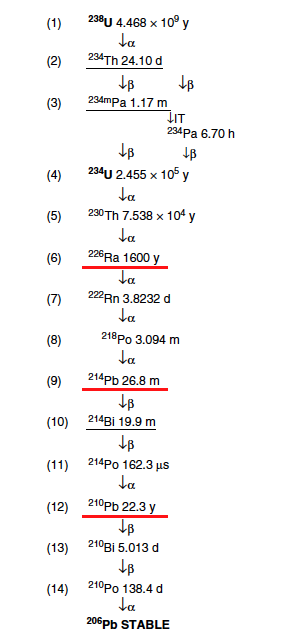
\includegraphics[height=0.8\textheight]{Imagenes/UDacay.png}
 \caption{Serie de desintegración de \UDosTresOcho\, (imagen modificada de \cite{gilmore2008}).}\label{Fig-SerieUranio}
\end{figure}	
\PbCero\, es el radionúclido de principal interés en este trabajo. Se trata de un isótopo radiactivo de Pb, de origen natural, emisor de radiación $\beta^{-}$ (y muy débilmente emisor $\alpha$, con una probabilidad de emisión de 0.0000019 \% \cite{DataDecayEvaluation}) que pertenece a la serie radiactiva de \UDosTresOcho\ (Figura \ref{Fig-SerieUranio}). El 99.25 \% del uranio natural es \UDosTresOcho, que forma parte de la naturaleza de las rocas.
\vspace{0.5cm}
\\
Por otra parte, la actividad $A$ de un radionúclido en una muestra se define como el número de desintegraciones nucleares por unidad de tiempo. La actividad se mide en Becquerelio (Bq) en el Sistema Internacional y es igual al número de desintegraciones nucleares por segundo. La actividad $A$ es proporcional al número de átomos radiactivos $N$ presentes en la muestra en el tiempo $t$ como
\begin{equation}\label{Eq-Desintegracion1}
A = - \dfrac{\text{d}N}{\text{d}t} = \lambda\,N,
\end{equation}
donde la constante de proporcionalidad $\lambda$, conocida como constante de desintegración, depende del núcleo radiactivo y tiene unidades recíprocas de tiempo. El semiperiodo $T_{\frac{1}{2}}$ de un radionúclido es el tiempo en el cual la actividad decrece a la mitad de su valor original. El semiperiodo se relaciona con la constante de desintegración $\lambda$ mediante la ecuación
\begin{equation}
T_{\frac{1}{2}} = \dfrac{\ln(2)}{\lambda}.
\end{equation}
Si $N_0$ y $A_0$ son respectivamente el número de núcleos radiactivos y la actividad en $t=0$, la Ecuación \ref{Eq-Desintegracion1} permite calcular la cantidad de átomos radiactivos $N$ y actividad $A$ en función del tiempo $t$,
\begin{equation}
N(t) = N_0\,\exp(-\lambda\,t), \hspace{2cm} A(t) = A_0\,\exp(-\lambda\,t).
\end{equation}
Para tiempos largos, en series radiactivas como la serie natural de \UDosTresOcho\, (Figura \ref{Fig-SerieUranio}), la actividad del núcleo descendiente $A_{\text{desc}}$ en relación a la actividad del núcleo progenitor $A_{\text{prog}}$ es \cite{gilmore2008}
\begin{equation}
A_{\text{desc}} = \dfrac{T_{\frac{1}{2}, \text{prog}} }{T_{\frac{1}{2}, \text{prog}}  - T_{\frac{1}{2}, \text{desc}}}\, A_{\text{prog}},
\end{equation}
donde $T_{\frac{1}{2}, \text{prog}}$ y $T_{\frac{1}{2}, \text{desc}}$ son los semiperíodos del núcleo progenitor y del núcleo descendiente, respectivamente. Cuando $T_{\frac{1}{2}, \text{prog}} \gg T_{\frac{1}{2}, \text{desc}}$, se produce la igualdad de las actividades, $A_{\text{desc}} = A_{\text{prog}}$, que se conoce como equilibrio secular.
\\
\\
En el caso de un sistema cerrado, los núcleos descendientes de la cadena de \UDosTresOcho\, deberían estar en equilibrio con el progenitor, pues su semiperíodo es muy inferior al de \UDosTresOcho, $T_{\frac{1}{2}}(^{238}\text{U}) = 4.468(5)\times 10^9 \text{ años}$  \cite{DataDecayEvaluation}. Algunos de los descendientes emisores de rayos gamma principales son el $^{234}$Th, $^{234\text{m}}$Pa, \Ra, $^{214}$Pb, $^{214}$Bi y \PbCero\, \cite{gilmore2008}. En sistemas cerrados, \PbCero\, y \Ra se encuentran en equilibrio debido a que estos y los radionúclidos intermedios (por ejemplo \PbCuatro) se encuentran confinados dentro de la matriz ambiental \cite{sanchez2012radiocronologia}.
\\
\\
\PbCero\, tiene un semiperíodo de $T_{\frac{1}{2}}(^{210}\text{Pb}) = 22.23(12)\text{ años}$ \cite{DataDecayEvaluation} y el esquema de desintegración se muestra en la Figura \ref{Fig-Squema210Pb}. El 80.2 \% de los núcleos de \PbCero\, decaen mediante desintegración $\beta^{-}$ al \Bi\, en estado excitado, el cual llega al estado fundamental mediante la emisión de un rayo gamma de 46.539(1) keV. La desintegración $\beta^{-}$ es un proceso de conversión donde un neutrón $n$ se convierte en un protón $p$	, un electrón o partícula $\beta^{-}$ y un antineutrino $\overline{\nu}$ \cite{gilmore2008}. La medida de la actividad de \PbCero\, a través del rayo gamma de 46.54 keV permite fechar núcleos sedimentarios hasta aproximadamente cinco veces el tiempo de vida media, es decir, permite fechar núcleos hasta $\sim$ 100 años de antig\"uedad, lo que incluye la época de mayor crecimiento de población y desarrollo industrial en el planeta, a partir de 1950. 
\begin{figure}[h]
\centering
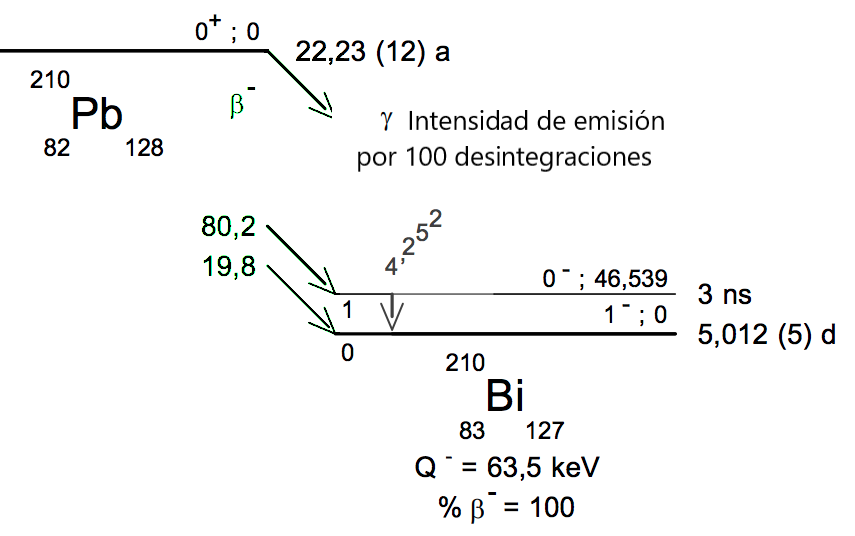
\includegraphics[width=0.5\textwidth]{Imagenes/210Pb-2.png}
\caption{Esquema de desintegración de \PbCero\, \cite{DataDecayEvaluation}.}\label{Fig-Squema210Pb}
\end{figure}
	\subsection{Núcleos sedimentarios}\label{SubSec-Sedimentos}
Para el estudio del Cambio Global se utilizan habitualmente núcleos sedimentarios porque:
\begin{itemize}
\item son concentradores de muchas de las substancias presentes en los sistemas acuáticos (por ejemplo, la mayor parte de los contaminantes),
\item son relativamente fáciles de colectar y analizar, y
\item son integradores de información en el tiempo.
\end{itemize}
Debido a la alta reactividad de Pb con las partículas, el depósito y desintegración de \PbCero\, permite establecer el marco temporal del núcleo sedimentario siempre que se cumpla el principio de superposición, y que los sedimentos no se hayan mezclado después de haber sido depositados.
\\
\\
El muestreo de núcleos sedimentarios se realiza habitualmente en tubos cilíndricos de longitud variable, típicamente del orden de 50 - 100 cm (Figura \ref{Fig-MuestreoNucleoSed}). Los sedimentos pueden ser extrudidos o expuestos longitudinalmente, para ser cortados en secciones de espesor variable (idealmente de 1 cm). La medida de \PbCero\, puede ser realizada directamente mediante espectrometría de rayos gamma (Sección \ref{Secc-IntroEspectrometriaGamma}) o mediante espectrometría de partículas alfa, a través del análisis de su nieto radiactivo \Po, bajo la suposición de equilibrio secular entre ambos radionúclidos (Figura \ref{Fig-SerieUranio}). La espectrometría de partículas alfa requiere un procesamiento radioquímico sencillo, poca cantidad de muestra y permite obtener un recuento rápido de la concentración para obtener una estadística fiable.
\begin{figure}[h]
\centering
  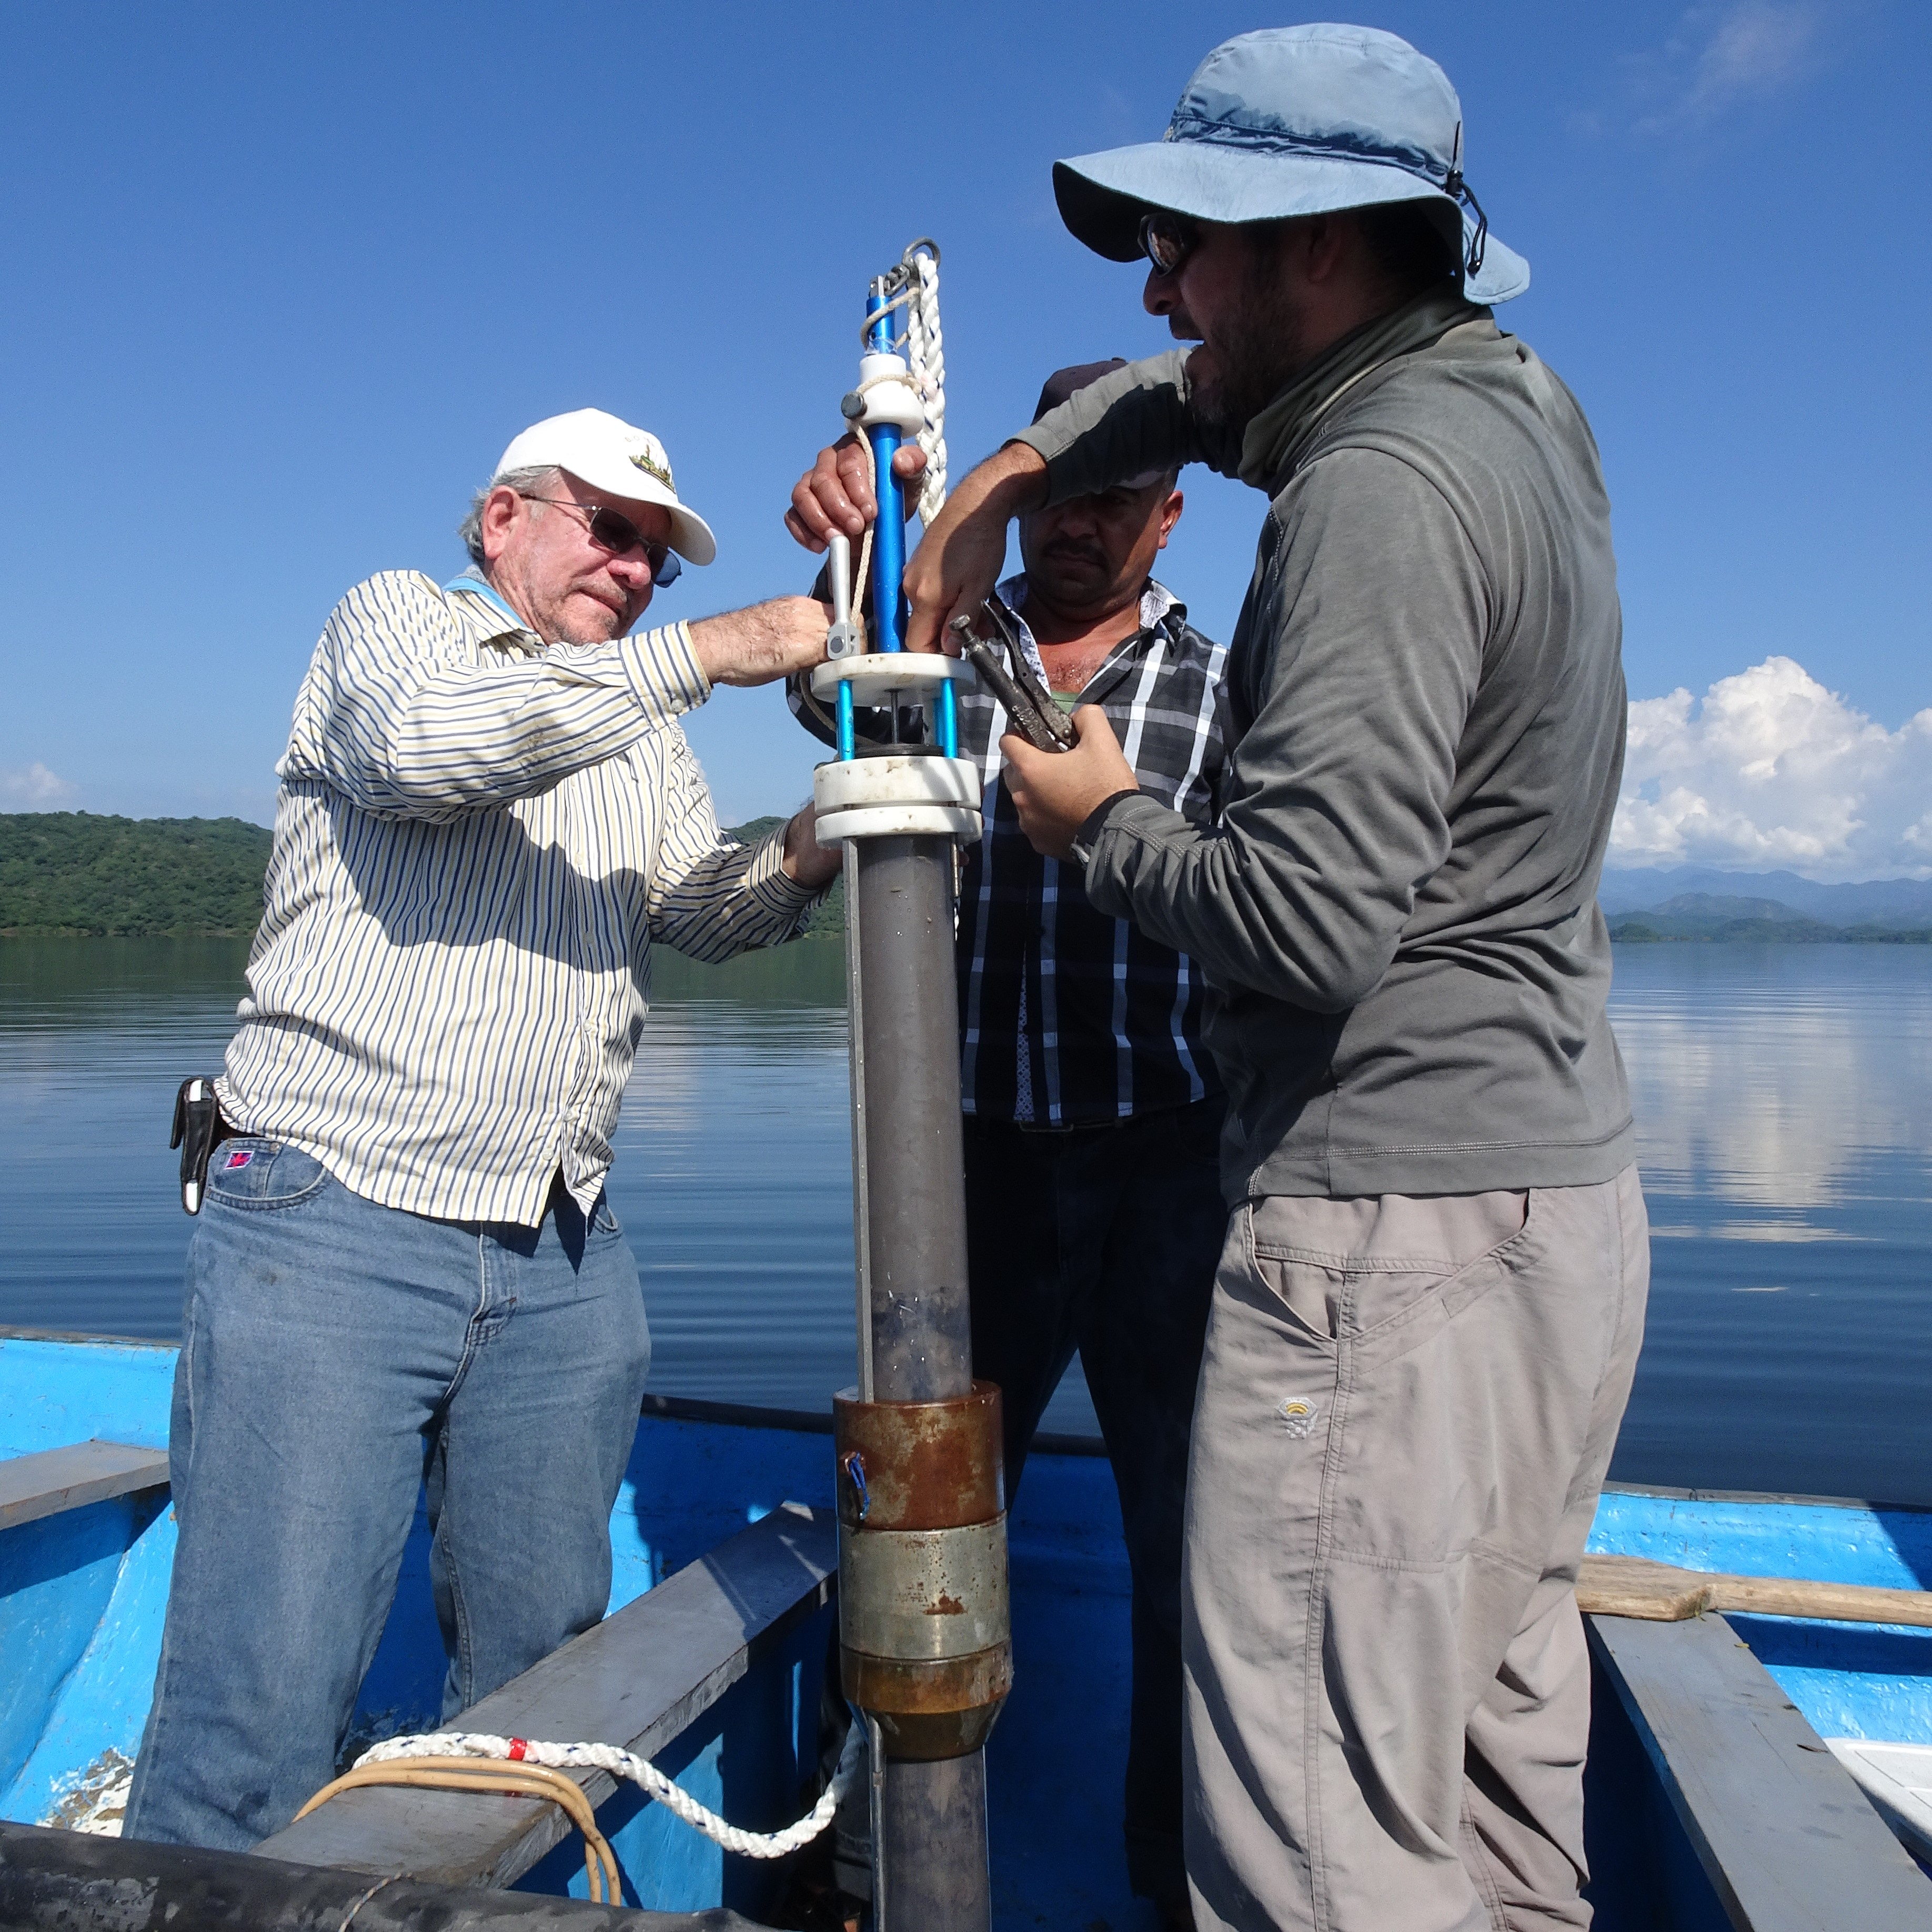
\includegraphics[height = 0.35\textheight]{Imagenes/DSC01875-CUADRADA.JPG}
  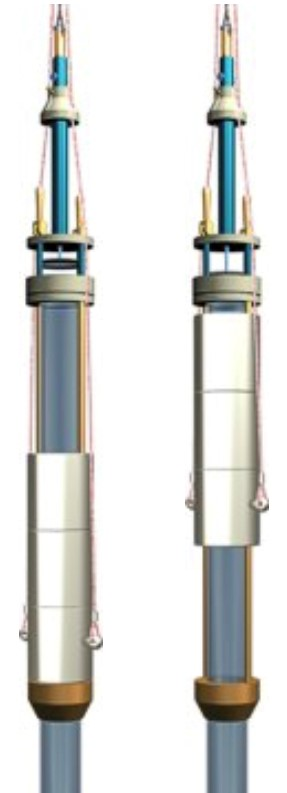
\includegraphics[height = 0.35\textheight]{Imagenes/IMG_2280.jpg}
\caption{Izquierda: muestreo de un núcleo sedimentario en un ambiente lacustre. Derecha: nucleador \cite{Uwitec}.}\label{Fig-MuestreoNucleoSed}
\end{figure}
	\subsection{El ciclo de \PbCero\, en ecosistemas acuáticos}\label{SubSec-Ciclo}
La actividad de \PbCero\, presente en los sedimentos puede tener diversos orígenes (Figura \ref{Fig-Ciclo210Pb}) \cite{KOIDE1972442}:
\begin{itemize}
\item La desintegración de \Rn, núcleo precursor de \PbCero, que es un gas noble y puede escapar de la tierra hacia la atmósfera después de la desintegración del núcleo progenitor \Ra. \Rn\, decae en la atmósfera en una corta serie de núcleos de vida media corta ($\sim$ minutos) hasta \PbCero. Debido a la alta reactividad del Pb con las partículas, el \PbCero\, se une a partículas en suspensión y sedimenta al fondo de los sistemas acuáticos.  
\item \Rn\, puede escapar de la litosfera directamente a los cuerpos de agua y decaer en \PbCero, que también sedimenta al fondo. La suma de este componente y la anterior se denomina \PbCero\, en exceso, \PbCeroEx, que es la base del fechado de sedimentos con \PbCero.
\item \Rn\, que no escapa sino que se desintegra \textit{in situ} y decae en \PbCero, conocido como $^{210}$Pb$_\text{base}$. Para sistemas cerrados por tiempos superiores a 150 años, $^{210}$Pb$_\text{base}$ se encuentra en equilibrio con el radionúclido \Ra\, \cite{SANCHEZCABEZA2012183}, con $T_{\frac{1}{2}}$ (\Ra) = 1600(7) años \cite{DataDecayEvaluation}. 
\end{itemize}
\begin{figure}[h]
 \centering
 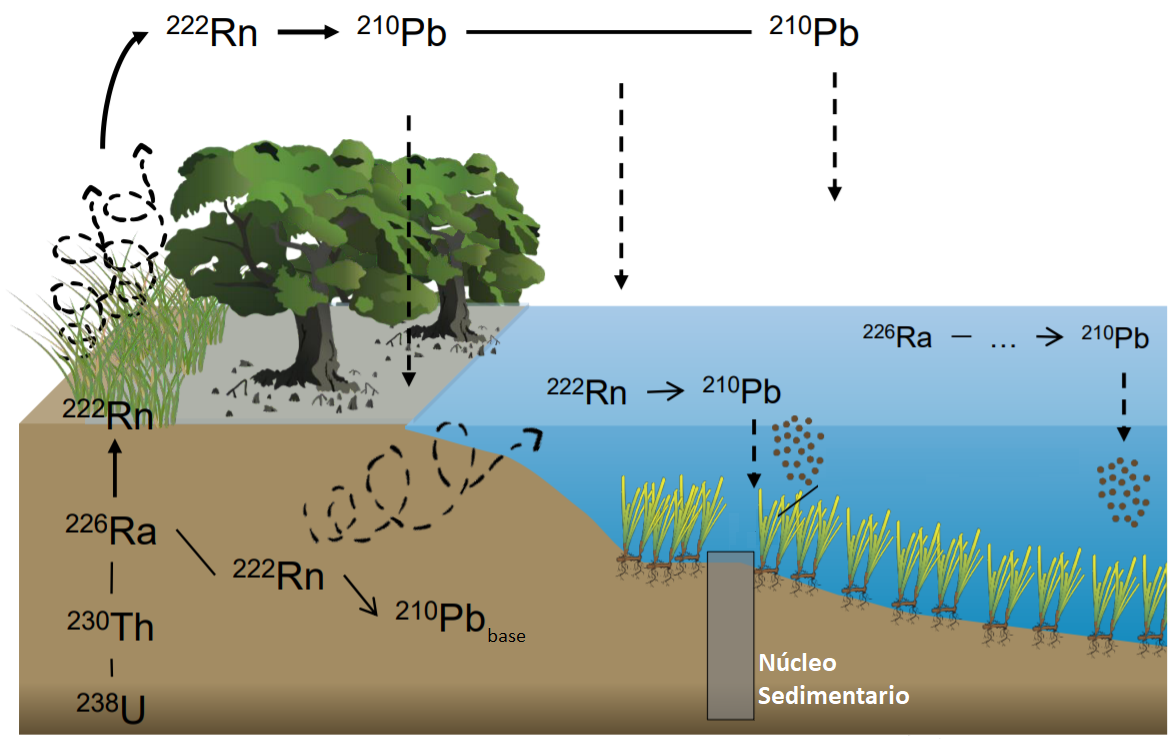
\includegraphics[width=\textwidth]{Imagenes/Ciclo210PbAcuatico.png}
 \caption{Ciclo de \PbCero\, en un sistema costero. Figura tomada de \cite{Foto210Pb}.}\label{Fig-Ciclo210Pb}
\end{figure}
La actividad total medida de \PbCero\, ($^{210}$Pb$_\text{total}$) es la suma de los procesos anteriores:
\begin{equation}\label{Eq-PbTotal}
^{210}\text{Pb}_\text{total} = ^{210}\text{Pb}_\text{base} + ^{210}\text{Pb}_\text{exc}.
\end{equation}
	\subsection{Fechado de núcleos sedimentarios}\label{SubSec-Fechado}
Los modelos de fechado de núcleos sedimentarios son utilizados para \cite{SANCHEZCABEZA2012183}
\begin{itemize}
\item Obtener la edad $t$ de cada sección del núcleo sedimentario en función de la profundidad $z$, es decir, construir un modelo de edad.
\item Calcular tasas de acumulación másica (MAR, en g cm$^{-2}$ año$^{-1}$) y sedimentarias (SAR, en cm año$^{-1}$) en función del tiempo.
\end{itemize}	
Un núcleo sedimentario se puede estudiar como la suma de secciones $i$, Figura \ref{Fig-EsquemaNucleoSed}. Cada sección $i$ presenta ciertas características definidas: masa, densidad, composición elemental, tiempo promedio de formación, actividad de \PbCero, entre otras, y a su vez, cada sección se encuentra en medio de las capas de corte. La nomenclatura de la sección $i$-ésima es un subíndice $_i$ y las capas se denotan mediante paréntesis $(i)$. 
\begin{figure}[h]
 \centering
 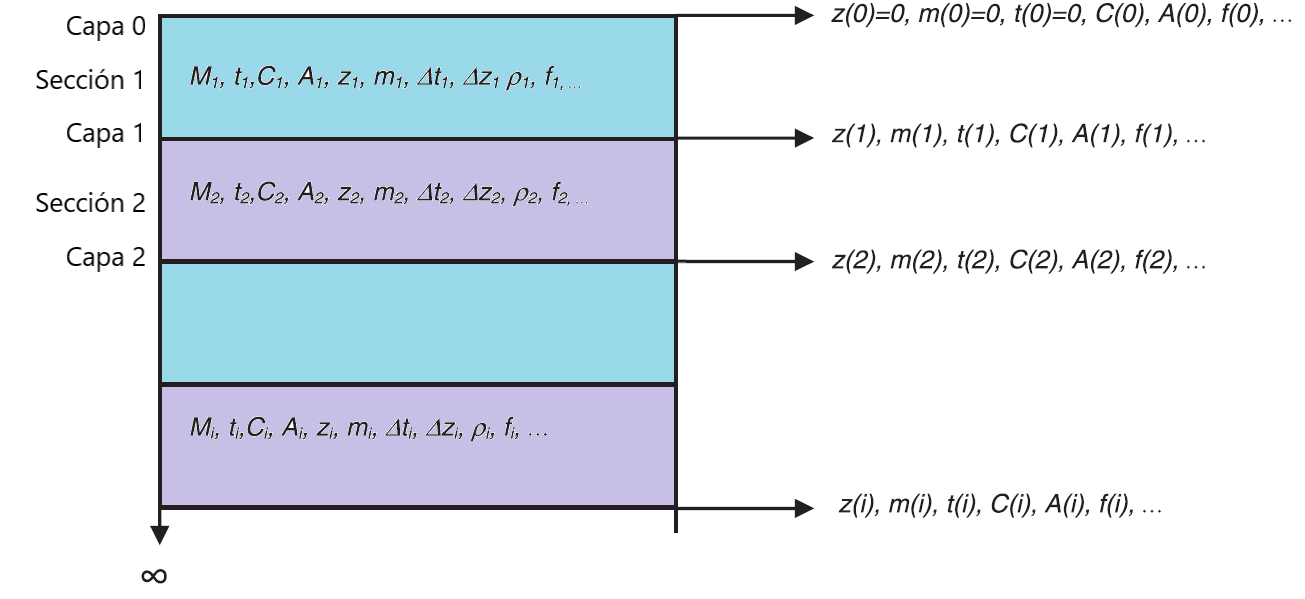
\includegraphics[width=\textwidth]{Imagenes/EsquemaNucleoSed-3.png}
 \caption{Parámetros relacionados con el fechado de un núcleo sedimentario. Imagen modificada de \cite{SANCHEZCABEZA2012183}.}\label{Fig-EsquemaNucleoSed}
\end{figure}	
\\ Algunos parámetros, constantes y definiciones relacionadas con el proceso de fechado son:
\begin{itemize}
\item $T_{\frac{1}{2}}$, $\lambda$: Tiempo de vida media y constante de desintegración del \PbCero, respectivamente. $T_{\frac{1}{2}} = (22.23 \pm 0.12)$ años, $\lambda = (0.03118 \pm 0.00017)$ años$^{-1}$.
\item $S$: Área transversal del núcleo sedimentario. Se calcula utilizando el diámetro interno del núcleo. 
\item $z(i)$: profundidad de la capa $i$-ésima. $z(i=0)=0$ m. 
\item $z_i$: profundidad promedio de la sección $i$-ésima, $z_i = \dfrac{z(i+1)+z(i)}{2}$. 
\item $\bigtriangleup z_i$: ancho de la sección, usualmente próximo a 1 cm. 
\item $\bigtriangleup m_i$: masa seca de la sección $i$-ésima determinada experimentalmente. 
\item $m(i)$: profundidad másica de la capa $i$-ésima. El proceso de fechado debe realizarse en función de la profundidad másica y no en función de la profundidad para tener en cuenta la compactación  del núcleo. $m(i) = \displaystyle \sum_{j=1}^{j=i} \dfrac{\bigtriangleup m_j}{S}$, $m(0) = 0$.
\item $m_i$: profundidad másica promedio de la sección $i$-ésima. 
\item $\rho_i = \dfrac{\bigtriangleup m_i}{S\, \bigtriangleup z_i}$: densidad promedio seca de la sección $i$. 
\item $t(i)$: tiempo transcurrido desde la formación de la capa $i$, $t(0)=0$ años.
\item $\bigtriangleup t_i = t(i) - t(i-1)$: periodo de formación de la sección $i$. 
\item $A_i$: Actividad específica de \PbCeroEx\, de la sección $i$-ésima. 
\item $A_i (t=0)$: Actividad específica de \PbCeroEx\, de la sección $i$-ésima cuando se formó. 
\item $A(i)$: Actividad específica de \PbCeroEx\, de la capa $i$-ésima. 
\item $\bigtriangleup \mathbb{A}_i$: depósito de \PbCeroEx\, en la sección $i$, actividad por unidad de área. $\bigtriangleup \mathbb{A}_i = \dfrac{A_i\,\bigtriangleup m_i}{S}$
\item $s(i)$, $s_i$: tasa de acumulación sedimentaria de la capa $i$ y promedio de la sección $i$, respectivamente. 
\item $r(i)$, $r_i$: tasa de acumulación másica de la capa $i$ y promedio de la sección $i$, respectivamente. 
\item $f(t)$, $f_i$, $f(i)$: flujo a la superficie del sedimento, flujo promedio hacia la superficie del sedimento durante la formación de la sección $i$ y flujo hacia la capa $i$ cuando fue formada, respectivamente. 
\end{itemize}
Cuando la capa $i$-ésima es formada ($t=0$), la concentración de la capa $A(i, t=0)$ es
\begin{equation}\label{Eq-Ci}
A(i, t=0) = \dfrac{f(i)}{r(i)}.
\end{equation}
El modelo de Flujo Constante (CF, por sus siglas en inglés) asume que el flujo de \PbCeroEx\, hacia la superficie del sedimento es constante. $f_i = f(i) = f$. La Ecuación \ref{Eq-Ci} en el modelo de Flujo Constante se puede rescribir como 
\begin{equation}\label{Eq-FC}
f = A(i,t=0)\, r(i).
\end{equation}
La anterior ecuación implica que las concentraciones iniciales $C(i, t=0)$ y la tasa de acumulación másica $r(i)$ de diferentes capas pueden ser diferentes pero deben ser inversamente proporcionales. 
\\ \\ 
El depósito acumulado hasta la capa $i$-ésima $\mathbb{A}(i)$ es 
\begin{equation}
\mathbb{A}(i) = \sum_{j=i+1}^{j\rightarrow \infty} \bigtriangleup \mathbb{A}_j = \int_m^\infty A\, dm =  
\int_m^\infty \dfrac{f}{r}\,\exp(-\lambda\,t)\, dm =  \dfrac{f}{\lambda}\,\exp(-\lambda\,t).
\end{equation}
Para $t=0$, $z=0$ y $m=0$, entonces 
\begin{equation}
f = \lambda\,\mathbb{A}(t=0),
\end{equation}
donde $\mathbb{A}(t=0)$ es el flujo de \PbCeroEx\, en la superficie del sedimento. Entonces el depósito acumulado por debajo de la la capa $i$-ésima es 
\begin{equation}
\mathbb{A}(i) = \mathbb{A}(0)\,\exp(-\lambda\,t).
\end{equation}
De la anterior ecuación se puede calcular la edad de la capa, a saber, 
\begin{equation}\label{Eq-Fechado}
t(i) = \dfrac{1}{\lambda}\,\ln\left(\dfrac{\mathbb{A}(0)}{\mathbb{A}(i)}\right) = \dfrac{1}{\lambda}\,\ln\left(\dfrac{\sum_{j=1}^\infty A_j\, m_j}{ \sum_{j=i+1}^\infty A_j\, m_j}\right).
\end{equation}
\section{Espectrometría de rayos gamma}\label{Secc-IntroEspectrometriaGamma}
La espectrometría de rayos gamma es una técnica no destructiva que permite cuantificar de forma directa \PbCero\,y otros radionúclidos de interés. Los detectores de rayos gamma son más costosos que los detectores de espectrometría de partículas alfa, la calibración es compleja y, dada la baja actividad de \PbCero\, en muestras ambientales ($\sim$ 20 Bq kg$^{-1}$), se requiere largos tiempos de medida para obtener una estadística aceptable. Las muestras deben estar secas, molidas, homogeneizadas, y el detector debe ser calibrado con patrones similares a las muestras en geometría y densidad, cosa que no es siempre posible.
\\ \\ 
En radiocronología de núcleos sedimentarios se utilizan detectores de germanio hiper-puro en configuración de pozo y la calibración se realiza usando patrones certificados.
	\subsection{Interacción de la radiación gamma con la materia}\label{SubSec-Interaccion}
\PbCero\, es cuantificado mediante espectrometría de rayos gamma a través de la interacción de fotones de 46.54 keV con el material detector. Los canales de interacción entre los rayos gamma y la materia dependen de la energía de la radiación incidente. Los rayos gamma en el intervalo energético 40 keV - 2 MeV  interactúan con la materia a través de los siguientes procesos:
\begin{equation*}
    \begin{array}{L@{\quad}c@{{}\rightarrow{}}c}
       Efecto fotoeléctrico:	& \gamma+\text{átomo} & \text{átomo}^{+} + e^{-} \\
       Efecto Compton:      & \gamma+ e^{-} & \gamma^{'} + e^{- '} \\
       Formación de pares: 	& \gamma+\text{núcleo} & e^{-}e^{+}+\text{núcleo}
    \end{array}
\end{equation*}
		\subsubsection{Efecto fotoeléctrico}
El efecto fotoeléctrico ocurre debido a la interacción entre el rayo gamma y uno de los electrones atómicos. Esta interacción genera la emisión del electrón de su capa atómica y deja al átomo en estado excitado. La energía cinética $E_c$ del electrón eyectado es \cite{gilmore2008}
\begin{equation}
E_c = E - E_b,
\end{equation}
donde $E$ y $E_b$ denotan la energía del rayo gamma y la energía de ligadura del electrón, respectivamente. El átomo se desexcita mediante la emisión de un rayo X característico de la transición de un electrón de capas más a menos energéticas. La capa atómica desde la cual el electrón es emitido depende de la energía de la radiación gamma $E$. 
\\ \\
La sección eficaz de la absorción fotoeléctrica $\sigma_{\text{foto}}$ presenta un valor máximo para energías de radiación gamma incidente cercanas a la energía de ligadura de los electrones de la capa atómica K. En un intervalo  $13.6$ eV $<E<m_e\,c^2 $ = 1.022 MeV, $\sigma_{\text{foto}}$ presenta una dependencia fuerte con la energía, y para energías superiores a $m_e\,c^2$ la dependencia de la sección eficaz fotoeléctrica es suave respecto a la energía, \cite{grupen2008particle}
\begin{equation}
\sigma_{\text{foto}} \propto  
  \begin{cases}
    Z^5\, E^{-3.5},	& 13.6 \text{ eV} < E<m_e\,c^2, \\
    Z^5\, E^{-1},	& E > m_e\,c^2.
  \end{cases}
\end{equation}
		\subsubsection{Efecto Compton}
La interacción Compton consiste en una colisión elástica entre un fotón y un electrón. El rayo gamma con energía $E$ interacciona directamente con el electrón y le transfiere parte de su energía. La energía del electrón después de la colisión es \cite{gilmore2008}
\begin{equation}\label{Eq-Energia-Gamma-Nueva}
E_e = E - E' = E - E \left( 1+\dfrac{E}{m_e\,c^2}\,(1-\cos(\theta)) \right)^{-1},
\end{equation}
donde $\theta$ denota el ángulo para el rayo gamma después de la interacción  (Figura \ref{Fig-Compton}), $E$ y $E'$ son la energía del rayo gamma antes y después de la colisión, respectivamente. El comportamiento de la sección eficaz de Compton, $\sigma_\text{Comp}$, presenta las siguientes relaciones: \cite{grupen2008particle}
\begin{equation}
\sigma_\text{Comp} \propto
  \begin{cases}
    \sigma_{\text{Thompson}}(1-2\,\epsilon),	& E \ll m_e\,c^2, \\
    \log(\epsilon)\, \epsilon^{-1} \,Z,		&  E \gg m_e\,c^2,
  \end{cases}
\end{equation}
donde $\epsilon = \dfrac{E}{m_e\,c^2}$ y $\sigma_{\text{Thompson}}$ = 0.66 barn, 1 barn = $10^{-28}$ m$^{2}$.
		\begin{figure}[h]
		\centering
		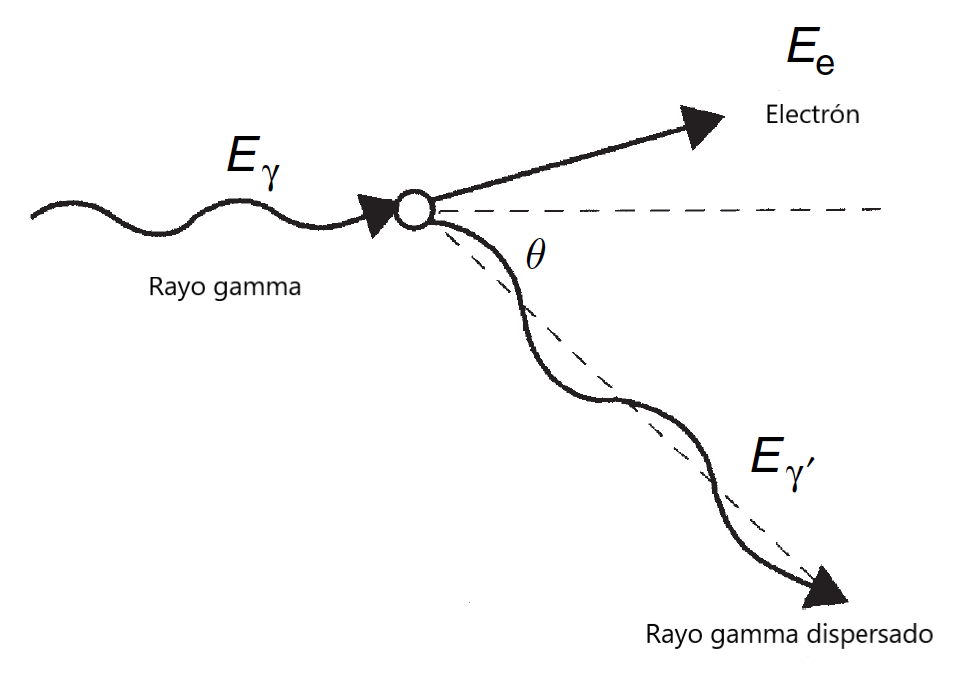
\includegraphics[width=0.48\textwidth]{Imagenes/Compton-2.png}
		\caption{Representación esquemática del efecto Compton, \cite{gilmore2008}.}\label{Fig-Compton}
		\end{figure}
		\subsubsection{Formación de pares}
A diferencia del efecto fotoeléctrico y Compton, la producción de pares es el resultado de la interacción del rayo gamma con el átomo en su conjunto. El proceso ocurre dentro del campo de Coulomb del núcleo y produce la conversión de un rayo gamma en un par electrón - positrón. Para que este proceso sea energéticamente posible, la energía del rayo gamma debe ser superior a la suma de la energía en reposo del electrón y positrón $E > 1.022$ MeV.
\vspace{0.5cm} \\
El positrón creado encuentra otro electrón y se aniquila emitiendo dos rayos gamma diametralmente opuestos de 511 keV cada uno. Para $E \gg m_e\,c^2$, la sección eficaz de la producción de pares $\sigma_{\text{pares}}$ se puede escribir como \cite{grupen2008particle}
\begin{equation}
\sigma_{\text{pares}} = \dfrac{7}{9}\,\dfrac{N_A}{A}\,\dfrac{1}{X_0}, \hspace{1cm}\text{con}\hspace{1cm} X_0 \propto\left[Z^2\,\log\left(\dfrac{183}{Z^{1/3}}\right) \right]^{-1}, 
\end{equation}
donde $N_A$ es el número de Avogadro y $A$ el número de nucleones.
\\ \\ 
La Figura \ref{Fig-Secciones} muestra la sección eficaz total por átomo en función de la energía para fotones sobre germanio ($Z=32$) y las contribuciones parciales de cada proceso de acuerdo al intervalo energético \cite{NistGE}. Para una energía de 46.54 keV (\PbCero) el proceso dominante es el efecto fotoeléctrico, sin embargo, para una energía de 351.93 (\PbCuatro) el efecto Compton es el proceso dominante. 
\begin{figure}[h]
\centering
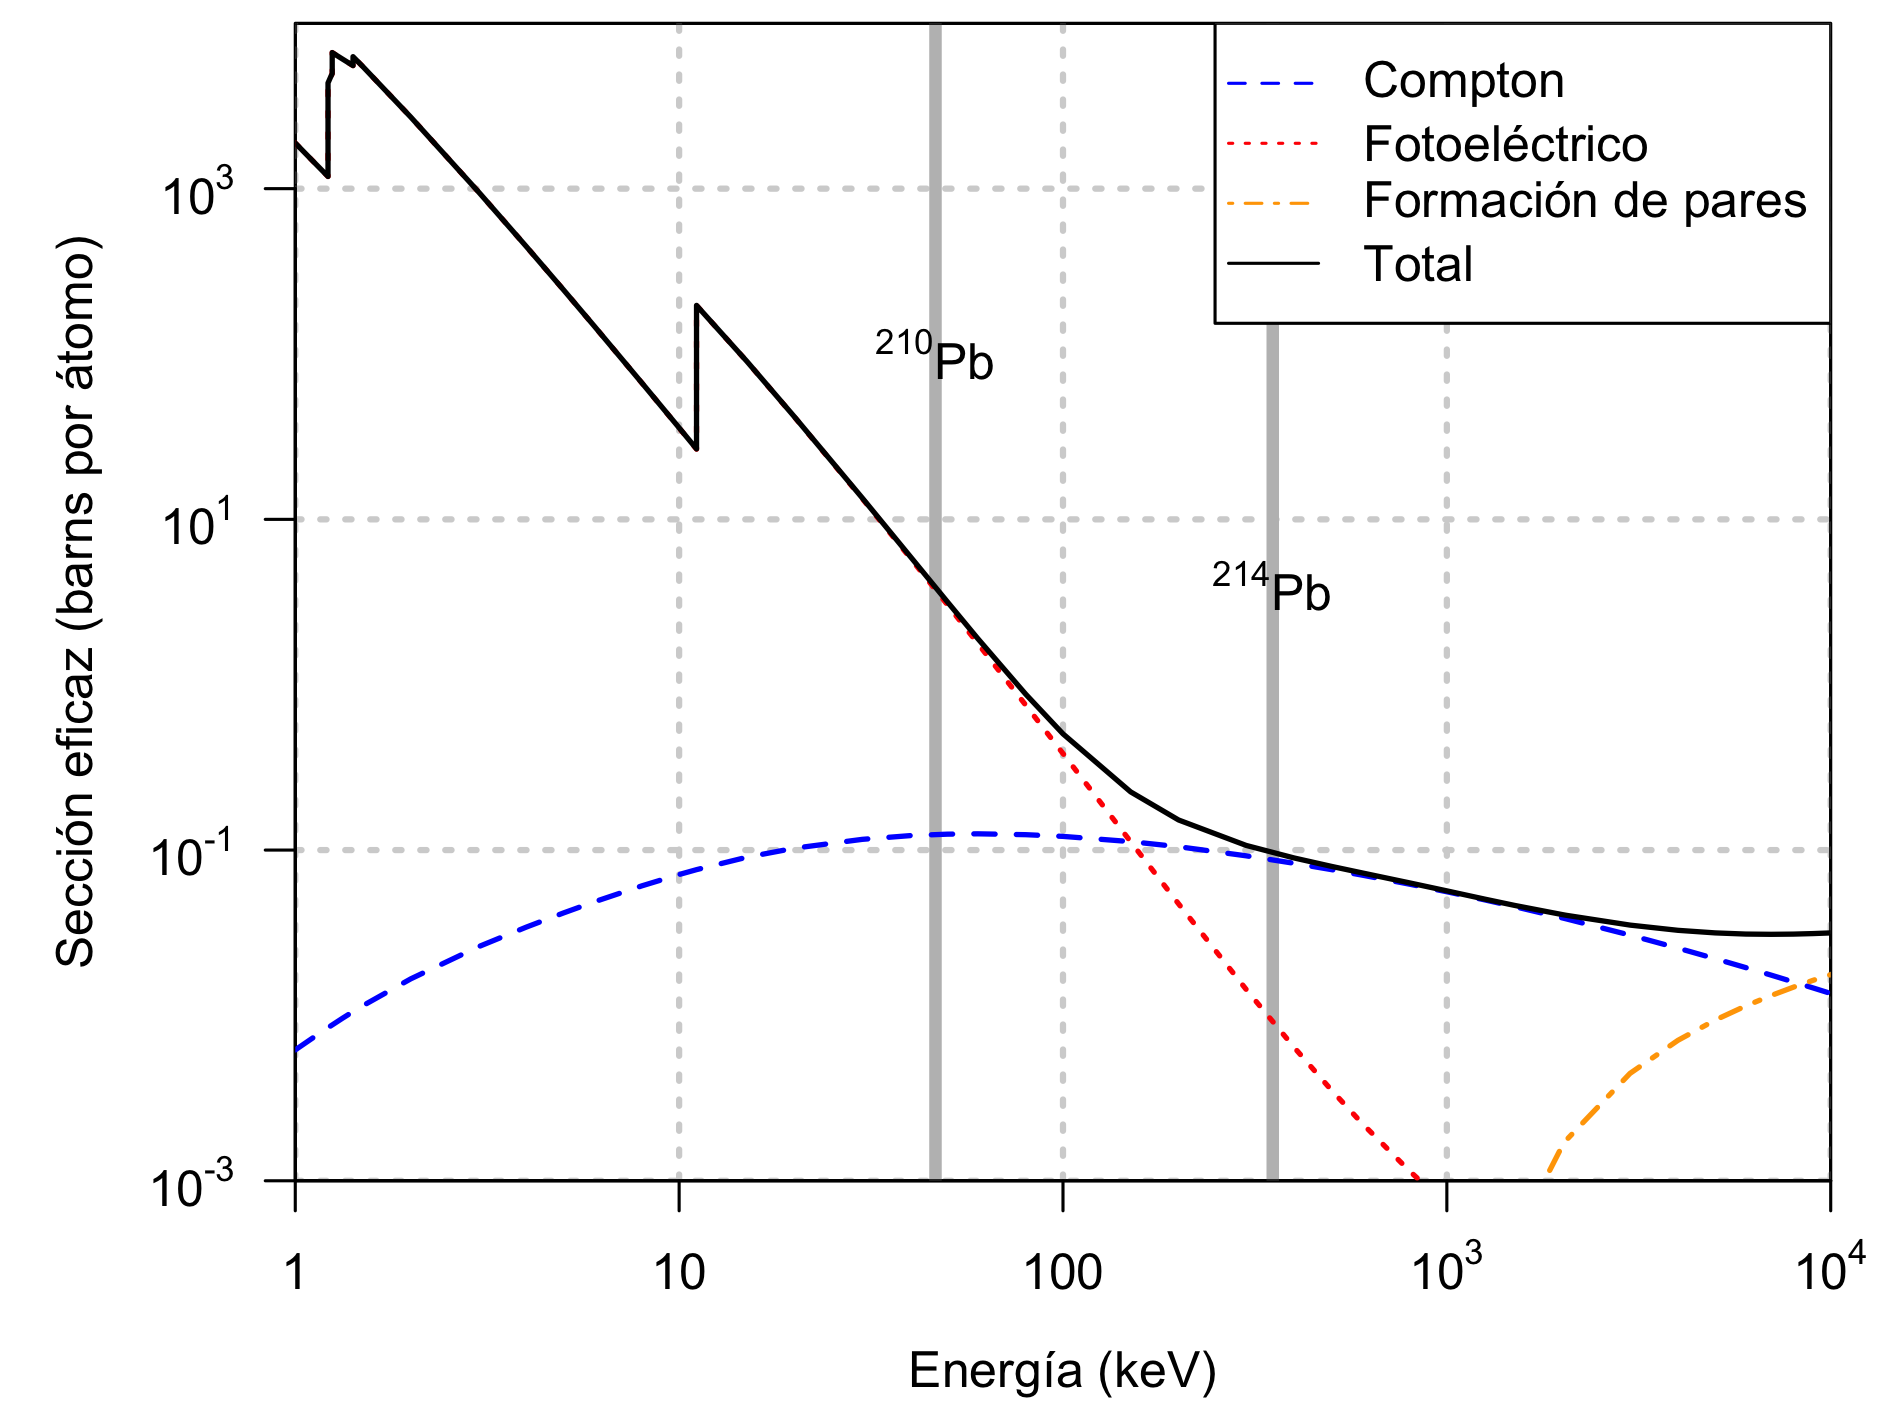
\includegraphics[width=0.7\textwidth]{Imagenes/CrossSectionGe.png}
\caption{Sección eficaz total de fotones sobre germanio $(Z=32)$. Se observan las contribuciones parciales de los procesos: fotoeléctrico, Compton y formación de pares.}\label{Fig-Secciones}
\end{figure}
		\subsubsection{Coeficiente másico de atenuación}
La interacción de la radiación con la materia se cuantifica de forma global a través del coeficiente másico de atenuación  $\dfrac{\mu}{\rho}$. Cuando un haz monoenergético y colimado de radiación gamma con intensidad inicial $I_0$ incide sobre un material de densidad $\rho$, su intensidad $I$ decrece siguiendo la ley de atenuación exponencial \cite{CUTSHALL1983309, NIST}
\begin{equation}\label{Eq-Atenuacion}
\dfrac{I}{I_0} = \exp\left[-\dfrac{\mu}{\rho}\,\rho\,x\right].
\end{equation}
La anterior ecuación es una aproximación porque asume que los rayos gamma perfectamente colimados atraviesan la muestra sin desviarse, si bien los fotones pueden emerger en ángulos diversos \cite{IURIAN2018151}. Los valores de $\dfrac{\mu}{\rho}$ para muchos materiales se encuentran ya reportados en \cite{NIST}.
\\
\\
La sección eficaz total $\sigma_\text{total}$, que es la suma de las secciones eficaces de los procesos considerados para determinada energía $E$, $\sigma_\text{total} = \sigma_\text{foto} + \sigma_\text{Comp} + \sigma_\text{pares} + ...$, se relaciona con el coeficiente másico de atenuación mediante \cite{NIST}
\begin{equation}\label{Eq-Mu}
\dfrac{\mu}{\rho} = \dfrac{\sigma_\text{total}}{u\,A},
\end{equation}
donde $\rho$ es la densidad del material, $u$ es la unidad de masa atómica y $A$ el número de nucleones. Por lo tanto, $\dfrac{\mu}{\rho}$ es un parámetro que depende de la energía del rayo gamma incidente y del material.
	\subsection{Detectores de Ge hiper-puro}\label{SubSec-DetecGe}
Los detectores de Ge hiper-puro son semiconductores, que presentan un comportamiento intermedio entre los materiales conductores y los materiales aislantes. La diferencia de energía entre la banda de valencia y la banda de conducción (gap - banda prohibida de energía) es de 0.67 eV, lo que implica que los electrones pueden ser excitados térmica u ópticamente. 
\\ \\
Los detectores semiconductores (como Si, Ge y GeAs) pueden ser entendidos  como cámaras de ionización de estado sólido. Debido a su alta densidad en comparación con los gases, los volúmenes de los detectores pueden ser muy inferiores. Estos se polarizan con dos electrodos que generan un campo eléctrico encargado de recoger los pares electrón-hueco producidos en el material. Debido a que el gap es pequeño, la cantidad de pares electrón-hueco producidos por unidad de energía depositada es alta, por lo que su resolución energética es muy buena. Sus principales aplicaciones son la espectrometría de rayos gamma y de partículas cargadas con alta resolución energética.
\\ \\
Los detectores pueden ser intrínsecos o dopados. Los detectores dopados pueden ser de tipo n, tipo p, compensados o altamente dopados. El tipo de detector en los detectores dopados depende de la valencia del material agregado. La unión de un semiconductor tipo n y tipo p crea una región de agotamiento, o \textit{depletion region}, importante para la detección de la radiación. El campo eléctrico que se crea en la región de desequilibrio causa que cualquier electrón o hueco creado en esta zona tienda hacia la zona de tipo n o de tipo p, respectivamente \cite{knoll2010radiation}. 
\\\\
Los detectores semiconductores intrínsecos, no dopados, son materiales de alta pureza (Tabla \ref{Table-PropiedadesSiGEe}). Algunas características de los detectores semiconductores son:
\begin{itemize}
\item Densidad elevada en comparación con detectores gaseosos. Esto implica una mayor pérdida de energía en distancias cortas y efectos difusivos más cortos, generando resoluciones espaciales de hasta 10 $\mu$m.
\item Baja energía de ionización (pocos eV para crear un par electrón – hueco) en comparación con detectores gaseosos (20 - 40 eV para crear un par de iones) o centelladores (400 - 1000 eV para crear un fotón).
\item Los detectores de Ge son ampliamente utilizados en física nuclear y necesitan refrigeración debido a su banda de energía prohibida tan pequeña. Los detectores de Si pueden operar a temperatura ambiente y son materiales estándar para detectores de vórtices y trayectorias de partículas elementales en física de altas energías.
\item Su precio es elevado debido al volumen y pureza del material, electrónica asociada y sistema de refrigeración.
\end{itemize}
\begin{table}[h]
 \centering
 \caption{Propiedades de los detectores semiconductores intrínsecos Si y Ge \cite{bertolini1968semiconductor}.}\label{Table-PropiedadesSiGEe}
 \begin{tabular}{|c|c|c|c|}\hline
\rowcolor{Blue2} Propiedad & unidad & Si & Ge \\ \hline
\rowcolor{Blue1} Número atómico & & 14 & 32 \\
\rowcolor{Blue1} Peso atómico & u & 28.09 & 72.60 \\
\rowcolor{Blue1} Densidad a 300 K & g cm$^{-3}$ & 2.33 & 5.32 \\
\rowcolor{Blue1} Banda prohibida a 300 K & eV & 1.115 & 0.665 \\
\rowcolor{Blue1} Energía por cada par electrón - hueco & eV & 3.76 & 2.96 \\ \hline
 \end{tabular}
\end{table}
			\subsubsection{Detectores de Ge en configuración tipo pozo}\label{Sec-GePozo}
Los detectores de Ge en configuración tipo pozo (Figura \ref{Fig-WellDetectorORTEC}) son detectores coaxiales con un contacto negativo en una apertura circular que permite introducir muestras pequeñas en ella. Este tipo de detector proporciona un ángulo sólido próximo a $4\pi$ y, en un intervalo de energías entre 50 keV a 200 keV, una eficiencia absoluta cercana al 90 \%, mientras que la eficiencia absoluta de los detectores de Ge cilíndricos comunes es muy inferior al 50 \% \cite{gilmore2008}.
\vspace{0.5cm}\\
La eficiencia absoluta es función de la energía y depende de la configuración geométrica: dimensiones del detector, del pozo y naturaleza del material protector del mismo (usualmente una capa de Al). La eficiencia adquiere su valor máximo en la parte inferior del pozo. La  capacitancia  de un detector de Ge en configuración tipo  pozo  es  mayor que la de un detector equivalente coaxial de Ge, causando una peor resolución  \cite{gilmore2008}.
\begin{figure}[h]
\centering
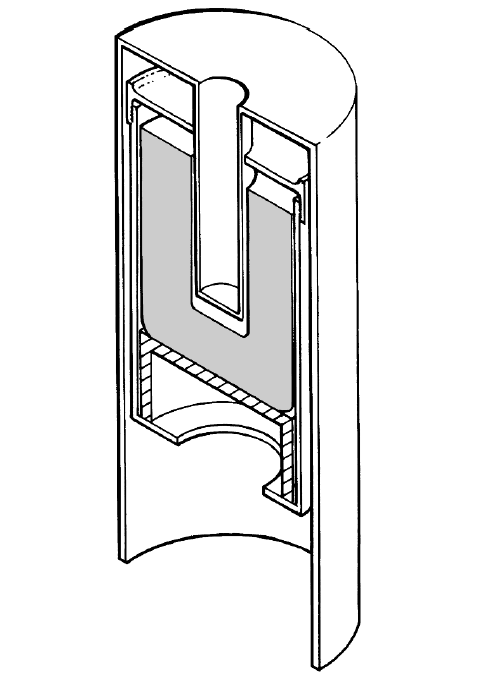
\includegraphics[width=0.25\textwidth]{Imagenes/WellDetectorSimply.png}
\caption{Vista isométrica simplificada de un detector de Ge en configuración de pozo \cite{WellDetectorORTEC}.}\label{Fig-WellDetectorORTEC}
\end{figure}
	\subsection{Eficiencia}\label{SubSec-Eficiencia}
La eficiencia absoluta $\epsilon$ para un sistema detector - fuente es la fracción entre el número de eventos emitidos y el número de eventos registrados, 
\begin{equation}
\epsilon = \dfrac{\text{Números de eventos registrados}}{\text{Número de eventos emitidos por la fuente}}.
\end{equation}
La eficiencia absoluta depende de i) la energía de la radiación emitida $E$, ii) la configuración geométrica detector – fuente, iii) la probabilidad de interacción de la radiación con el material –detector (eficiencia intrínseca), y iv)  la autoabsorción de la radiación en la muestra, entre otros factores. La eficiencia absoluta se puede escribir como \cite{PALACIOS200877}:
\begin{equation}
\epsilon(E) = \epsilon_{\text{intríseca}}(E)\cdot \epsilon(\Omega)\cdot\text{TCSC}\cdot \eta(E), 
\end{equation}
en donde 
\begin{itemize}
\item $\epsilon_{\text{intríseca}}(E)$ es la eficiencia intrínseca del detector a una energía determinada $E$. Se trata del número de eventos detectados en comparación con el número de eventos que impactan al detector. Es un parámetro básico y es independiente de la geometría fuente – detector,
\item $\epsilon(\Omega)$ es el factor geométrico. Esto se relaciona con la idea de un ángulo sólido entre la fuente y el detector,
\item TCSC (True Coincidence Summing Correction) es la corrección necesaria para corregir la detección simultánea de más de un rayo gamma o X. Este fenómeno es común en el caso de radionúclidos emisores gamma en cascada durante la desexcitación nuclear \cite{gilmore2008},
\item $\eta(E)$ es el factor de autoabsorción.
\end{itemize}
La actividad total $A$ (número de desintegraciones por unidad de tiempo) de un radionúclido en una muestra se determina mediante la ecuación: \cite{MONTALVANOLIVARES201734}
\begin{equation}\label{Eq-Actividad}
A = \dfrac{N(E) - B(E)}{\epsilon(E)\,f(E)\,t},
\end{equation}
en donde $N(E)$ es el número de cuentas netas para el fotopico $E$, $B(E)$ en el número de cuentas netas del fondo del detector para el mismo fotopico,  $\epsilon(E)$ es la eficiencia absoluta del sistema para la energía $E$, $f(E)$ es la probabilidad de emisión y $t$ es el tiempo de medición efectivo \cite{BELGIN201536}. La eficiencia absoluta puede ser determinada mediante calibración utilizando un patrón de geometría, composición y densidad similar a la muestra medida. Sin embargo, esto requiere la calibración directa de múltiples geometrías, densidades y composiciones en cada laboratorio, lo que es muy costoso y prácticamente imposible en la práctica.
\\ \\
Si bien una opción teóricamente posible es el cálculo de la eficiencia a través de simulación Monte Carlo de todos los procesos que ocurren desde la emisión del rayo gamma hasta su detección, una alternativa es la corrección de la eficiencia a través de funciones de transferencia \cite{VIDMAR2005603, MORERAGOMEZ201559}.
		\subsubsection{Factor de autoabsorción}\label{SubSecc-CoeffAtten}
La autoabsorción ocurre cuando parte de la radiación gamma emitida en una muestra extensa pierde parcial o totalmente su energía en la muestra misma y se cuantifica con el factor de autoabsorción $\eta(E)$. Este efecto es particularmente importante para rayos gamma de baja energía (como en el caso del \PbCero) y por lo tanto, afecta seriamente la exactitud de la medida de la actividad \cite{PILLEYRE2006323}.
\\
\\
El factor de autoabsorción depende de la composición, densidad y geometría de la muestra \cite{CUTSHALL1983309} y sigue la misma forma funcional que la Ecuación \ref{Eq-Atenuacion}. Para energías superiores a 80 keV, las diferencias en las composiciones químicas y densidades de muestras ambientales no afectan significativamente a $\dfrac{\mu}{\rho}$, pero sí afectan significativamente para energías inferiores \cite{VARGAS2002893}.
\\
\\
El factor de autoabsorción para materiales con diferentes composiciones puede calcularse mediante simulación Monte Carlo a través de la ecuación \cite{BELGIN201536, CUTSHALL1983309, APPLEBY1992228, APPLEBY2004423, PILLEYRE2006323, SAIDOU2007515}
\begin{equation}
\eta(E) = \exp\left(-\sum_i  \left( \dfrac{\mu}{\rho}\right)_i\,\rho_i\,x_i\right),
\end{equation}
donde el índice $i$ indica a los elementos que constituyen la muestra, $\left(\dfrac{\mu}{\rho}\right)_i$, $\rho_i $ y $x_i$ son el coeficiente másico de atenuación, densidad y concentración absoluta de cada elemento. 
		\subsubsection{ANGLE}\label{SubSec-ANGLE}
ANGLE es un software comercial que permite el cálculo de eficiencias mediante funciones de transferencia. La función de transferencia se define como el cociente de dos eficiencias y, por lo tanto, permite obtener la eficiencia $\epsilon$ partiendo de una eficiencia de referencia $\epsilon_\text{referencia}$. Una de las ventajas de esta estrategia es que las correcciones introducidas por la función de transferencia deberían ser pequeñas y, por lo tanto, sujetas a errores pequeños. 
\\
\\
La eficiencia se determina mediante ANGLE a través de un método semi-empírico que involucra i) la calibración experimental del detector para el cálculo de la eficiencia de referencia y, ii) una simulación mediante Monte Carlo que genera un \textit{ángulo sólido efectivo} de acuerdo a cierta composición y geometría. El ángulo sólido efectivo $\overline{\Omega}$ (Figura \ref{Fig-EffSolidAngle}) se define como \cite{JOVANOVIC2010385}
\begin{equation}\label{Eq-EffSolidAngle}
\overline{\Omega} = \int_{V_S, S_D}\, d\overline{\Omega} = \int_{V_S, S_D}\,\displaystyle F_{\text{aten.}}\,F_{\text{ef.}} \dfrac{\overrightarrow{TP}\cdot\hat{n}}{|\overrightarrow{TP}|^3}\,d\sigma,
\end{equation}
donde
\begin{itemize}
\item $V_S$: volumen de la muestra.
\item $S_D$: área del detector expuesta a la muestra.
\item $T$ y $P$ son puntos que varían sobre el volumen de la muestra y la superficie del detector, respectivamente. $\overrightarrow{TP}$ es la distancia entre estos dos puntos.
\item $d\sigma$: Elemento infinitesimal de área en $S_D$.
\item $\hat{n}$: vector unitario normal al diferencial de área $d\sigma$.
\item $F_{\text{aten.}}$: factor que toma en cuenta la atenuación del rayo gamma en dirección $\overrightarrow{TP}$.
\item $F_{\text{ef.}}$: probabilidad de interacción entre fotón y detector. 
\end{itemize}
La eficiencia $\epsilon$ para la energía de fotopico se calcula mediante la función de transferencia
\begin{equation}\label{Eq-Epsilon}
\epsilon = \dfrac{\overline{\Omega}}{\overline{\Omega}_\text{referencia}}\,\epsilon_\text{referencia}.
\end{equation}
La anterior ecuación asume que la eficiencia es una función intrínseca del detector y depende únicamente de la energía del rayo gamma.
\begin{figure}[h]
\centering
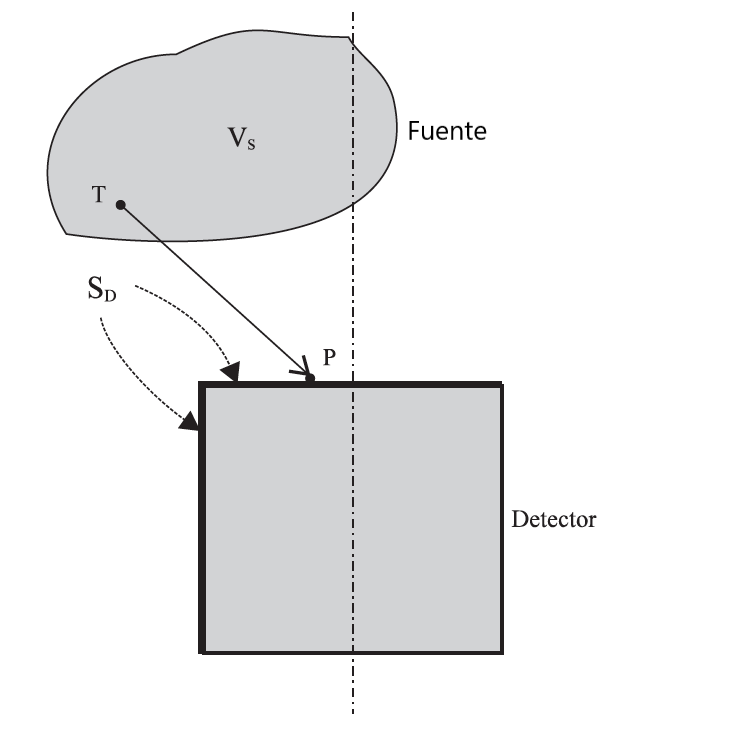
\includegraphics[width=0.45\textwidth]{Imagenes/EffectiveSolidAngle-2.png}
\caption{Variables involucradas en el cálculo del ángulo sólido efectivo, Ec. (\ref{Eq-EffSolidAngle}), para encontrar eficiencias a través del software ANGLE mediante la Ecuación \ref{Eq-Epsilon}.}\label{Fig-EffSolidAngle}
\end{figure}
\section{Análisis elemental}\label{Secc-AnalisisElemental}
El análisis de composición elemental de las muestras de núcleos sedimentarios se realizó en el Laboratorio de Geoquímica Isotópica y Geocronología (LGIG) de la UNAM mediante las técnicas de espectrometría de fluorescencia de rayos X (XRF, Sección \ref{SubSec-XRF-Intro}) y análisis elemental (Sección \ref{SubSec-CN-Intro}). XRF permitió analizar 48 elementos desde Na hasta U, en tanto que, las concentraciones de C y N se determinaron por analizador elemental.
	\subsection{Espectrometría de fluorescencia de rayos X}\label{SubSec-XRF-Intro}
XRF es una técnica analítica no destructiva que permite identificar y cuantificar la concentración de elementos químicos en una muestra. La técnica consiste en hacer incidir radiación electromagnética (rayos X) sobre la muestra para provocar la emisión de electrones atómicos. El lugar del electrón eyectado es ocupado por otro electrón de mayor energía que, en su transición, pierde energía en forma de rayos X característicos, lo que permite identificar el elemento. La emisión de rayos X es prácticamente inmediata ( $\sim 10^{-15}$ s), por lo que la emisión se considera fluorescente.  
\\
\\
El espectro de energías XRF está compuesto principalmente por las transiciones que ocurren cuando el átomo pierde un electrón de las subcapas 1s o 2s. Dado que los rayos X emitidos son característicos de cada átomo, pueden ser utilizados para establecer la concentración de cada elemento \cite{verma2007atomic}. 
	\subsection{Análisis elemental de C-N}\label{SubSec-CN-Intro}
El análisis cuantitativo de carbono y nitrógeno se realiza mediante la oxidación, reducción y separación de gases de la muestra durante su combustión. Los principales procedimientos para la cuantificación de estos elementos son  \cite{smith2003soil, danovaro2009methods} (Figura \ref{Fig-CN-Esquema}):
\begin{enumerate}
\item Oxidación de la muestra en CO$_2$, vapor de agua, N$_2$, N$_x$O$_y$, SO$_z$ y otros gases mediante la combustión a alta temperatura ($\sim$ 1200 \grados C).
\item Transporte de gases generados con He. 
\item Reducción de óxidos de nitrógeno producidos en N$_2$, CO$_2$ y HO$_2$. 
\item Eliminación de gases no deseados (como óxidos de Si).
\item Separación de gases mediante cromatografía de gases (detector de conductividad térmica) o series de trampas para cada gas.
\item Detección de los gases, comparación con curvas de calibración y cuantificación de concentraciones.
\end{enumerate}
La variación entre los analizadores elementales de C y N radica en el sistema de detección de los gases y en el sistema de análisis.
\begin{figure}[h]
\centering
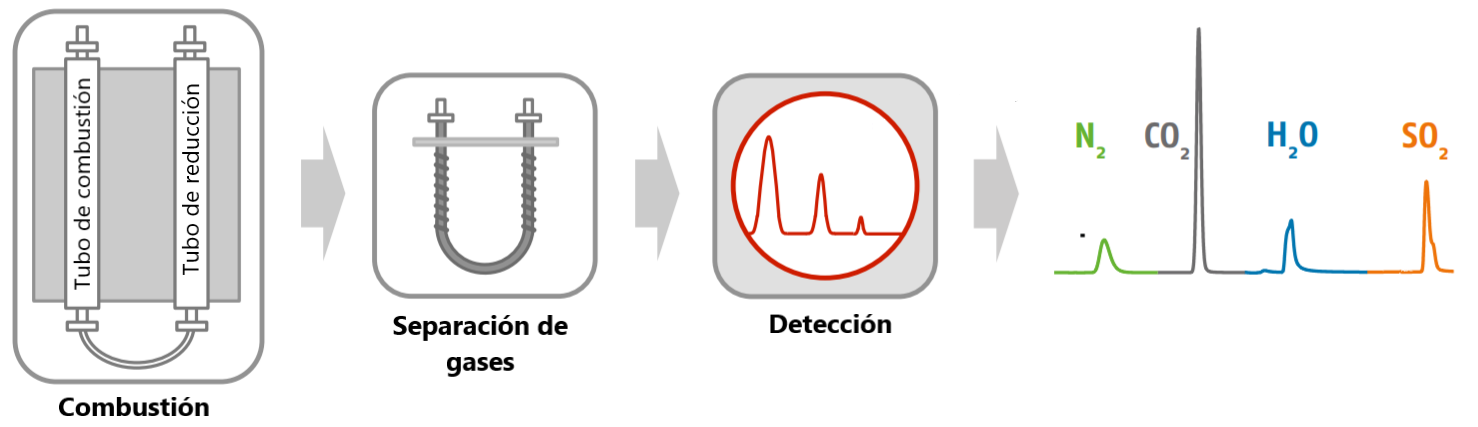
\includegraphics[width=0.9\textwidth]{Imagenes/C-N-Detection-2.png}
\caption{Procedimientos para el análisis elemental de carbono y nitrógeno: combustión, separación de gases y detección. Tomado de \textit{Flyer vario MICRO cube}, marca Elementar.}\label{Fig-CN-Esquema}
\end{figure}

\section{Simulaciones de Monte Carlo}\label{Secc-MonteCarlo}
Las simulaciones Monte Carlo son experimentos numéricos basados en variables de entrada con distribuciones de probabilidad establecidas y el modelo $z$ a explorar. En cada uno de los $N$ experimentos numéricos, los valores de las variables de entrada $x_i$, $1 \leq i \leq N$, se determina de acuerdo a sus distribuciones de probabilidades y los resultados son calculados mediante las relaciones del modelo $z = z(x_i)$ \cite{cruse1997reliability}. 
\\ \\ 
Las variables $x_i$ son variables aleatorias que adquieren un valor de un intervalo, finito o infinito, y siguen una función de densidad de probabilidad. Las funciones de densidad de probabilidad usuales son i) uniforme o rectangular, ii) exponencial, y iii) Gausiana. Típicamente, los resultados del modelo $z$ se expresan en términos de la media $\overline{z}$ y la varianza $\sigma^2(z)$, \cite{dunn2011exploring}
\begin{equation}
\overline{z} = \dfrac{1}{N}\sum_{i=1}^N z(x_i), \hspace{1cm} \sigma^2(z) = \dfrac{1}{N-1}\sum_{i=1}^N  (z(x_i) - \overline{z})^2.
\end{equation}
Según la ley de número grandes, si existen el valor medio y la desviación estándar, el valor promedio del modelo Monte Carlo tiende al valor real con el número de simulaciones $N\rightarrow \infty$, usualmente $N \sim 10^4$. 
\section{Hipótesis}\label{Sec-Hipotesis}
El fechado de núcleos sedimentarios con el radionúclido \PbCero\, requiere un conocimiento lo más aproximado posible de la actividad real de la muestra, la cual depende de la composición elemental de cada sección del núcleo sedimentario. El conocimiento de la composición elemental de cada sección permite conocer mejor la actividad real de cada muestra y obtener un fechado con \PbCero\, de mayor calidad. 
\section{Objetivos}\label{Sec-Objetivos}
El objetivo general de esta tesis es mejorar la cuantificación de los radionúclidos utilizados en el fechado de sedimentos recientes (\PbCero\, y \PbCuatro) a través de correcciones de densidad y autoabsorción específicas para cada muestra analizada. 
	\subsection{Objetivos específicos}\label{Sec-ObjEspec}
\begin{itemize}
\item Caracterizar los detectores de germanio hiper-puro tipo pozo utilizados en el LGIG: fondos, calibración de canal-energía y eficiencia-energía.
\item Seleccionar núcleos sedimentarios representativos de diversos sistemas acuáticos mexicanos. 
\item Determinar la composición elemental de algunas secciones de los núcleos  seleccionados y proponer su composición completa. 
\item Desarrollar códigos de programación para la lectura e integración de los datos provenientes de los equipos XRF y C-N, así como para ejecutar de manera sistemática el software ANGLE.
\item Estudiar los efectos de la densidad y composición elemental sobre la eficiencia de sistemas de espectrometría de rayos gammacon configuración de pozo para energías de 46.54 keV y 351.93 keV.
\item Estudiar el efecto de las correcciones realizadas en las actividades y el fechado de los núcleos seleccionados en relación a los resultados utilizando una composición de referencia (agua, composición química H$_2$O, densidad $\rho = 1$ g cm$^{-3}$). 
\end{itemize}

\chapter{Metodología}
\lettrine{E}{}l trabajo analítico de este proyecto de investigación se realizó en el Laboratorio de Geoquímica Isotópica y Geocronología (LGIG) del Instituto de Ciencias del Mar y Limnología, Universidad Nacional Autónoma de México - Unidad Académica Mazatlán, Sinaloa, México. El LGIG cuenta con sistemas de espectrometría de rayos gamma (Sección \ref{Secc-EspectrometriaGamma}), XRF (Sección \ref{Secc-EspectrometriaXRF}) y analizador elemental de carbono - nitrógeno, C-N (Sección \ref{Secc-CN})  que permiten obtener información sobre la composición elemental y la actividad de diversos radionúclidos (Tabla \ref{Table-MaterialesRef}). 
\\
\\
Los análisis elementales mediante XRF y C-N permiten proponer un método para estimar el 100 \% de la composición elemental de los sedimentos (Sección \ref{Secc-100Composicion}). Esta información, junto con la densidad de la muestra, permite corregir la actividad medida de las muestras utilizando el software ANGLE, Sección \ref{SubSec-ANGLE}.
\\
\\
El proyecto se centró en seis núcleos sedimentarios, pertenecientes a ecosistemas acuáticos de México: un lago cráter, el Golfo de México, el mar Caribe y el océano Pacífico (Sección \ref{Secc-ZonasSeleccionadas}). En la Sección \ref{Secc-Codigos} se describen los códigos de programación desarrollados para la lectura de  los datos experimentales y el cálculo sistemático de la eficiencia mediante ANGLE.
	\section{Sistemas de espectrometría de rayos gamma}\label{Secc-EspectrometriaGamma}
El LGIG posee cuatro sistemas de espectrometría de rayos gamma idenfiticados como G1, G2, G3 y G4. Cada sistema está compuesto por un detector de Ge hiper-puro en configuración tipo pozo (Sección \ref{SubSecc-DetecGe}), un blindaje pasivo (Sección \ref{SubSec-Blindaje}), un sistema de refrigeración (sección \ref{SubSec-Refrigeracion}) y electrónica asociada (Sección \ref{SubSec-Electronica}).
\\ 
\\ 
Cada sistema de espectrometría de rayos gamma se caracteriza por el espectro de fondo (Sección \ref{SubSec-Fondos}) y las calibraciones: canal - energía, eficiencia - energía. Para realizar y comprobar estas calibraciones se utilizaron una solución patrón de emisores gamma, un material de referencia Uranio - Torio ORE DL1a y Materiales de Referencia Certificados (Sección \ref{SubSec-MaterialesDeReferencia}). Las calibraciones se presentan en la Sección \ref{SubSec-CaliChannel}. 
\\
\\
El análisis de los espectros energéticos de rayos gamma se realizó mediante el software \textit{GammaVision}, versión 7.02.01, marca ORTEC. La sección \ref{SubSec-GammaVision} muestra las características y los ajustes utilizados en GammaVision. 
		\subsection[Detectores de Ge hiper-puro]{Detector de Ge hiper-puro en configuración tipo pozo}\label{SubSecc-DetecGe}
Los detectores de germanio hiper-puro son de tipo pozo y marca ORTEC. Las características principales, los parámetros geométricos necesarios para determinar la eficiencia mediante ANGLE y el modelo de cada detector se presentan en la Figura \ref{Fig-DetectorGeEsquema} y en la Tabla \ref{Tabla-Dimensiones-Detectores}. Todos los detectores tienen una profundidad de 40 mm y un diámetro de pozo efectivo de 15.5 mm.
\begin{figure}[h]
\centering
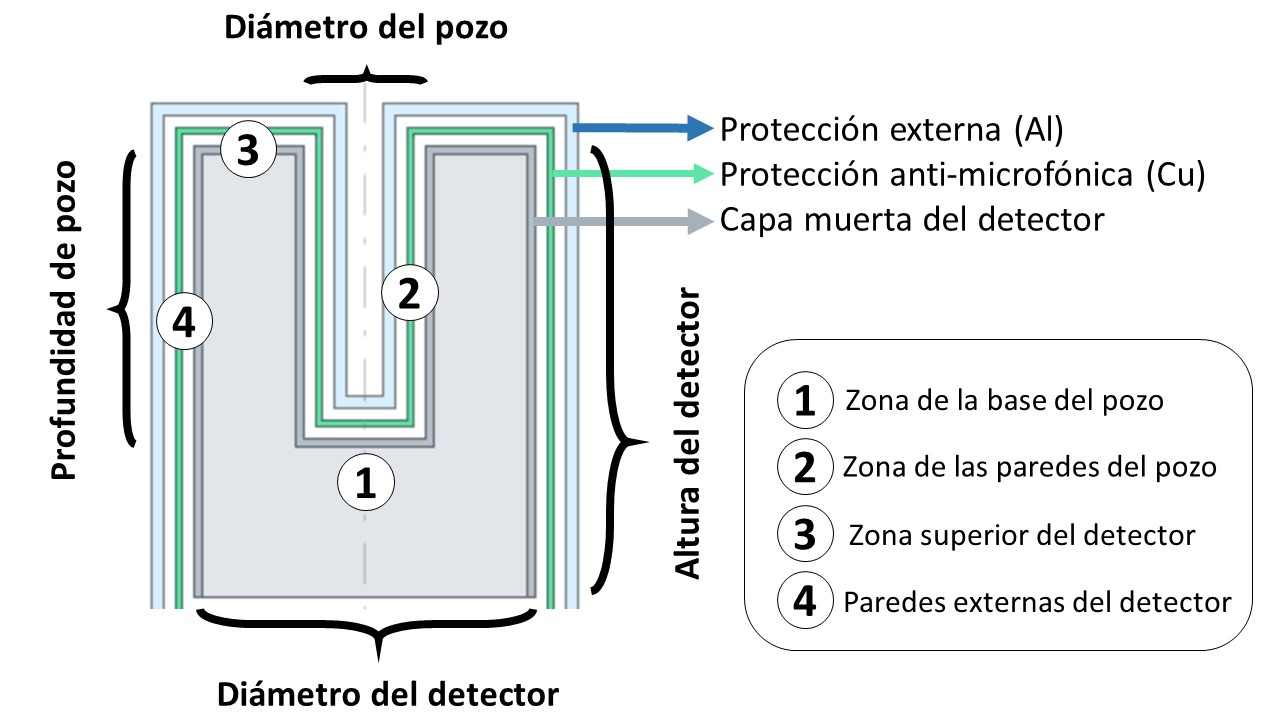
\includegraphics[width=\textwidth]{Imagenes/Zona_Detector_Ge.jpg}
\caption{Variables y zonas necesarias para especificar las dimensiones de los detectores de Ge hiper-puro en configuración pozo del LGIG.}\label{Fig-DetectorGeEsquema}
\end{figure}
\begin{table}
\caption{Características principales de los detectores de germanio hiper-puro en configuración tipo pozo. Las variables y zonas se detallan en la Figura \ref{Fig-DetectorGeEsquema}.}\label{Tabla-Dimensiones-Detectores}
\centering
\begin{tabular}{|c|c|c|c|c|c|}\hline
\rowcolor{Blue3}		&	Unidades	&	G1	&	G2	&	G3	&	G4	\\	\hline	\hline
\rowcolor{Blue2}	\multicolumn{2}{|c}{Dimensiones del cristal de Ge }			&		&		&		&		\\	\hline	
\rowcolor{Blue1}	Altura del detector	&	mm	&	64.8	&	66.5	&	69.7	&	69.1	\\		
\rowcolor{Blue1}	Diámetro del detector	&	mm	&	54.6	&	54.6	&	66.7	&	61.6	\\		
\rowcolor{Blue1}	Profundidad de pozo 	&	mm	&	55.6	&	53.5	&	56.7	&	55.1	\\		
\rowcolor{Blue1}	Diámetro de pozo 	&	mm	&	11.4	&	10.55	&	10.5	&	10.95	\\		
\rowcolor{Blue1}	Volumen activo	&	cc	&	124	&	124	&	206	&	169	\\	\hline	\hline
\rowcolor{Blue2}	\multicolumn{2}{|c}{Capa muerta de Ge }			&		&		&		&		\\	\hline	
\rowcolor{Blue1}	Zona 1	&	mm	&	$3\times 10^{-5}$	&	$3\times 10^{-5}$	&	$3\times 10^{-5}$	&	$3\times 10^{-5}$	\\		
\rowcolor{Blue1}	Zona 2	&	mm	&	$3\times 10^{-5}$	&	$3\times 10^{-5}$	&	$3\times 10^{-5}$	&	$3\times 10^{-5}$	\\		
\rowcolor{Blue1}	Zona 3	&	mm	&	0	&	$3\times 10^{-5}$	&	0	&	0	\\		
\rowcolor{Blue1}	Zona 4	&	mm	&	0.7	&	0.7	&	0	&	0.7	\\	\hline	\hline
\rowcolor{Blue2}	\multicolumn{2}{|c}{Protección anti-microfónica (Cu)}			&		&		&		&		\\	\hline	
\rowcolor{Blue1}	Zona 3	&	mm	&	1.6	&	1.6	&	1.6	&	1.6	\\	\hline	\hline
\rowcolor{Blue2}	\multicolumn{2}{|c}{Protección externa (Al)}			&		&		&		&		\\	\hline	
\rowcolor{Blue1}	Zona 1	&	mm	&	1	&	1	&	1	&	2.032	\\		
\rowcolor{Blue1}	Zona 2	&	mm	&	0.5	&	0.5	&	0.5	&	0.5	\\		
\rowcolor{Blue1}	Zona 3	&	mm	&	2.032	&	2.032	&		&	2.032	\\	\hline	\hline
\rowcolor{Blue2}	\multicolumn{2}{|c}{Distancia entre Al y Cu}			&		&		&		&		\\	\hline	
\rowcolor{Blue1}	Zona 1	&	mm	&	7.8	&	3.125	&	7.92	&	3.9	\\		
\rowcolor{Blue1}	Zona 2	&	mm	&	1.8	&	1.15	&	1.3	&	1.3	\\		
\rowcolor{Blue1}	Zona 3	&	mm	&	6.4	&	8.4	&	4.2	&	8.39	\\	\hline	\hline
\rowcolor{Blue2}	\multicolumn{2}{|c}{Distancia entre Cu y Ge}			&		&		&		&		\\	\hline	
\rowcolor{Blue1}	Zona 1	&	mm	&	7.8	&	3.125	&	7.92	&	3.99	\\		
\rowcolor{Blue1}	Zona 2	&	mm	&	1.8	&	1.15	&	1.3	&	1.3	\\		
\rowcolor{Blue1}	Zona 3	&	mm	&	0.2	&	0.279	&	4.2	&	0.279	\\	\hline	\hline
\rowcolor{Blue2}	Voltaje operativo	&	V	&	+2500	&	+2500	&	+1500	&	+3600	\\	\hline	\hline
\rowcolor{Blue1} Modelo & GWL- & 120-15-5 & 120-15-LB-AWT & \multicolumn{2}{c|}{150-15-LB-AWT}\\ \hline
\end{tabular}
\begin{flushleft}
Zona 1: parte inferior del pozo. \\
Zona 2: lateral del pozo.  \\
Zona 3: parte superior del detector. \\
Zona 4: parte lateral externa del detector.
\end{flushleft}
\end{table}
		\subsection{Blindaje de la radiación}\label{SubSec-Blindaje}
Los detectores de Ge hiper-puro del LGIG cuentan con blindaje pasivo (HPLBS - High Performance Low Background Lead Shields, ORTEC). El blindaje es cilíndrico, con $\sim$ 10 cm  de plomo de bajo fondo, y dos capas de Cu y Sn para la absorción de los rayos X generados en el blindaje de plomo \cite{OrtecShield}. La parte inferior del blindaje contiene una apertura circular por donde se comunica el detector con el sistema de refrigeración y la electrónica asociada.		
		\subsection{Sistema de refrigeración}\label{SubSec-Refrigeracion}
Cada sistema de espectrometría de rayos gamma se refrigera con un sistema de condensación de nitrógeno líquido (MÖBIUS Recycler, ORTEC), constituido por un dewar, un sistema de presión de vapor y un condensador criogénico que reutiliza el nitrógeno manteniendo la presión de vapor constante a 3.5 kPa \cite{Mobius}. La capacidad de almacenamiento de nitrógeno líquido es de 28 L y requiere ser rellenado aproximadamente una vez al año, dadas las condiciones ambientales de Mazatlán, Sinaloa, México.
		\subsection{Electrónica asociada}\label{SubSec-Electronica}
Cada detector cuenta en su base con un preamplificador que recibe la carga creada por la interacción de los rayos gamma de la muestra y el cristal de Ge. La señal es transmitida a la electrónica integrada \textit{DSPEC jr 2.0} (ORTEC), que integra una fuente de tensión de alto voltaje, un amplificador, un analizador multicanal y un convertidor análogo - digital (ADC).
\\
\\
En la  Figura \ref{Fig-G1System} se aprecian el sistema de refrigeración, el blindaje, el recubrimiento externo del cristal de Ge hiper-puro (Cu y Al) y el recubrimiento interior del sistema de blindaje (Cu).
\begin{figure}[h]
\centering
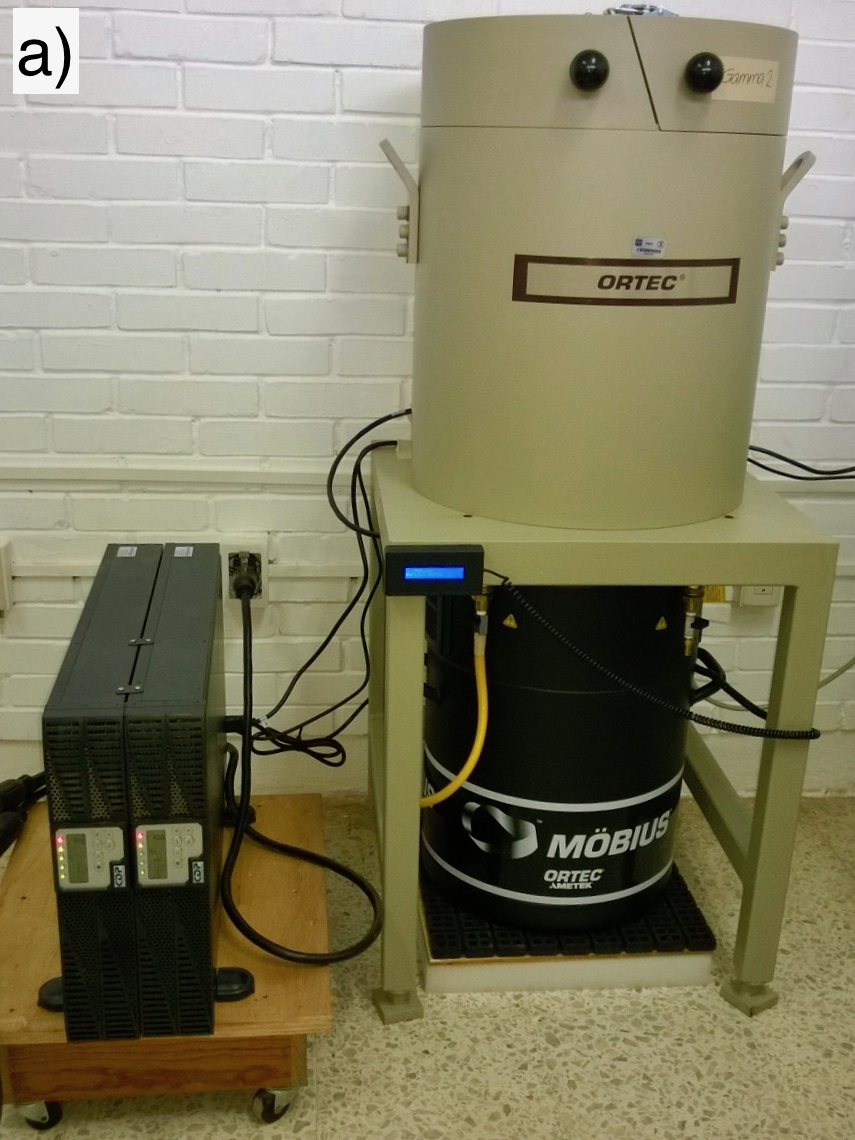
\includegraphics[height=0.4\textheight]{Imagenes/GammaSystem.jpg}
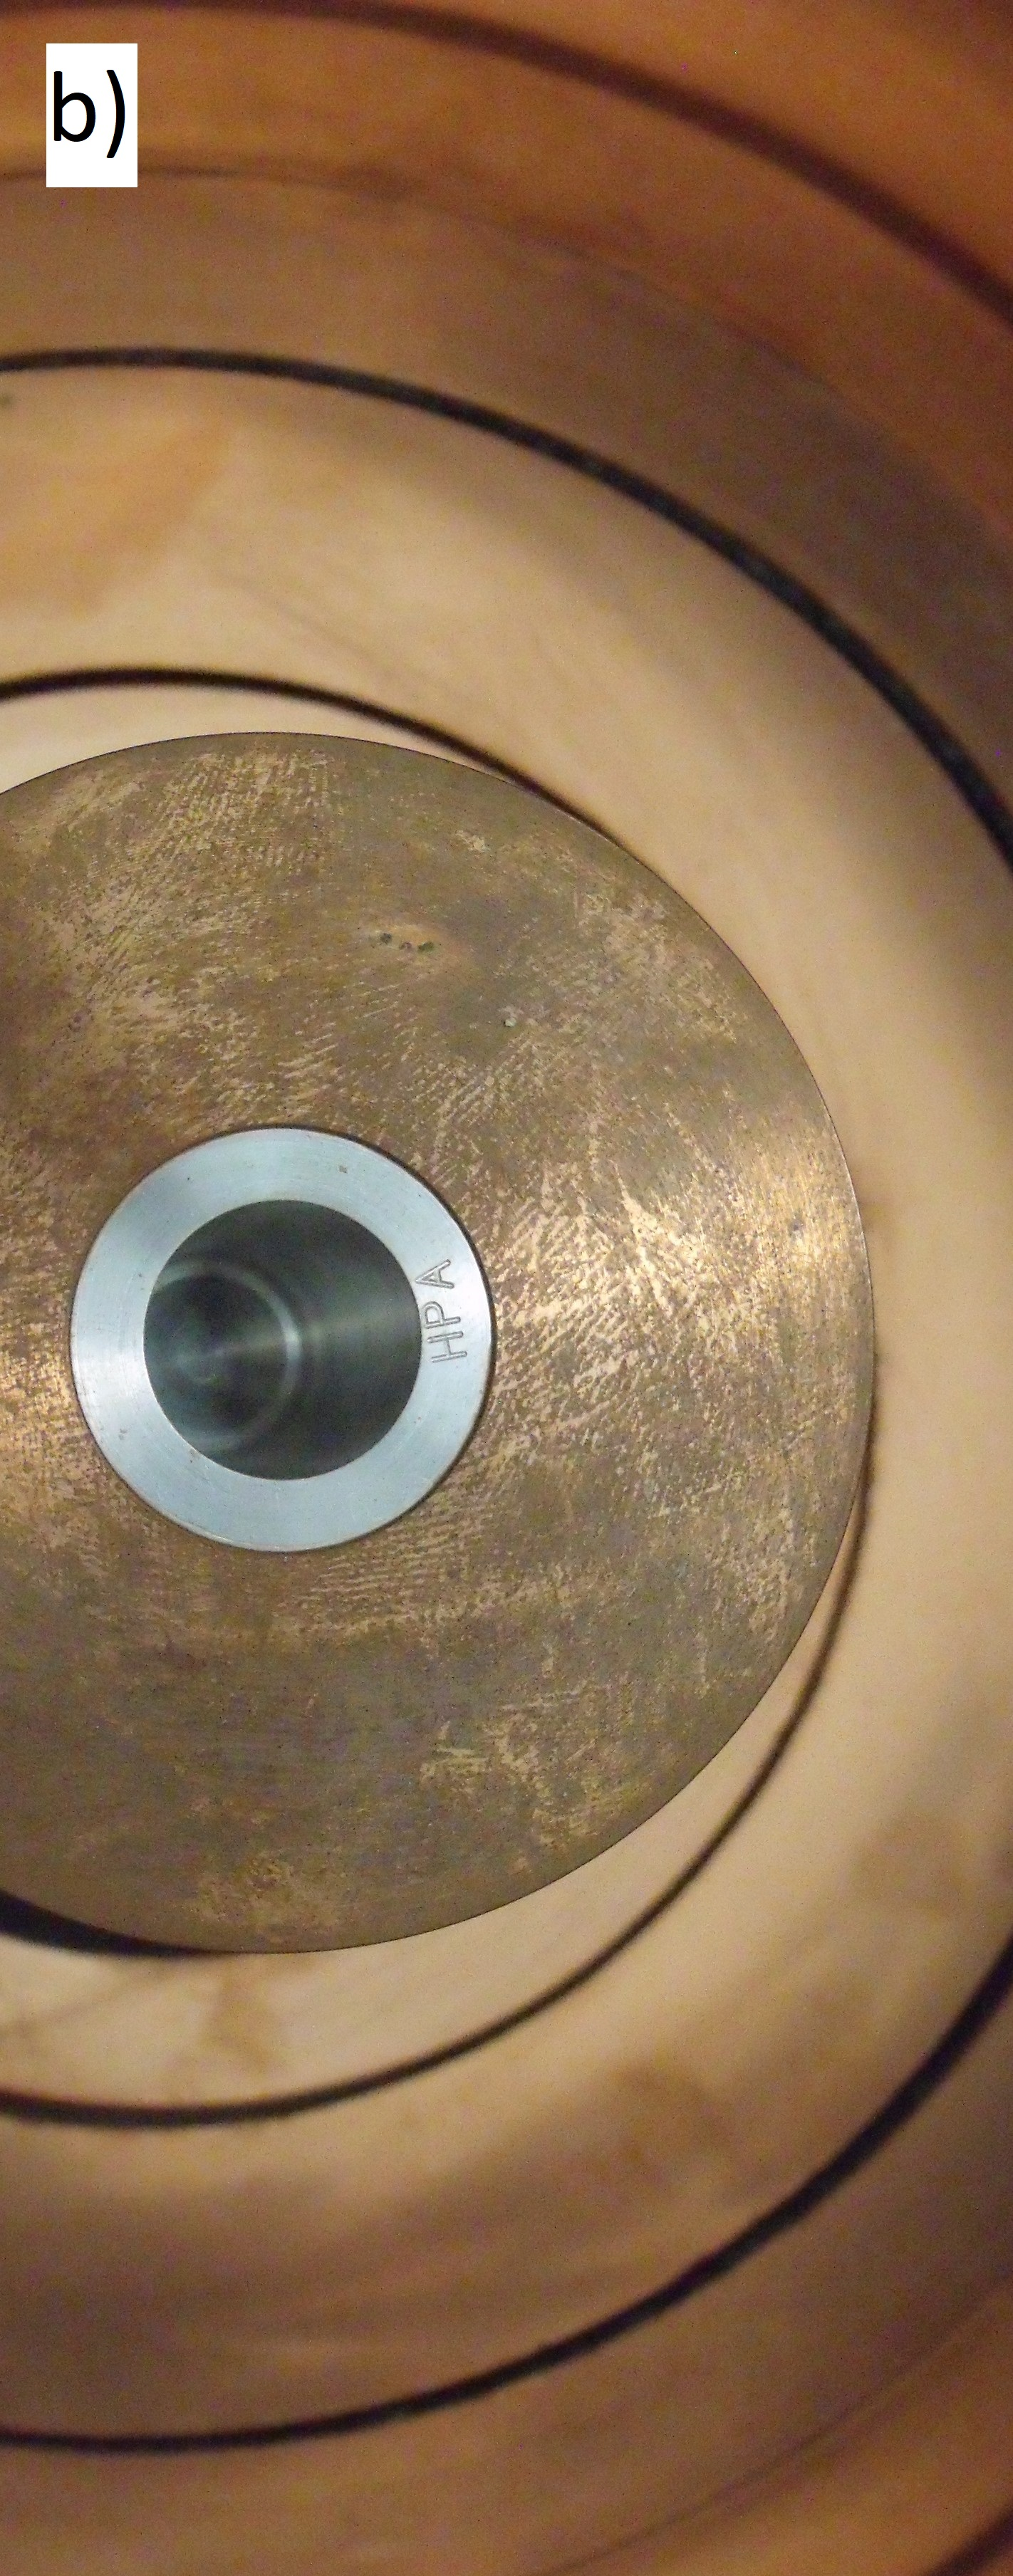
\includegraphics[height=0.4\textheight]{Imagenes/DSCF1886.jpg}
\caption{Sistema de espectrometría de rayos gamma G2 del LGIG. a) Sistema de refrigeración, blindaje y fuente de alimentación. b) Detector de Ge hiper-puro dentro de blindaje.}\label{Fig-G1System}
\end{figure}
		\subsection{Espectro del fondo}\label{SubSec-Fondos}
El espectro de fondo de cada sistema de espectrometría de rayos gamma del LGIG es medido durante aproximadamente dos semanas. En general, se pueden observar radionúclidos antropogénicos ($^{60}$Co y $^{137}$Cs), primordiales ($^{235}$U, $^{238}$U, $^{232}$Th, $^{40}$K) y de rayos cósmicos, entre otros \cite{gilmore2008}. Cada espectro medido debe ser corregido con el espectro de fondo correspondiente. 
\\
\\
En los espectros de fondos de los sistemas de espectrometría gamma del LGIG (Figura \ref{Fig-Fondos}) se observa claramente los radionúclidos primordiales \Kcuarenta, \PbCuatro\, y \BiCuatro, descendientes de \UDosTresOcho\, (Figura \ref{Fig-SerieUranio}). El mayor fondo del detector G1 es debido a que no se trata de un detector con configuración de bajo fondo, y el mayor fondo de los detectores G3 y G4 es debido a su mayor volumen activo. 
\\
\\
La Tabla \ref{Table-CuentasBackground} muestra el número de cuentas del fondo para cada uno de los sistemas de espectrometría de rayos gamma en las energías de interés. El tiempo muerto de la detección de rayos gammas es, en la mayoría de los casos, inferior al 1 \% debido a la baja actividad de las muestras ambientales analizadas en el presente trabajo. Por lo anterior, también se espera que el efecto de \textit{pile-up} sea despreciable y en todo caso, corregido por el sistema electrónico \textit{DSPEC jr 2.0} (ORTEC). 
\begin{figure}[h]
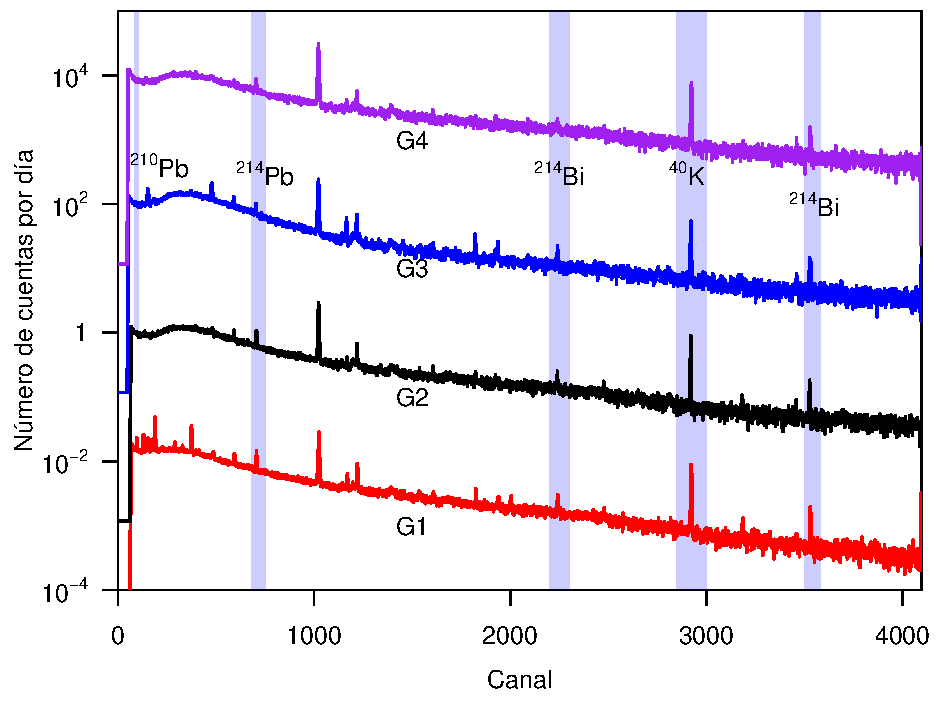
\includegraphics[width=0.9\textwidth]{Imagenes/Fondos.pdf}
\caption{Espectro del fondo para los sistemas de espectrometría de rayos gamma del LGIG.}\label{Fig-Fondos}
\end{figure}
\begin{table}[h]
\centering
\caption{Tasa de cuentas del espectro de fondo para las energías de interés y para cada uno de los sistemas de espectrometría de rayos gamma del LGIG.}\label{Table-CuentasBackground}
\begin{tabular}{|c|c|c|c|c|c|}
	\hline												
\rowcolor{Blue2}	Energía 	&	Radionúclido 	&	G1	&	G2	&	G3	&	G4	\\	\hline
	keV	&		&	 \multicolumn{4}{c|}{Número de cuentas por segundo}           							\\	\hline
\rowcolor{Blue1}	46.54	&	$^{210}$Pb	&	0.003	&	0	&	0	&	0	\\	
\rowcolor{Blue1}	351.99	&	$^{214}$Pb	&	0.003	&	0.001	&	0.004	&	0.001	\\	\hline
\end{tabular}
\end{table}
		\subsection{Materiales de Referencia Certificados}\label{SubSec-MaterialesDeReferencia}
El LGIG cuenta con materiales de referencia utilizados para realizar y comprobar las calibraciones de energía y eficiencia. Se utiliza una solución acuosa patrón de emisores gamma y un material de referencia Uranio - Torio ORE DL1a para realizar las calibraciones en eficiencia y energía. En la Tabla \ref{Table-MaterialesRef} se muestran las características de esta solución y de otros radionúclidos de interés para el LGIG. Por otra parte, la validación de las calibraciones se realiza con Materiales de Referencia Certificados que se muestran en la Tabla \ref{Table-OtrosMaterialesRefIAEA}.
\begin{table}[h]
\centering
\caption{Características de los radionúclidos del material de referencia Mix-Gamma y otros radionúclidos de interés para el LGIG (con $^{*}$): núcleo progenitor y núcleo descendiente, proceso nuclear de desintegración o des-excitación y energía del rayo gamma emitido.}\label{Table-MaterialesRef}
\begin{tabular}{|c|c|c|c|c|c|c|}
\hline																
\rowcolor{Blue3}		\begin{tabular}{@{}c@{}}Núcleo \\ progenitor \end{tabular}	&	$T_{\frac{1}{2}}$       	&	\begin{tabular}{@{}c@{}}Proceso \\ nuclear \end{tabular}	&	\begin{tabular}{@{}c@{}}Núcleo \\ descendiente \end{tabular}	&	 \multicolumn{2}{|c|}{\begin{tabular}{@{}c@{}} Energía del estado \\ inicial y final  \end{tabular} }           			&	\begin{tabular}{@{}c@{}}Energía\\ de rayo \\ gamma \end{tabular}	\\ 	\hline
			&		&		&		&	keV	&	keV	&	keV	\\ 	\hline
\rowcolor{Blue2}		 \multicolumn{7}{|c|}{Mix-Gamma}           													\\ 	\hline
\rowcolor{Blue1}	\cellcolor{Green3}	$^{241}$Am$^{*}$	&	432.6 años	&	$\alpha$	&	 	$^{237}$Np	 	&	 	59.54	 	&	 	0	 	&	\cellcolor{Green3} 59.54	\\ 	
\rowcolor{Blue1}		 	$^{109}$Cd	 	&	 	461.9 días 	 	&	C. E.	&	 	$^{109}$Ag	 	&	 	88.04	 	&	 	0	 	&	88.04	\\ 	
\rowcolor{Blue1}		 	$^{57}$Co	 	&	 	271.8 días	 	&	C. E.	&	 	$^{57}$Fe	 	&	 	136.47	 	&	 	14.41	 	&	122.06	\\ 	
\rowcolor{Blue1}		 	$^{139}$Ce	 	&	 	137.6 días	 	&	C. E.	&	 	$^{139}$La	 	&	 	165.86	 	&	 	0	 	&	165.86	\\ 	
\rowcolor{Blue1}		 	$^{203}$Hg	 	&	 	46.59 días	 	&	$\beta^-$	&	 	$^{203}$Tl	 	&	 	279.19	 	&	 	0	 	&	279.19	\\ 	
\rowcolor{Blue1}		 	$^{113}$Sn	 	&	 	115.1 días	 	&	C. E.	&	 	$^{113}$In	 	&	 	391.69	 	&	 	0	 	&	391.69	\\ 	
\rowcolor{Blue1}		 	$^{134}$Ba	 	&	 		 	&	$\gamma$	&	 	$^{134}$Ba	 	&	 	604.7	 	&	 	0	 	&	604.7	\\ 	
\rowcolor{Blue1}	\cellcolor{Green3}	 	$^{137}$Cs$^{*}$	 	&	 	30.05 años	 	&	$\beta^-$	&	 	$^{137}$Ba	 	&	 	667.66	 	&	 	0	 	&	\cellcolor{Green3} 661.66	\\ 	
\rowcolor{Blue1}	\cellcolor{Green3}	 	$^{134}$Cs	$^{*}$ 	&	 	2.064 años	 	&	$\beta^-$	&	 	$^{134}$Ba	 	&	 	1400.59	 	&	 	604.7	 	&	\cellcolor{Green3} 795.9	\\ 	
\rowcolor{Blue1}		 	$^{54}$Mn	 	&	 	312.2 días	 	&	C. E.	&	 	$^{54}$Cr	 	&	 	834.8	 	&	 	0	 	&	834.8	\\ 	
\rowcolor{Blue1}		 	$^{88}$Y	 	&	 	106.6 días	 	&	C. E.	&	 	$^{88}$Sr	 	&	 	2734.1	 	&	 	1836.1	 	&	989	\\ 	
\rowcolor{Blue1}		 	$^{65}$Zn	 	&	 	244 días	 	&	C. E.	&	 	$^{65}$Cu	 	&	 	1115.5	 	&	 	0	 	&	1115.5	\\ 	
\rowcolor{Blue1}		 	$^{88}$Sr	 	&	 		 	&	$\gamma$	&	 	$^{88}$Sr	 	&	 	1836.1	 	&	 	0	 	&	1836	\\ 	\hline
\rowcolor{Blue2}		 \multicolumn{7}{|c|}{Radionúclidos de interés para el LGIG}           													\\ 	\hline
\rowcolor{Blue1}	\cellcolor{Green3}	$^{7}$Be	&	53.22 días 	&	C. E.	&	$^{7}$Li	&	477.6	&	0	&	\cellcolor{Green3} 477.6	\\ 	
\rowcolor{Blue1}	\cellcolor{Green3}	$^{208}$Tl	&	1.402 $\cdot 10^{10}$ años	&	$\beta^-$	&	$^{208}$Pb	&	3197.71	&	2614.55	&	\cellcolor{Green3} 583.16	\\ 	
\rowcolor{Blue1}	\cellcolor{Green3}	$^{228}$Ac	&	1.402 $\cdot 10^{10}$ años	&	$\beta^-$	&	$^{228}$Th	&	396.08	&	57.76	&	\cellcolor{Green3} 338.32	\\ 	
\rowcolor{Blue1}	\cellcolor{Green3}	$^{40}$K	&	1.25 $\cdot 10^{9}$ años	&	E. C. 	&	$^{40}$Ar	&	1460.851	&	0	&	\cellcolor{Green3} 1460.851	\\ 	
\rowcolor{Blue1}	\cellcolor{Green3}	$^{210}$Pb	&	22.23 años	&	$\beta^-$	&	$^{210}$Bi	&	46.54	&	0	&	\cellcolor{Green3} 46.54	\\ 	
\rowcolor{Blue1}	\cellcolor{Green3}	$^{214}$Pb	&	1600 años	&	$\beta^-$	&	$^{214}$Bi	&	351.93	&	0	&	\cellcolor{Green3} 351.93	\\ 	
\rowcolor{Blue1}	\cellcolor{Green3}	$^{234}$Th	&	4.468 $\cdot 10^{9}$ años	&	$\beta^-$	&	$^{234}$Pa	&	166.72	&	103.42	&	\cellcolor{Green3} 63.3	\\ 	\hline
\end{tabular}
\end{table}
\begin{table}[h]
\centering
\caption{Materiales de Referencia Certificados, MRC.}\label{Table-OtrosMaterialesRefIAEA}
\begin{tabular}{|c|c|}
	\hline								
\rowcolor{Blue2}	MRC	&	Radionúclidos	\\	\hline	
\rowcolor{Blue1}	IAEA 300	&		$^{40}$K, $^{60}$Co, $^{125}$Sb, $^{134}$Cs, $^{155}$Eu, $^{210}$Pb, $^{210}$Po, $^{228}$Ra, $^{234}$U, $^{239,240}$Pu, 	 $^{241}$Am. 	\\	\hline	
\rowcolor{Blue1}	IAEA 313	&	$^{226}$Ra, Th, U.				\\	\hline	
\rowcolor{Blue1}	IAEA 314	&	$^{226}$Ra, Th, U.				\\	\hline	
\rowcolor{Blue1}	IAEA 375	&		$^{40}$K, $^{90}$Sr, $^{106}$Ru, $^{125}$Sb, $^{129}$I, $^{134}$Cs, $^{137}$Cs, $^{226}$Ra, $^{232}$Th. 	\\	\hline	
\rowcolor{Blue1}	IAEA-384	&		\begin{tabular}{@{}c@{}}$^{40}$K, $^{60}$Co, $^{155}$Eu, $^{230}$Th, $^{238}$U,  	$^{238}$Pu, $^{239,2340}$Pu, $^{241}$Am, $^{90}$Sr, $^{137}$Cs,\\  	 $^{210}$Pb, $^{226, 228}$Ra, $^{232}$Th, $^{234, 235}$U, $^{239,240,241}$Pu. \end{tabular}	\\	\hline	
\rowcolor{Blue1}	IAEA-414	&		$^{40}$K, $^{137}$Cs, $^{232}$Th, $^{234,235,238}$U, $^{238, 239+240}$Pu,         	 $^{241}$Am, $^{90}$Sr, $^{210}$Pb, $^{226}$Ra, $^{239,240,241}$Pu.          	\\	\hline	
\rowcolor{Blue1}	IAEA-444	&		$^{54}$Mn, $^{60}$Co, $^{65}$Zn, $^{109}$Cd,      $^{134,137}$Cs, $^{210}$Pb, $^{241}$Am.  \\	\hline	
\rowcolor{Blue1}	IAEA-448	&		 $^{226}$Ra, $^{40}$K, $^{208}$Tl, $^{210, 212}$Pb,     $^{228}$Ac,  $^{232}$Th, $^{235, 238}$U.      \\	\hline	
\rowcolor{Blue1}	DL1a	&	U, Th, $^{226}$Ra, $^{210}$Pb.				\\	\hline	
\rowcolor{Blue1}	KCl	&	$^{40}$K.				\\	\hline	
\end{tabular}
\end{table}
		\subsection{Calibraciones}\label{SubSec-CaliChannel}
Las calibraciones se realizaron para cada detector y dos geometrías. El LGIG usa geometrías según la cantidad disponible de muestra, que se denotan 2 mL y 4 mL. En la Figura \ref{Fig-Cal-Canal-Energia} se observa que las calibraciones canal - energía presentaron una excelente linealidad. 
\\
\\
La Tabla \ref{Tabla-EficienciasPb} muestra los valores de la eficiencia de referencia para las dos energías de interés (46.54 keV y 351.93 keV), los diferentes sistemas de espectrometría (G1, G2, G3 y G4) y dos de las geometrías (2 mL y 4 mL) utilizadas en el LGIG. Una geometría de 2 mL denota un volumen de muestra de 1.939 $\pm$ 0.007 cm$^{3}$ y una geometría de 4 mL denota un volumen de muestra de 4.071 $\pm$ 0.004 cm$^{3}$. La Figura \ref{Fig-EficienciaAgua} muestra algunas curvas de eficiencia referencia (ver Objetivos específicos, Sección \ref{Sec-ObjEspec}) en cada detector y diferentes geometrías.
\\
\\
Para reducir la incertidumbre de la medida debida a la calibración y disponer de actividades lo más exactas posibles, las eficiencias fueron determinadas tan sólo para los radionúclidos de interés (Tabla \ref{Table-MaterialesRef}), por lo que no se propuso una curva de eficiencia continua ni se realizó correcciones debido a la coincidencia de dos rayos gamma asociados al mismo evento de decaimiento, (TCSC, por sus siglas en inglés). En caso de requerir la cuantificación de nuevos radionúclidos, sus eficiencias son determinadas por simulación mediante el software ANGLE (Sección \ref{SubSec-ANGLE}) utilizando puntos de calibración pertenecientes a emisores monoenergéticos y, por lo tanto, no afectadas por correcciones de coincidencia. 
\begin{table}[h]
\centering
\caption{Eficiencia de referencia para \PbCero\,(46.54 keV) y \PbCuatro\,(351.93 keV) de los diferentes sistemas gamma del LGIG para diferentes geometrías (2 mL y 4 mL).}\label{Tabla-EficienciasPb}
\begin{tabular}{|c|c|c|} \hline
\rowcolor{Blue2}	Detector y geometría & $\epsilon$(\PbCero) & $\epsilon$(\PbCuatro) \\ \hline
\rowcolor{Blue1}	G1 - 2 mL & 0.71 & 0.25 \\
\rowcolor{Blue1}	G1 - 4 mL & 0.63 & 0.22 \\
\rowcolor{Blue1}	G2 - 2 mL & 0.71 & 0.25 \\
\rowcolor{Blue1}	G2 - 4 mL & 0.68 & 0.24 \\
\rowcolor{Blue1}	G3 - 2 mL & 0.71 & 0.34 \\
\rowcolor{Blue1}	G3 - 4 mL & 0.64 & 0.30 \\
\rowcolor{Blue1}	G4 - 2 mL & 0.66 & 0.30 \\
\rowcolor{Blue1}	G4 - 4 mL & 0.63 & 0.28 \\ \hline
\end{tabular}
\end{table}
\begin{figure}[h]
\centering
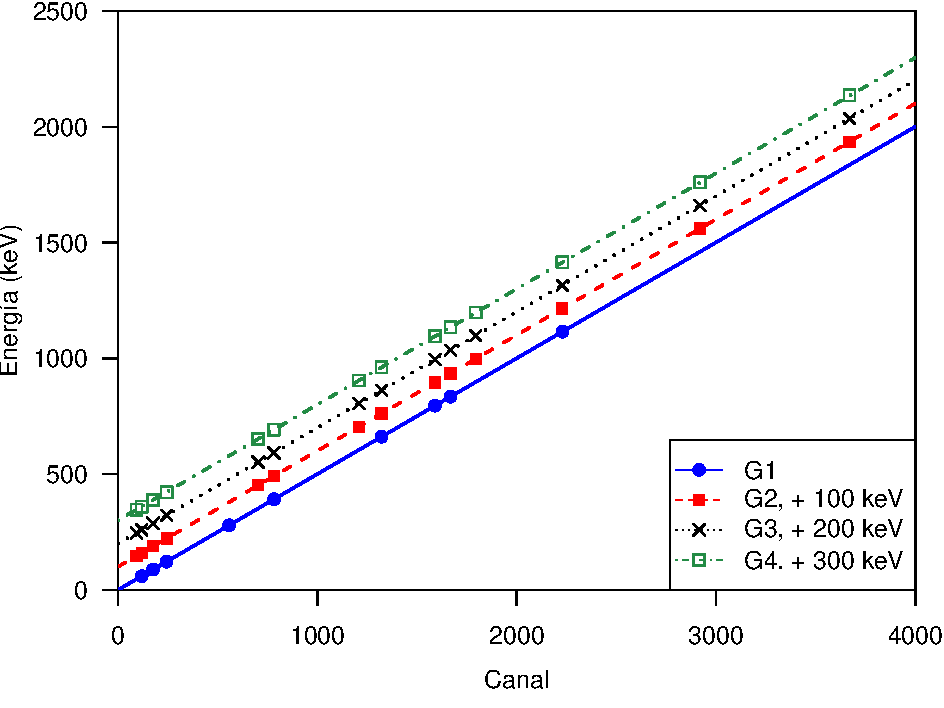
\includegraphics[width=0.7\textwidth]{Imagenes/Calibraciones_Canal_Energia.pdf}
\caption{Calibración canal-energía para los sistemas de espectrometría de rayos gamma del LGIG. Las calibraciones se encuentran desplazadas en + 100 keV, + 200 keV y +300 keV para G2, G3 y G4, respectivamente.}\label{Fig-Cal-Canal-Energia}
\end{figure}
\begin{figure}[h]
\centering
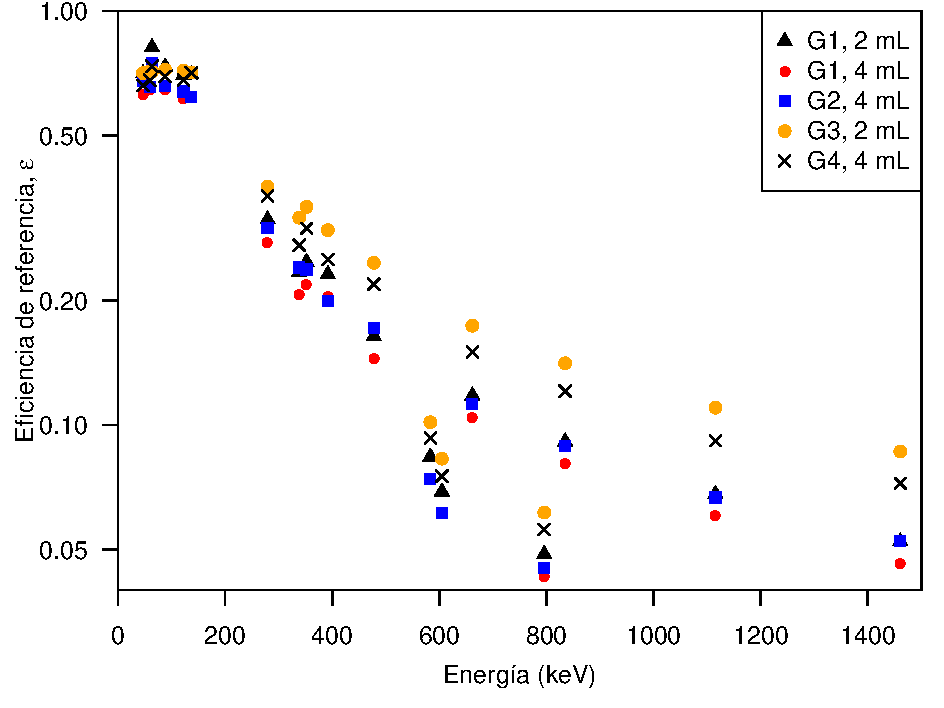
\includegraphics[width=0.7\textwidth]{Imagenes/Eficiencia_agua.pdf}
\caption{Eficiencia de referencia para diferentes detectores y geometrías (2 mL y 4 mL) del LGIG.}\label{Fig-EficienciaAgua}
\end{figure}
		\subsection{GammaVision}\label{SubSec-GammaVision}
El control de la electrónica y el análisis de los espectros energéticos de rayos gamma se realizó mediante el software GammaVision (ORTEC). La búsqueda y el análisis de los fotopicos de interés, y el cálculo de la actividad específica (Bq kg$^{-1}$), se efectuó con base en:
\begin{itemize}
\item Las calibraciones en energía y en eficiencia. 
\item El espectro del fondo.
\item La librería con información nuclear de los radioisótopos de interés. 
\end{itemize}
Algunos parámetros utilizados en el análisis son: \cite{GammaVisionManual}
\begin{itemize}
\item Background type: 3-Point. El cálculo del fondo para un pico se realiza como el promedio del fondo de lado izquierdo (bajas energías) y derecho (altas energías) del centroide de un fotopico. El fondo izquierdo/derecho es definido como el valor mínimo del promedio de tres canales en el intervalo que comprende el canal del centroide $\pm 4\times$ FWHM.
\item MDA Type: Traditional ORTEC. La actividad mínima detectable (MDA) es la estimación de la actividad que, \textit{a priori}, puede proporcionar cada sistema de detección. Su valor depende de la eficiencia, fondo y tiempo de medida. 
\item Peak search sensitivity: 3. La sensibilidad en la búsqueda de picos (entre 1 y 5) permite seleccionar la importancia de los picos que se consideran en el análisis. Un valor bajo (1) puede encontrar muchos picos “falsos” y el valor más alto (5) puede ignorar picos relevantes. 
\item Analysis method: ROI32. El método ROI32 busca picos tan sólo en las zonas de interés (ROI) basándose en la calibración canal – energía. 
\end{itemize} 
\newpage
\newpage
	\section{Espectrometría de fluorescencia de rayos X}\label{Secc-EspectrometriaXRF}
En el LGIG se mide la concentración elemental para $Z>10$ a través de la técnica XRF (Sección \ref{SubSec-XRF-Intro}) mediante el equipo \textit{SPECTRO XEPOS III}. El equipo de medición se muestra en la Figura \ref{Fig-XEPOS}. La cantidad de masa requerida es de 2 a 4 g. La incertidumbre asociada a la medida de la concentración $x_i$ de elemento $i$, $\bigtriangleup x_i$, se calcula utilizando una carta de calidad mediante la relación entre la desviación estándar $\sigma_\text{Referencia}$ y el valor promedio $\overline{x}_\text{Referencia}$ para diferentes mediciones de Materiales de Referencia Certificados. Si $x_i$ es el valor medido de un elemento $i$, entonces la incertidumbre asociada, $\bigtriangleup x_i$, es
\begin{equation}\label{Eq-SigmaRef}
\bigtriangleup x_i = \dfrac{\sigma_\text{Referencia}}{\overline{x}_\text{Referencia}}\times x_i.
\end{equation}
\begin{figure}[h]
\centering
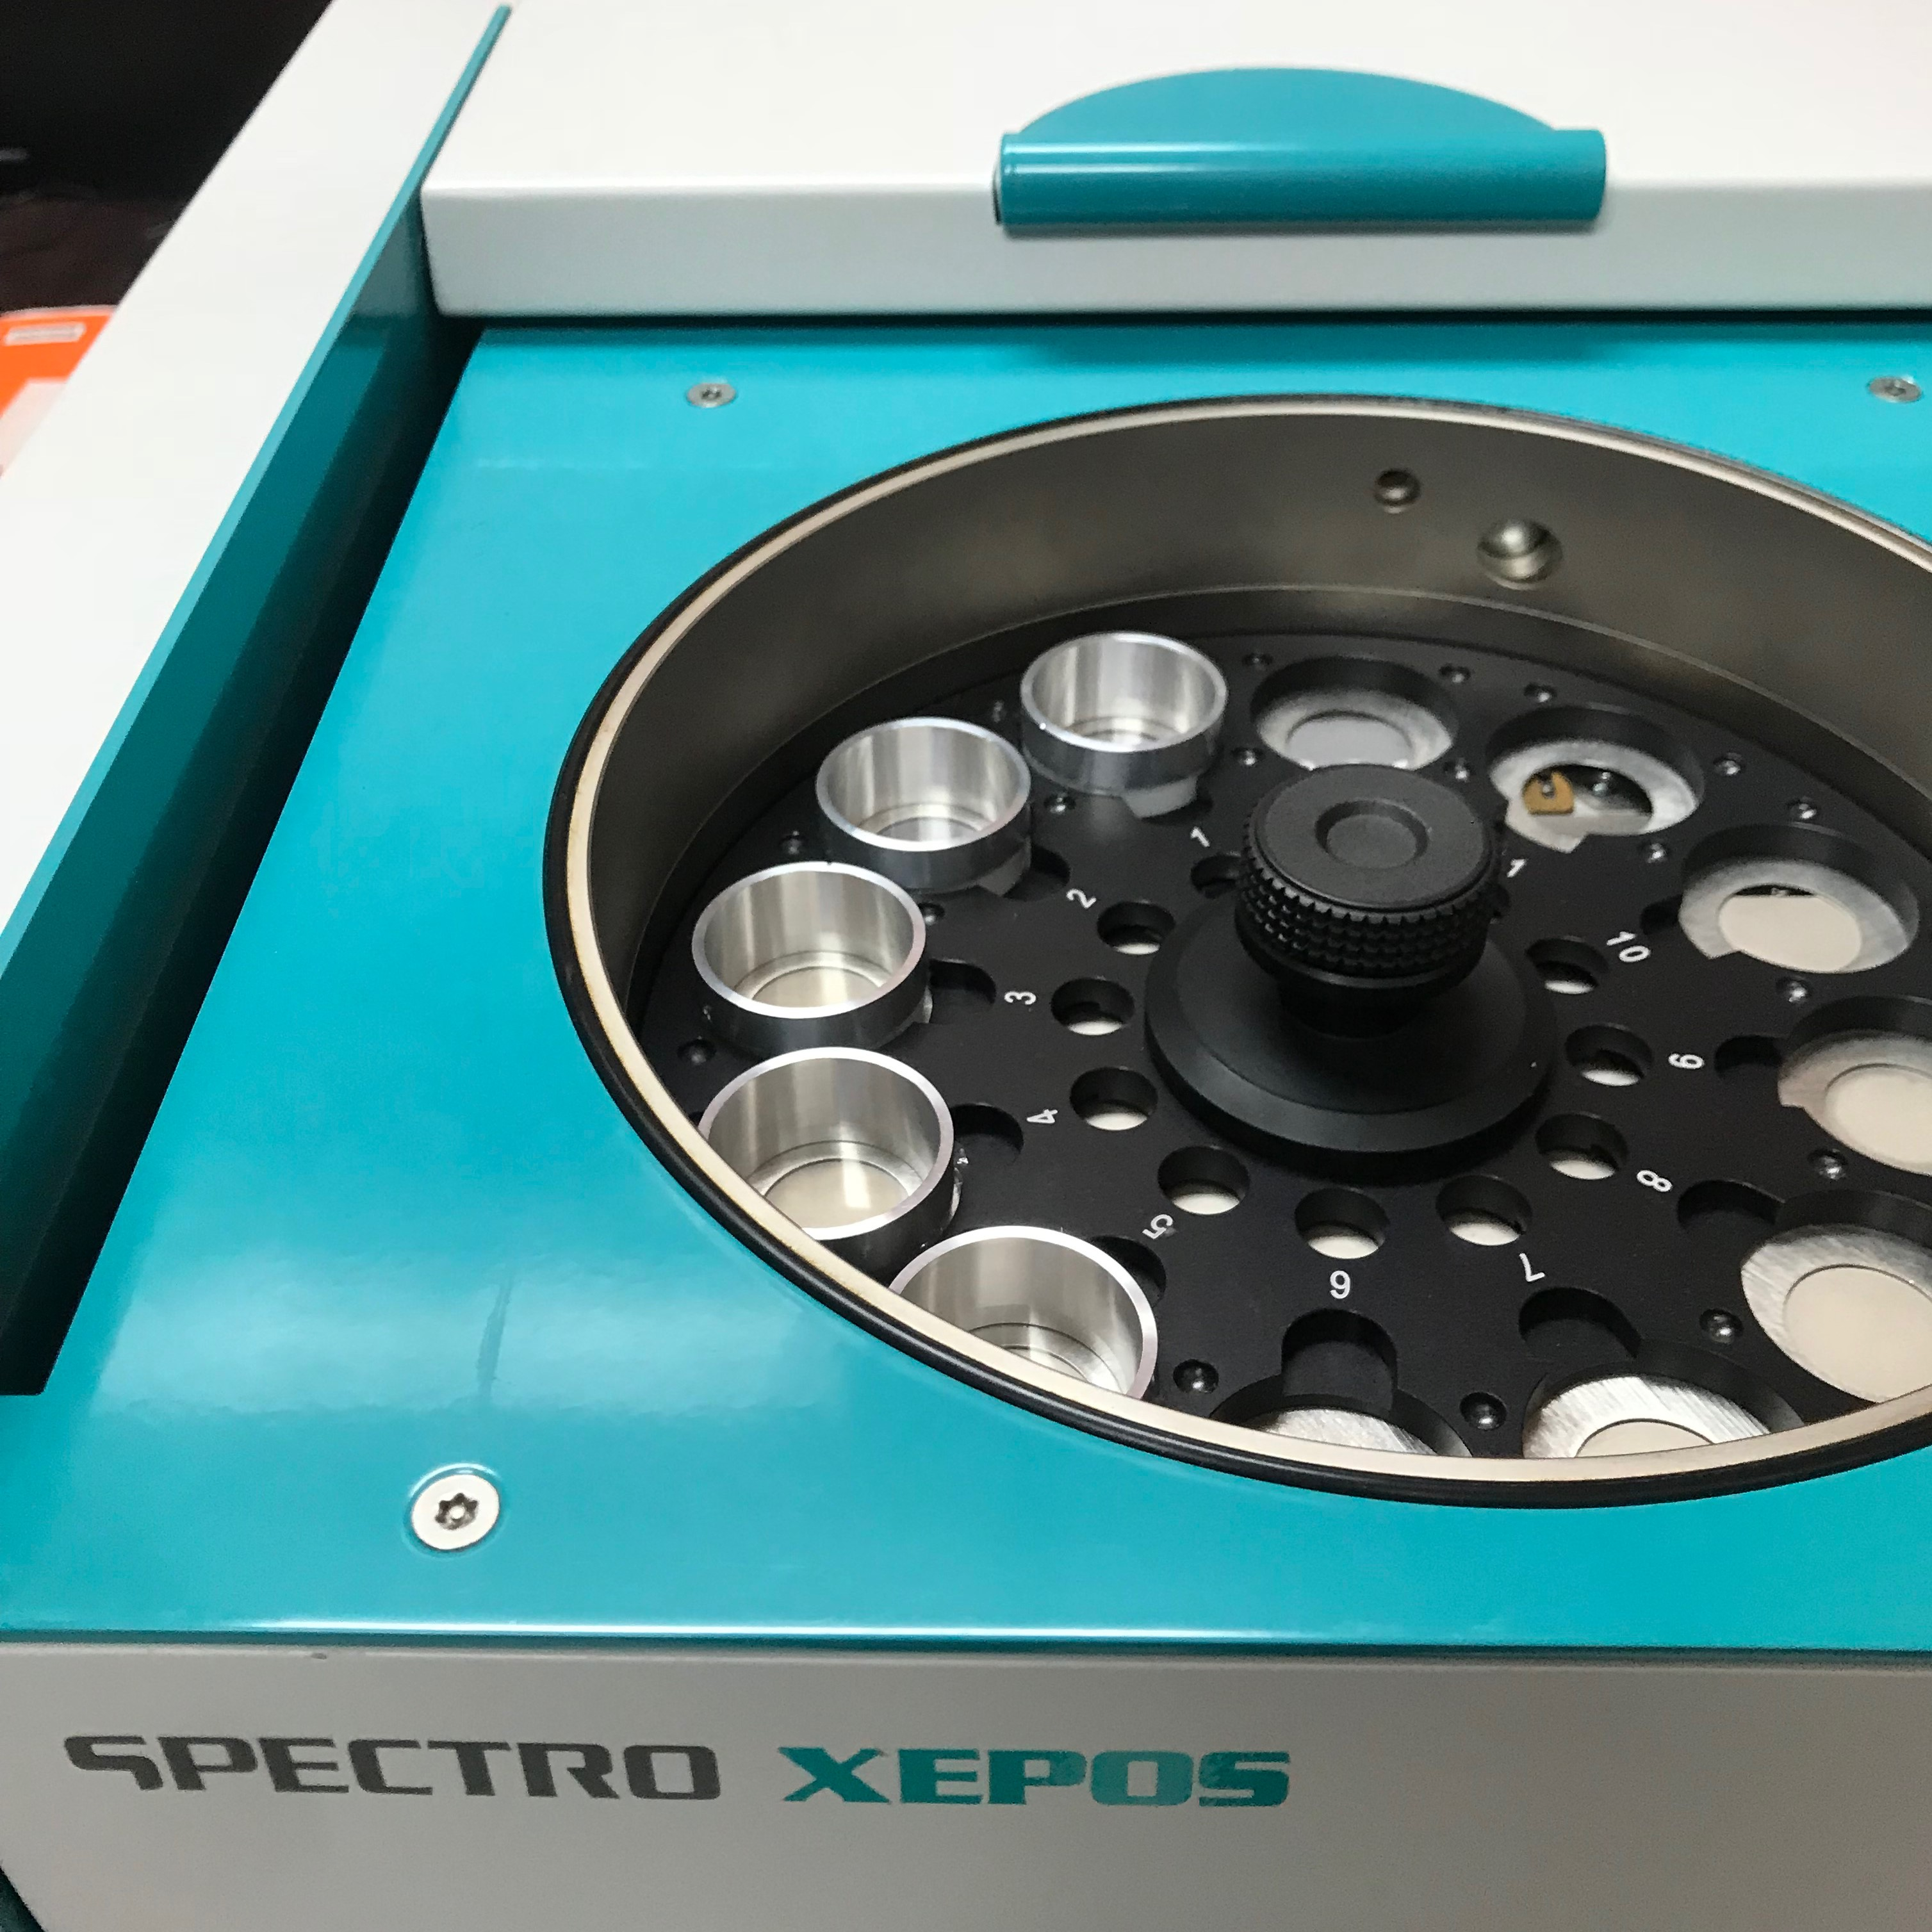
\includegraphics[width=0.35\textwidth]{Imagenes/XEPOS.jpg}
\caption{Vista superior equipo de fluorescencia de rayos X, \textit{SPECTRO XEPOS III}, del LGIG.}\label{Fig-XEPOS}
\end{figure}
	\section{Analizador elemental de carbono y nitrógeno}\label{Secc-CN}
La medida de la concentración de C y N se realizó mediante el analizador elemental por combustión (sección \ref{SubSec-CN-Intro}) \textit{Vario Micro Cube}, marca Elementar (Figura \ref{Fig-Elementar}). La cantidad de masa necesaria por muestra es de $\sim$ 20 mg. El porcentaje de carbono y nitrógeno se calcula a partir de una curva de calibración construida mediante Materiales de Referencia Certificados, y la incertidumbre en la medición se calcula a través de triplicados mediante una ecuación similar a la Ecuación \ref{Eq-SigmaRef}.
\begin{figure}[h]
\centering
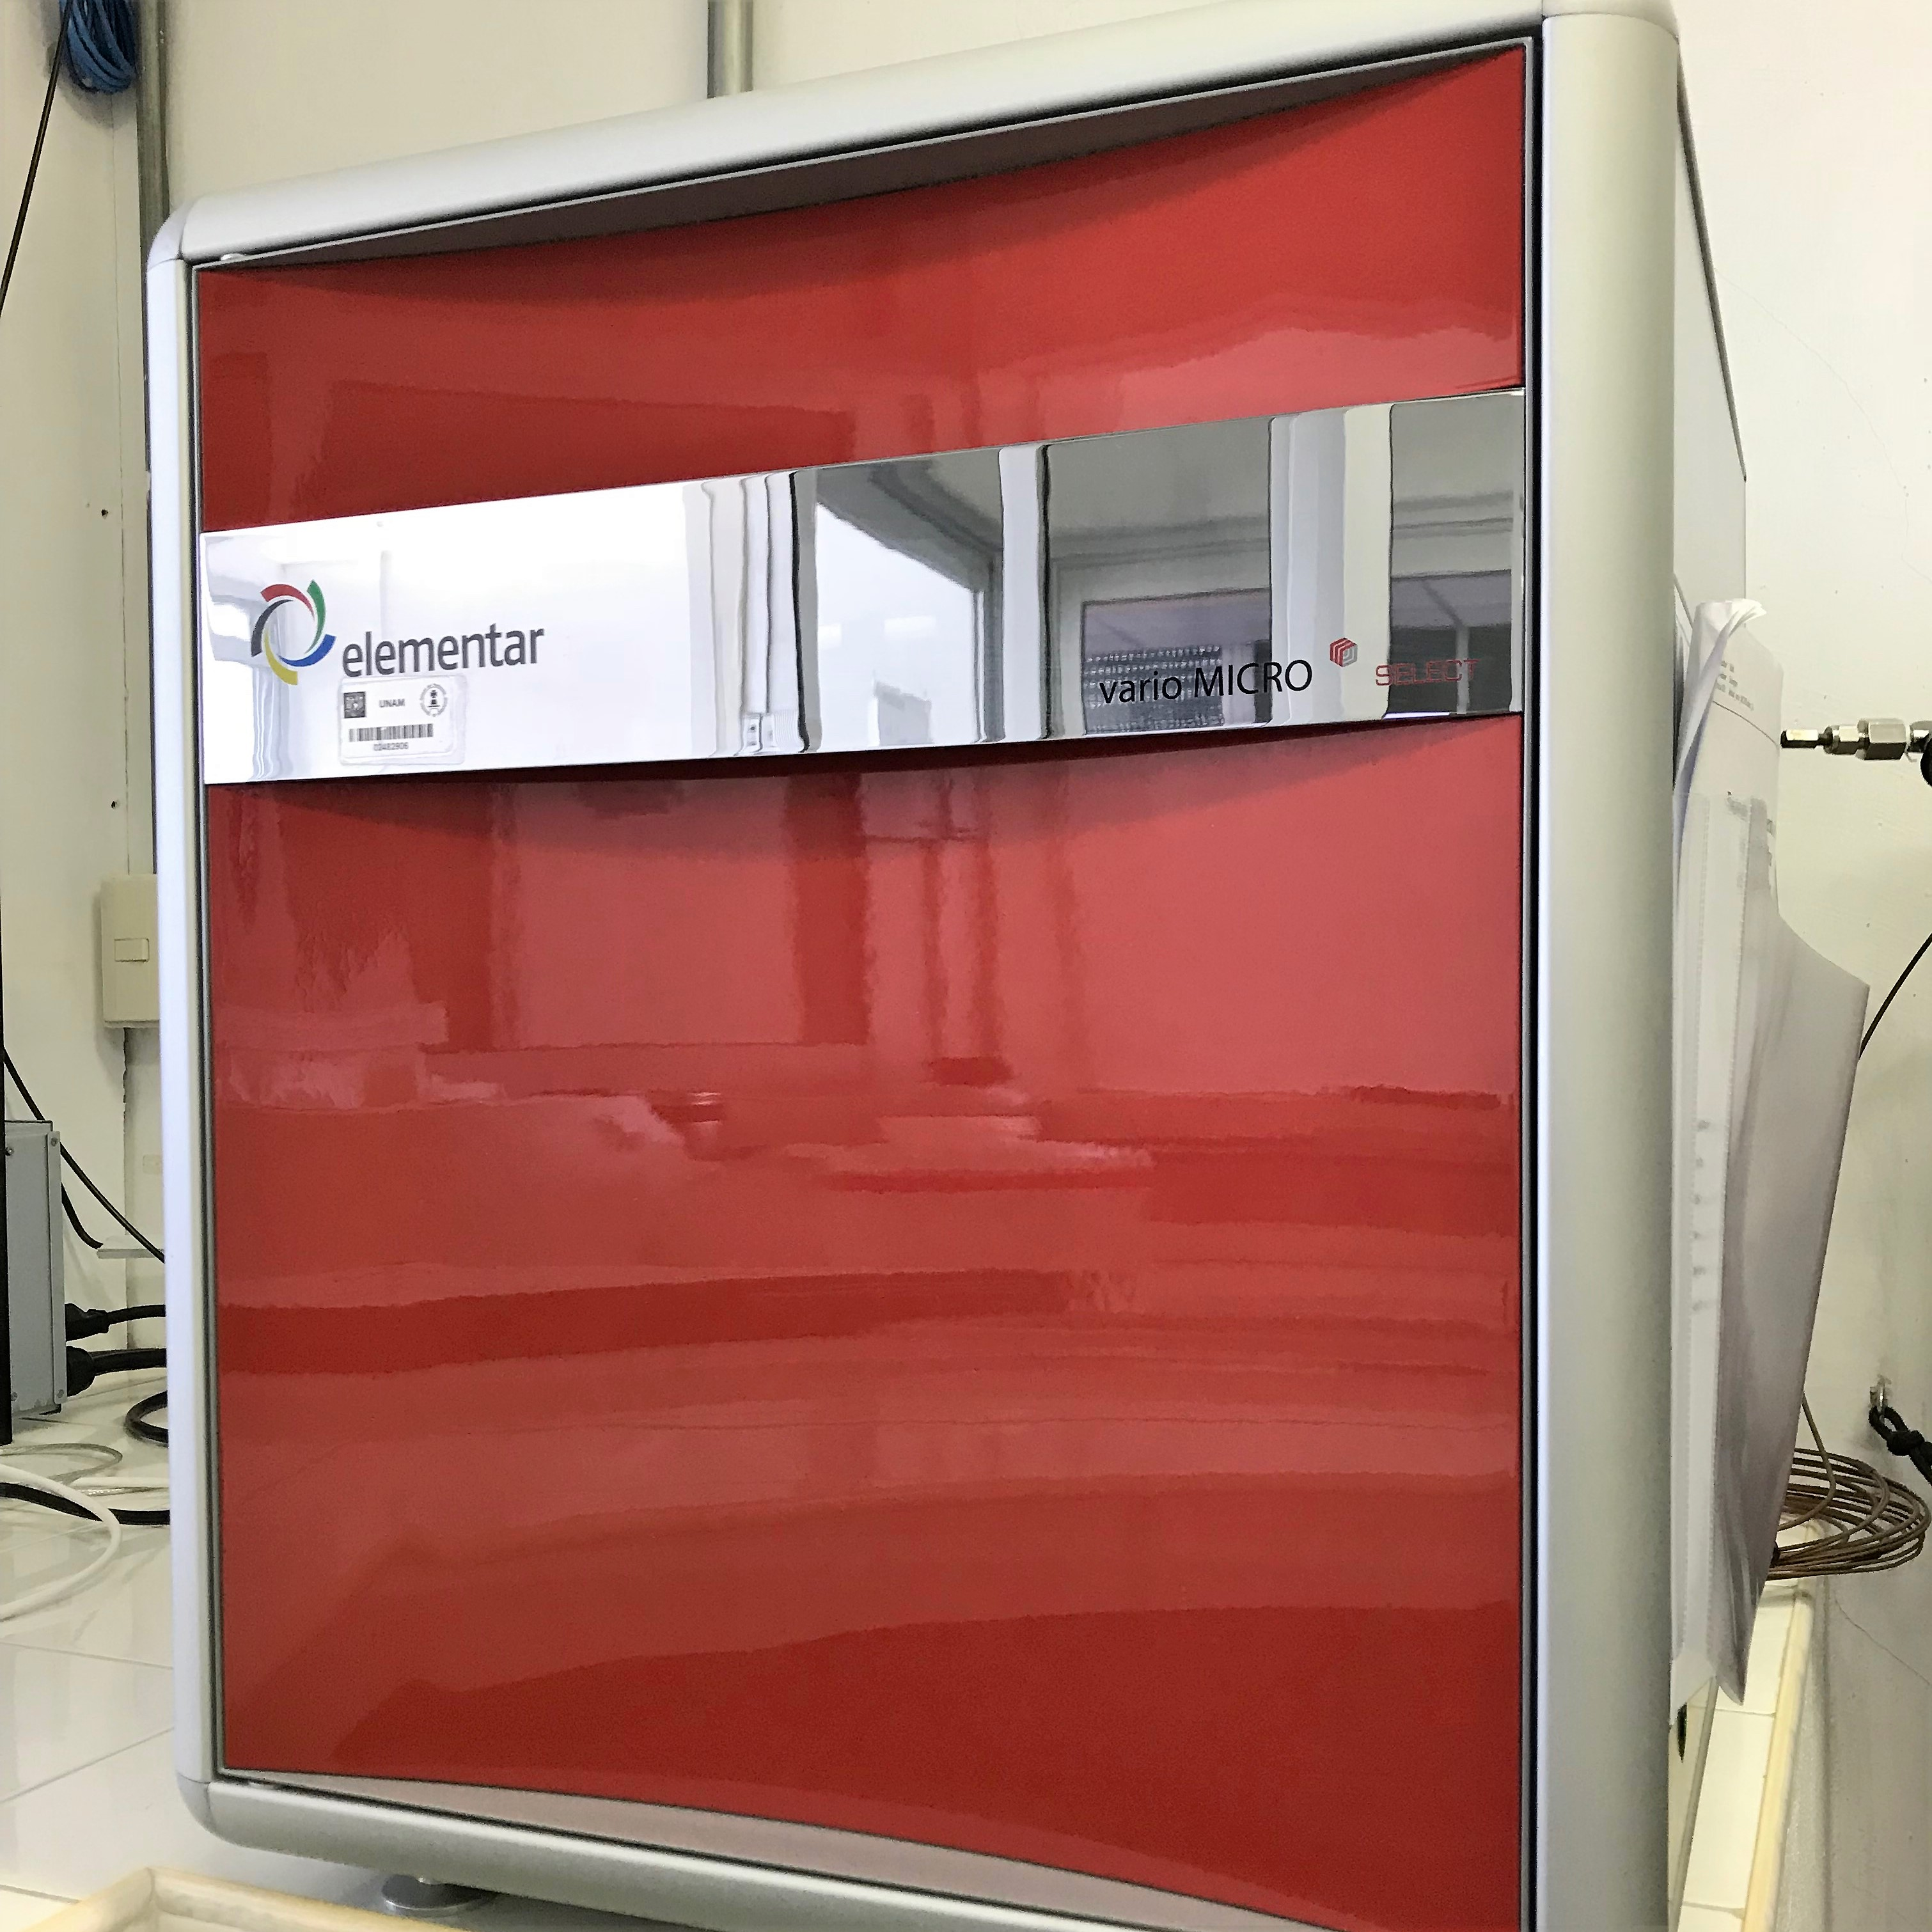
\includegraphics[width=0.35\textwidth]{Imagenes/Elementar.jpg}
\caption{Analizador elemental de carbono y nitrógeno \textit{Vario Micro Cube, Elementar}, empleado en el LGIG.}\label{Fig-Elementar}
\end{figure}
	\section[Definición de la composición elemental]{Definición de la composición elemental}\label{Secc-100Composicion}
Los elementos de la composición de cada sección de un núcleo sedimentario son conocidos excepto para algunos elementos, de los que podemos destacar H y O porque son constituyentes relevantes de la materia orgánica (fundamentalmente C, H y O) y de los carbonatos (Ca, C y O).
\\
\\
El porcentaje de C, N y en especial la relación C/N, se encuentran reportados para  algunos núcleos sedimentarios de zonas costeras, esteros, manglares y lagos, e.g. \cite{ramanathan2010management}, \cite{BARDHAN201590}, \cite{DUNN20082535}, \cite{TUE201887}. Sin embargo, el porcentaje de materia orgánica y su composición presentan una gran variabilidad entre ecosistemas, así como entre las muestras de un mismo núcleos sedimentario, por lo que es necesario determinar estos parámetros para cada muestra.
\\
\\
Para la simulación de la autoabsorción con ANGLE, es necesario conocer el 100 \% de la composición elemental de la muestra. Para ello, se calculó la fracción de composición desconocida y se atribuyó a la misma a la suma de H y O. 
\\
\\
Por ejemplo, si $x_i$ denota la concentración absoluta del elemento $i$, $\bigtriangleup$ denota la incertidumbre asociada y $x_\text{desconocido}$ denota el valor de la composición desconocida, entonces 
\begin{eqnarray}
x_\text{desconocido} &=& 1 - \biggl( x_\text{C} + x_\text{N} +  x_\text{Na} + x_\text{Mg} + \cdots + x_\text{U} \biggr), \\
\bigtriangleup x_\text{desconocido} &=& \sqrt{ 
(\bigtriangleup x_\text{C})^2 +
(\bigtriangleup x_\text{N})^2 +
(\bigtriangleup x_\text{Na})^2 +
(\bigtriangleup x_\text{Mg})^2 +
\cdots +
(\bigtriangleup x_\text{U})^2 }.
\end{eqnarray}
Si se establece que el porcentaje de contribución de oxígeno a la composición desconocida sea del 75 \%, la concentración de O e H y sus incertidumbres son 
\begin{eqnarray}
x_\text{O} = 0.75\times x_\text{desconocido}, & \hspace{1cm} & \bigtriangleup x_\text{O} = 0.75\times \bigtriangleup x_\text{desconocido}, \\
x_\text{H} = 0.25\times x_\text{desconocido}, & \hspace{1cm} & \bigtriangleup x_\text{H} = 0.25\times \bigtriangleup x_\text{desconocido}.
\end{eqnarray}
Así, existen dos composiciones: 
\begin{itemize}
\item composición de referencia (agua) y 
\item composición corregida establecida mediante el procedimento descrito anteriormente. 
\end{itemize}
Las cantidades que se relacionan con las composiciones son la eficiencia $\epsilon$, la actividad específica $A$ de un radionúclido y los resultados del fechado. La actividad corregida $A_\text{corr}$ se relaciona con la eficiencia corregida $\epsilon_{\text{corr}}$, la eficiencia de referencia $\epsilon_\text{ref}$ y la actividad de referencia $A_\text{ref}$ mediante
\begin{equation}\label{Eq-ActividadCorregida}
A_\text{corr} = \dfrac{\epsilon_\text{ref}}{\epsilon_{\text{corr}}}\,A_\text{ref}.
\end{equation}
	\section{Zonas de estudio}\label{Secc-ZonasSeleccionadas}
Las composiciones elementales de cada núcleo sedimentario dependen de un gran número de variables, tales como el tipo de ecosistema, el entorno geológico, la distancia a la costa, entre otros. Para el presente trabajo se seleccionaron núcleos sedimentarios pertenecientes a ecosistemas contrastantes (lagos, manglares, zona costera y mar abierto) de zonas diversas de México (ambiente terrígeno, Océano Pacífico, Golfo de México y Mar Caribe). Estos se encuentran consignados en la Tabla \ref{Table-ZonasSeleccionadas} y Figura \ref{Fig-Mapa}. 
\begin{table}[h]
\centering
\caption{Información de los núcleos sedimentarios analizados, incluyendo código, nombre extenso, zona geográfica de recolección y Gran Ecosistema Marino (LME) al que pertenece.}\label{Table-ZonasSeleccionadas}
\begin{tabular}{|c|c|c|c|}
	\hline								
\rowcolor{Blue2}	Código 	&	Nombre extenso	&	Zona geográfica	& 	LME	 \\	\hline
\rowcolor{Blue1}	GOMRI-500	&	Golfo de Mexico 500	&	Golfo de México	&	5	 \\	
\rowcolor{Blue1}	EU-VIII	&	Estero de Urias VIII	&	Sinaloa, Mazatlán	&	4	 \\	
\rowcolor{Blue1}	PCm	&	Punta Caracol manglar	&	Punta Caracol, Quintana Roo	&	12	 \\	
\rowcolor{Blue1}	LTAF	&	Laguna de Términos, Atasta Franja	&	El Carmén, Campeche	&	5	 \\	
\rowcolor{Blue1}	SAMO-14-2	&	Santa María del Oro 14-2	&	Santa María del Oro, Nayarit	&	NA 	 \\	
\rowcolor{Blue1}	TEHUA-XII	&	Tehuantepec  XII	&	Golfo de Tehuantepec	&	11	 \\	\hline
\end{tabular}
\end{table}
\begin{figure}[h]
\centering
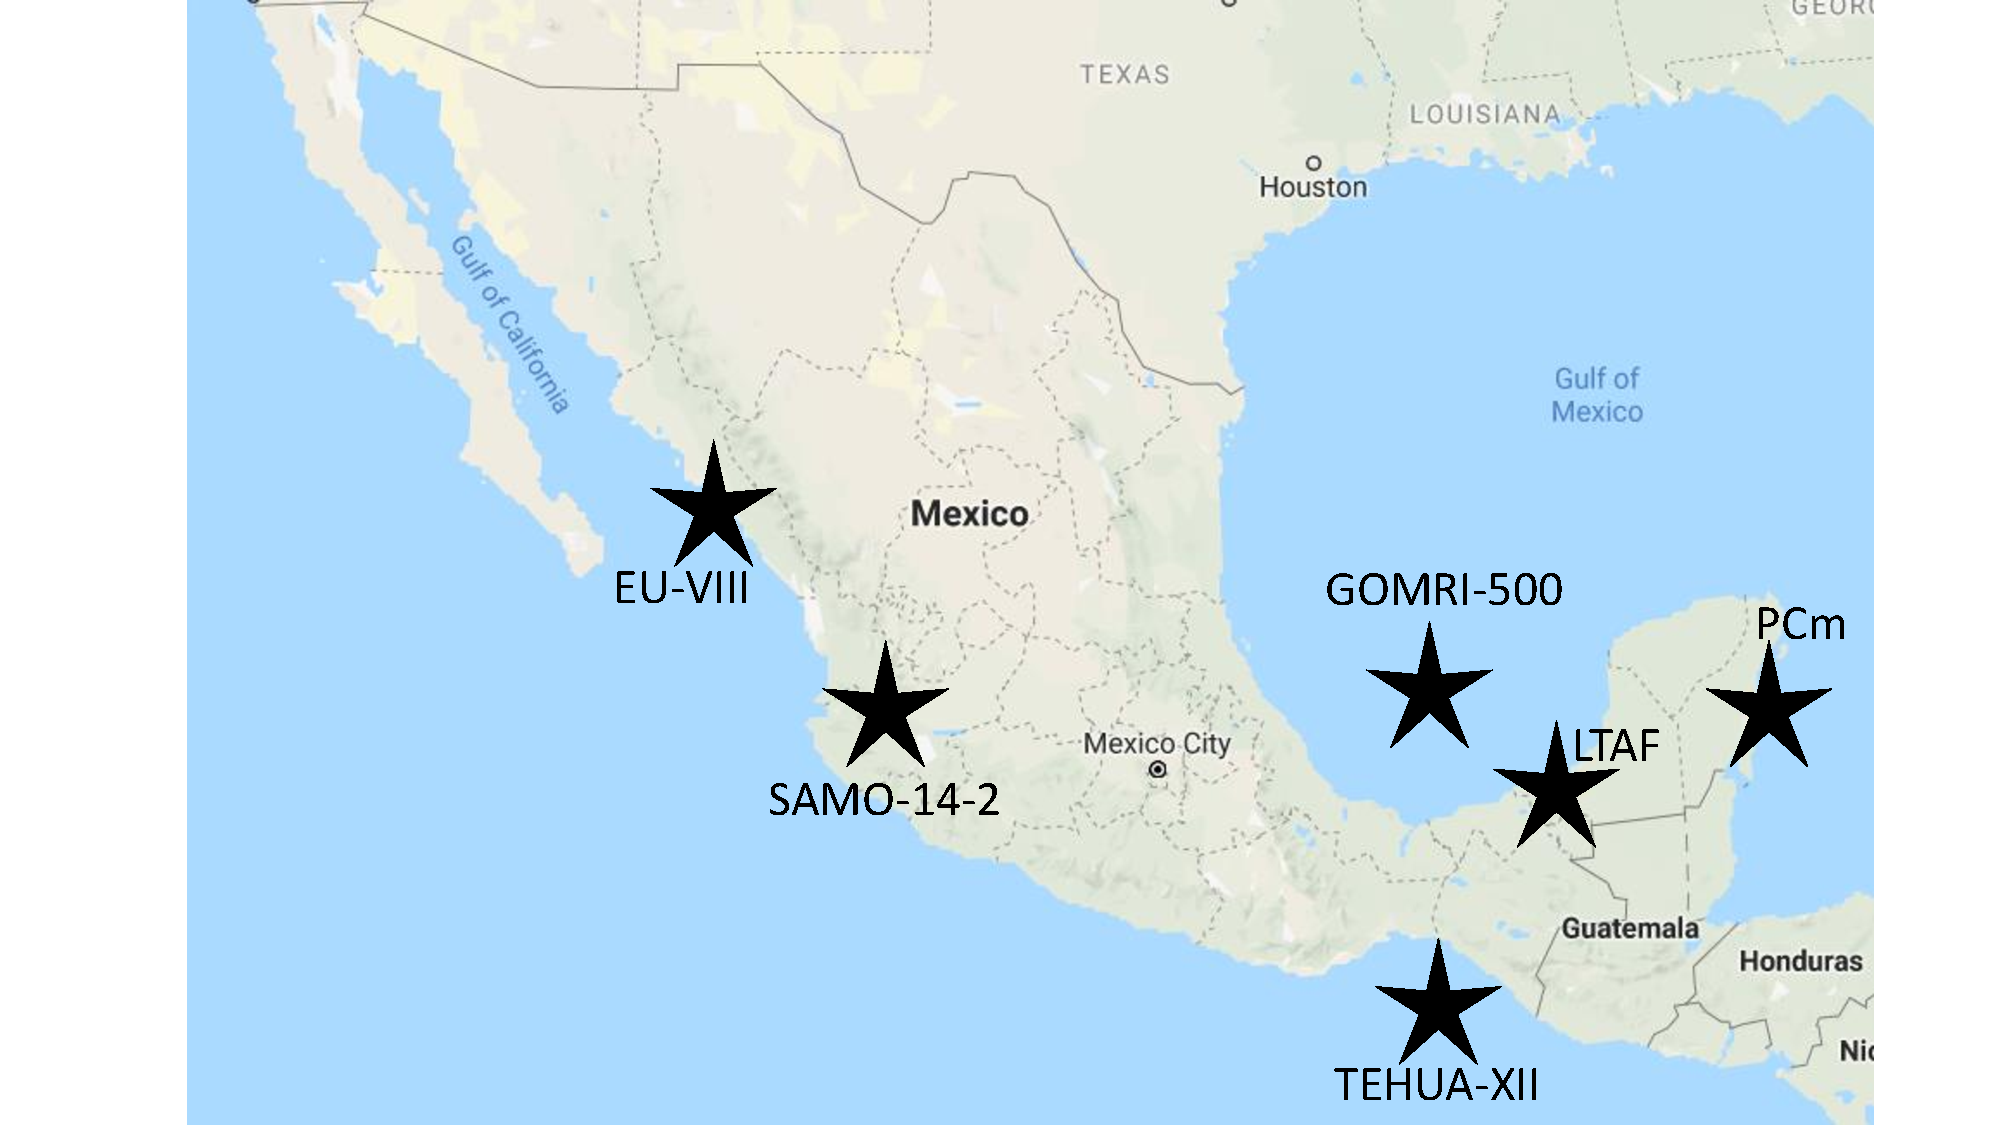
\includegraphics[width=\textwidth]{Imagenes/Mapa_Nucleos_Seleccionados.pdf}
\caption{Ubicación geográfica de los núcleos sedimentarios seleccionados para el presente trabajo.}\label{Fig-Mapa}
\end{figure}
\section[Códigos desarrollados]{Códigos desarrollados}\label{Secc-Codigos}
\subsection{Tratamiento de datos}
Los datos experimentales medidos de una sección de un núcleo sedimentario incluyen la actividad de los radionúclidos \PbCero\, y \PbCuatro\, obtenidos mediante espectrometría de rayos gamma y la composición elemental (Sección \ref{Secc-EspectrometriaGamma}) determinada por espectrometría de fluorescencia de rayos X (Sección \ref{Secc-EspectrometriaXRF}) y análisis elemental C-N (Sección \ref{Secc-CN}). Se generó un código en el lenguaje de programación R para leer, limpiar e integrar la información disponible para cada núcleo sedimentario, incluyendo la estimación del 100 \% de la composición elemental de cada sección (Sección \ref{Secc-100Composicion}) y el cálculo de la eficiencia corregida $\epsilon_\text{corr}$ para el sistema detector - muestra.
\\
\\
El código contempla los siguientes pasos: 1) limpiar los archivos originales, 2) definir 100 \% de la composición, 3) generar un archivo con la información relacionada con el tipo de detector, contenedor, composición, energías de interés, parámetros de ANGLE, 4) ejecutar ANGLE, y 5) leer los resultados de ANGLE.
\subsubsection{Manipulación de archivos originales}
La limpieza de los archivos generados por cualquier equipo se debe realizar debido a la posibilidad de resultados repetidos, errores de captura, entre otras. Esto debe ser realizado de forma automática para minimizar la manipulación manual de los resultados. En este trabajo se utilizaron resultados del analizador elemental C-N, XRF y espectrometría de rayos gamma.
\\
\\
La manipulación del archivo original de C-N se centra en la identificación de las filas a analizar y en el cálculo de las incertidumbres a través de los triplicados realizados. La identificación de las filas a analizar es necesario porque en un mismo archivo se almacenan los resultados de muestras de diversos núcleos. 
\\
\\
Para los resultados XRF, el código se enfoca en identificar las filas a analizar, eliminar valores negativos o valores reportados como menor o igual que el límite de detección, y convertir las concentraciones reportadas en porcentaje o partes por millón a concentraciones absolutas. Por ejemplo, una concentración de 5 \% de sodio significa una concentración absoluta de 0,05 de sodio. 
\\
\\
Los resultados de la espectrometría de rayos gamma son complejos pues albergan una gran cantidad de información. La finalidad del código es extraer información de cada archivo, correspondiente a una sección medida. La información extraída es la actividad, su incertidumbre y el límite de detección de los radionúclidos de interés, la fecha de medida, el detector y la geometría utilizada, el archivo de calibración, el método de análisis, el archivo de fondo utilizado, la masa y la densidad. 
\subsubsection{Definición de la composición de cada sección}
El procedimiento se describe en la Sección \ref{Secc-100Composicion}.
\subsubsection{Generación de archivo para ejecutar ANGLE}
La ejecución de ANGLE implica generar un archivo.SAVX que contiene toda la información requerida para su ejecución: detector (G1, G2, G3 o G4), vial (2 mL o 4 mL),  material (composición corregida) y curva de referencia.  Además, es necesario generar un archivo de bash (.sh) que contiene la instrucción de ejecutar ANGLE desde R. 
\subsubsection{Lectura de los resultados de ANGLE}
ANGLE genera archivos (.OUTX) que contienen el ángulo sólido efectivo y la eficiencia para las energías seleccionadas (Sección \ref{SubSec-ANGLE}). Esta eficiencia corregida $\epsilon_\text{corr}$, que tiene en cuenta el 100 \% de la composición y la densidad de la muestra, junto con la eficiencia de referencia $\epsilon_\text{ref}$ y la actividad de referencia extraída de los archivos .rpt $A_\text{ref}$, permite corregir la actividad $A_\text{corr}$ mediante la Ecuación \ref{Eq-ActividadCorregida}.
\subsection[Incertidumbre de eficiencia corregida ]{Incertidumbre de la eficiencia corregida}\label{SubSec-IncertidumbreEffMonteCarlo}
Se estimó que la mayor fuente de incertidumbre en la eficiencia corregida es la incertidumbre de la composición de la muestra (ver Apéndice \ref{SecResulIncertidumbreEffMonteCarlo}). Para calcularla, se realizó una simulación Monte Carlo variando la composición de cada elemento según una distribución normal, a partir de la concentración medida y su incertidumbre. Se hizo el mismo ejercicio con la densidad de la muestra. Esta simulación se realizó con una composición corregida de 50 \% oxígeno - 50 \% hidrógeno para una sección escogida al azar. La incertidumbre de la eficiencia corregida se calculó como la desviación estándar de los resultados generados mediante la simulación para cada una de las composiciones. 

\chapter{Resultados y discusión}
\lettrine{E}{}n la Sección \ref{Secc-ResultadosComposici} se muestran los resultados del análisis elemental de los seis núcleos sedimentarios de los  elementos mayoritarios: C, N, Na, Mg, Al, Si, S, Cl, K, Ca y Fe. El estudio de la fracción de la composición conocida indicó que en la mayoría de los núcleos sedimentarios se desconoce aproximadamente la mitad de la composición, salvo el núcleo sedimentario tipo manglar PCm en que se conoce el 74 \% de la composición. 
\\
\\
En la Sección \ref{Secc-EstimacionComposicion} se discute y se estandariza el porcentaje de oxígeno e hidrógeno para definir la composición corregida de cada sección de los núcleos sedimentarios. En la Sección \ref{Seccion-Correccion} se corrigen los perfiles de \PbCero\, debido a la composición y en la Sección \ref{Seccion-210y214} se discuten los perfiles corregidos de \PbCero, \PbCuatro\, y el equilibrio secular. 
\\
\\
El fechado mediante el modelo de Flujo Constante de los núcleos sedimentarios se describe en la Sección \ref{Seccion-Fechado} para los núcleos sedimentarios con una composición de referencia y una composición corregida, con un énfasis en la variabilidad de la eficiencia corregida y de las masas a lo largo del núcleo. 
	\section{Composición elemental de los núcleos sedimentarios}\label{Secc-ResultadosComposici}
Los resultados de la concentración a lo largo del núcleo de los ocho elementos de mayor concentración y la densidad promedio $\rho$ para los núcleos sedimentarios se muestran en la Tabla \ref{Tabla-ConcentracionDensidad} y en los diagramas de cajas de las Figuras \ref{Fig-ConcentracionNucleos1} - \ref{Fig-ConcentracionNucleos2}. Los extremos del intervalo de los diagramas de cajas corresponden a los valores de mínimo o máximo concentración, los extremos de la caja corresponden a los valores del primer y tercer cuartil, mientras el valor intermedio corresponde al segundo cuartil o mediana de la concentración a lo largo del núcleo.
\newpage
Las Figuras \ref{Fig-ConcentracionNucleos1} y \ref{Fig-ConcentracionNucleos2} muestran que la concentración absoluta de los elementos  de mayor contribución varía inter- e intra-núcleos. En relación con la variabilidad inter-núcleos, excepto para PCm, el elemento dominante promedio es el Si. El Si, como el Al, es habitualmente un indicador de las fuentes terrígenas \cite{Zabel2004}. Por otra parte, debido a que la península del Yucatán es una plataforma caliza, el núcleo sedimentario PCm no cuenta con Si ni Al entre los ocho elementos mayoritarios, es el único núcleo que presenta una contribución relevante de N (2 \%) y es el núcleo que presenta mayor contribución de C, 43 \% en promedio. Excluyendo este núcleo, todos los demás presentan una contribución promedio de C entre 3 \% - 12 \%. 
\\
\\
Por otro lado, salvo el núcleo sedimentario del lago de Santa María del Oro (SAMO-14-2), todos presentan una concentración relevante de Na y Cl, indicadores de fuentes marinas \cite{ruiz2016accretion}. El porcentaje promedio de la composición elemental conocida de los núcleos sedimentarios es menor al 50 \%, excepto para PCm (75 \%) y TEHUA-XII (66 \%). 
\\
\\
La variación de la composición intra-núcleos se evidencia en la dispersión de $\sum C$. La desviación estándar del promedio de la suma de los ocho elementos dominantes a lo largo de los núcleo PCm, LTAF y TEHUA-XII  es superior al 1 \%  (2\%, 14 \% y 7 \%, respectivamente). Los núcleos sedimentarios EU-VIII, GOMRI-500 y SAMO-14-2 presentan una desviación estándar menor que 1 \%, lo que sugiere la posibilidad de asumir una composición común para todas las secciones de estos núcleos.
\\
\\
La densidad promedio a lo largo de los núcleos sedimentarios (Tabla \ref{Tabla-ConcentracionDensidad}) se encuentra en un intervalo de 0.59 y 1.11 g cm$^{-3}$ y puede presentar variaciones a lo largo del mismo entre 0.11 g cm$^{-3}$ para GOMRI-500 hasta 0.43 g cm$^{-3}$ para LTAF. 
\begin{table}
\centering
\caption{Concentración absoluta promedio e intervalo de los ocho elementos de mayor contribución para cada núcleo sedimentario. Adicionalmente se muestra la suma de las concentraciones absolutas promedio medidas $\sum C$, y valor promedio $\overline{\rho}$, intervalo y variación $\bigtriangleup \rho$ de la densidad (en g cm$^{-3}$) a lo largo de los núcleos sedimentarios.}\label{Tabla-ConcentracionDensidad}
\begin{tabular}{|c|c|c|c|c|c|c|}\hline
\rowcolor{Blue3}	Elemento	&	EU-VIII	&	GOMRI-500	&	PCm	&	LTAF	&	SAMO-14-2	&	TEHUA-XII	\\ 	\hline	\hline
\rowcolor{Blue1}	C	&	0.07	&	0.03	&	0.43	&	0.12	&	0.08	&	0.06	\\ 		
\rowcolor{Blue1}		&	0.06-0.09	&	0.03-0.04	&	0.41-0.44	&	0.01-0.43	&	0.04-0.10	&	0.06-0.07	\\ 	\hline	
\rowcolor{Blue1}	N	&		&		&	0.02	&		&		&		\\ 		
\rowcolor{Blue1}		&		&		&	0.02-0.03	&		&		&		\\ 	\hline	
\rowcolor{Blue1}	Na	&	0.08	&	0.02	&	0.11	&	0.02	&		&	0.13	\\ 		
\rowcolor{Blue1}		&	0.07-0.09	&	0.01-0.03	&	0.07-0.14	&	0.01-0.04	&		&	0.09-0.17	\\ 	\hline	
\rowcolor{Blue1}	Mg	&		&		&	0.02	&	0.01	&	0.01	&	0.03	\\ 		
\rowcolor{Blue1}		&		&		&	0.01-0.03	&	0.01-0.01	&	0.00-0.01	&	0.02-0.04	\\ 	\hline	
\rowcolor{Blue1}	Al	&	0.07	&	0.07	&		&	0.06	&	0.04	&	0.09	\\ 		
\rowcolor{Blue1}		&	0.07-0.08	&	0.07-0.08	&		&	0.03-0.07	&	0.02-0.08	&	0.06-0.11	\\ 	\hline	
\rowcolor{Blue1}	Si	&	0.17	&	0.20	&		&	0.20	&	0.19	&	0.24	\\ 		
\rowcolor{Blue1}		&	0.16-0.18	&	0.18-0.23	&		&	0.08-0.23	&	0.16-0.27	&	0.18-0.28	\\ 	\hline	
\rowcolor{Blue1}	S 	&	0.03	&		&	0.04	&		&	0.01	&		\\ 		
\rowcolor{Blue1}		&	0.01-0.04	&		&	0.02-0.06	&		&	0.00-0.01	&		\\ 	\hline	
\rowcolor{Blue1}	Cl	&	0.05	&	0.02	&	0.11	&		&		&	0.06	\\ 		
\rowcolor{Blue1}		&	0.04-0.06	&	0.01-0.02	&	0.08-0.14	&		&		&	0.05-0.08	\\ 	\hline	
\rowcolor{Blue1}	K	&	0.02	&	0.02	&	0.002	&	0.02	&	0.01	&		\\ 		
\rowcolor{Blue1}		&	0.02-0.02	&	0.02-0.02	&	0.002-0.004	&	0.01-0.02	&	0.00-0.02	&		\\ 	\hline	
\rowcolor{Blue1}	Ca	&		&	0.07	&	0.01	&	0.01	&	0.12	&	0.03	\\ 		
\rowcolor{Blue1}		&		&	0.06-0.07	&	0.00-0.04	&	0.01-0.02	&	0.06-0.18	&	0.02-0.04	\\ 	\hline	
\rowcolor{Blue1}	Fe	&	0.03	&	0.03	&		&	0.04	&	0.02	&	0.03	\\ 		
\rowcolor{Blue1}		&	0.03-0.04	&	0.03-0.04	&		&	0.02-0.06	&	0.00-0.04	&	0.03-0.03	\\ 	\hline	\hline
\rowcolor{Blue2}	$\sum C$	&	0.53	&	0.46	&	0.74	&	0.48	&	0.47	&	0.66	\\ 	\hline	\hline
\rowcolor{Blue2}	$\overline{\rho}$	&	1.04	&	1.11	&	0.59	&	1.07	&	0.84	&	0.81	\\ 
\rowcolor{Blue2}	Intervalo de $\rho$	&	0.99-1.15	&	1.06-1.17	&	0.52-0.74	&	0.75-1.18	&	0.71-0.98	&	0.61-0.86	\\ 	
\rowcolor{Blue2}	 $\bigtriangleup \rho$ & 0.16	&	0.11	&	0.22	&	0.43	&	0.27	&	0.25 \\ \hline
\end{tabular}
\end{table}
\begin{figure}
\centering
\includegraphics[width=0.9\textwidth]{Imagenes/XRF_Todos_Los_Nucleos_1.png}
\caption{Diagrama de cajas de los núcleos sedimentarios EU-VIII, GOMRI-500 y PCm para los ochos elementos de mayor concentración. Para cada núcleo sedimentario se incluye el valor porcentual de la suma promedio de las concentraciones medidas $\sum C$.}\label{Fig-ConcentracionNucleos1}
\end{figure}
\begin{figure}
\centering
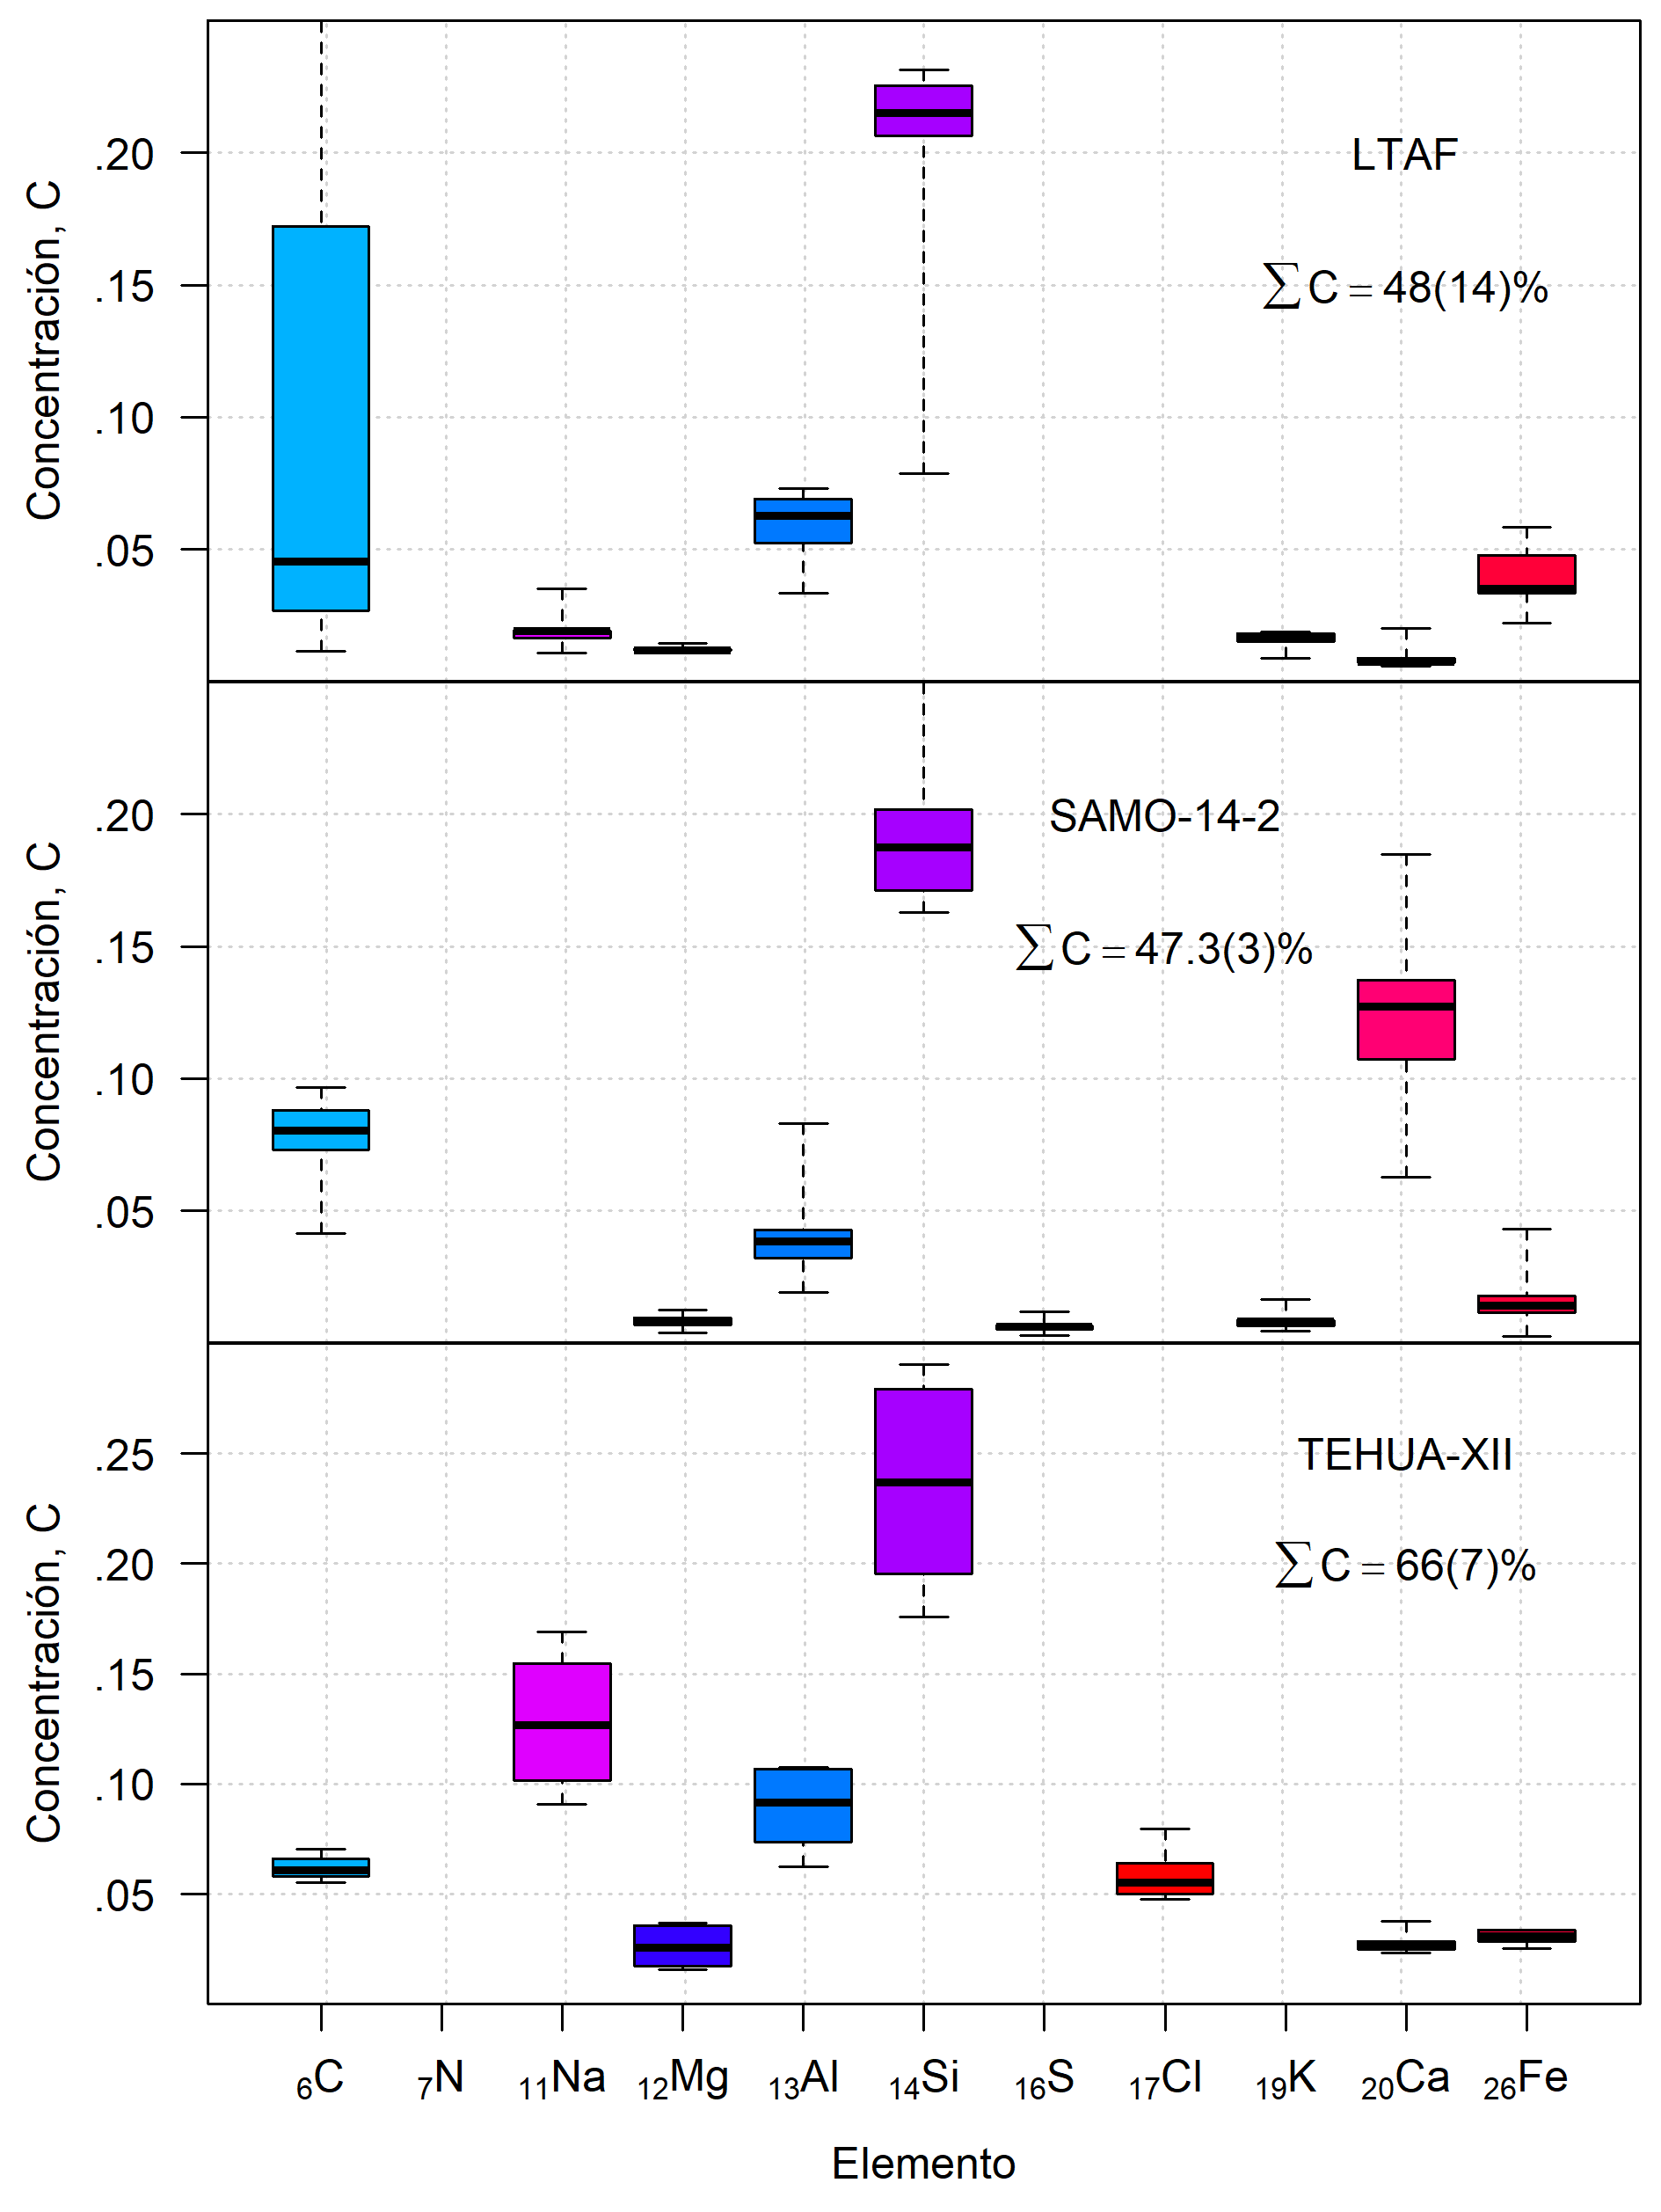
\includegraphics[width=0.9\textwidth]{Imagenes/XRF_Todos_Los_Nucleos_2.png}
\caption{Diagrama de cajas de los núcleos sedimentarios LTAF, SAMO-14-2 y TEHUA-XII para los ochos elementos de mayor concentración.  Para cada núcleo sedimentario se incluye el valor porcentual de la suma promedio de las concentraciones medidas $\sum C$.}\label{Fig-ConcentracionNucleos2}
\end{figure}
\newpage
	\section{Estimación de la composición desconocida}\label{Secc-EstimacionComposicion}
Una vez establecida la composición conocida, es necesario realizar una estimación de la composición desconocida de cada muestra. En la Tabla \ref{Tabla-Eficiencias} se muestran las diferencias porcentuales promedio de los valores de la eficiencia corregida para 46.54 keV respecto a la eficiencia de referencia para composiciones desconocidas de 0 \%, 50 \% y 100 \% de oxígeno. La variación porcentual promedio es del 3 \% para todos los núcleos sedimentarios analizados, y varía entre 0.8 \% y 4 \%. La incertidumbre típica de las actividades de \PbCero\, y \PbCuatro, medidas por espectrometría de rayos gamma, es típicamente mayor al 6 \%. Se consideró que el uso de una composición corregida con el 50 \% oxígeno en la fracción desconocida es aceptable porque la desviación promedio calculada (3 \%) es inferior a la incertidumbre de la medida.
\\
\\
Para los núcleos sedimentarios considerados, la corrección mínima realizada (1.7 \%, Tabla \ref{Tabla-Eficiencias}) fue para PCm. Efectivamente, el componente mayoritario de este núcleo es el átomo ligero C, con una atenuación por autoabsorción mínima, por lo que se podría asumir en este caso que la composición de referencia puede ser utilizada sin correcciones debido a la composición. Podemos concluir que para muestras con un alto contenido de materia orgánica, en general, no es necesario aplicar correcciones por autoabsorción.
\\ \\ 
En los otros casos, las diferencias promedio entre las eficiencias de referencia y corregida son relevantes, e ignorar su corrección puede inducir a errores substanciales en la cuantificación de las actividades de \PbCero\, en las muestras. En promedio, estos errores son aproximadamente del 10 \% para EU-VIII, LTAF, SAMO-14-2 y TEHUA-XII, y de 16 \% para GOMRI-500. Concluimos que la corrección por densidad y autoabsorción es necesaria cuando la determinación de la actividad absoluta de \PbCero\, es importante.
\begin{table}[h]
\centering
\caption{Diferencia porcentual promedio de las eficiencias para 46.54 keV respecto a la calibración de referencia para diferentes composiciones desconocidas de H y O.}\label{Tabla-Eficiencias}
\begin{tabular}{|c|c|c|c|c|}\hline
\rowcolor{Blue3}	Núcleo 	&	 \multicolumn{3}{c|}{Dif. porcentual promedio en $\epsilon$}           					&	Variación en Dif. 	\\ 	
\rowcolor{Blue3}	 sedimentario & \multicolumn{3}{c|}{$\overline{\epsilon} \pm \bigtriangleup \epsilon$}   & porcentuales \\	\hline
\rowcolor{Blue2}		&	0 \% Oxígeno 	&	\textbf{50 \% Oxígeno} 	&	100 \% Oxígeno 	&	0 \%  $\rightarrow$ 100 \% 	\\  \hline
\rowcolor{Blue1}	EU-VIII	&	$13 \pm 1$	&	$12 \pm 1$	&	$11 \pm 1$	&	2	\\ 	
\rowcolor{Blue1}	GOMRI-500	&	$18 \pm 1$	&	$16 \pm 1$	&	$14 \pm 1$	&	4	\\ 	
\rowcolor{Blue1}	PCm	&	$1.3 \pm 0.9$	&	$1.7 \pm 0.8$	&	$2.1 \pm 0.9$	&	0.8	\\ 	
\rowcolor{Blue1}	LTAF	&	$14 \pm 5$	&	$12 \pm 4$	&	$10 \pm 4$	&	4	\\ 	
\rowcolor{Blue1}	SAMO-14-2	&	$10 \pm 2$	&	$8.5 \pm 1.9$	&	$7 \pm 2$	&	3	\\ 	
\rowcolor{Blue1}	TEHUA-XIII	&	$9 \pm 1$	&	$8 \pm 2$	&	$7 \pm 2$	&	2	\\ 	\hline
\rowcolor{Blue2}	 & \multicolumn{3}{r|}{Promedio:} 							&	3	\\ 	\hline
\end{tabular}
\end{table}	
\newpage
	\section{Corrección de las actividades de \PbCero}\label{Seccion-Correccion}
Una vez se ha estimado la composición corregida de la muestra, se calcularon las eficiencias corregidas para cada una de las secciones medidas y se determinaron las actividades corregidas. Los perfiles de actividad específica de \PbCero, con una composición de referencia y corregida, y su diferencia porcentual, se presentan en las Figuras \ref{FigEUVIIIAgua}, \ref{FigGOMRI500Agua}, \ref{FigPCmAgua}, \ref{FigLTAFAgua}, \ref{FigSAMO142Agua} y \ref{FigTEHUAXIIAgua}. Los rangos de actividad específica y profundidad de los anterior perfiles varían entre núcleos sedimentarios.
\\
\\
En todos los casos, se confirmó la presencia de exceso porque todos los perfiles muestran un decrecimiento con la profundidad. En el caso de los núcleos EU-VIII, PCm y SAMO-14-2, las diferencias observadas entre los dos perfiles son pequeñas y los perfiles son similares, dentro de la banda de incertidumbre. 
\\
\\
Sin embargo, para los núcleos GOMRI-500 y TEHUA-XII (ambos de ambientes de mar abierto y con baja concentración de C) las diferencias de las actividades de \PbCero, debidas a las correcciones de composición y densidad, son significativas sobretodo en la parte superior del núcleo, que contiene la mayor parte del inventario de \PbCeroEx, por lo que \textit{a priori} es de esperar que sean los núcleos donde el fechado sea más afectado por estas correcciones.
\begin{figure}
\centering
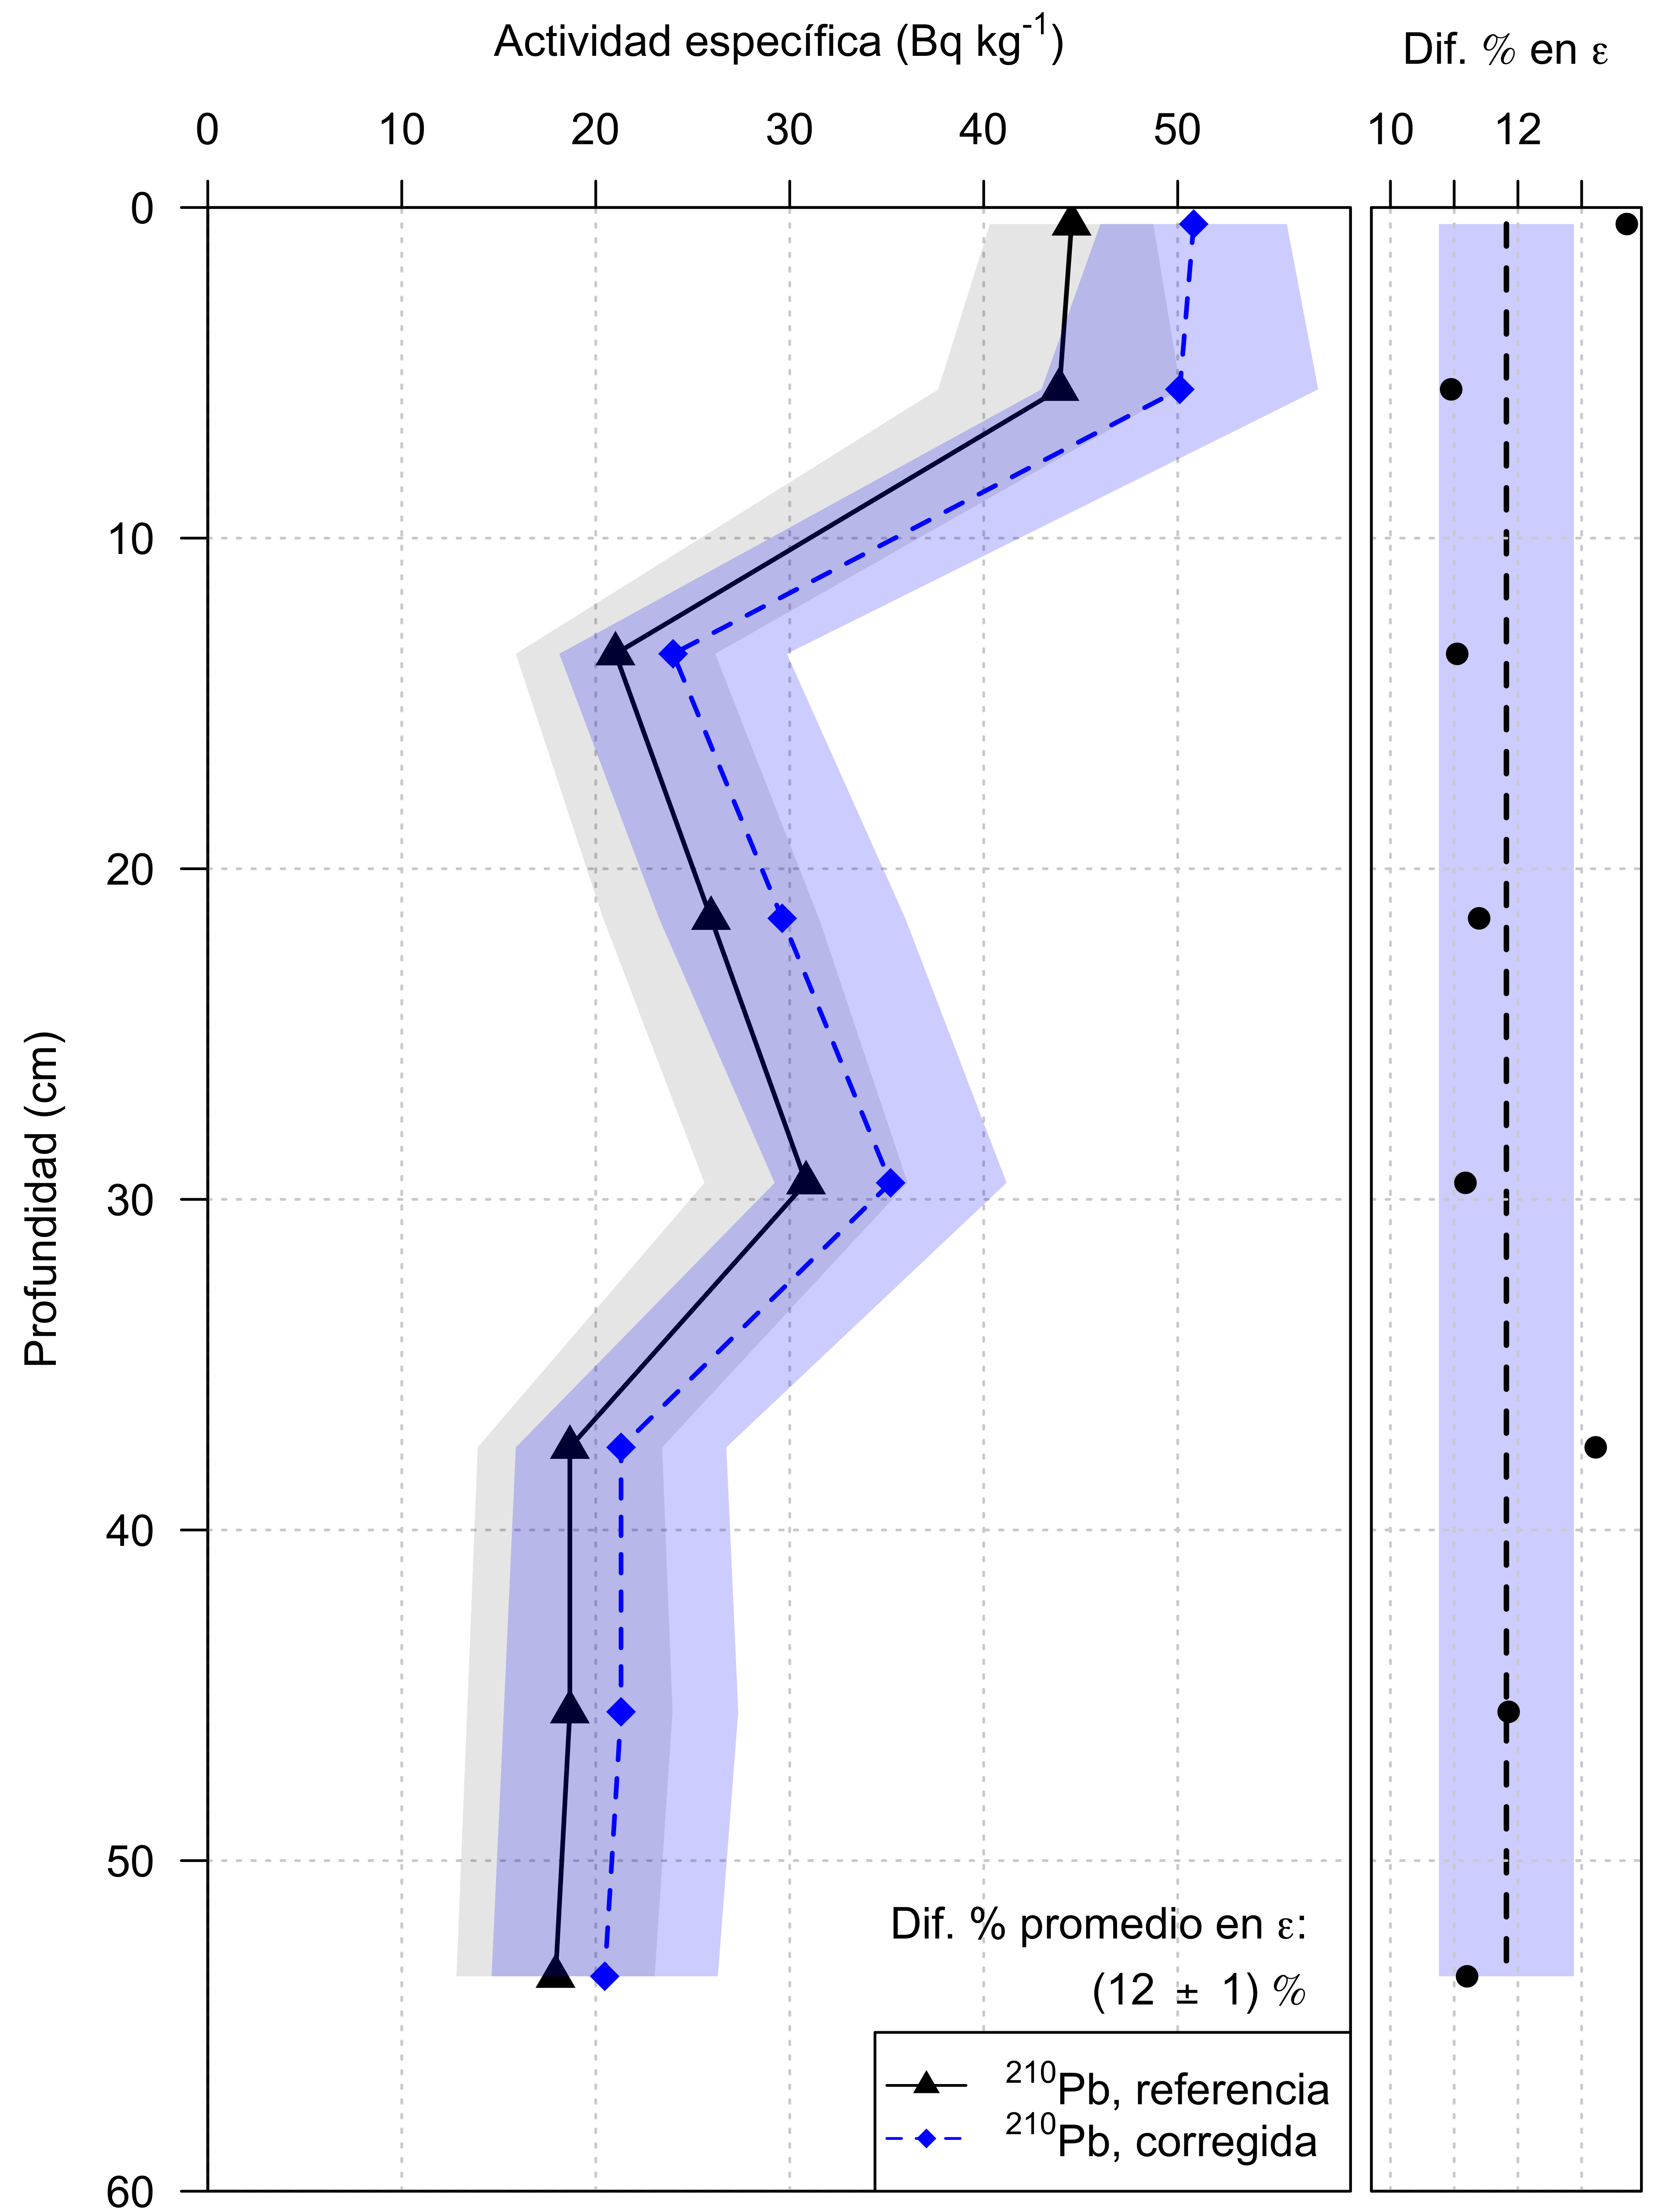
\includegraphics[width=0.9\textwidth]{Imagenes/Act_210Pb_Agua_Composicion_EU_VIII.png}
\caption{Perfil de actividad específica de \PbCero\, para el núcleo \textbf{EU-VIII} asumiendo una composición elemental de referencia y una composición corregida (Sección \ref{Secc-100Composicion}). Se muestra la diferencia porcentual promedio en el valor las eficiencias de referencia y corregida para una energía de 46.54 keV.}\label{FigEUVIIIAgua}
\end{figure}
\begin{figure}
\centering
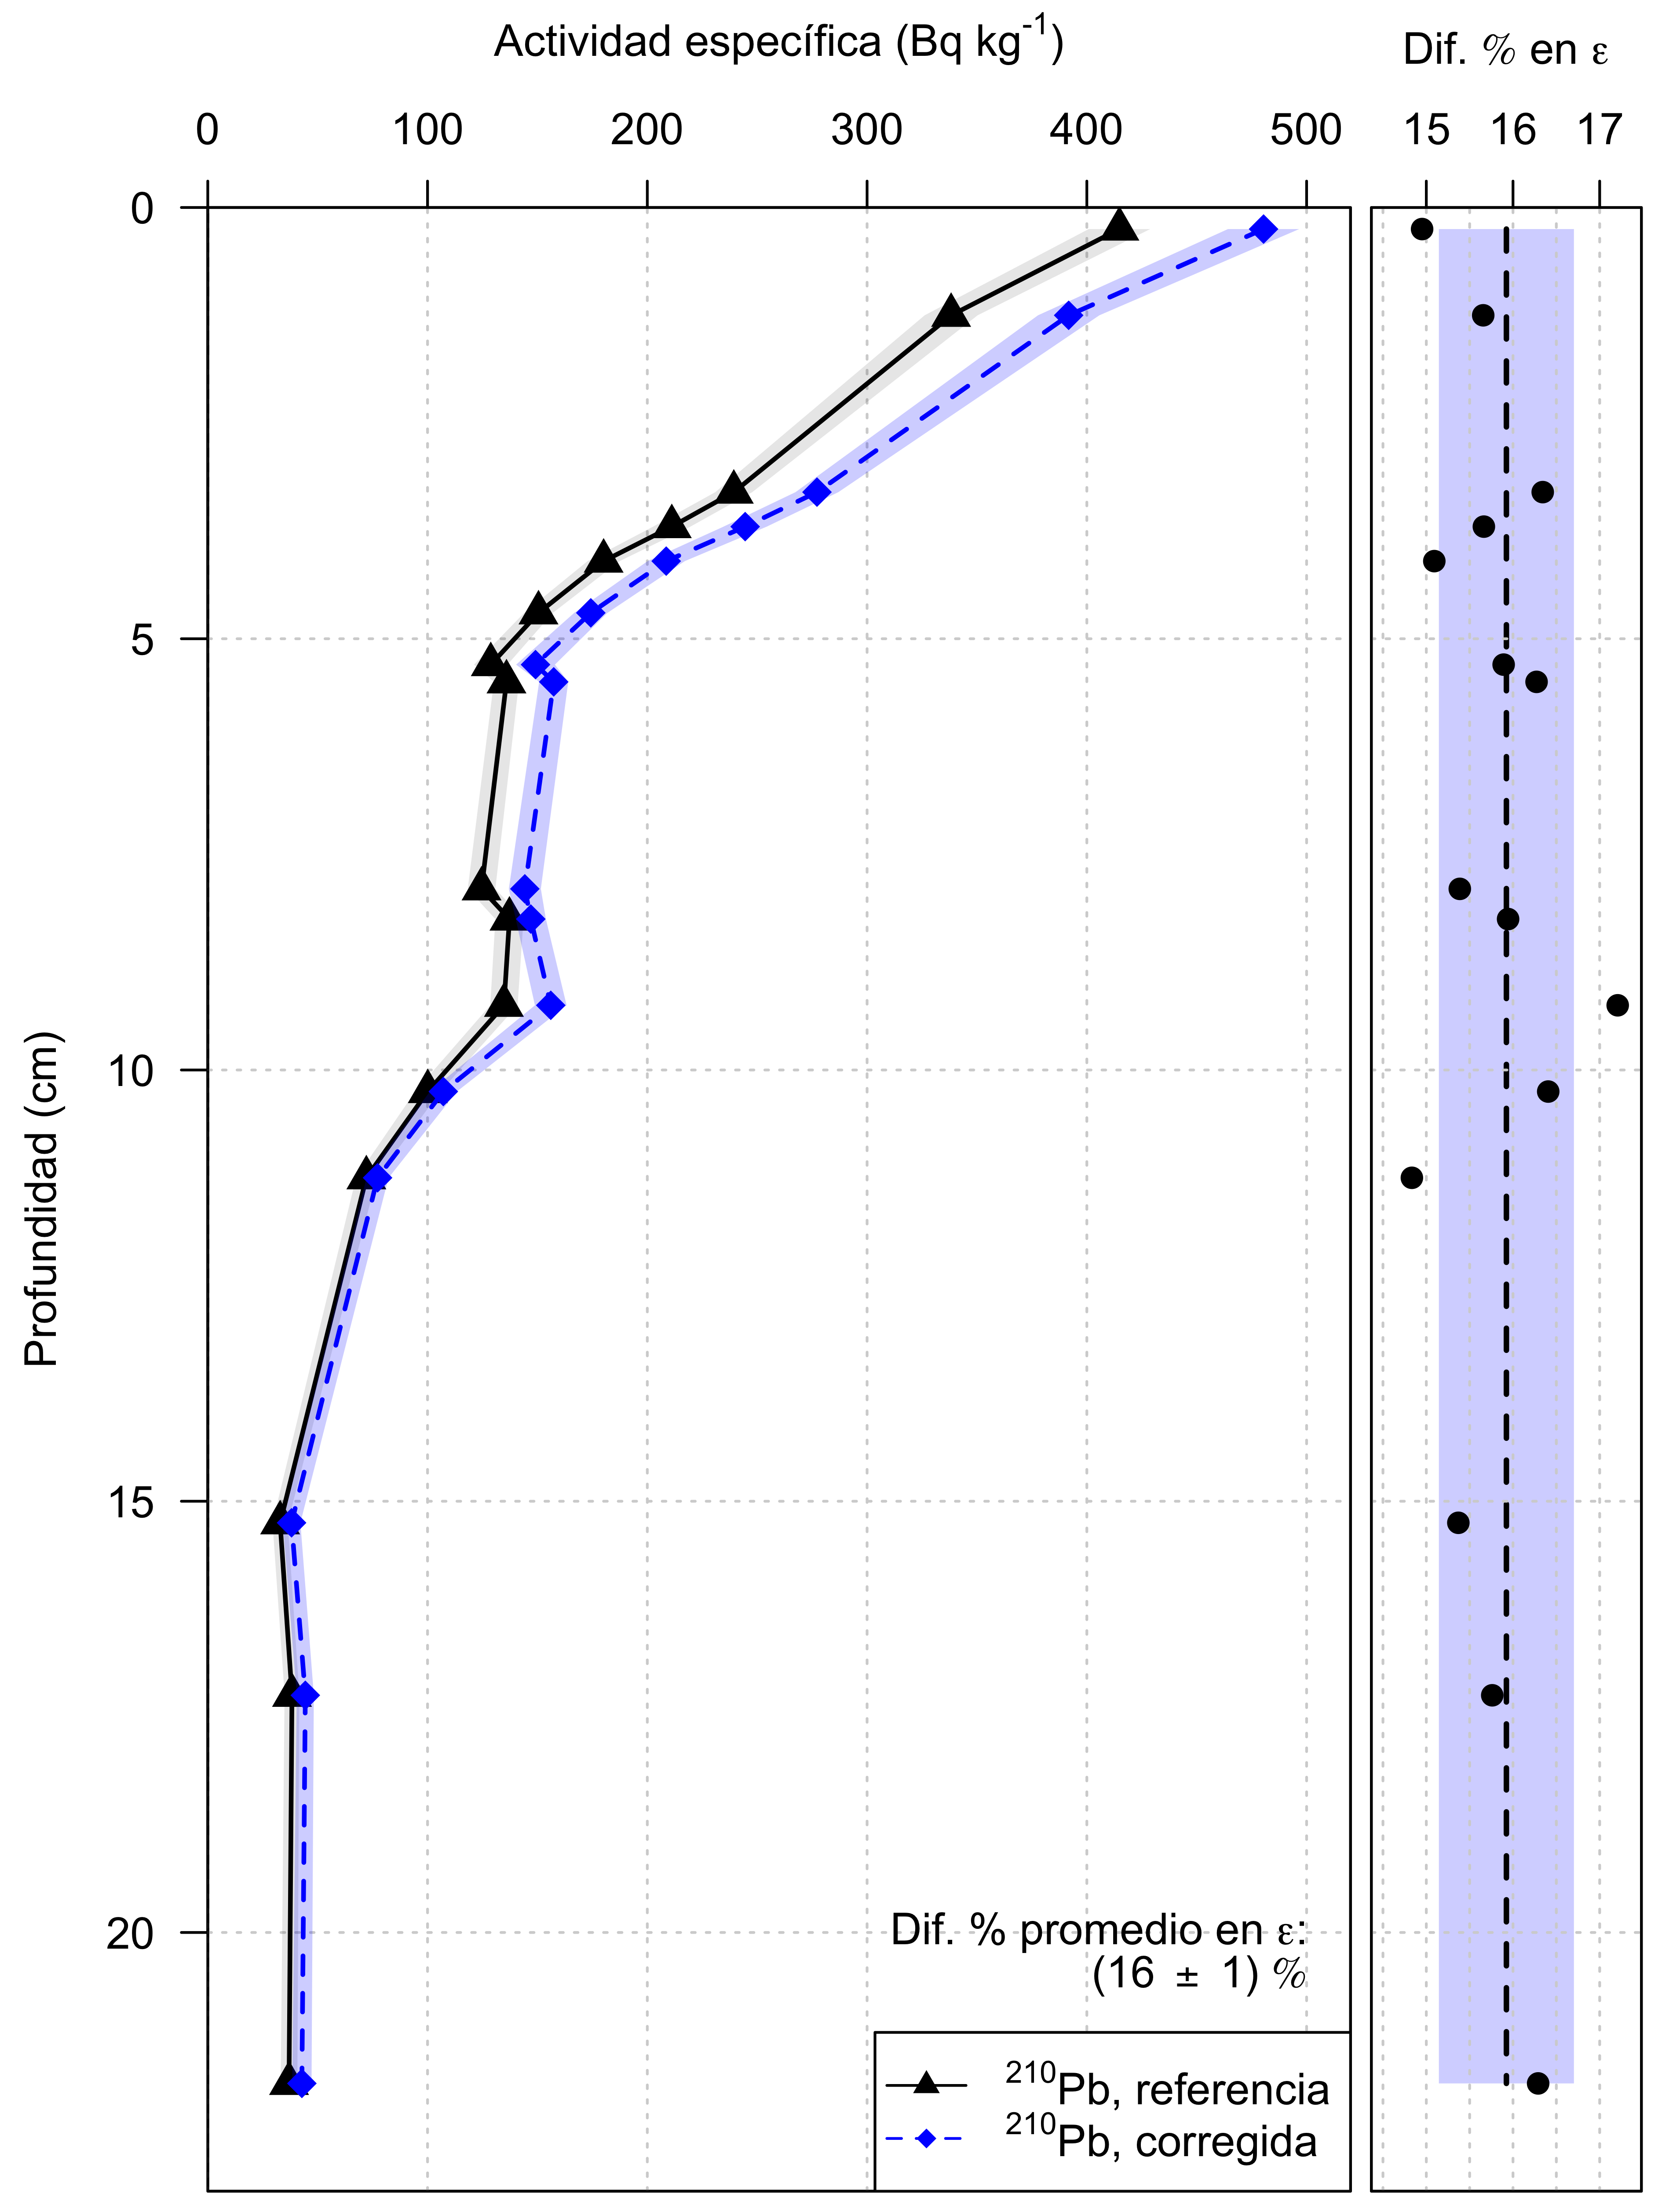
\includegraphics[width=0.9\textwidth]{Imagenes/Act_210Pb_Agua_Composicion_GOMRI_500.png}
\caption{Perfil de actividad específica de \PbCero\, para el núcleo \textbf{GOMRI-500} asumiendo una composición elemental de referencia y una composición corregida (Sección \ref{Secc-100Composicion}). Se muestra la diferencia porcentual promedio en el valor las eficiencias de referencia y corregida para una energía de 46.54 keV.}\label{FigGOMRI500Agua}
\end{figure}
\begin{figure}
\centering
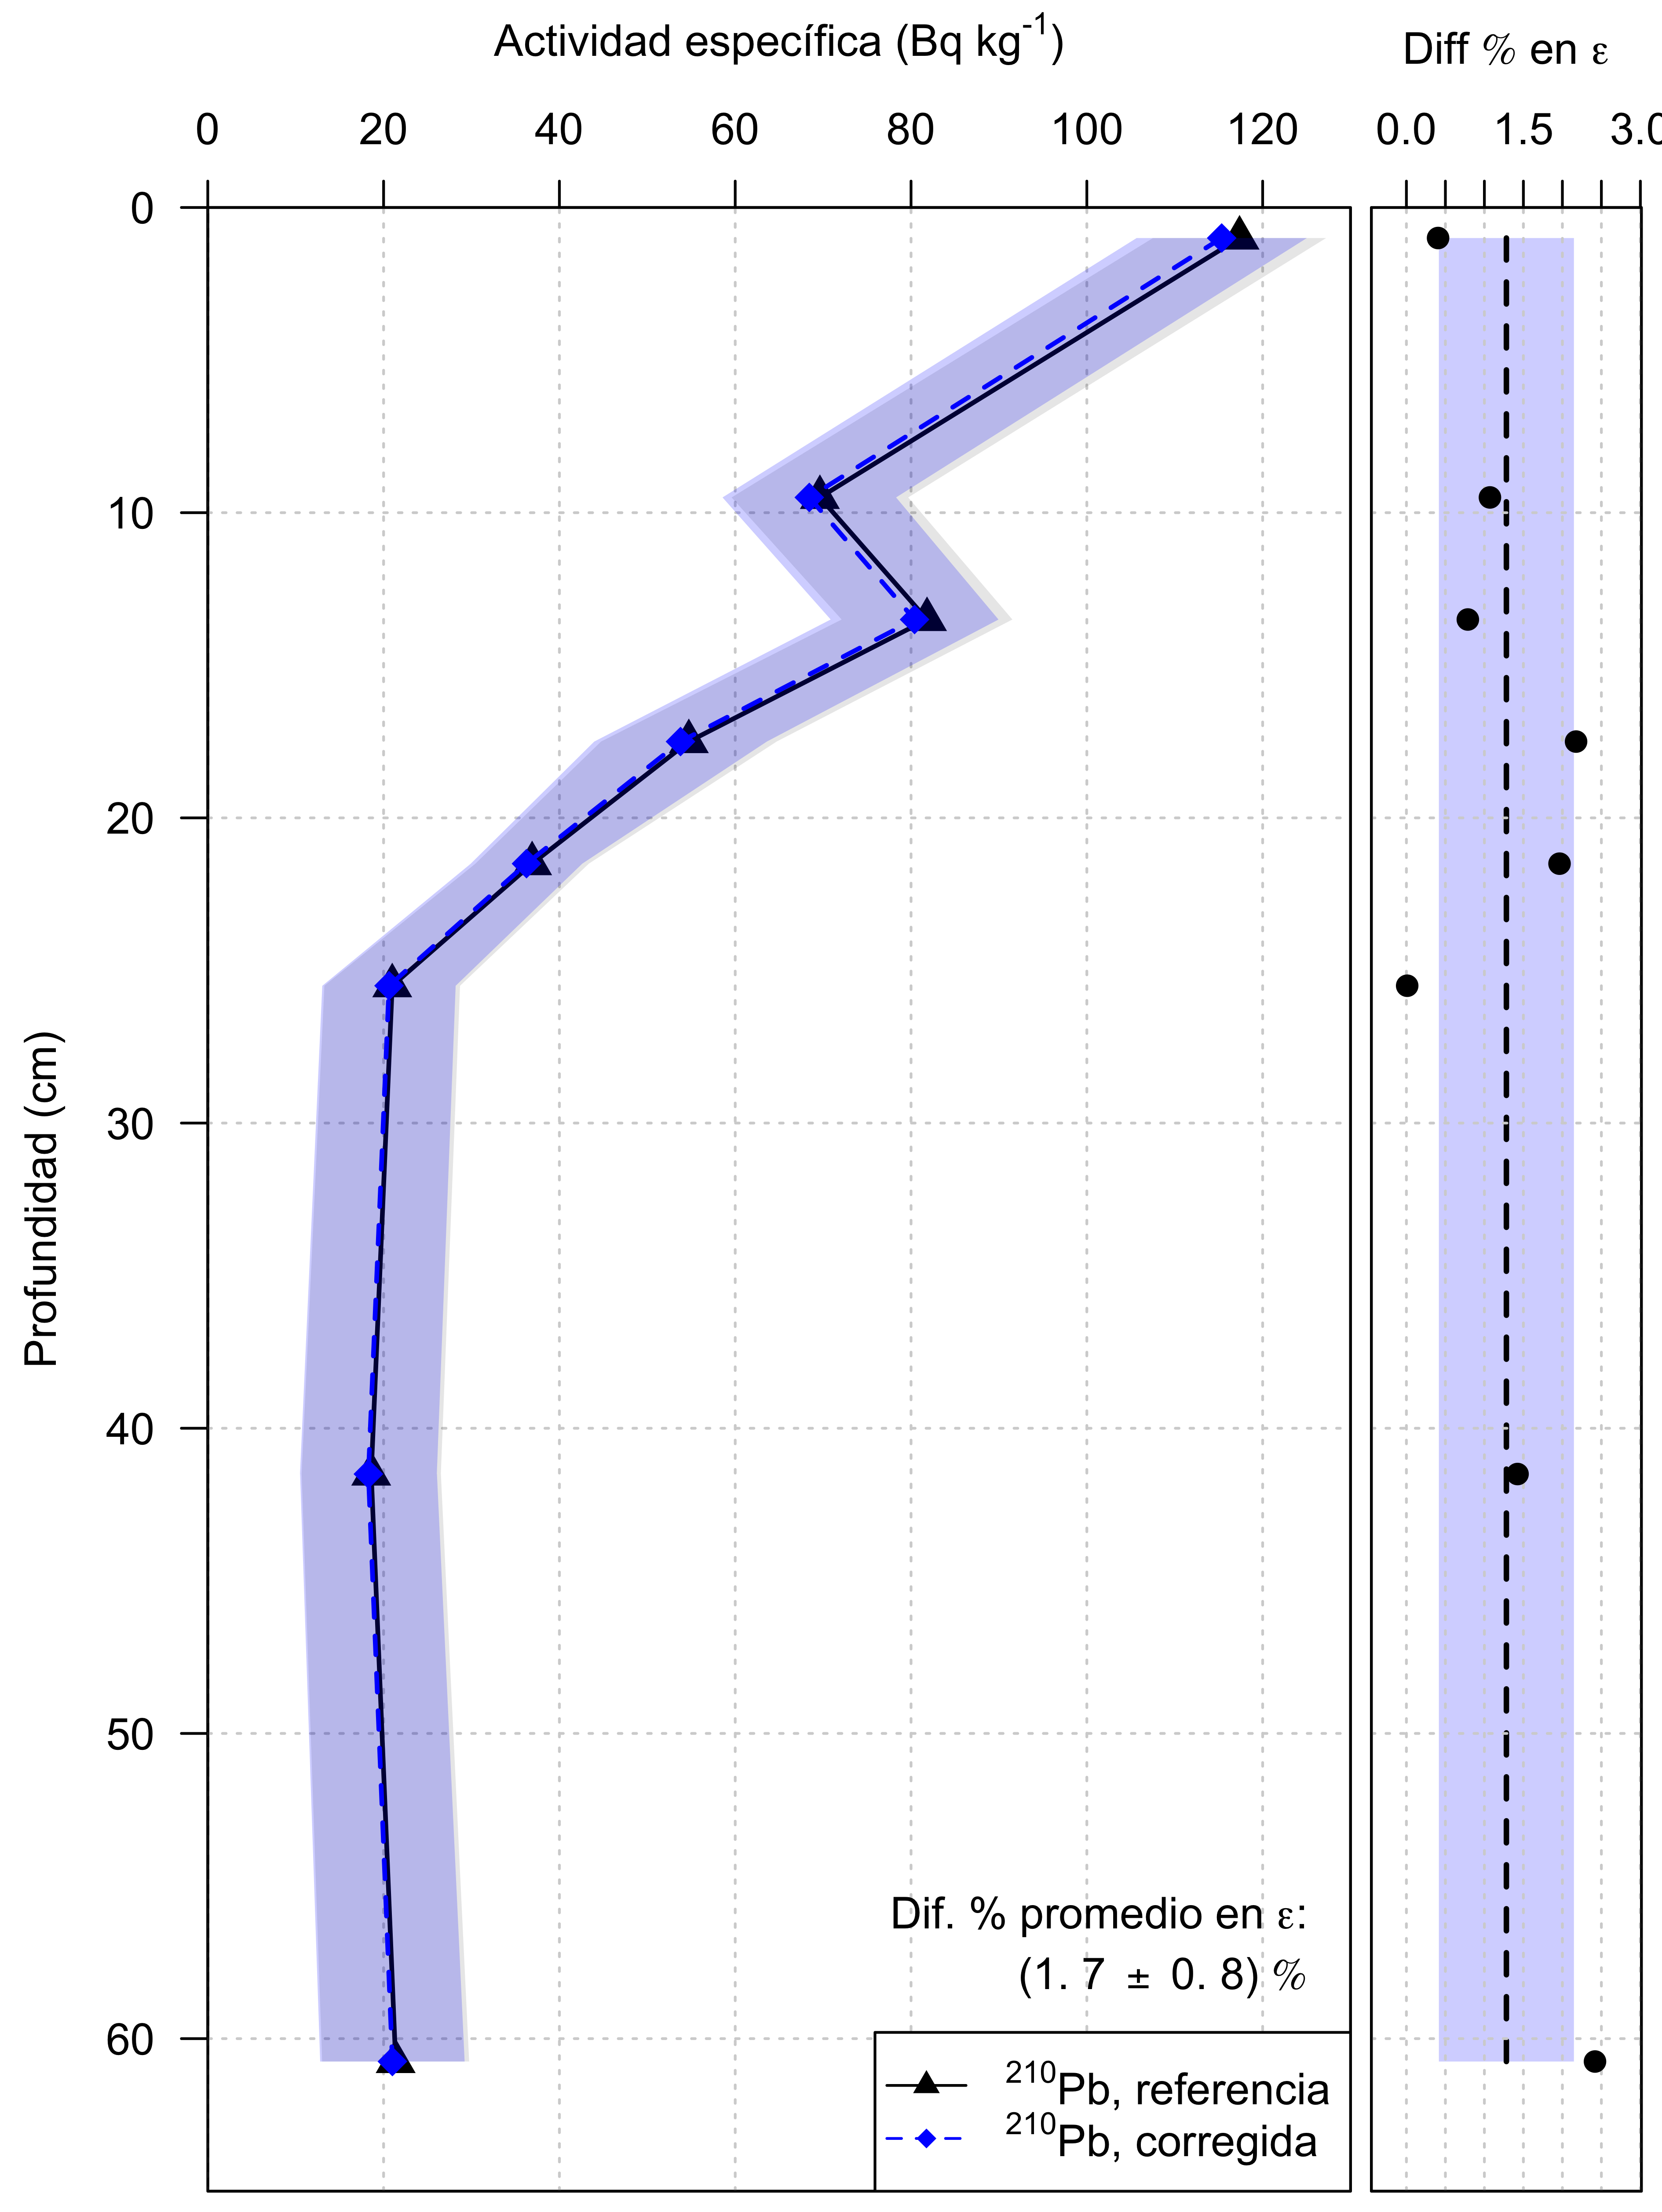
\includegraphics[width=0.9\textwidth]{Imagenes/Act_210Pb_Agua_Composicion_PCm.png}
\caption{Perfil de actividad específica de \PbCero\, para el núcleo \textbf{PCm} asumiendo una composición elemental de referencia y una composición corregida (Sección \ref{Secc-100Composicion}). Se muestra la diferencia porcentual promedio en el valor las eficiencias de referencia y corregida para una energía de 46.54 keV.}\label{FigPCmAgua}
\end{figure}
\begin{figure}
\centering
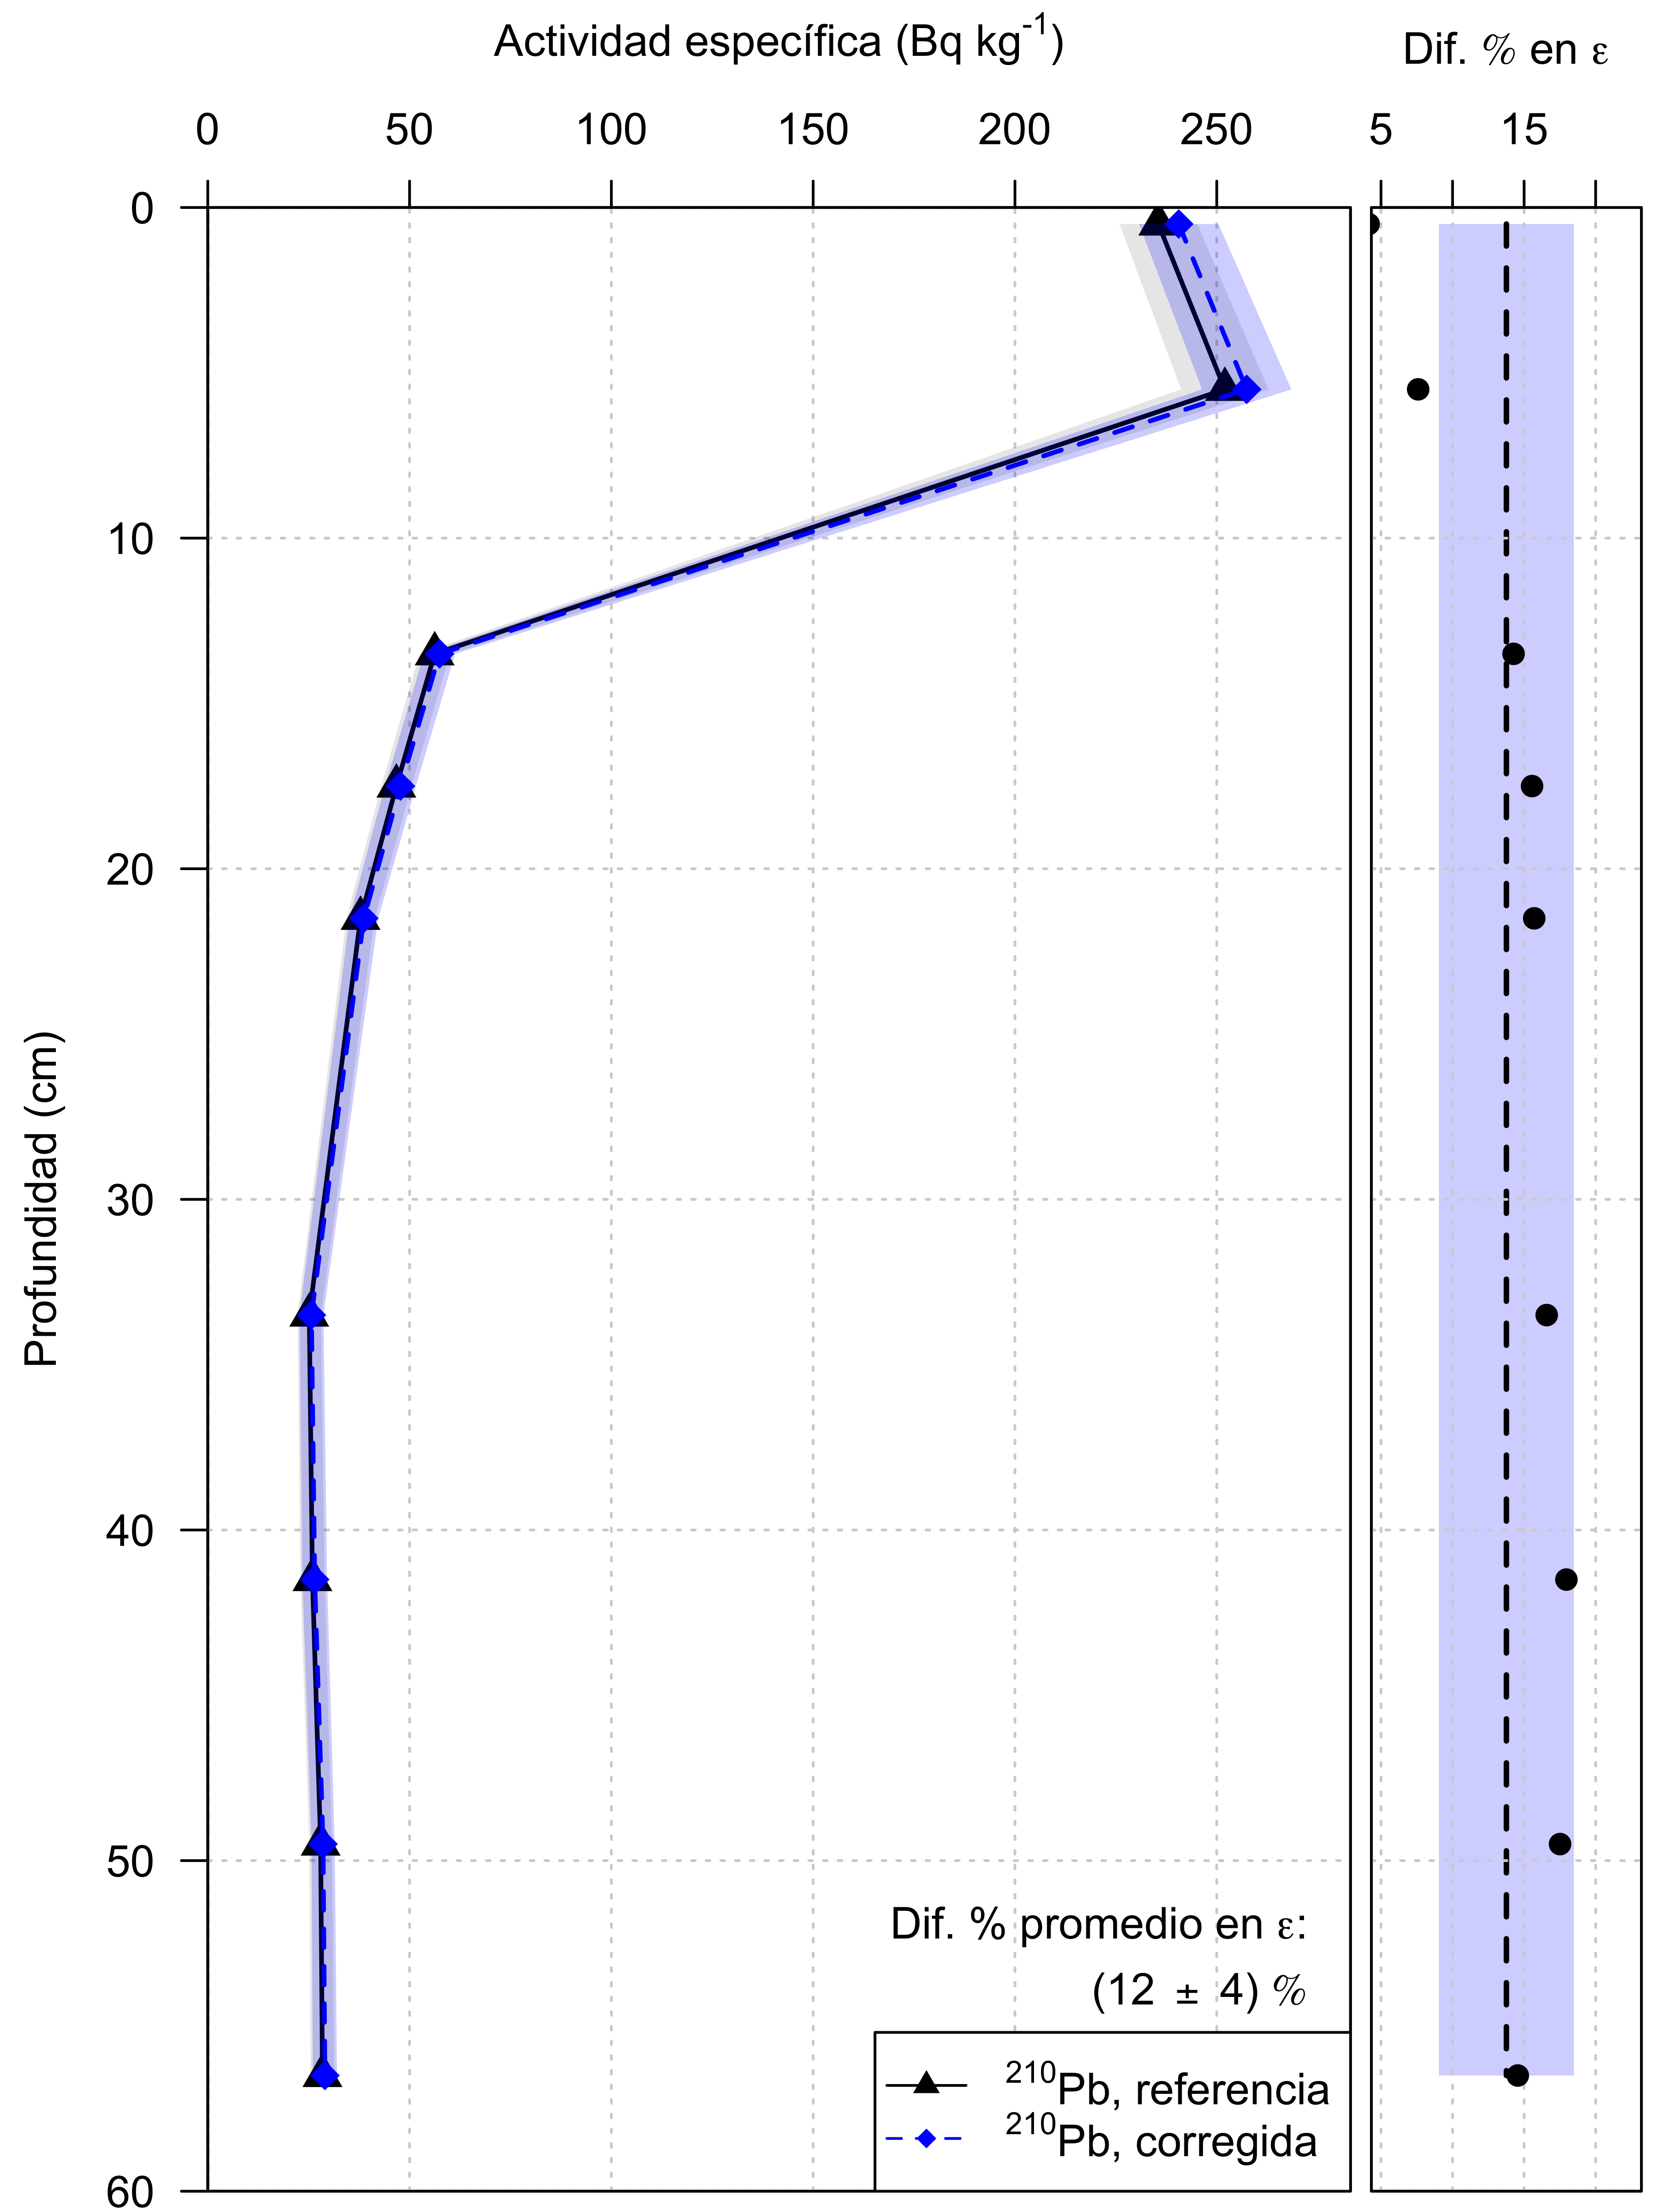
\includegraphics[width=0.9\textwidth]{Imagenes/Act_210Pb_Agua_Composicion_LTAF.png}
\caption{Perfil de actividad específica de \PbCero\, para el núcleo \textbf{LTAF} asumiendo una composición elemental de referencia y una composición corregida (Sección \ref{Secc-100Composicion}). Se muestra la diferencia porcentual promedio en el valor las eficiencias de referencia y corregida para una energía de 46.54 keV.}\label{FigLTAFAgua}
\end{figure}
\begin{figure}
\centering
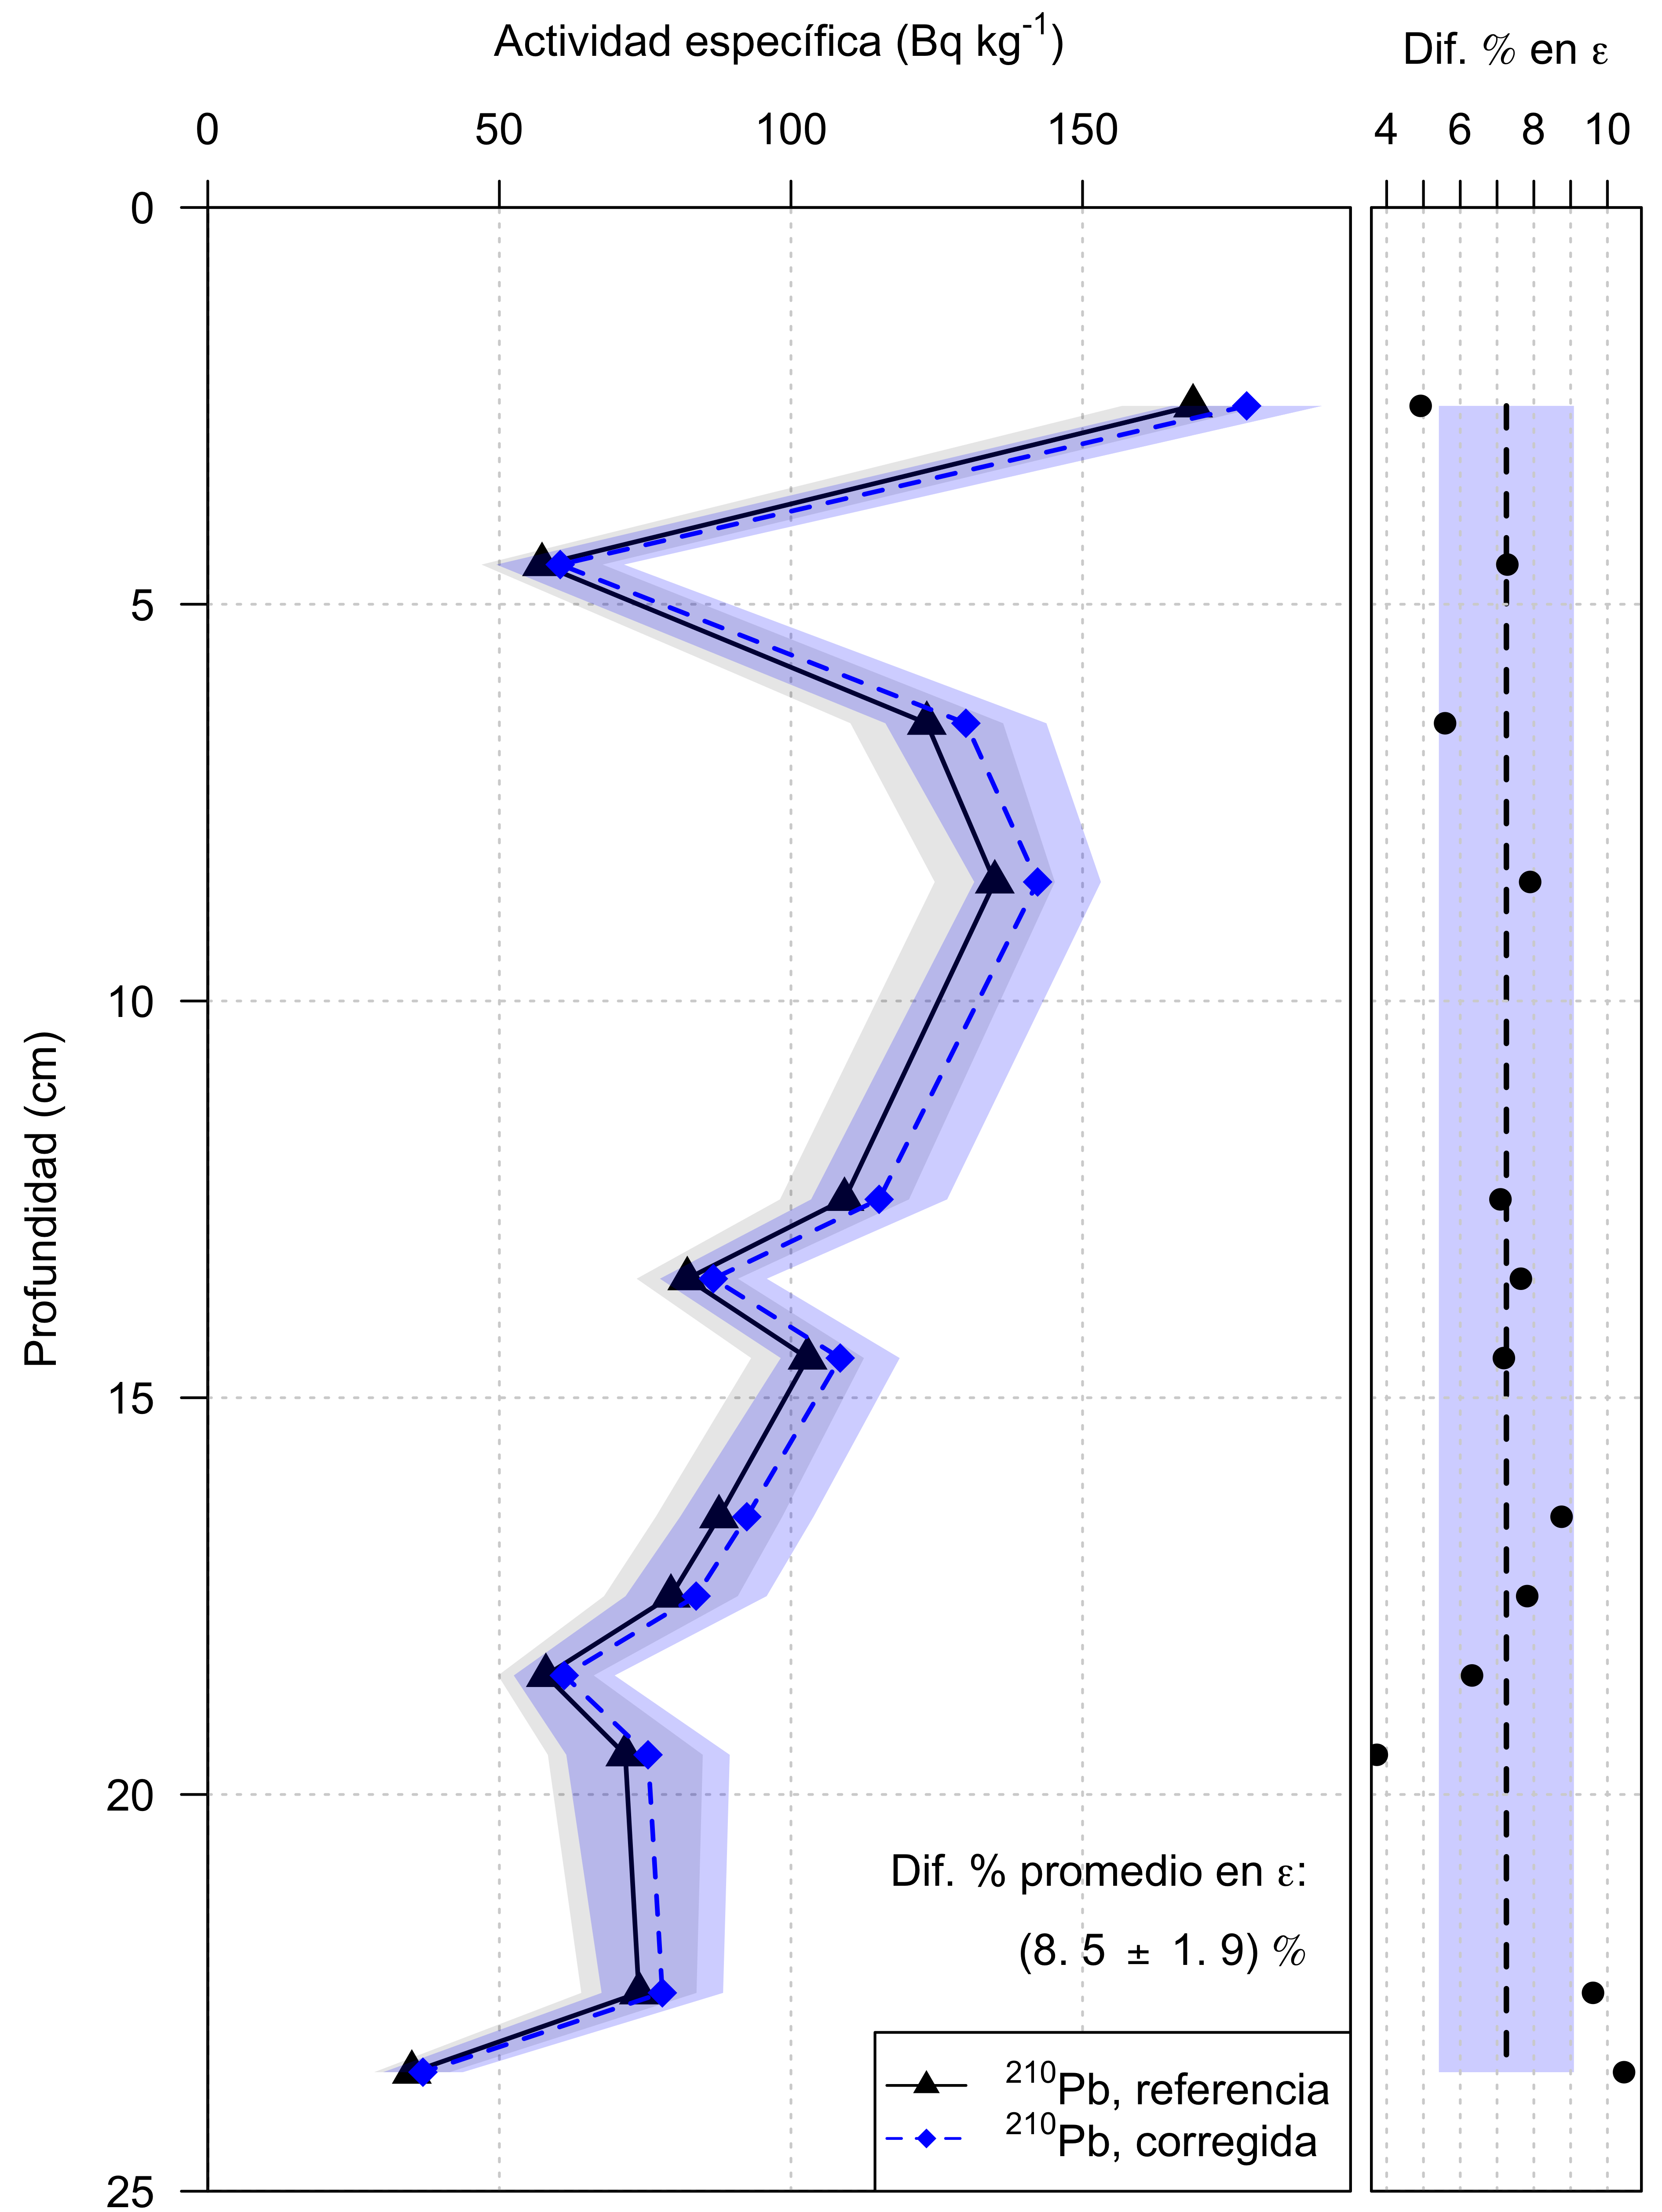
\includegraphics[width=0.9\textwidth]{Imagenes/Act_210Pb_Agua_Composicion_SAMO-14-2.png}
\caption{Perfil de actividad específica de \PbCero\, para el núcleo \textbf{SAMO-14-2} asumiendo una composición elemental de referencia y una composición corregida (Sección \ref{Secc-100Composicion}). Se muestra la diferencia porcentual promedio en el valor las eficiencias de referencia y corregida para una energía de 46.54 keV.}\label{FigSAMO142Agua}
\end{figure}
\begin{figure}
\centering
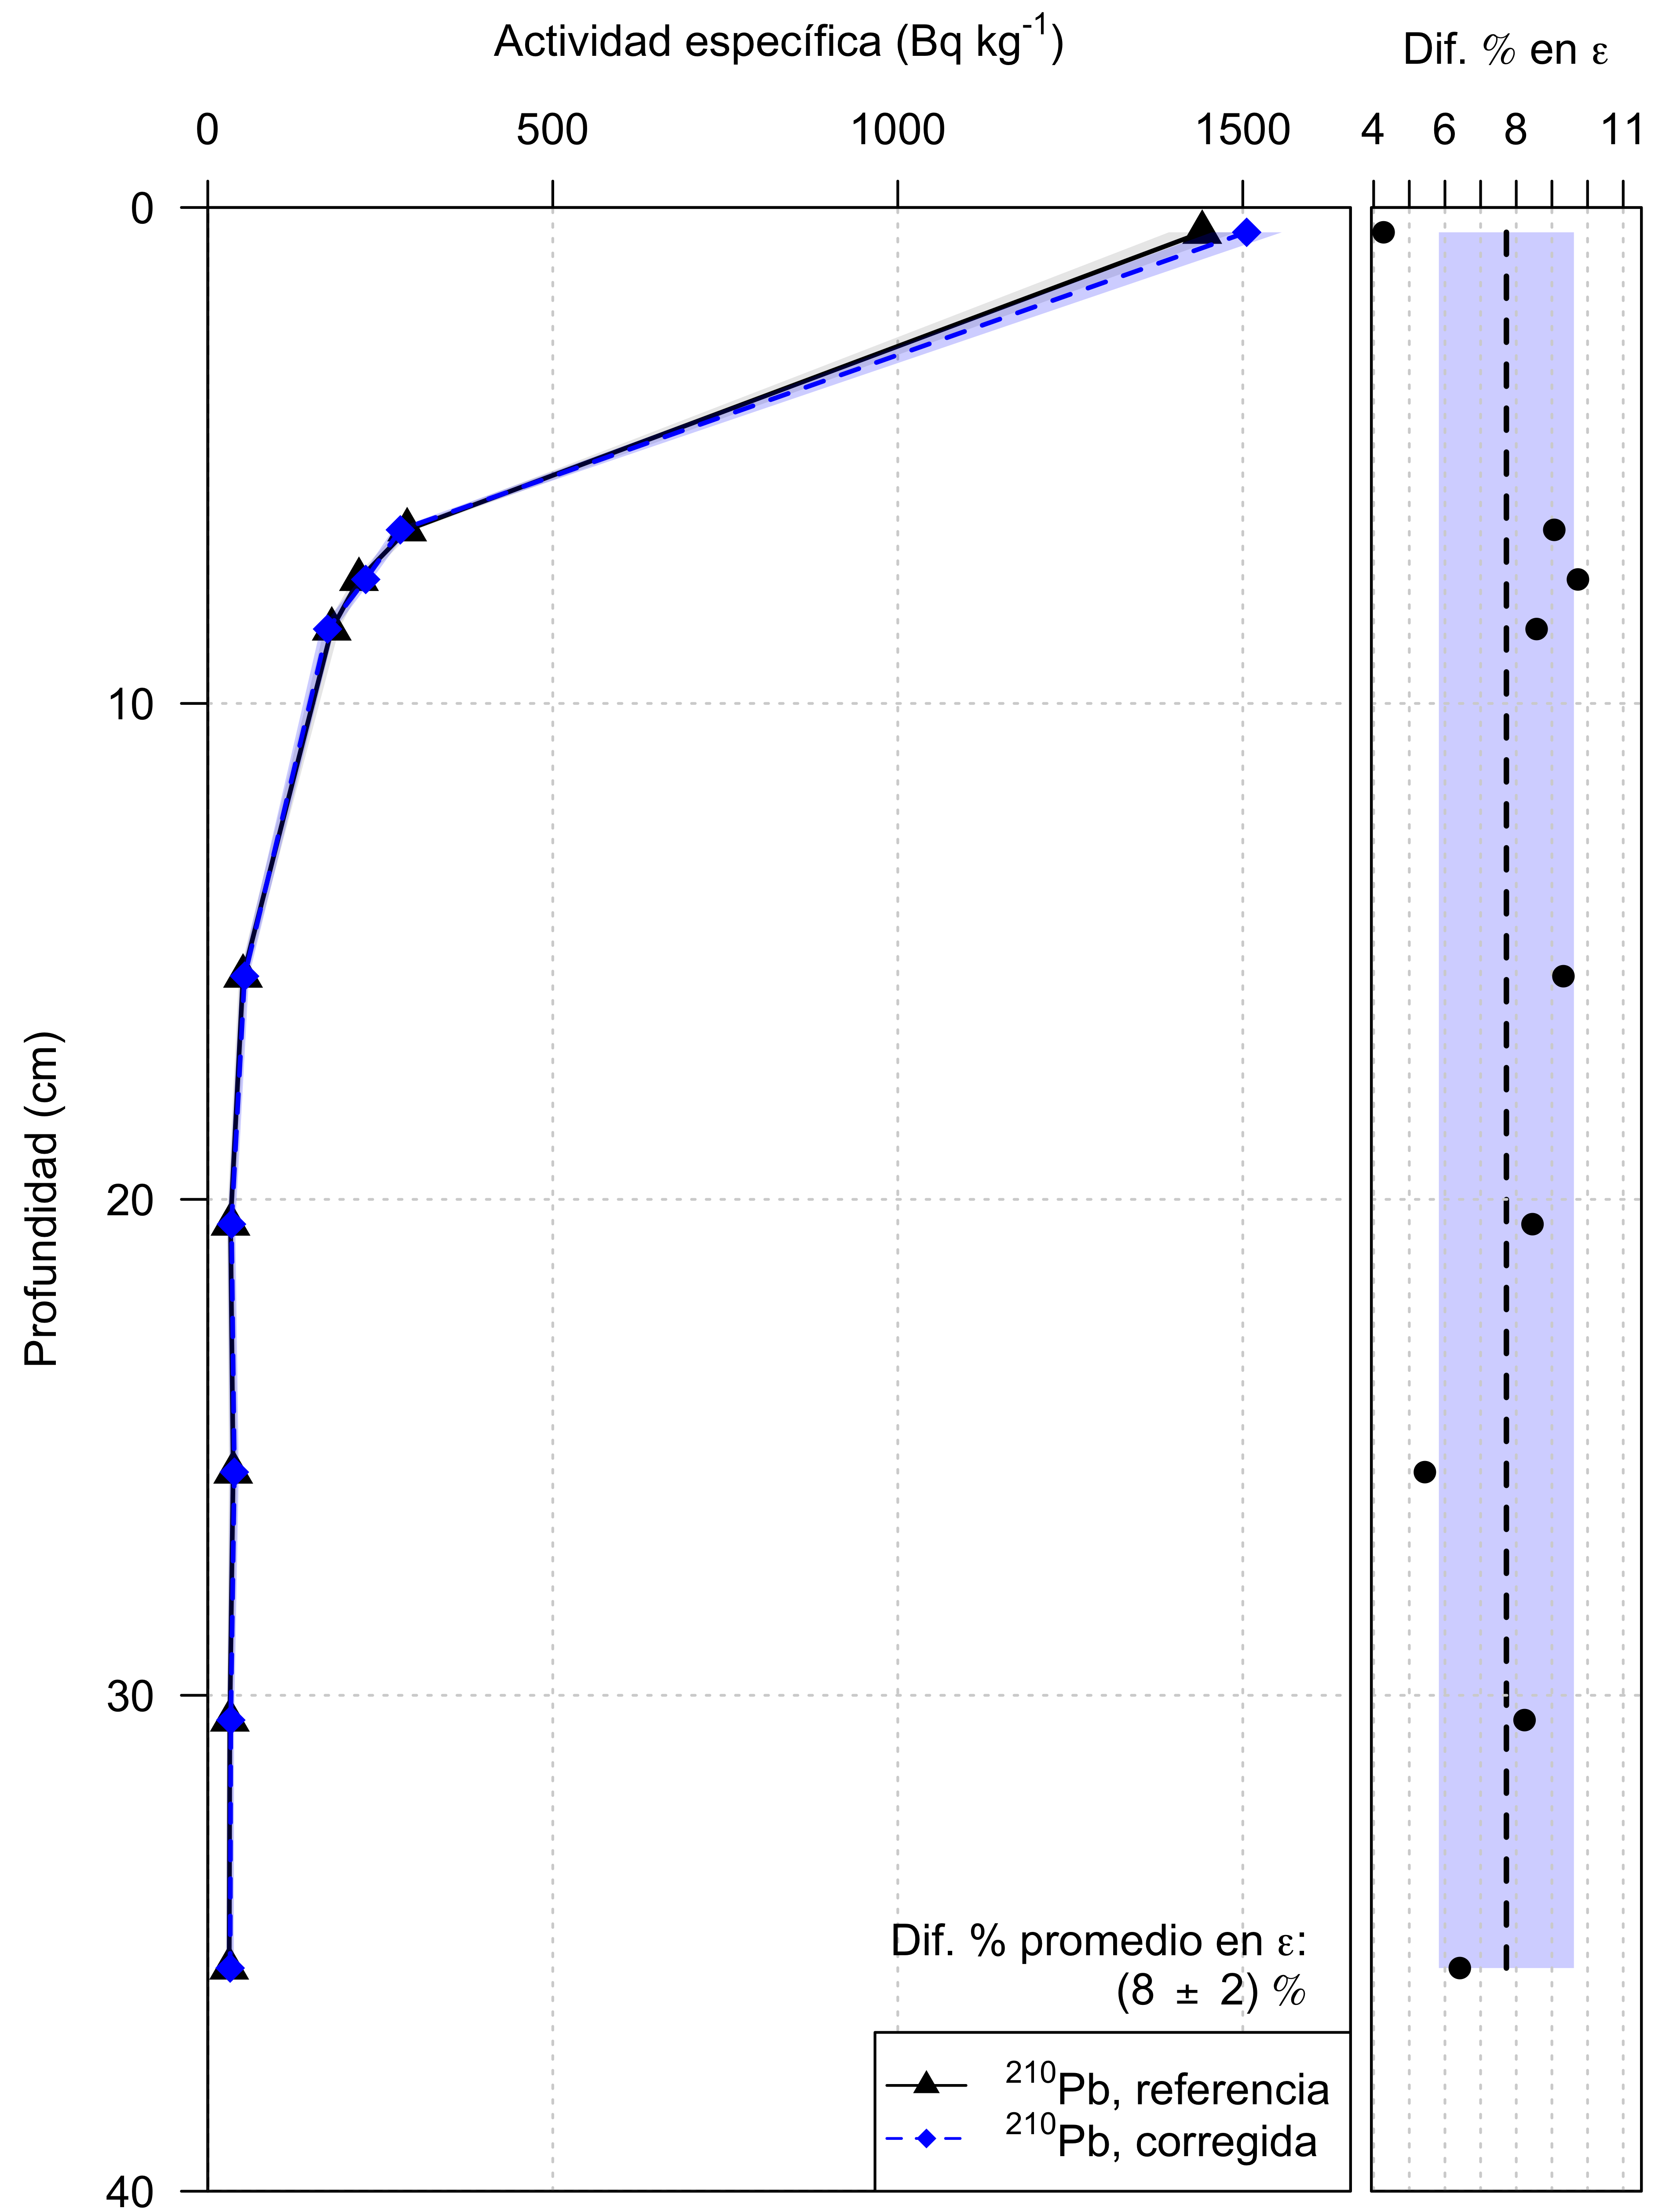
\includegraphics[width=0.9\textwidth]{Imagenes/Act_210Pb_Agua_Composicion_TEHUA-XII.png}
\caption{Perfil de actividad específica de \PbCero\, para el núcleo \textbf{TEHUA-XII} asumiendo una composición elemental de referencia y una composición corregida (Sección \ref{Secc-100Composicion}). Se muestra la diferencia porcentual promedio en el valor las eficiencias de referencia y corregida para una energía de 46.54 keV.}\label{FigTEHUAXIIAgua}
\end{figure}
\newpage
	\section{Equilibrio secular entre \PbCero\, y \PbCuatro}\label{Seccion-210y214}
Debido a la desintegración radiactiva en cadena de \UDosTresOcho\, y al tiempo de vida media de este radionúclido, se espera que los radionúclidos \PbCero\, y \PbCuatro\, se encuentren en equilibrio secular en las secciones más profundas (y por lo tanto más antiguas) de los núcleos sedimentarios. En el fechado con \PbCero\, esta es una información fundamental, pues define el alcance del modelo de fechado. Debido a las altas incertidumbres relativas de las medidas de bajas concentraciones, esta zona es a veces difícil de determinar. Por ejemplo, la última sección del núcleo sedimentario EU-VIII presenta una actividad específica de 2$20.2 \pm 5.8$  Bq kg$^{-1}$, por lo que la  incertidumbre relativa es de un 29 \%. 
\\
\\
En las Figuras \ref{Fig-EUVIII-Comp}, \ref{Fig-GOMRI500-Comp}, \ref{Fig-PCm-Comp}, \ref{Fig-LTAF-Comp}, \ref{Fig-SAMO142-Comp} y \ref{Fig-TEHUAXII-Comp} se muestran los perfiles corregidos de \PbCero\, y \PbCuatro\, y las secciones que posiblemente se encuentran en equilibrio secular. Los rangos de actividad específica y profundidad de los anterior perfiles varían entre núcleos sedimentarios.
\\
\\
De las zonas de manglar, las actividades de las tres últimas secciones medidas en el núcleo sedimentario EU-VIII fueron similares (dentro de las incertidumbres de medida). Sin embargo, en el núcleo PCm, las actividades de \PbCero\, fueron aparentemente superiores a las de \PbCuatro, aunque las incertidumbres se sobreponen y, por lo tanto, podemos considerar que se ha alcanzado el equilibrio secular. 
\\
\\
Un comportamiento inverso fue observado en el núcleo LTAF, pues las actividades de \PbCero\, son en este caso inferiores al \PbCuatro, lo que significa la presencia de un déficit de \PbCero, probablemente  debido a un enriquecimiento de \Ra\, (en equilibrio con el \PbCuatro) debido a procesos diagenéticos. De hecho, LTAF es el núcleo sedimentario de manglar con mayor concentración de \PbCero, que puede ser debido a la migración hacia la superficie de \Ra<  \, de capas inferiores, causando así su exceso respecto al \PbCero. Esto es consistente con el decrecimiento del \PbCuatro\, en las capas superficiales, indicando que parte del \Ra\, está siendo transferido al agua intersticial, y de aquí a la columna de agua. En estos casos, es recomendable utilizar las concentraciones de \PbCero\, en el fondo del núcleo para estimar un valor constante del \PbCeroEx. 
\\
\\
En este caso, se asigna que las 4 últimas secciones medidas del núcleo LTAF pertenecen a la zona de equilibrio secular con un valor promedio de las actividades específicas de \PbCero\, de $31.6 \pm 9.9$ Bq kg$^{-1}$ (coeficiente de variación del 31 \%) y un valor promedio de las actividades específicas de \PbCuatro\, de $40.0 \pm 12.1$ Bq kg$^{-1}$ (coeficiente de variación del 30 \%). Utilizando el test estadístico $Z$ (o método $Z$-score), inferimos que estas distribuciones no son diferentes ($p$ < 0.05). 
\\
\\
Los núcleos de mar abierto fueron los que mostraron una mayor corrección de eficiencia. En el núcleo sedimentario GOMRI-500 las concentraciones de \PbCero\, fueron algo superiores que las de \PbCuatro, pero dentro de las incertidumbres en dos de las tres secciones. Contrariamente, las concentraciones de \PbCero\, fueron algo inferiores a las de \PbCuatro\, en el núcleo TEHUA-XII, si bien todas las secciones mostraron equilibrio secular dentro de las incertidumbres. Por lo tanto concluimos que en ambos casos se llegó al equilibrio secular. En el caso del núcleo sedimentario GOMRI-500 se observó una zona de equilibrio en la mitad del núcleo, que muy probablemente indica el registro de un evento natural o antropogénico, cuya discusión está fuera del alcance de este trabajo. Para el núcleo lacustre SAMO-14-2, tan sólo una de las secciones medidas está en la zona de equilibrio, si bien las concentraciones son prácticamente idénticas, por lo que concluimos que se llegó a la zona de equilibrio secular. 
\\
\\
Para cuantificar estas observaciones empíricas, se definió la variable $\delta$ (ver Figura \ref{Fig-DiffPorcentualEquilibrio}) como la diferencia porcentual  de  la  actividad  específica  de  \PbCero\, respecto a la actividad específica de \PbCuatro\, para las secciones que se encuentran en la zona de equilibrio secular, 
\begin{equation}
\delta = \dfrac{A(^{214}\text{Pb}) - A(^{210}\text{Pb}) }{A(^{214}\text{Pb}) } \times 100.
\end{equation}
En el Apéndice \ref{ApexZonaEquilibrio} se muestran las secciones de los núcleos sedimentarios en donde se asume equilibrio secular, aquellas en donde las actividades corregidas de \PbCero\, y \PbCuatro\, se superponen al incluir las incertidumbres. Utilizando las secciones pertenecientes a la zona de equilibrio (37.5 cm, 45.5 cm y 53.5 cm del núcleo EU-VIII, 12.25 cm y 21.75 cm del núcleo GOMRI-500 y la sección 23.5 cm del SAMO-14-2), se obtuvo un valor promedio de $\overline{\delta} = 7 \pm 8$, que incluye al cero y confirma que los criterios utilizados para detectar la presencia de equilibrio secular son correctas. Cabe resaltar que las desviaciones $\delta$ para algunas secciones pertenecientes a la zona de equilibrio son en algunos casos altas y que éstas pueden ser debidas a razones geoquímicas y no de calibración de los sistemas de espectrometría de rayos gamma. 
\begin{figure}
\centering
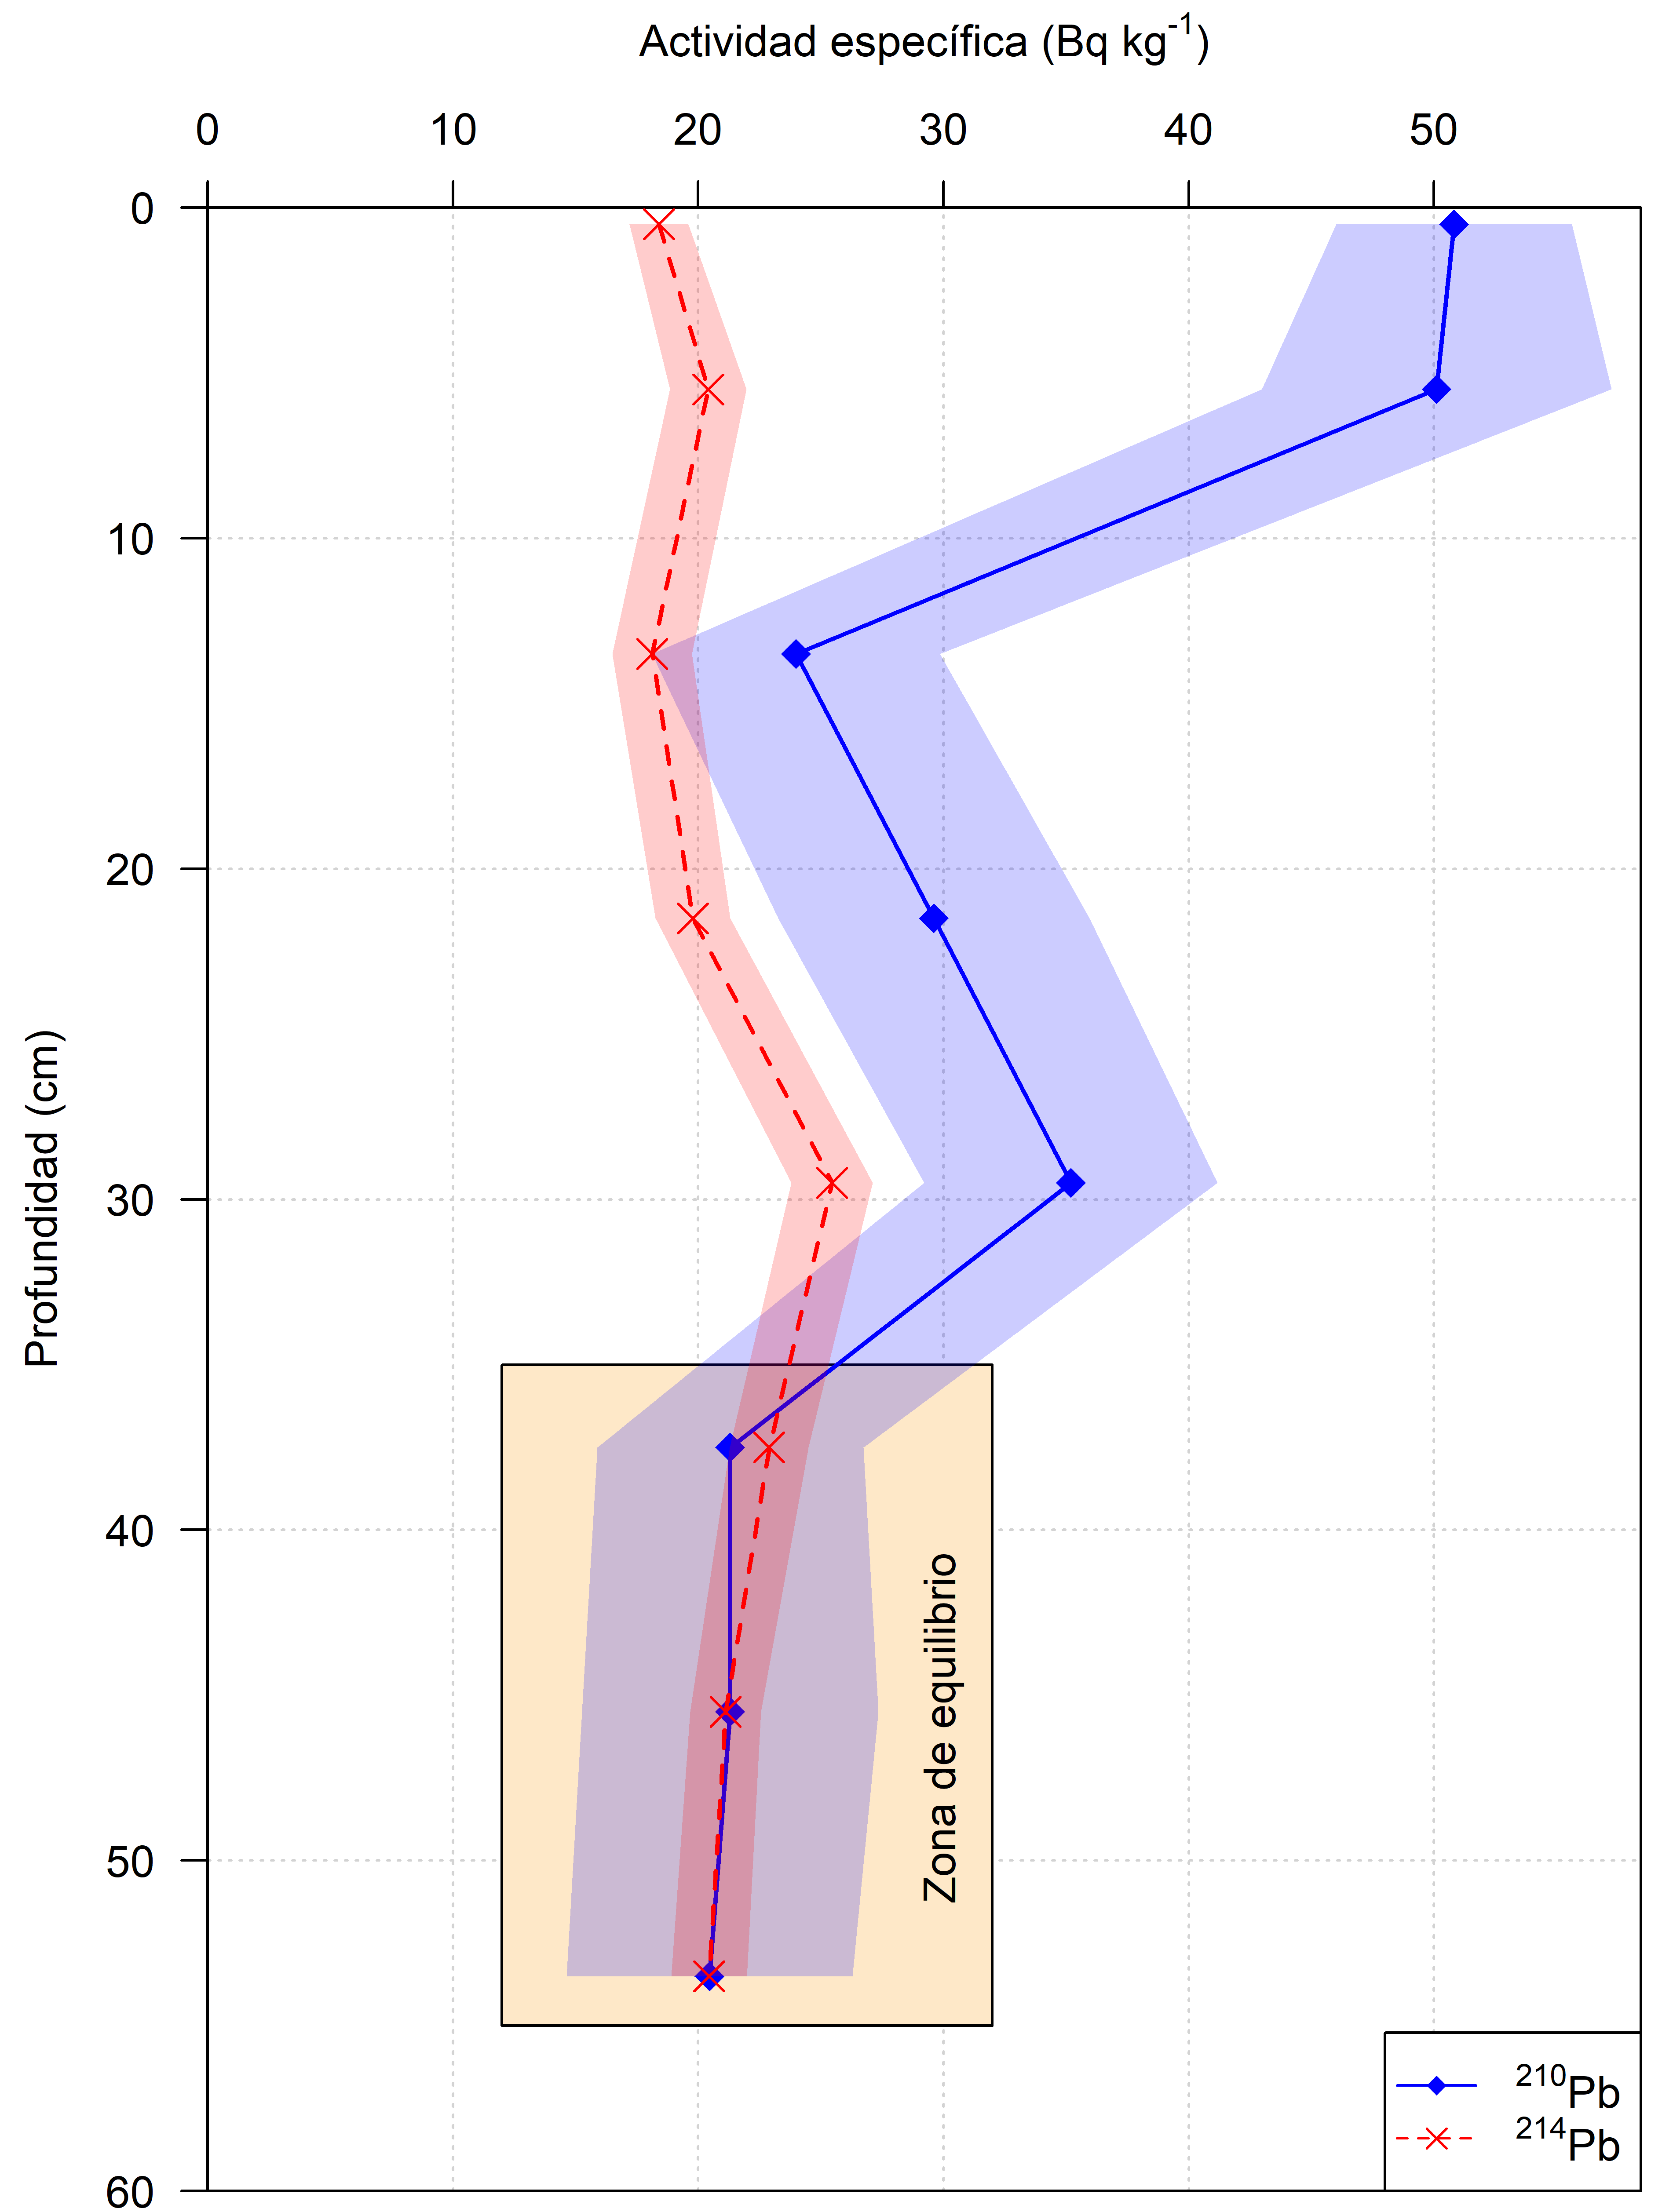
\includegraphics[width=0.9\textwidth]{Imagenes/Act_210Pb_214Pb_EU_VIII.png}
\caption{Perfiles de actividad específica de \PbCero\, y \PbCuatro\,corregidos para el núcleo sedimentario \textbf{EU-VIII}. Las tres últimas secciones posiblemente se encuentran en equilibrio secular.}\label{Fig-EUVIII-Comp}
\end{figure}
\begin{figure}
\centering
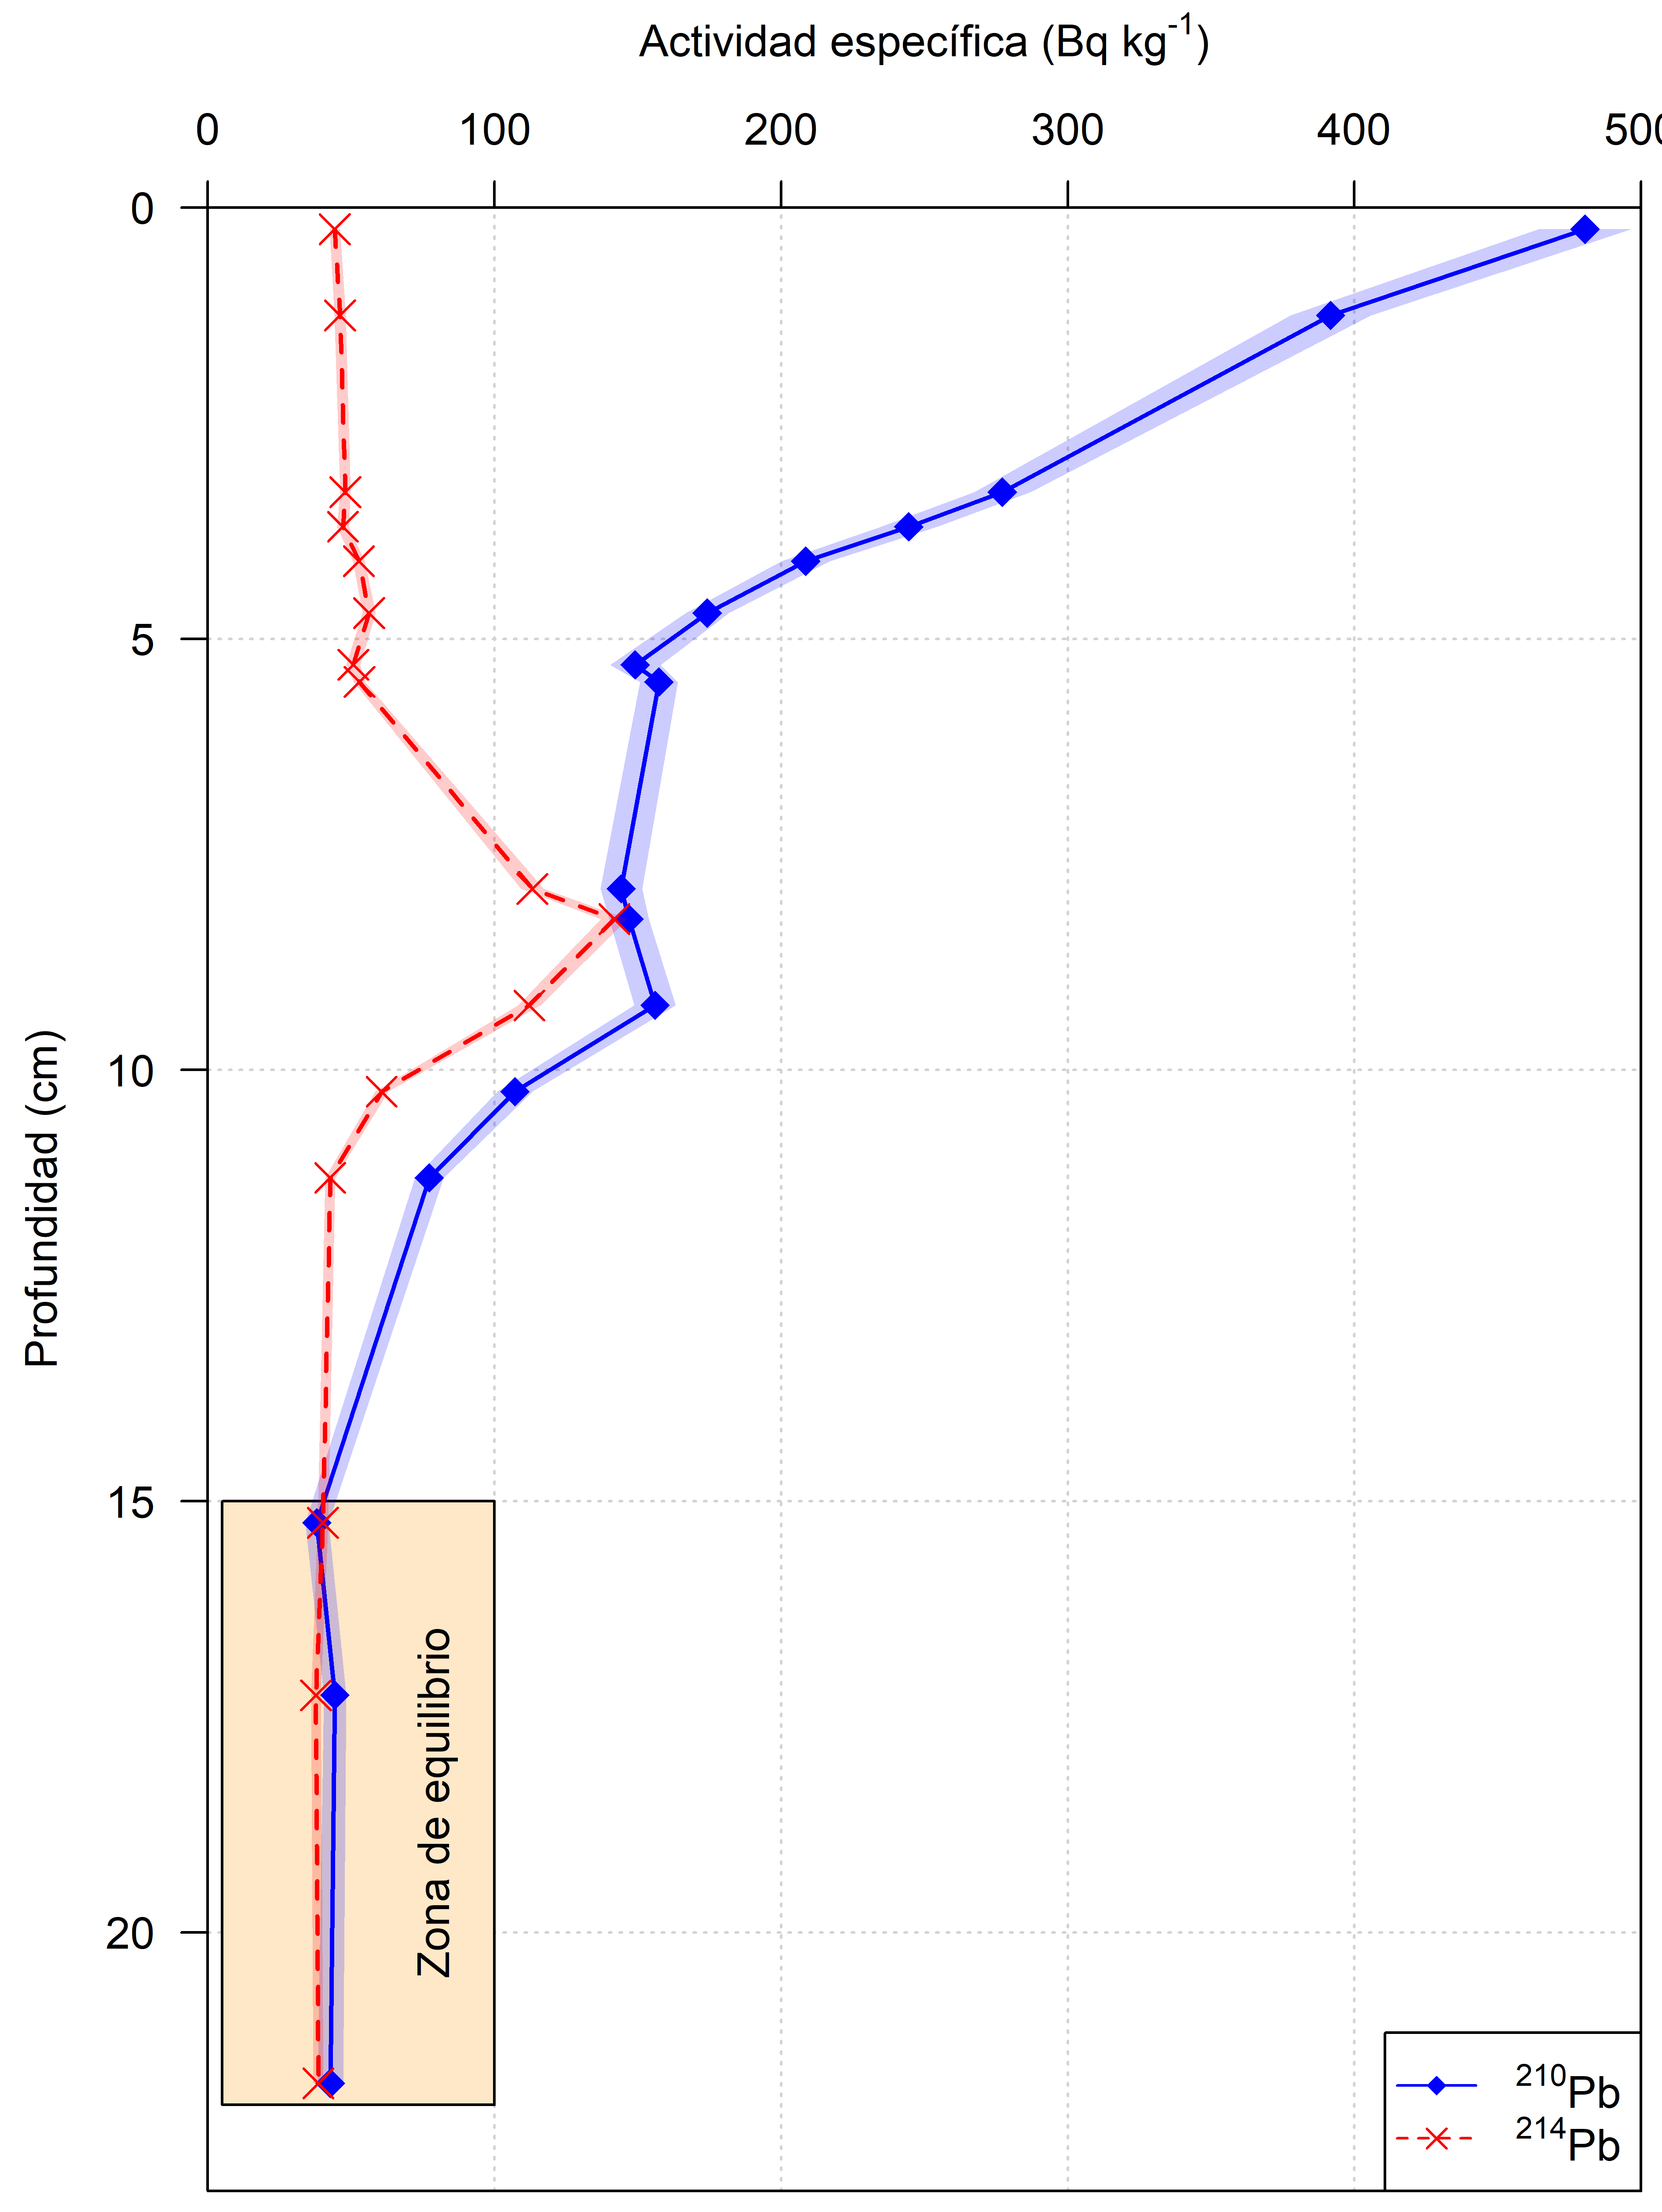
\includegraphics[width=0.9\textwidth]{Imagenes/Act_210Pb_214Pb_GOMRI_500.png}
\caption{Perfiles de actividad específica de \PbCero\, y \PbCuatro\, corregidos para el núcleo sedimentario \textbf{GOMRI-500}. Las tres últimas secciones posiblemente se encuentran en equilibrio secular.}\label{Fig-GOMRI500-Comp}
\end{figure}
\begin{figure}
\centering
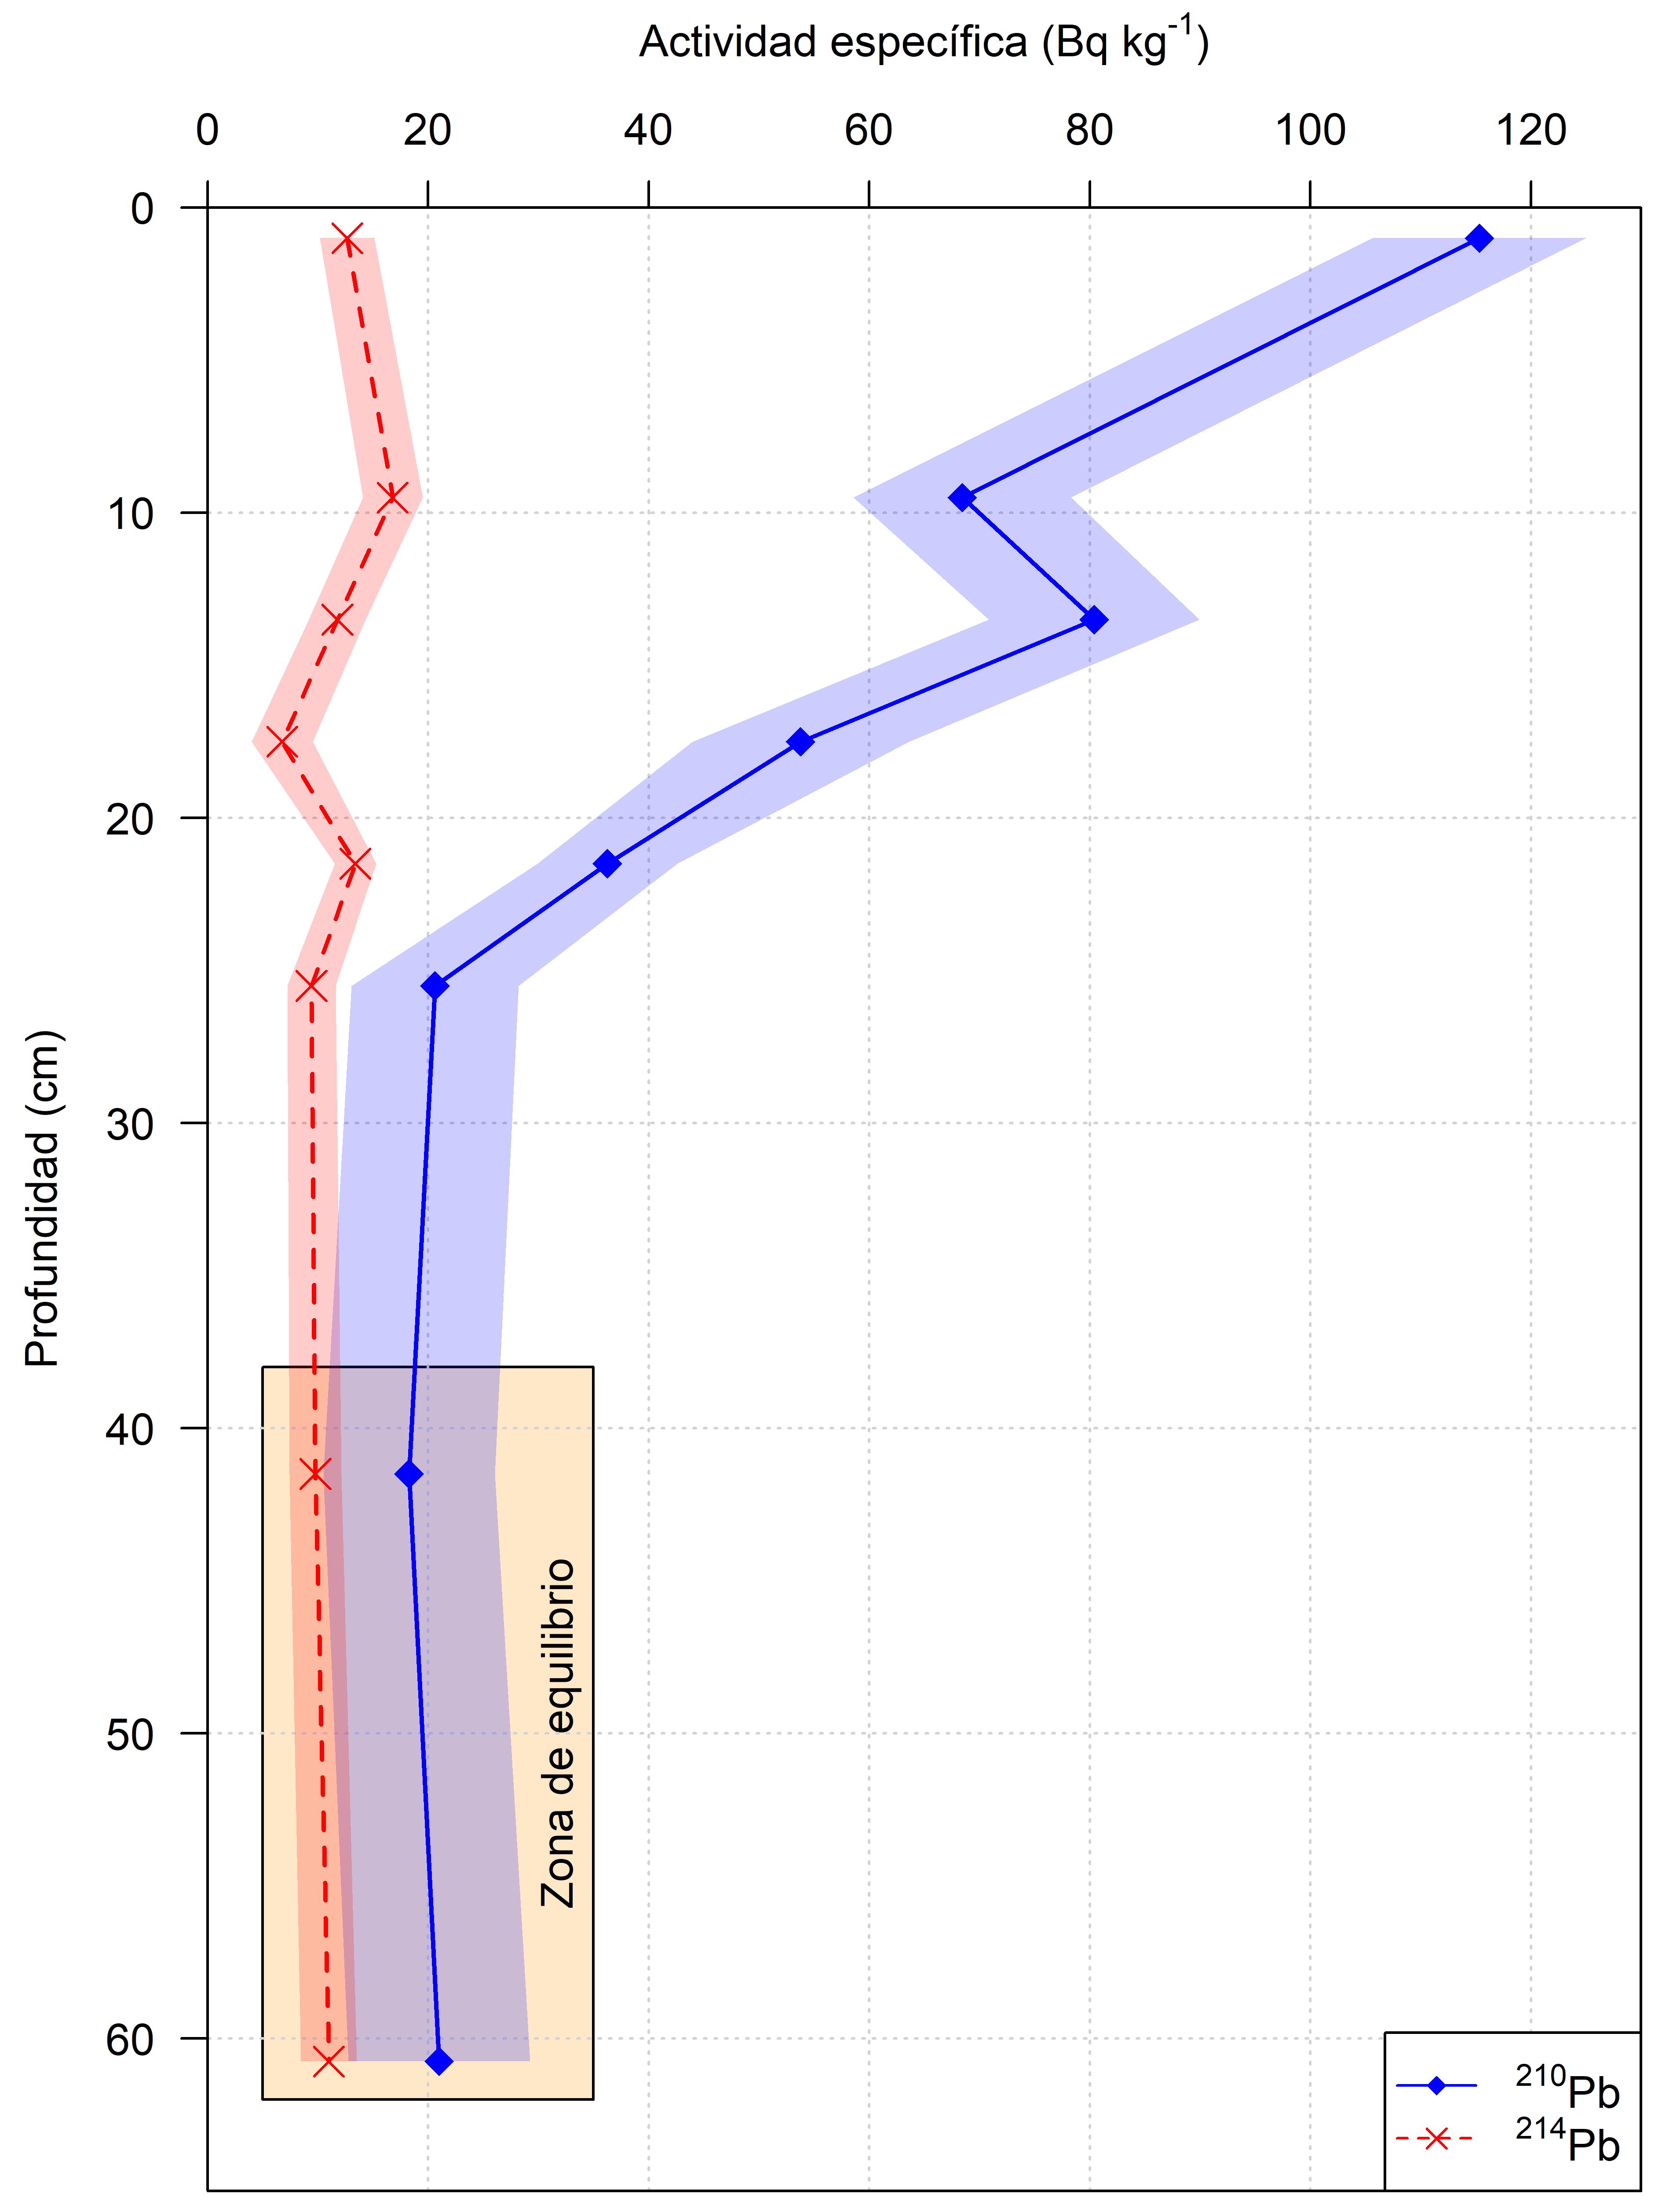
\includegraphics[width=0.9\textwidth]{Imagenes/Act_210Pb_214Pb_PCm.png}
\caption{Perfiles de actividad específica de \PbCero\, y \PbCuatro\,corregidos para el núcleo sedimentario \textbf{PCm}. Las dos últimas secciones posiblemente se encuentran en equilibrio secular.}\label{Fig-PCm-Comp}
\end{figure}
\begin{figure}
\centering
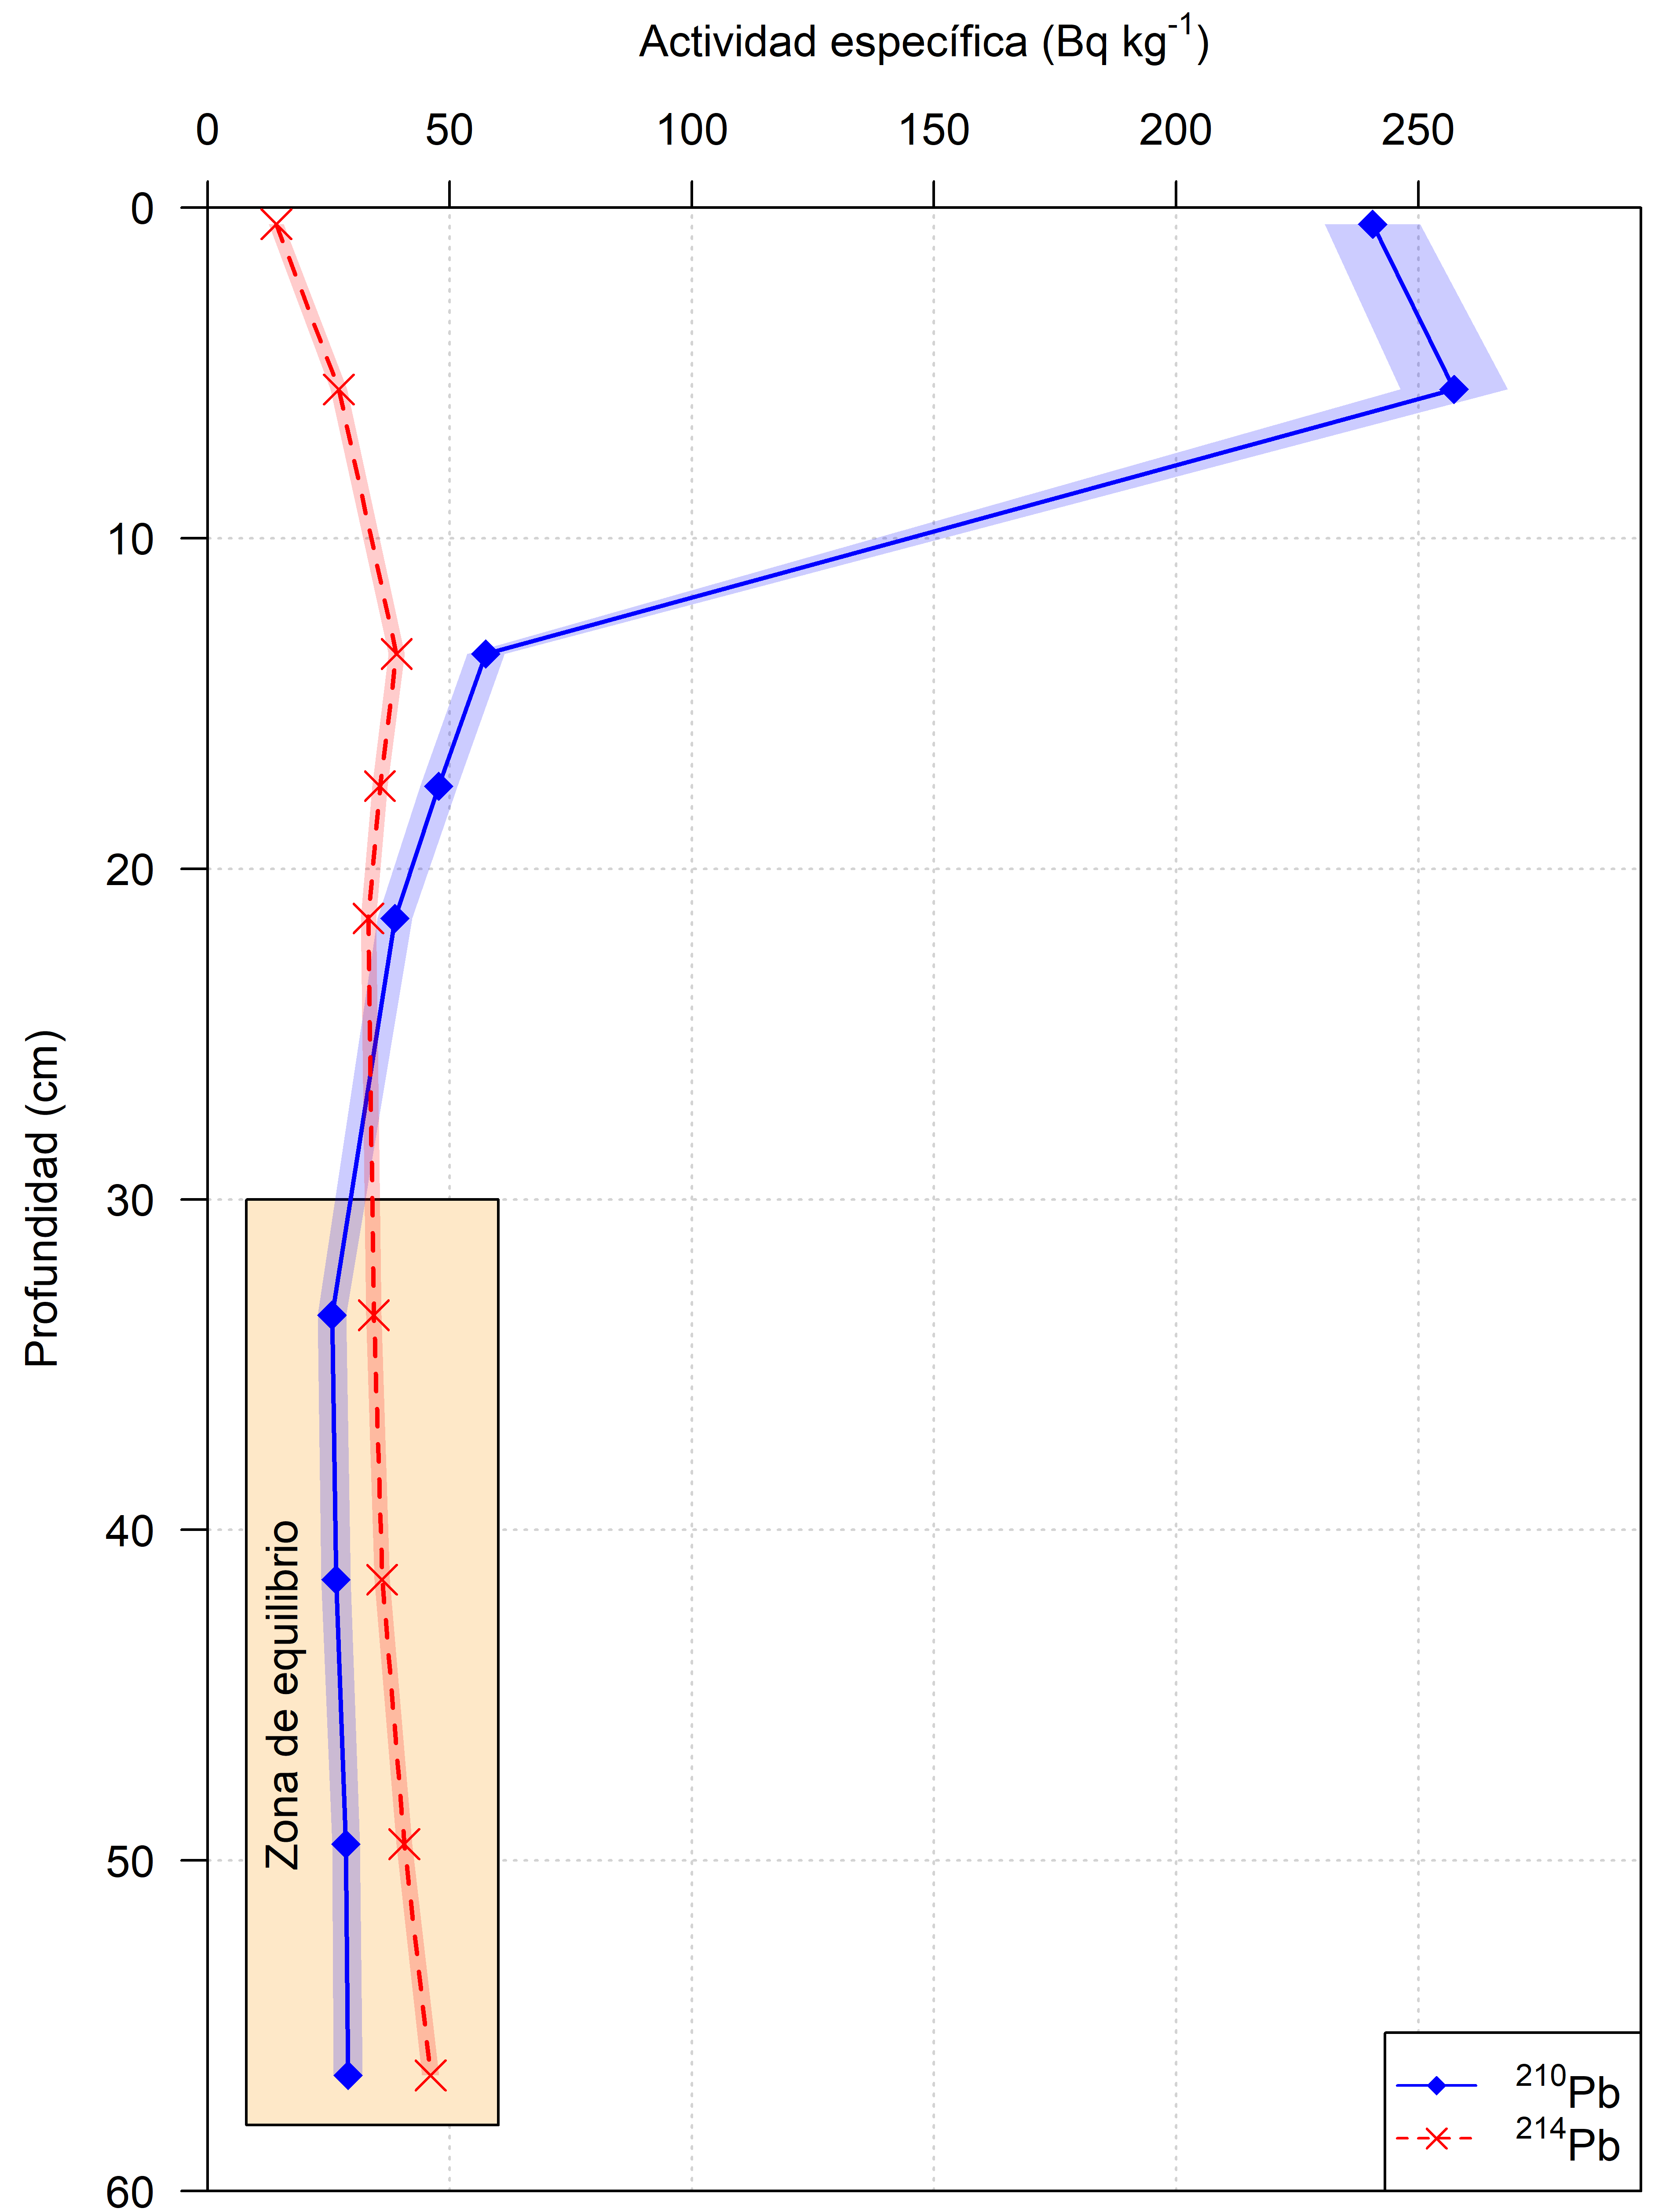
\includegraphics[width=0.9\textwidth]{Imagenes/Act_210Pb_214Pb_LTAF.png}
\caption{Perfiles de actividad específica de \PbCero\, y \PbCuatro\,corregidos para el núcleo sedimentario \textbf{LTAF}. Las tres últimas secciones posiblemente se encuentran en equilibrio secular.}\label{Fig-LTAF-Comp}
\end{figure}
\begin{figure}
\centering
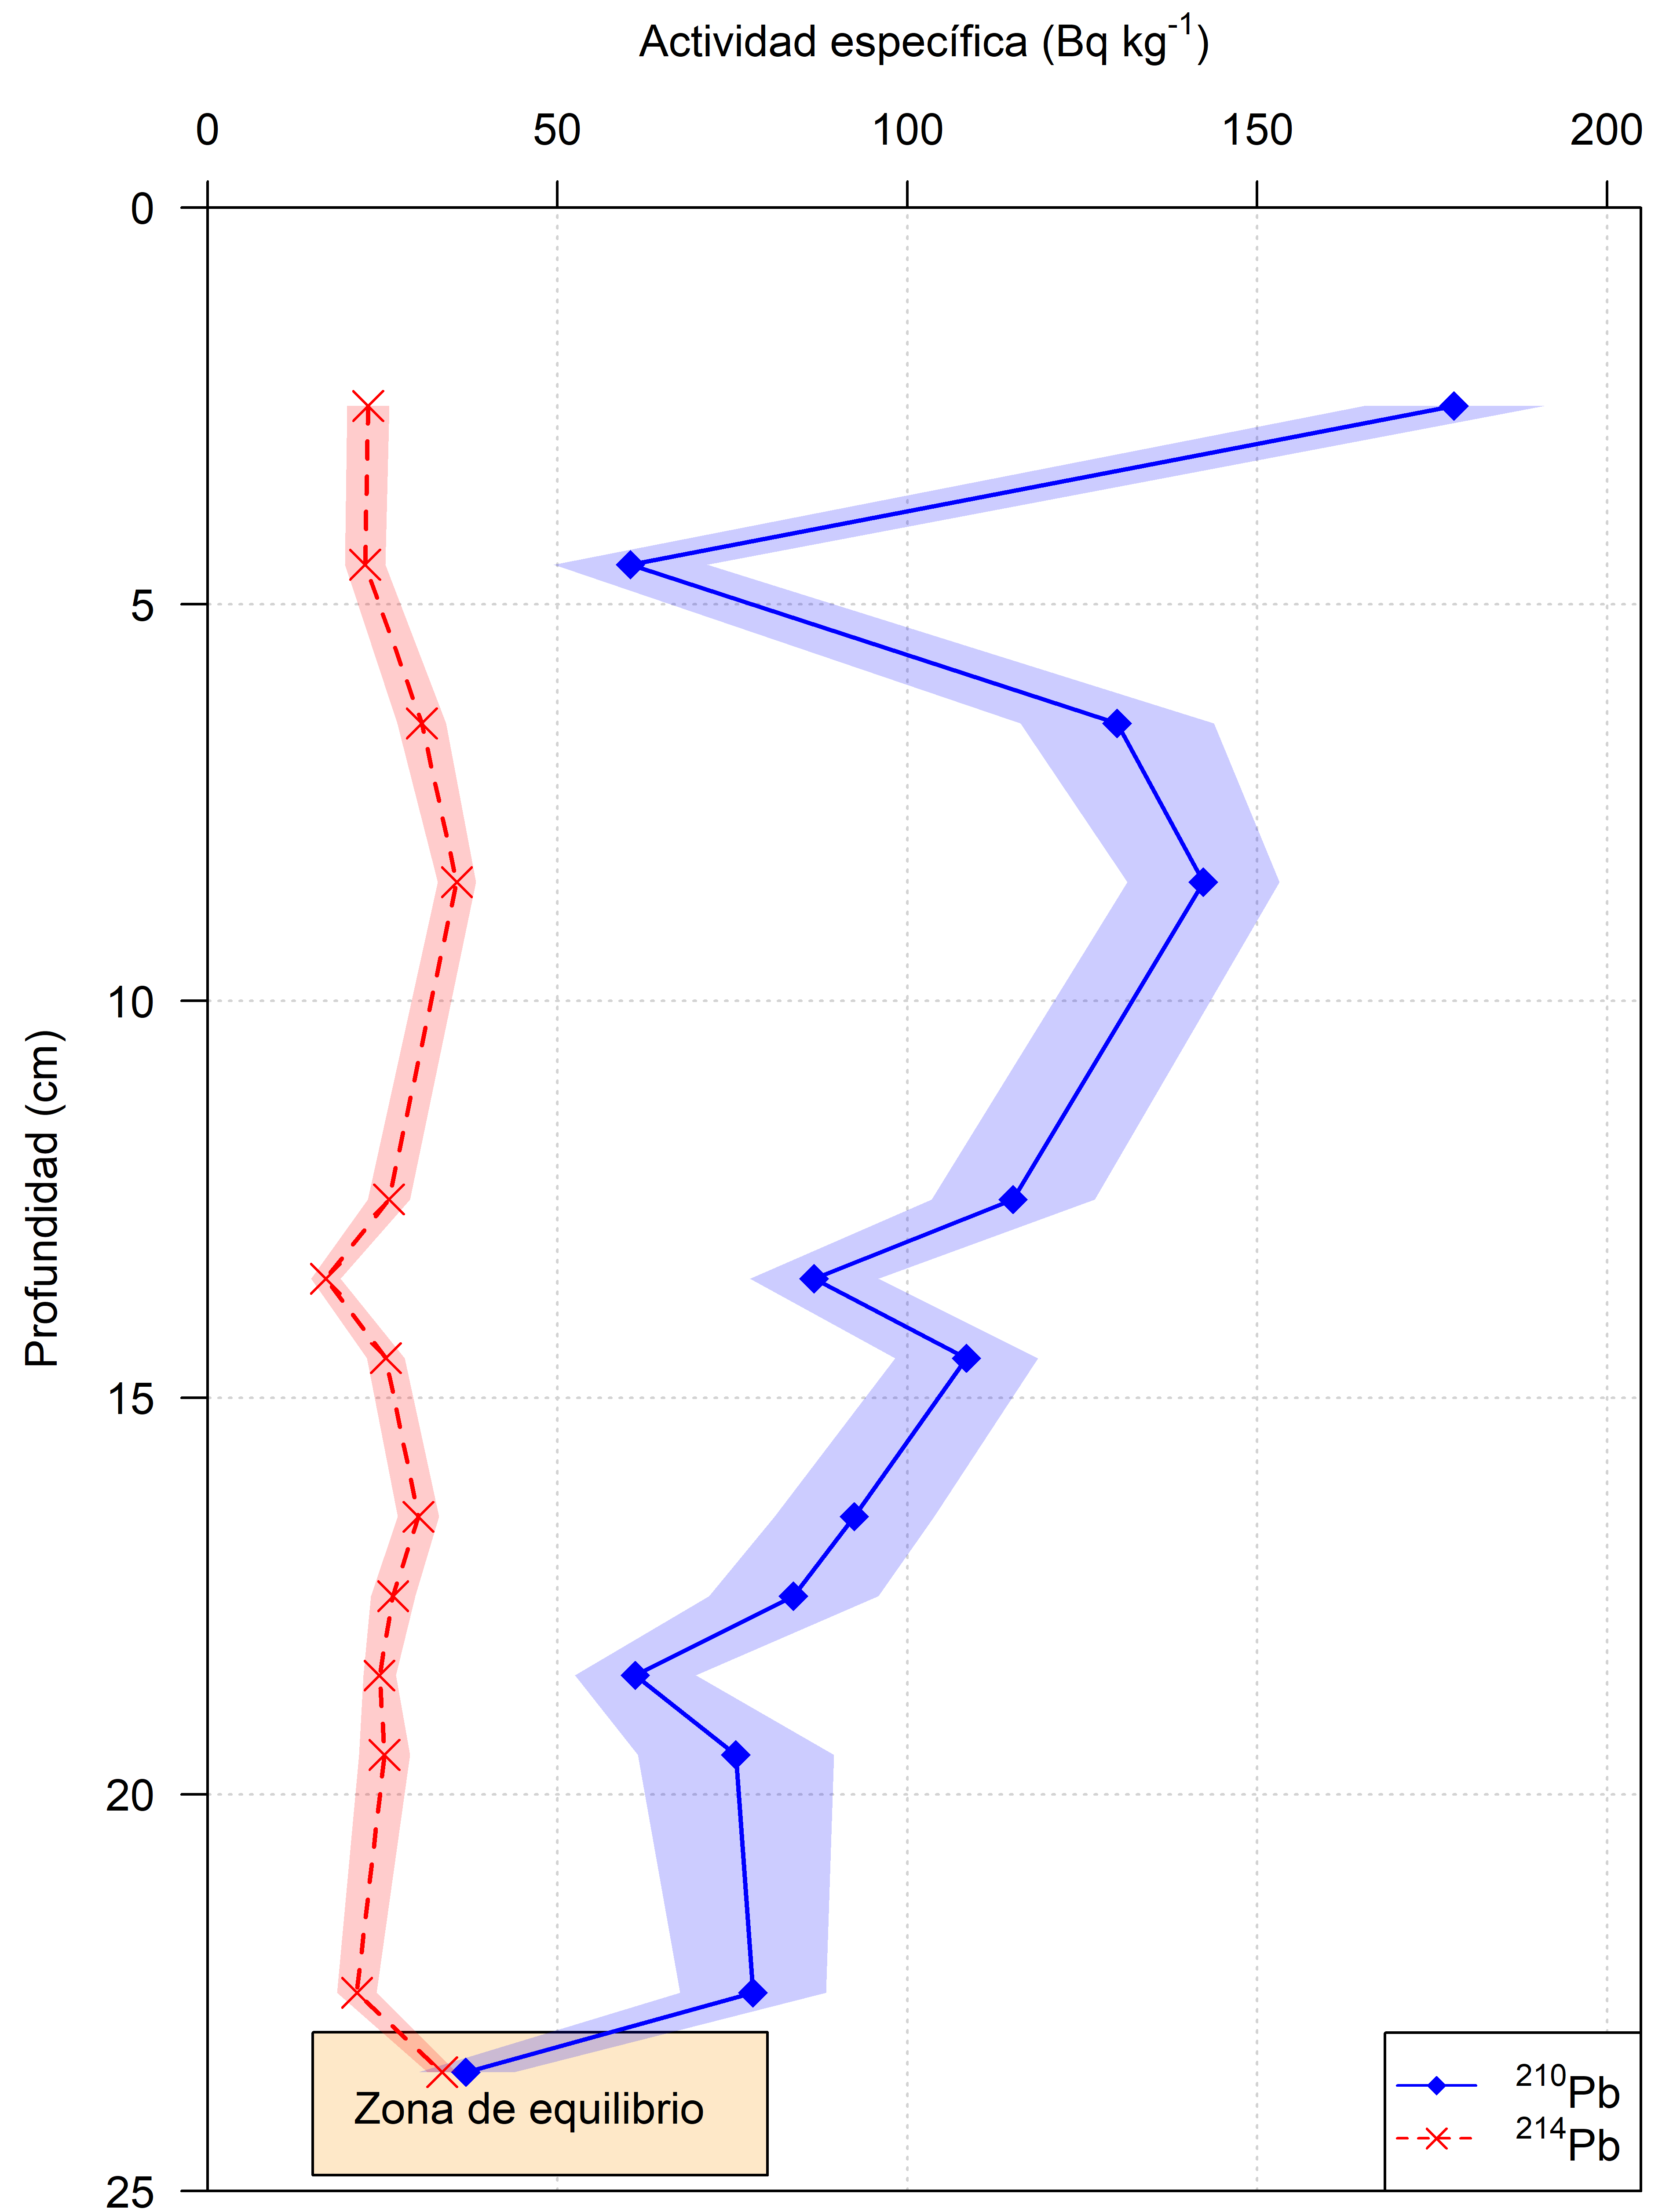
\includegraphics[width=0.9\textwidth]{Imagenes/Act_210Pb_214Pb_SAMO-14-2.png}
\caption{Perfiles de actividad específica de \PbCero\, y \PbCuatro\,corregidos para el núcleo sedimentario \textbf{SAMO-14-2}. La última sección posiblemente se encuentra en equilibrio secular.}\label{Fig-SAMO142-Comp}
\end{figure}
\begin{figure}
\centering
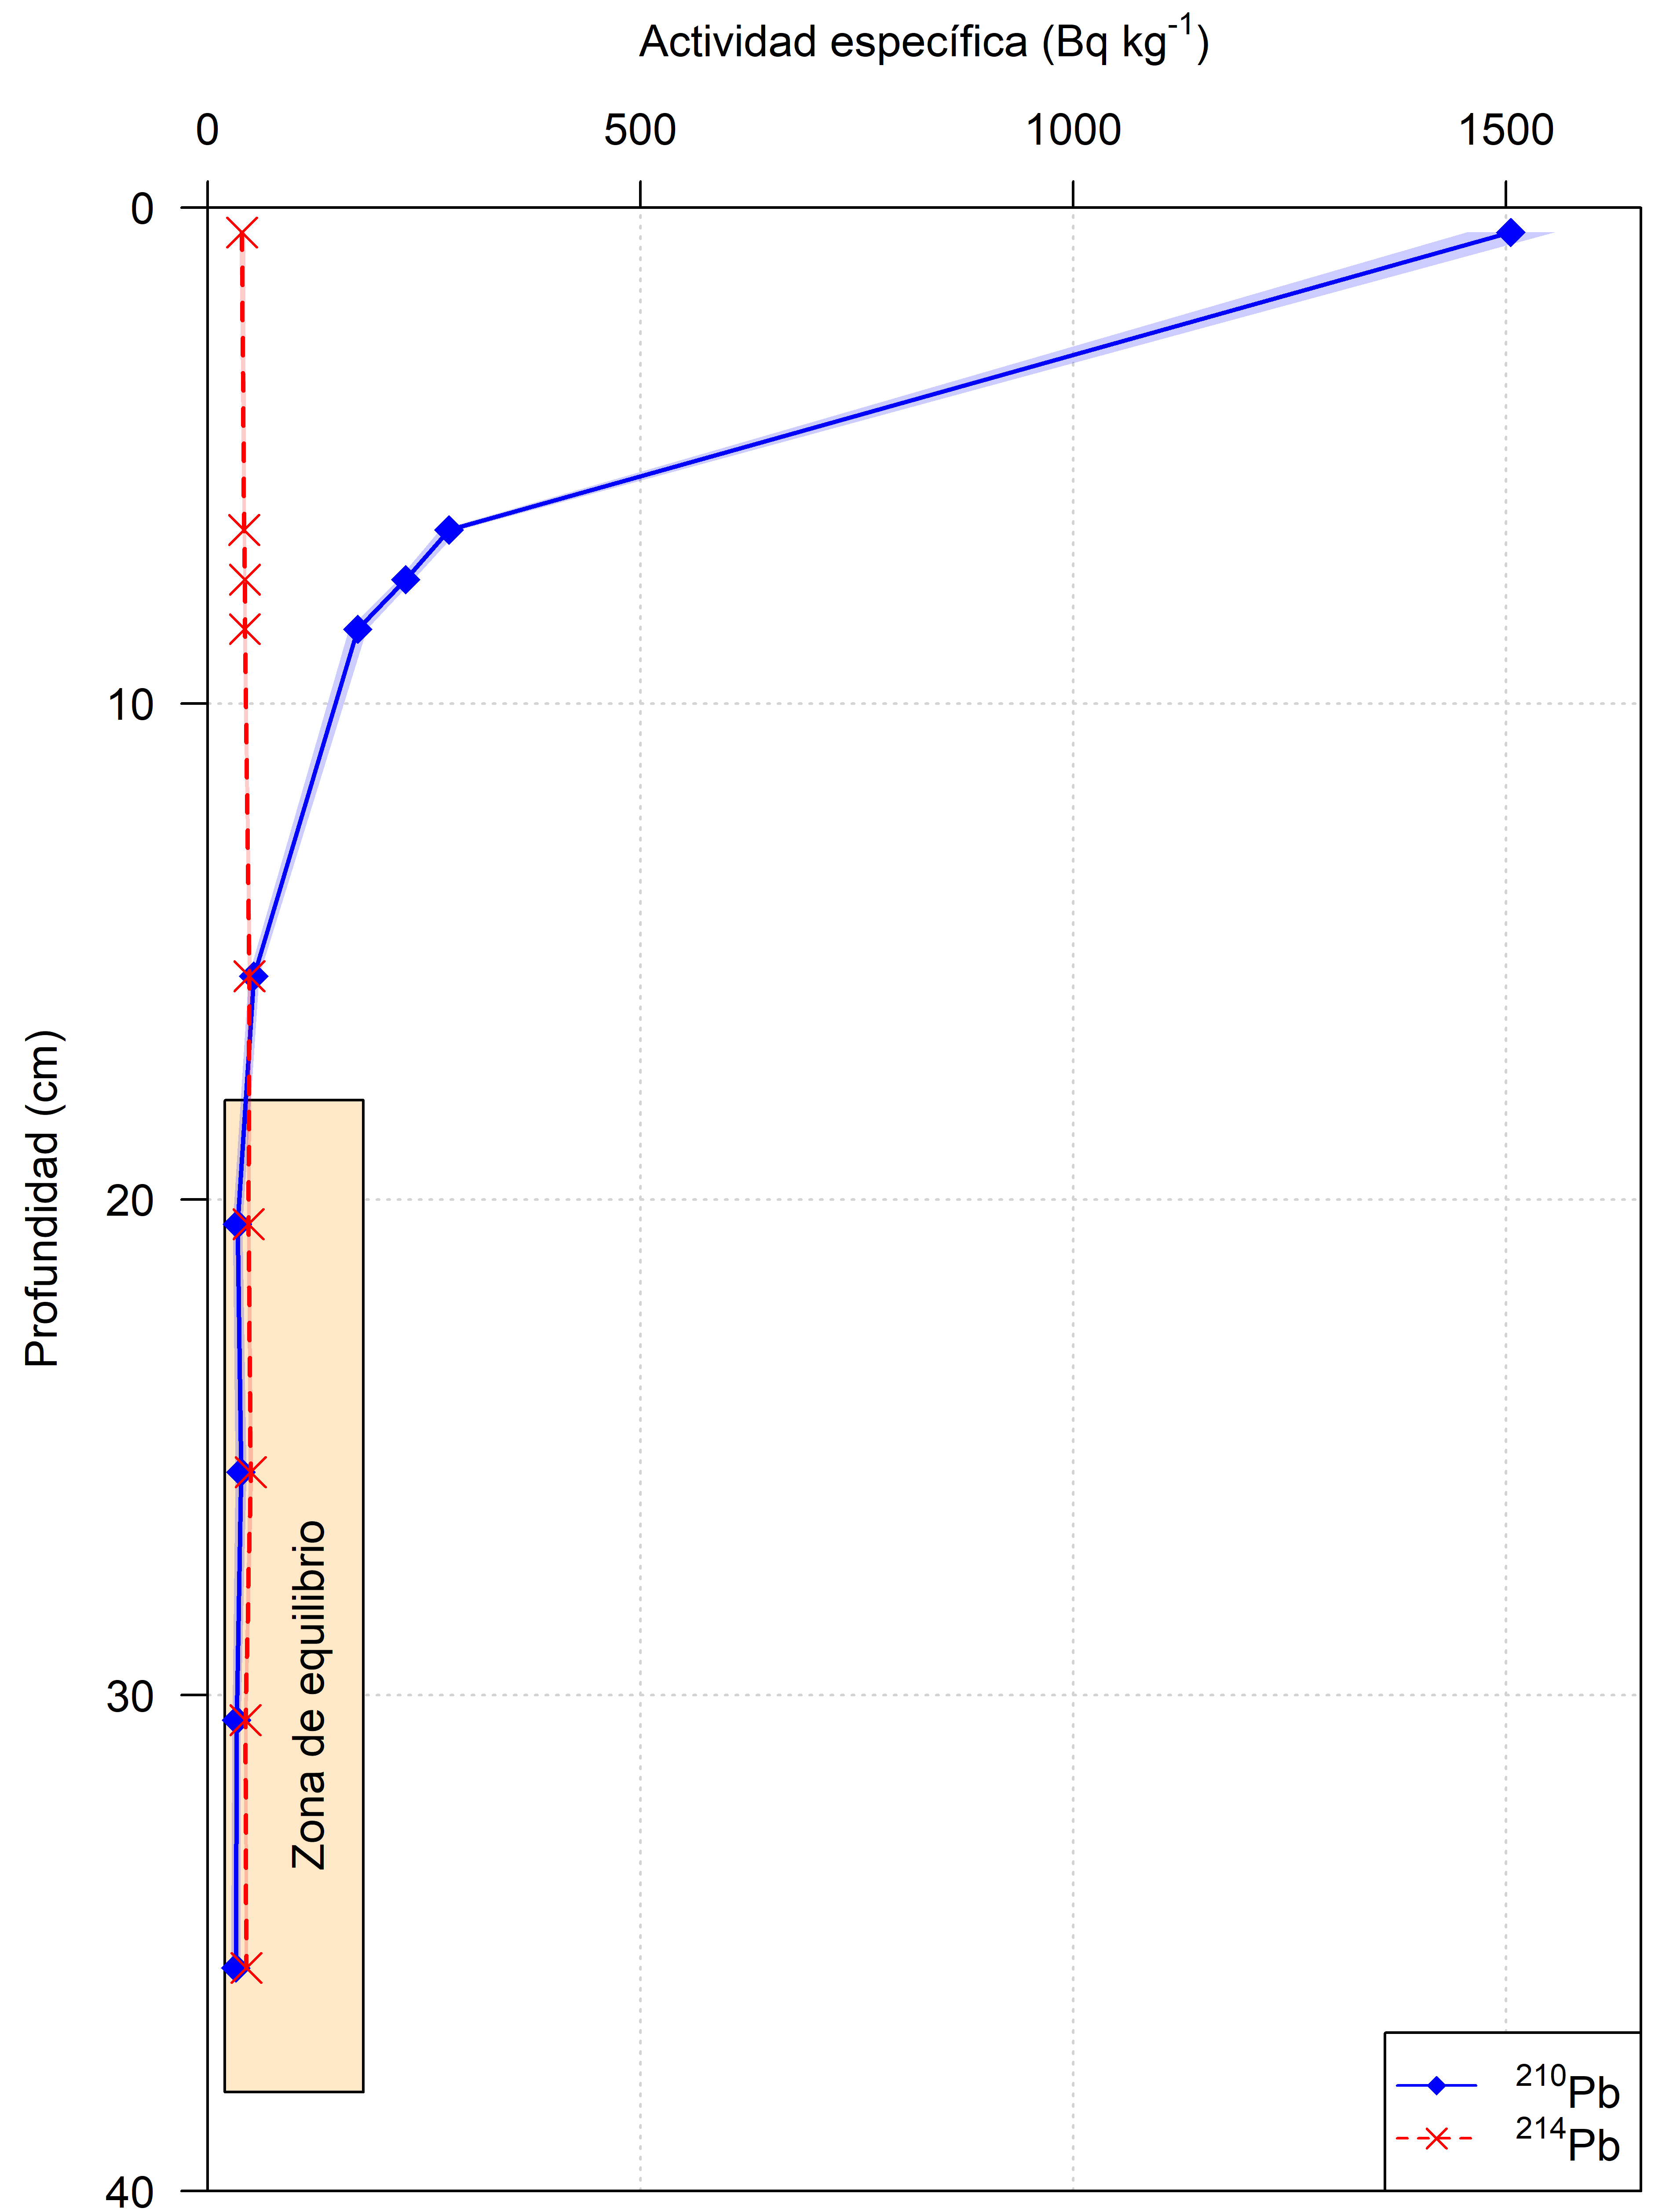
\includegraphics[width=0.9\textwidth]{Imagenes/Act_210Pb_214Pb_TEHUA-XII.png}
\caption{Perfiles de actividad específica de \PbCero\, y \PbCuatro\,corregidos para el núcleo sedimentario \textbf{TEHUA-XII}. Las cuatro últimas secciones posiblemente se encuentran en equilibrio secular.}\label{Fig-TEHUAXII-Comp}
\end{figure}
\begin{figure}
\centering
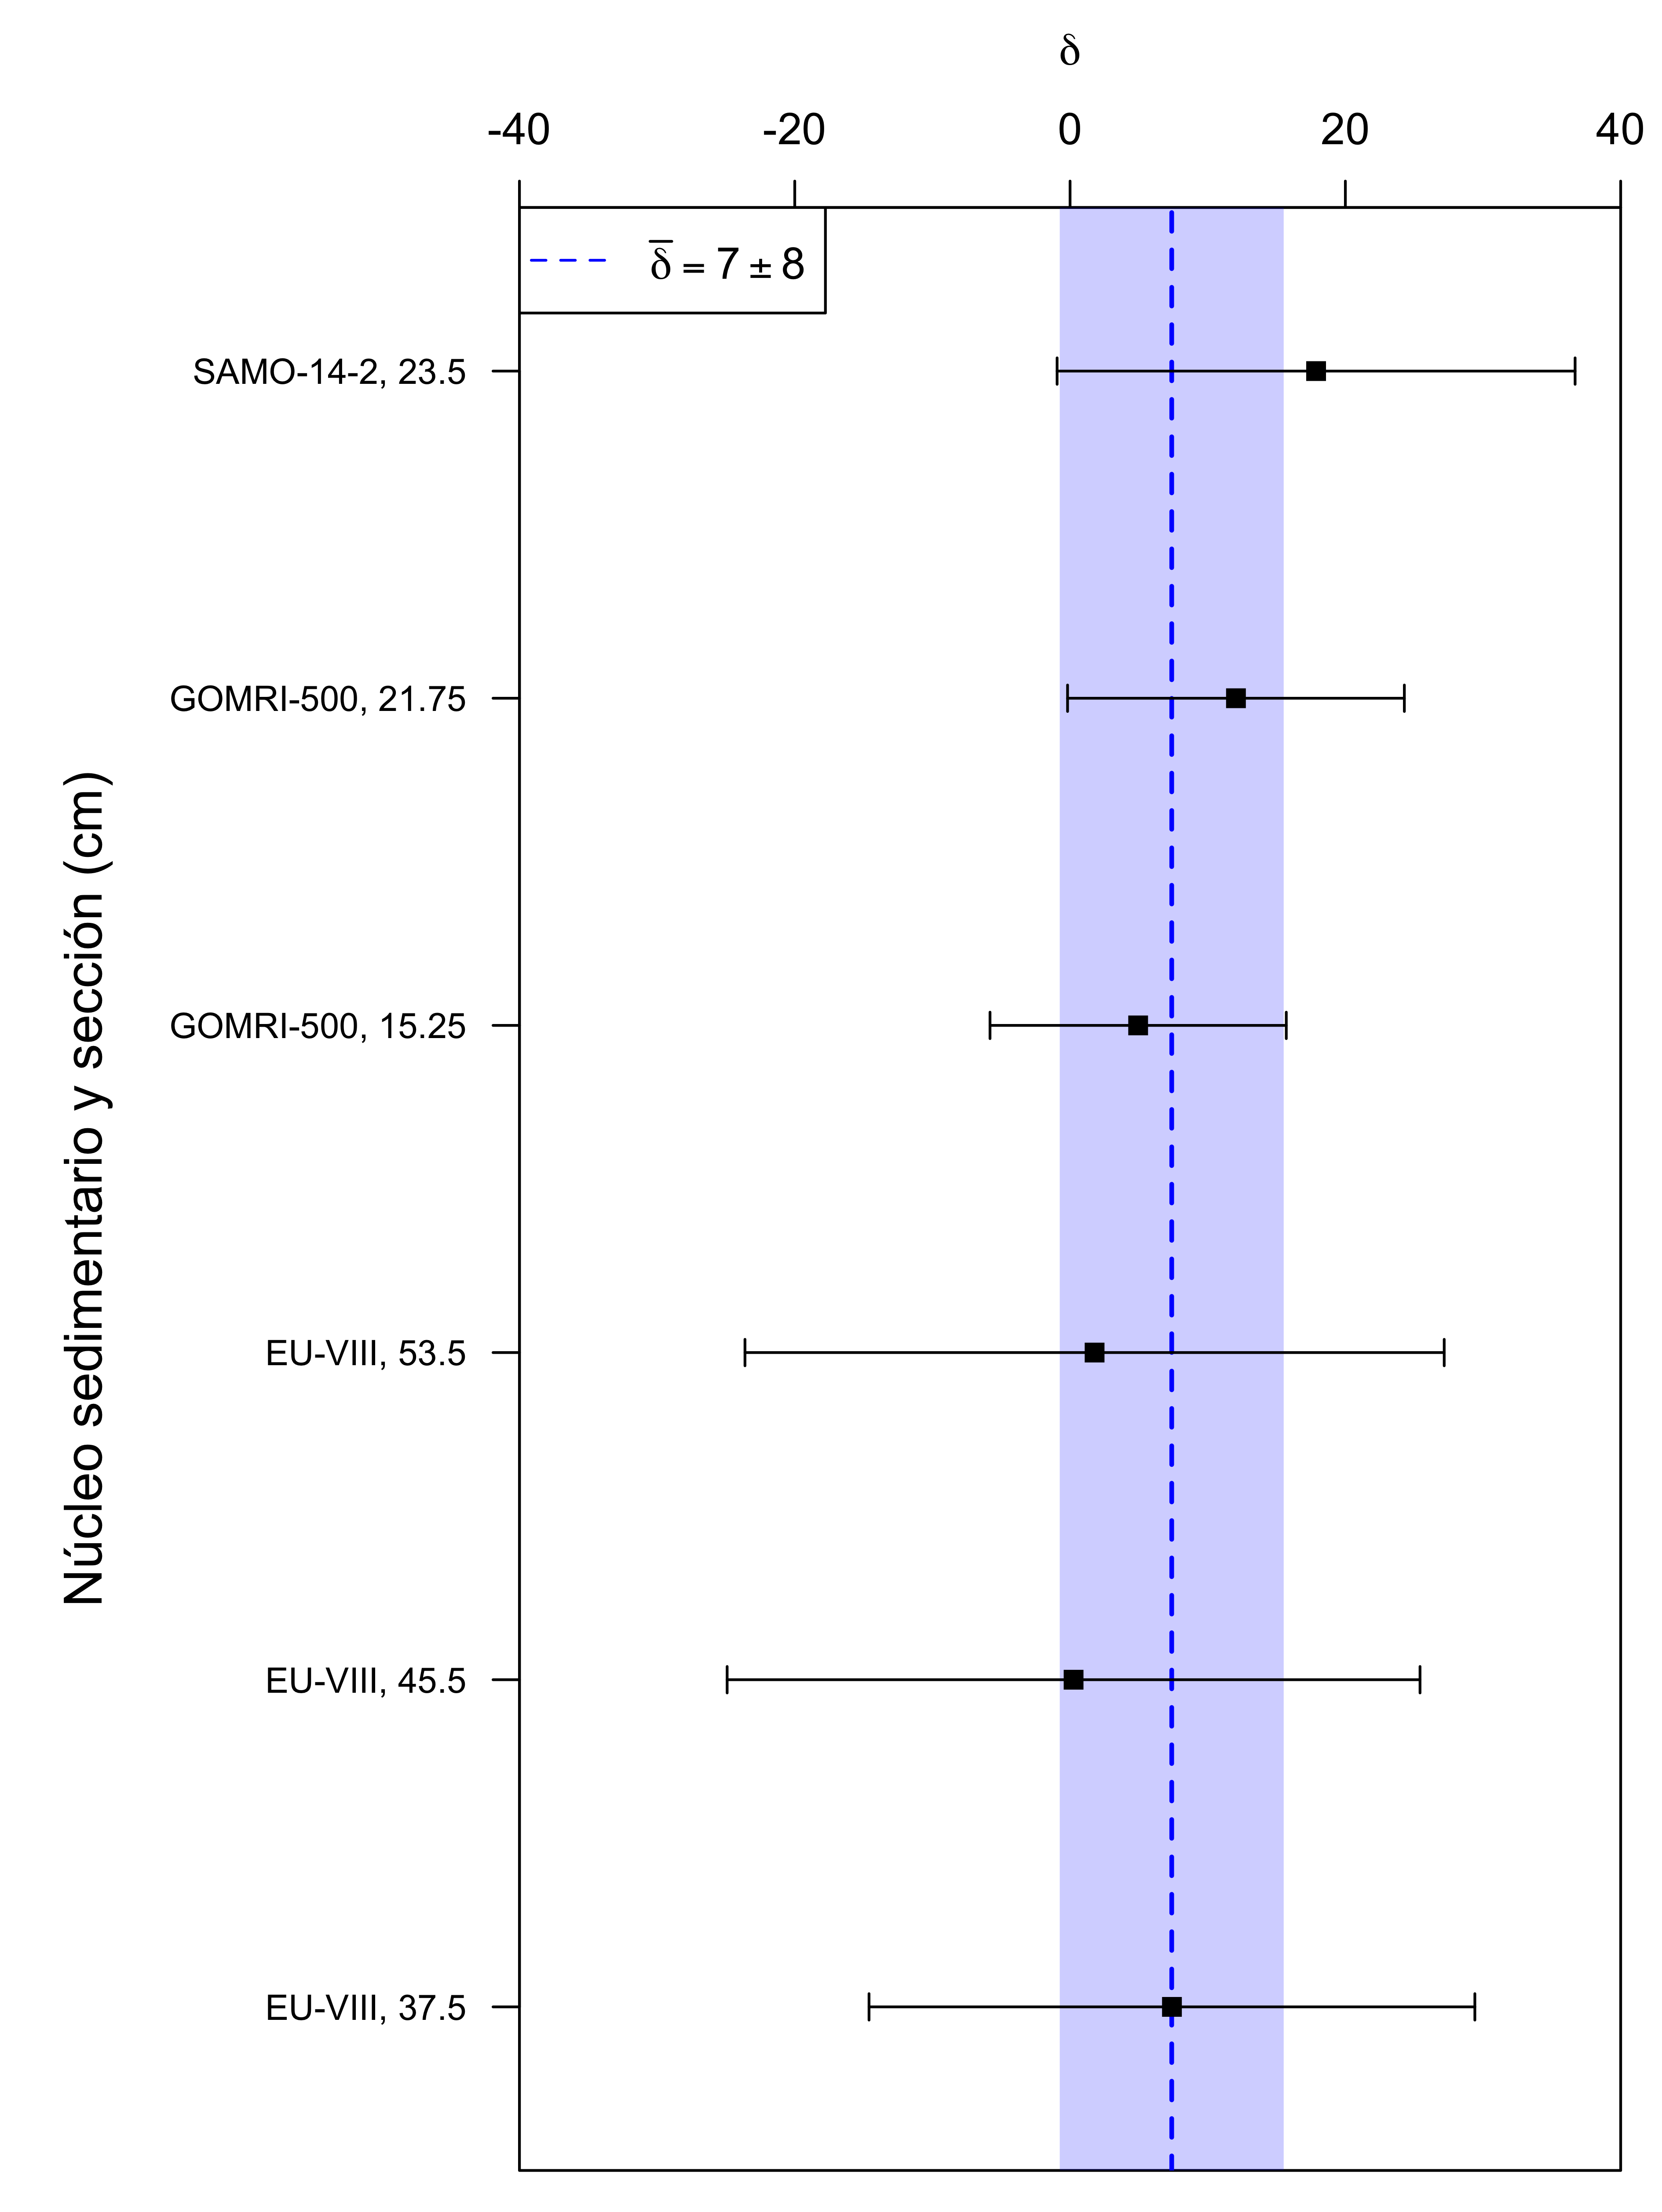
\includegraphics[width=0.9\textwidth]{Imagenes/Grafica_Delta_210Pb_214Pb-2.png}
\caption{Diferencia porcentual $\delta$ de los valores de la actividad específica de \PbCero\, respecto a la actividad específica de \PbCuatro\, para las secciones que se encuentran en equilibrio de los núcleos sedimentarios EU-VIII, GOMRI-500 y SAMO-14-2 asumiendo una composición corregida.}\label{Fig-DiffPorcentualEquilibrio}
\end{figure}
\newpage
	\section{Fechado}\label{Seccion-Fechado}
Las actividades de referencia y corregidas, y las profundidades a partir de las cuales se asumió el equilibrio secular, fueron utilizadas para establecer los modelos de edad con el modelo CF (Sección \ref{SubSec-Fechado}). En todos los casos, y como es conocido \cite{SANCHEZCABEZA2012183}, las incertidumbres de los modelos de edad crecen con la profundidad. Los modelos de edad y las diferencias porcentuales para los núcleos sedimentarios con composición corregida y composición no corregida se muestran en las Figuras \ref{ModeloEdad-EUVIII}, \ref{ModeloEdad-GOMRI500}, \ref{ModeloEdad-PCm}, \ref{ModeloEdad-LTAF}, \ref{ModeloEdad-SAMO} y \ref{ModeloEdad-TEHUAXII}, y los promedios de las diferencias porcentuales en la Tabla \ref{Tabla-DiferenciasPorcentualesFechado}. 
\\
\\
La Tabla \ref{Tabla-DiferenciasPorcentualesFechado} muestra la variabilidad de las diferencias porcentuales promedios de las eficiencias y de las masas, así como las diferencias porcentuales promedio en los modelos de edad. 
\\
\\
De acuerdo con la mínima corrección en eficiencia realizada, el núcleo PCm mostró modelos de edad prácticamente coincidentes con una diferencia porcentual entre los modelos de 0.1 \% (Figura \ref{ModeloEdad-PCm}, Tabla \ref{Tabla-DiferenciasPorcentualesFechado}). En el otro extremo, si bien la mayor corrección promedio fue para el núcleo GOMRI-500, su desviación promedio en el modelo de edad fue de las más bajas (3 $\pm$ 2 \%). En esta misma dirección, la corrección del modelo de edad más fuerte fue para el núcleo EU-VIII (22 $\pm$ 2 \%), que sí mostró una corrección de eficiencia importante (12 \%). Es pues claro que la corrección de eficiencia no es la única variable que explica la variación en los modelos de edad. 
\\
\\
Por otra parte, en el modelo de fechado de Flujo Constante, el fechado corregido $t$ de una sección es 
\begin{equation}
t(i) =  \dfrac{1}{\lambda}\,\ln\left(\dfrac{\sum_{j=1}^\infty A_{j, \text{corr}}\, m_j}{ \sum_{j=i+1}^\infty A_{j, \text{corr}}\, m_j}\right) = 
\dfrac{1}{\lambda}\,\ln\left(\dfrac{\sum_{j=1}^\infty \dfrac{\epsilon_{j, \text{ref}}}{\epsilon_{j, \text{corr}}} A_{j, \text{ref}}\, m_j}{ \sum_{j=i+1}^\infty \dfrac{\epsilon_{j, \text{ref}}}{\epsilon_{j, \text{corr}}} A_{j, \text{ref}}\, m_j}\right).
\end{equation}
Si las eficiencias de referencia $\epsilon_{j, \text{ref}}$ y corregida $\epsilon_{j, \text{corr}}$ de la sección $j$ son constantes a lo largo del núcleo, entonces $A_{j, \text{corr}} \propto A_{j, \text{ref}}$ para todo valor de $j$ (Ecuación \ref{Eq-ActividadCorregida}) y el fechado $t$ no se ve afectado.
\\
\\
Por lo tanto, es posible que las diferencias en los modelos de edad no se deban tanto a la corrección de eficiencia sino a su variabilidad (es decir, que no se cumpla la hipótesis de una corrección de eficiencia constante). Como se observa en la Tabla \ref{Tabla-DiferenciasPorcentualesFechado}, la variabilidad de la corrección de eficiencia también influye en la corrección del fechado, pero no es la única variable relevante. El fechado con el modelo CF también requiere el conocimiento de las masas, que presentan una fuerte variabilidad como se observa en la Tabla \ref{Tabla-DiferenciasPorcentualesFechado}. Por lo tanto, es la combinación compleja de los valores absolutos y variabilidades de las masas y las eficiencias las que determinan la desviación final del modelo de edad corregido y, por ello, dependerá de cada caso concreto. Esta conclusión acentúa la necesidad de disponer de actividades absolutas lo más próximas a las reales y una medida confiable de la masa real de cada sección.
\begin{figure}[h]
\centering
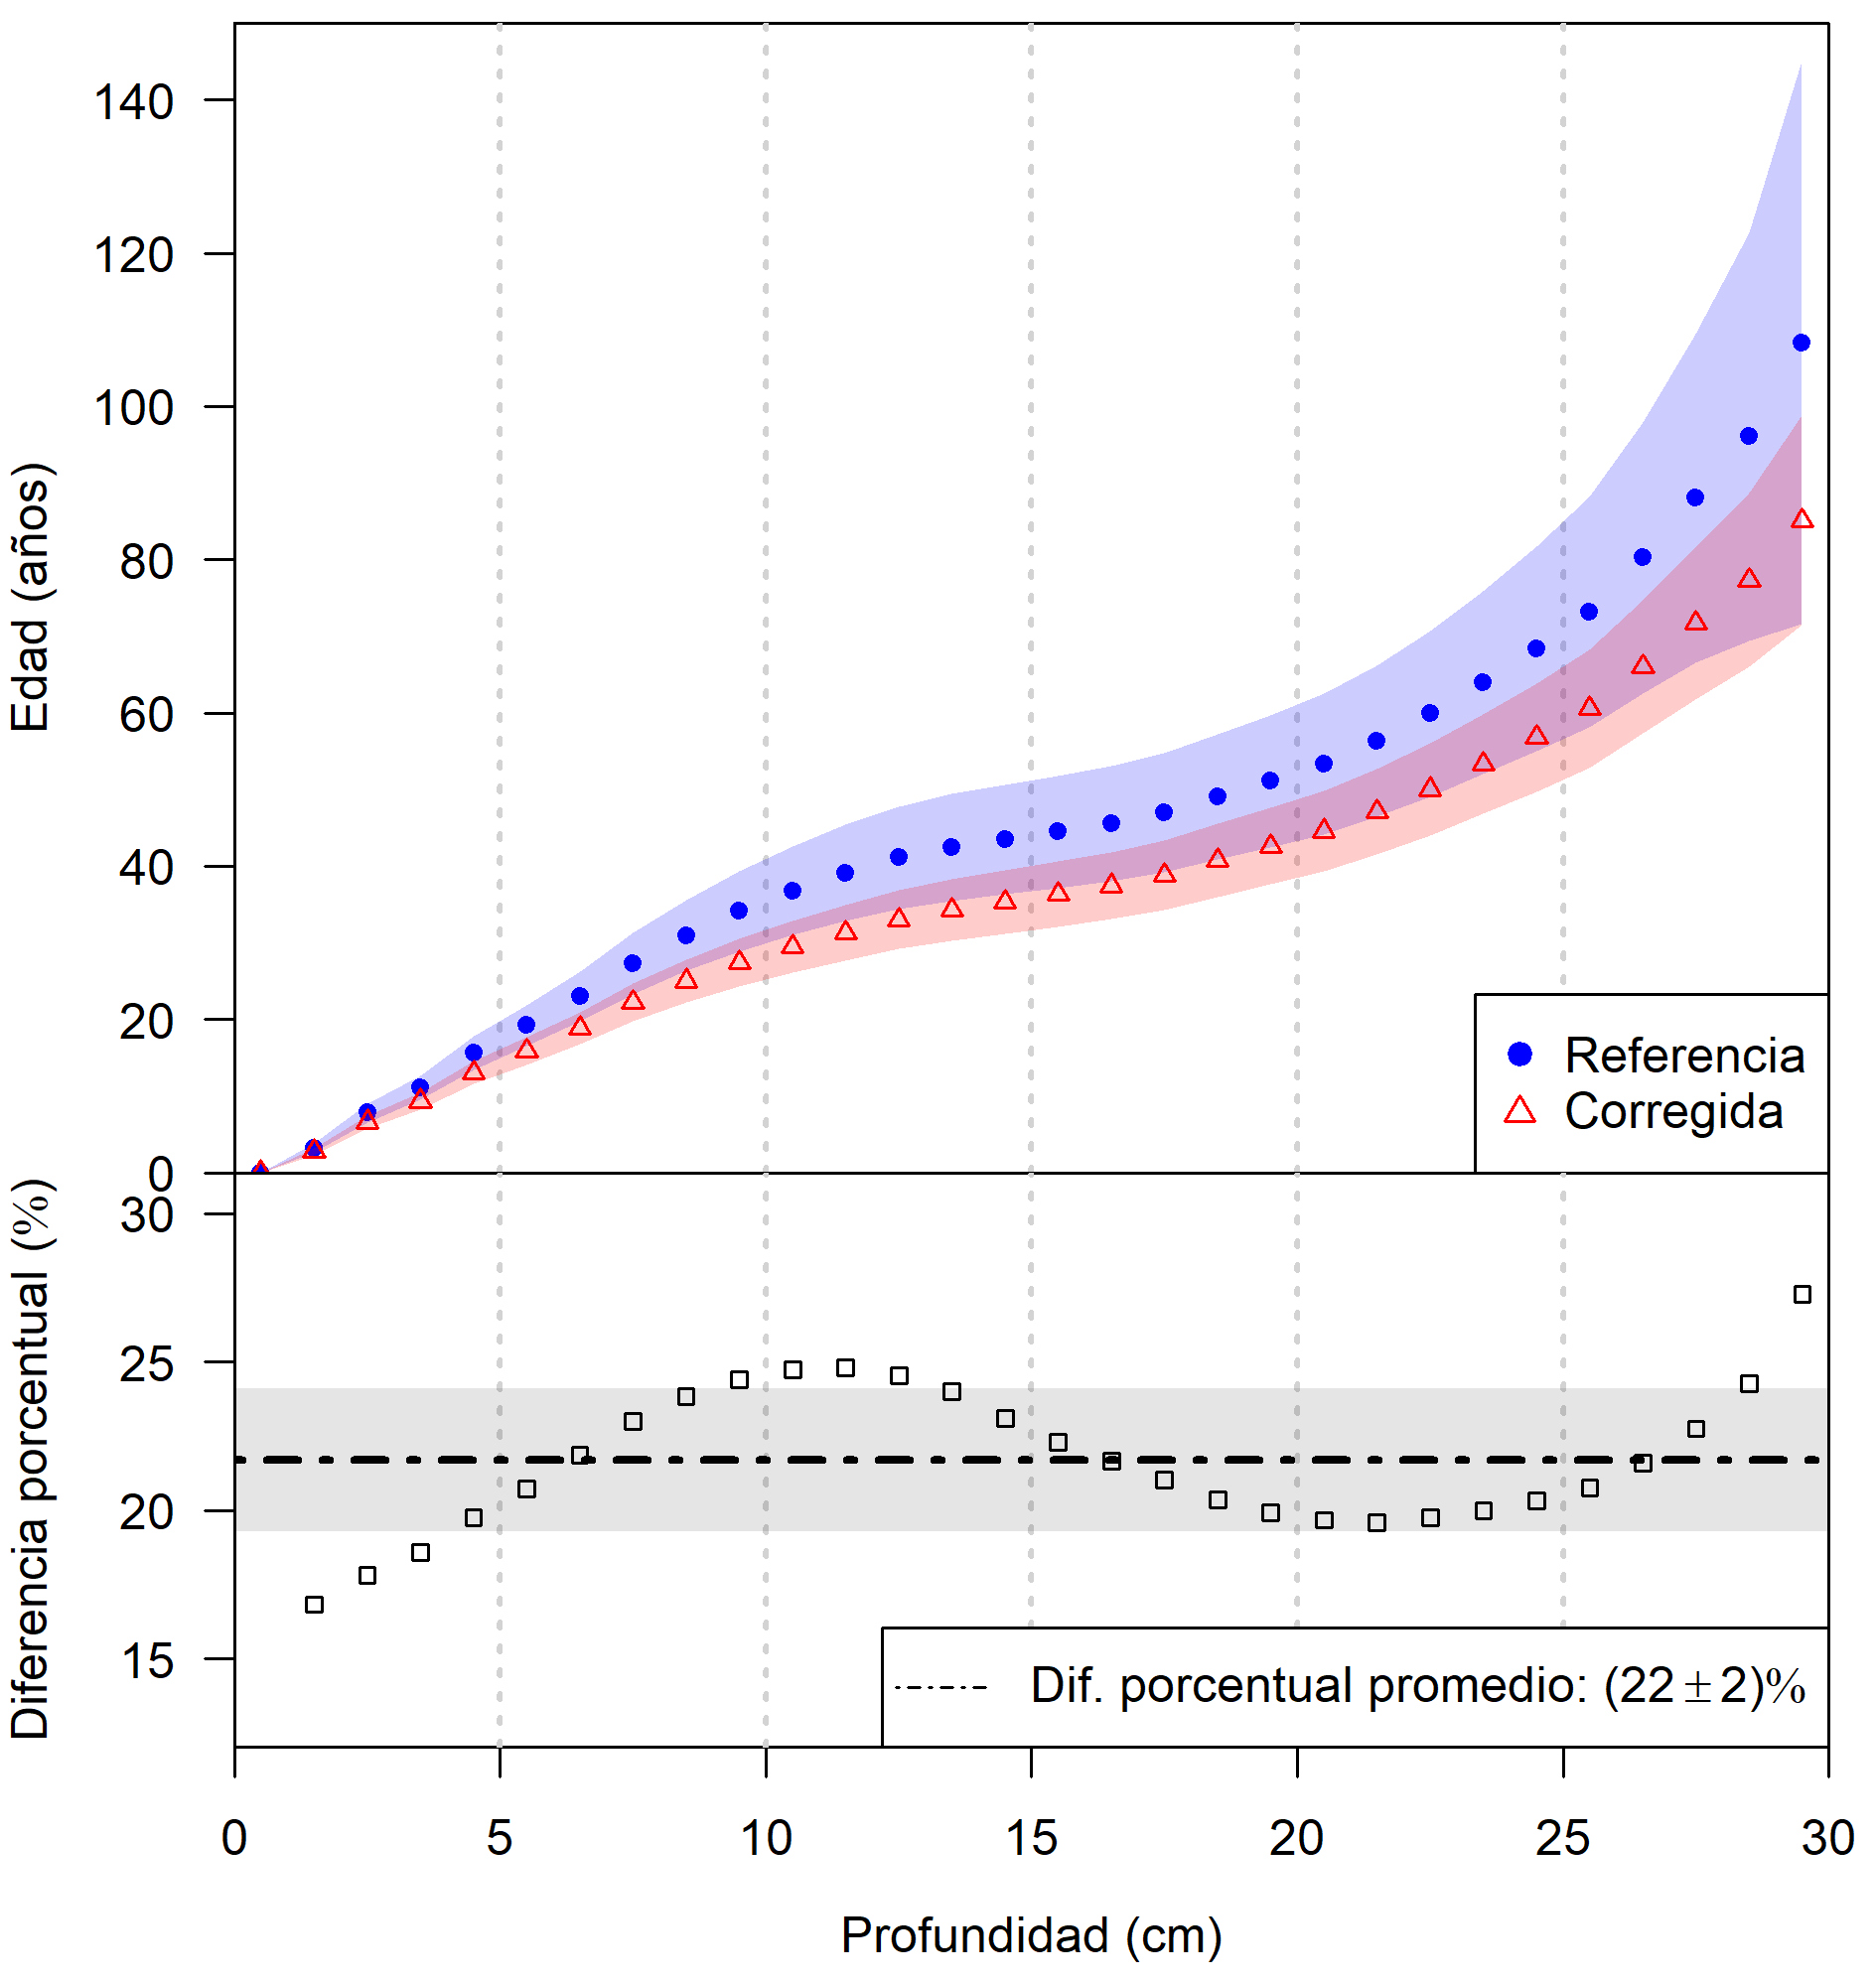
\includegraphics[width=0.9\textwidth]{Imagenes/EUVIII_1.png}
\caption{Modelo de edad del núcleo \textbf{EU-VIII} para la composición de referencia y la composición corregida. En la parte inferior se muestra la diferencia porcentual respecto a composición de referencia.}\label{ModeloEdad-EUVIII}
\end{figure}

\begin{figure}[h]
\centering
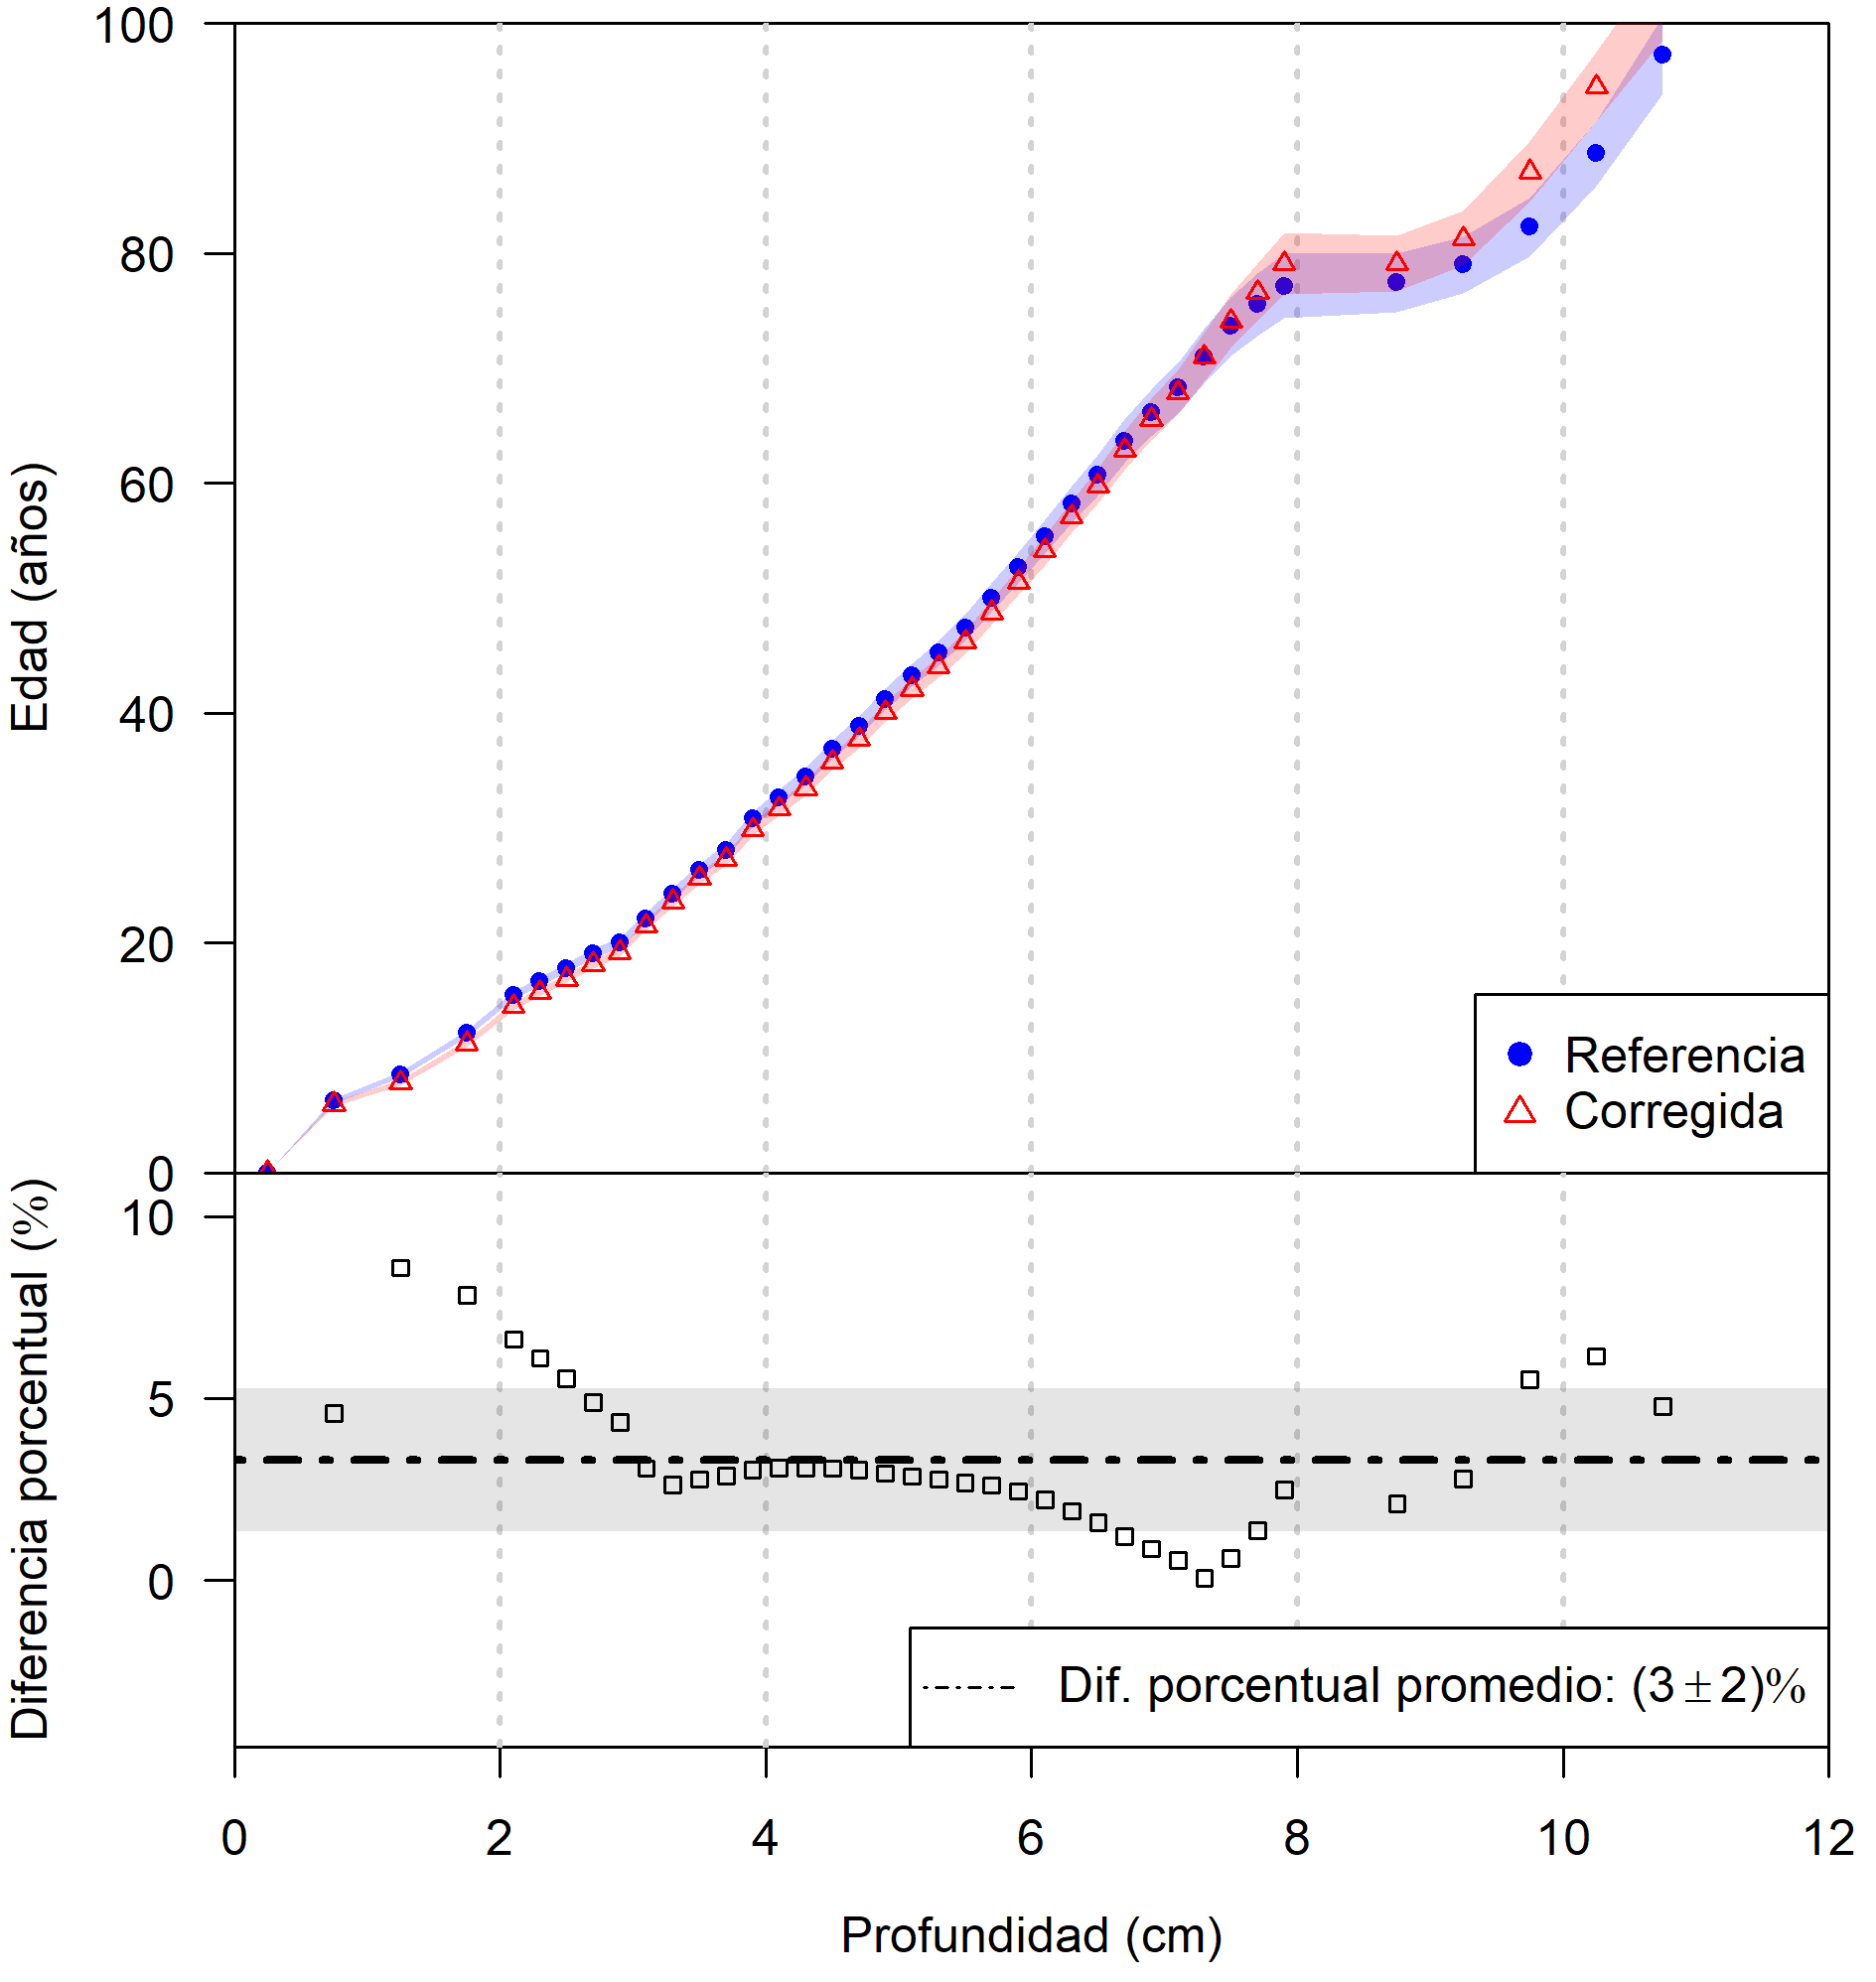
\includegraphics[width=0.9\textwidth]{Imagenes/GOMRI500_1.png}
\caption{Modelo de edad del núcleo \textbf{GOMRI-500} para la composición de referencia y la composición corregida. En la parte inferior se muestra la diferencia porcentual respecto a composición de referencia.}\label{ModeloEdad-GOMRI500}
\end{figure}

\begin{figure}[h]
\centering
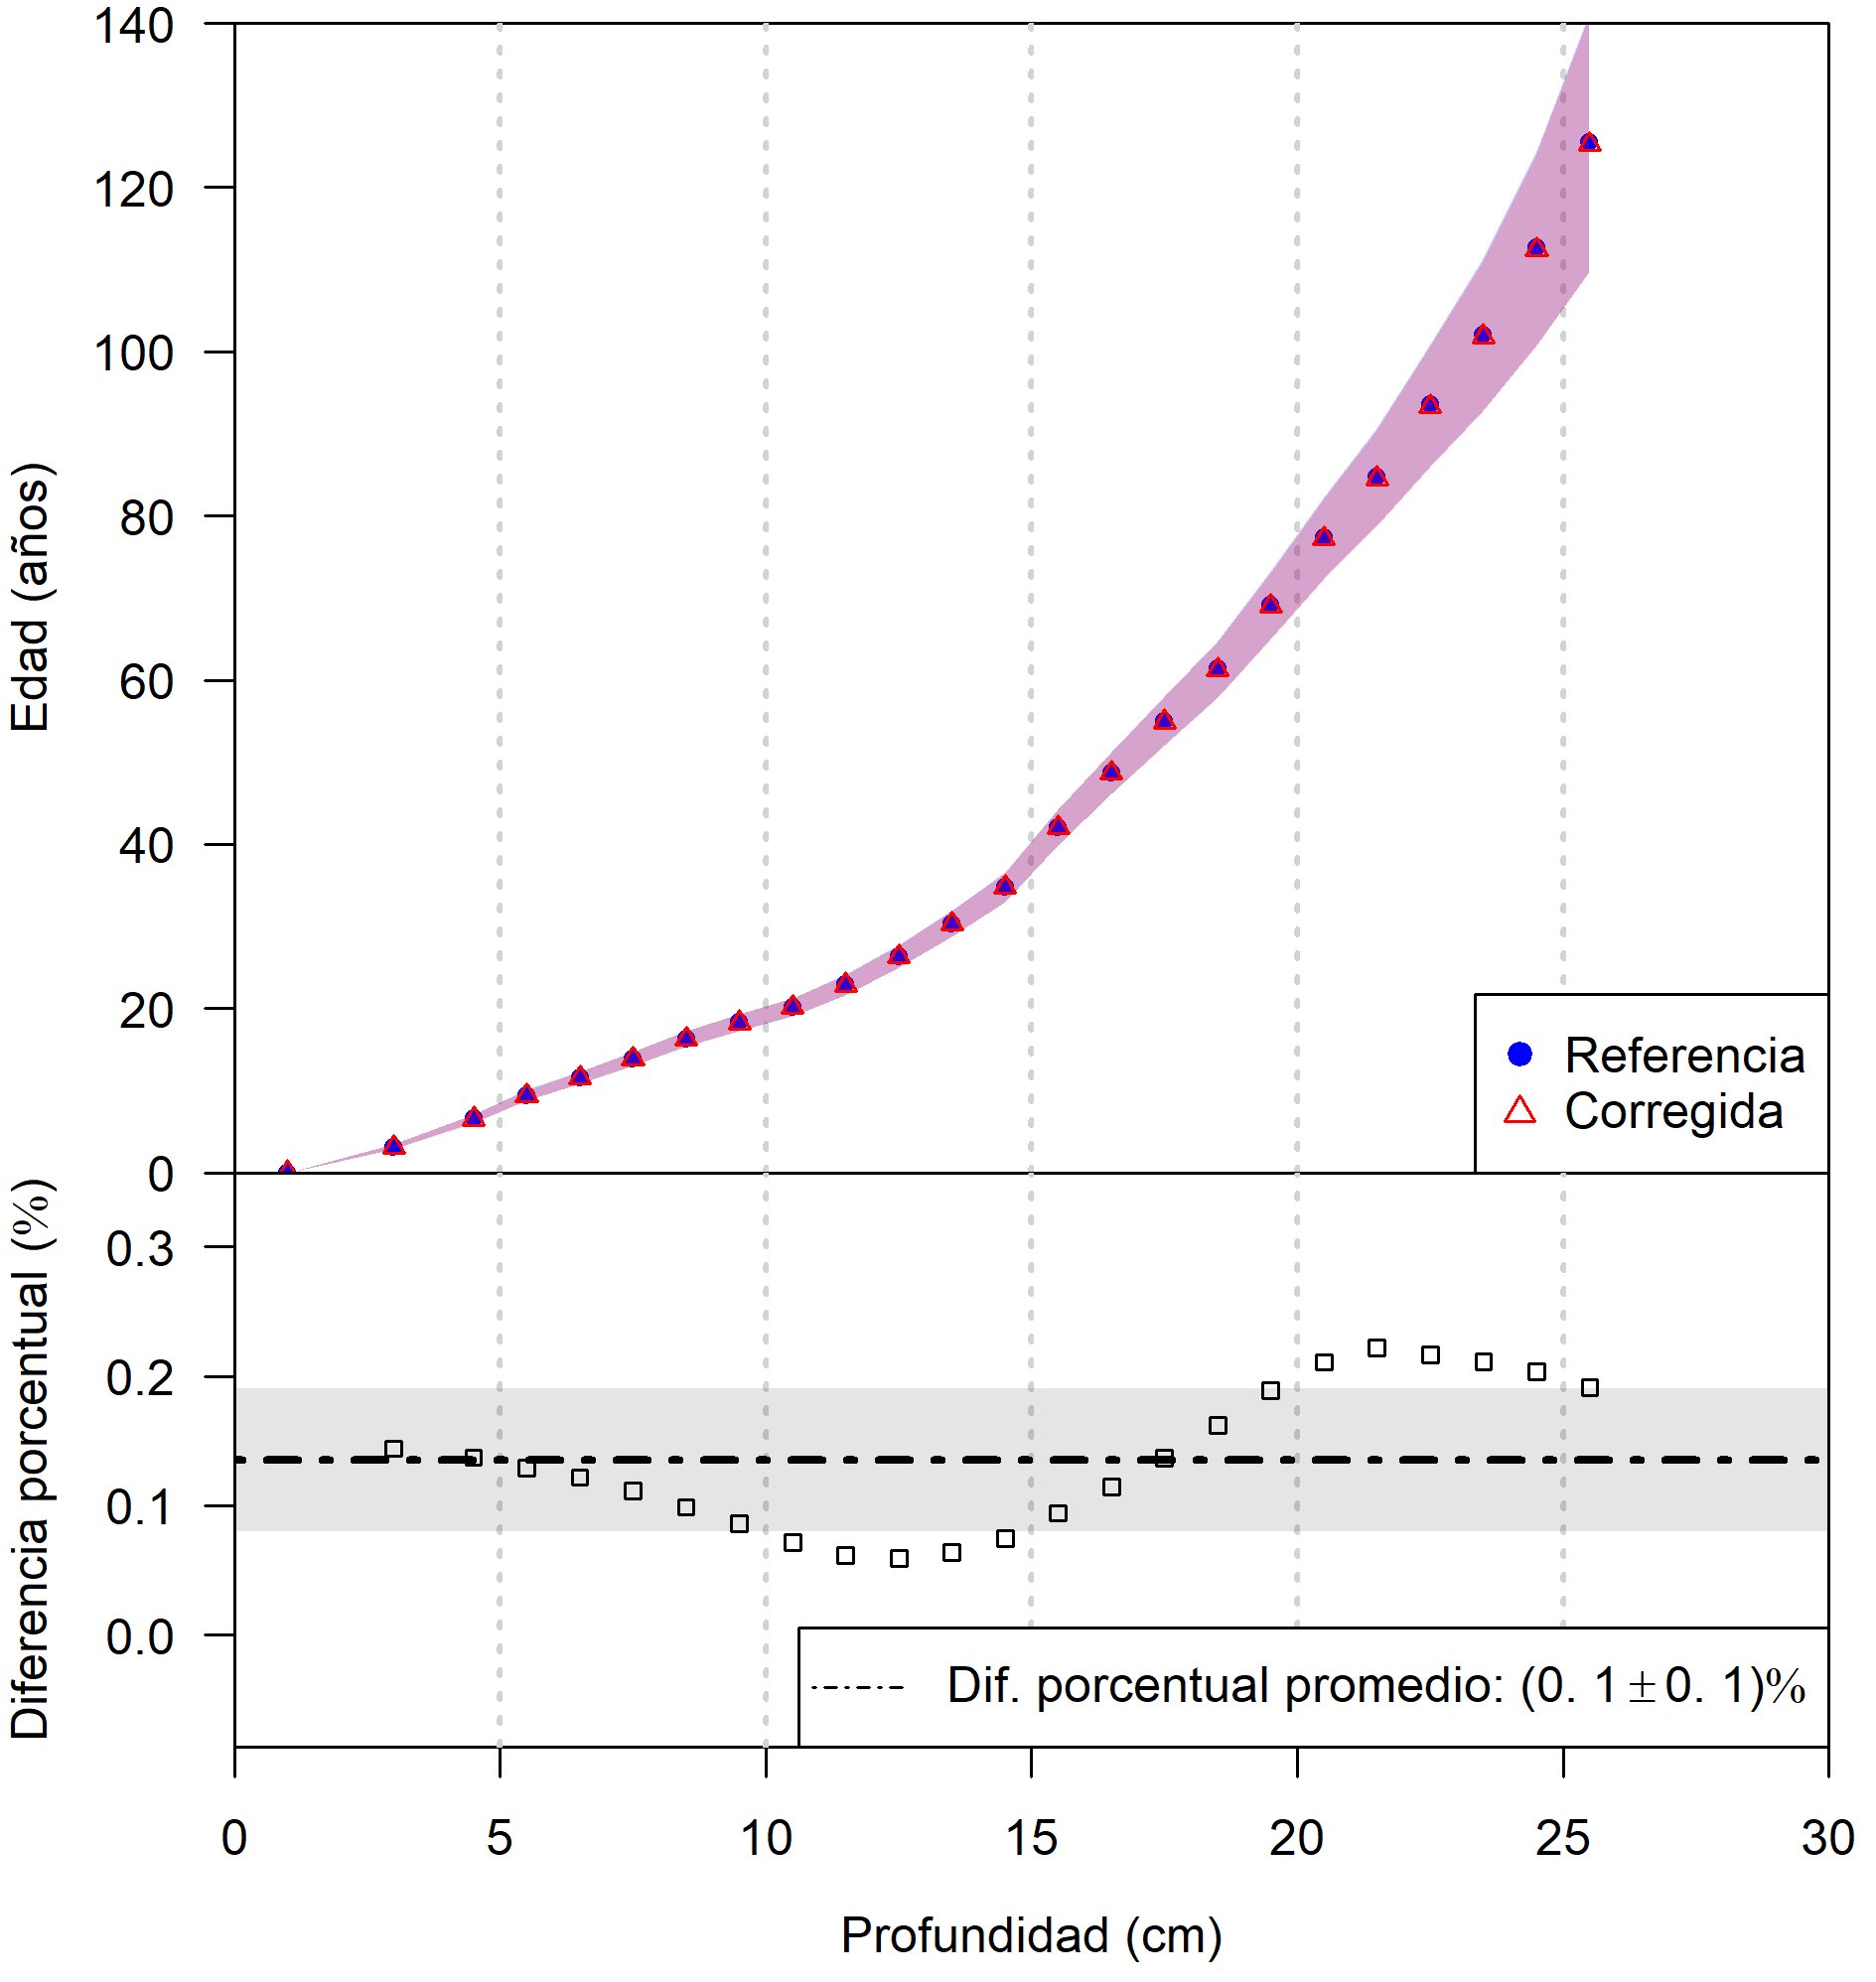
\includegraphics[width=0.9\textwidth]{Imagenes/PCm_1.png}
\caption{Modelo de edad del núcleo \textbf{PCm} para la composición de referencia y la composición corregida. En la parte inferior se muestra la diferencia porcentual respecto a composición de referencia.}\label{ModeloEdad-PCm}
\end{figure}

\begin{figure}[h]
\centering
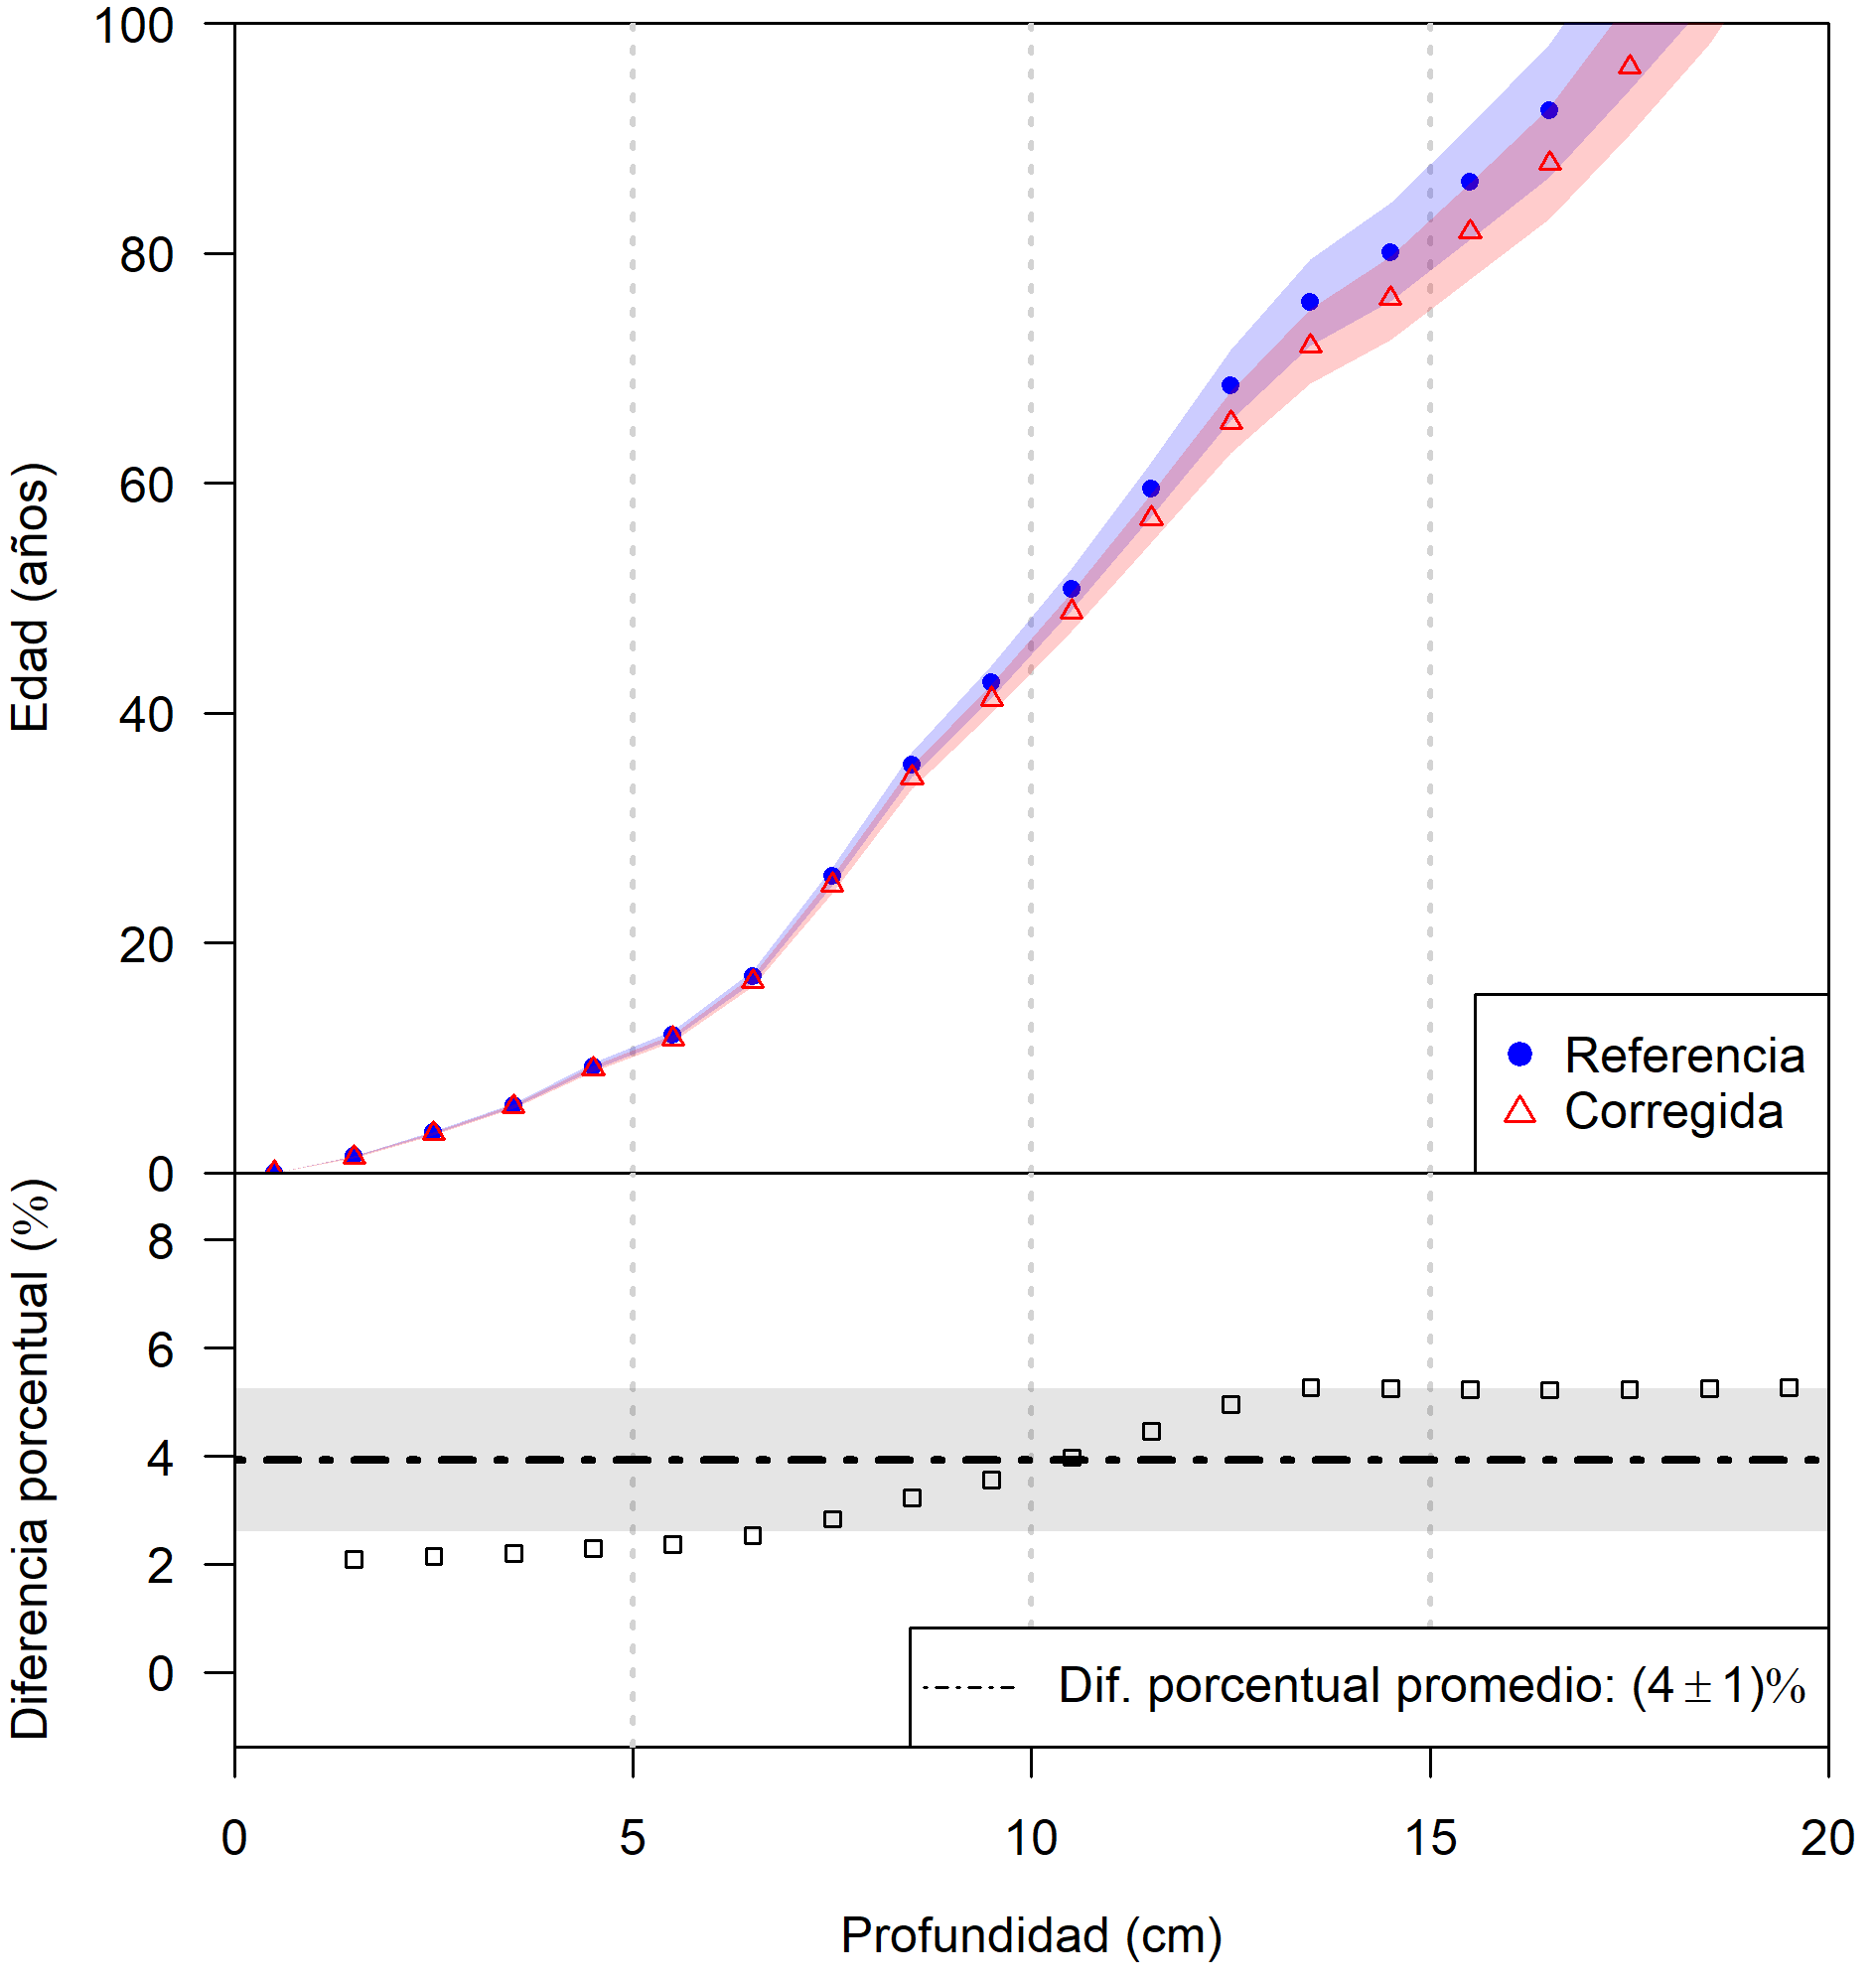
\includegraphics[width=0.9\textwidth]{Imagenes/LTAF_1.png}
\caption{Modelo de edad del núcleo \textbf{LTAF} para la composición de referencia y la composición corregida. En la parte inferior se muestra la diferencia porcentual respecto a composición de referencia.}\label{ModeloEdad-LTAF}
\end{figure}

\begin{figure}[h]
\centering
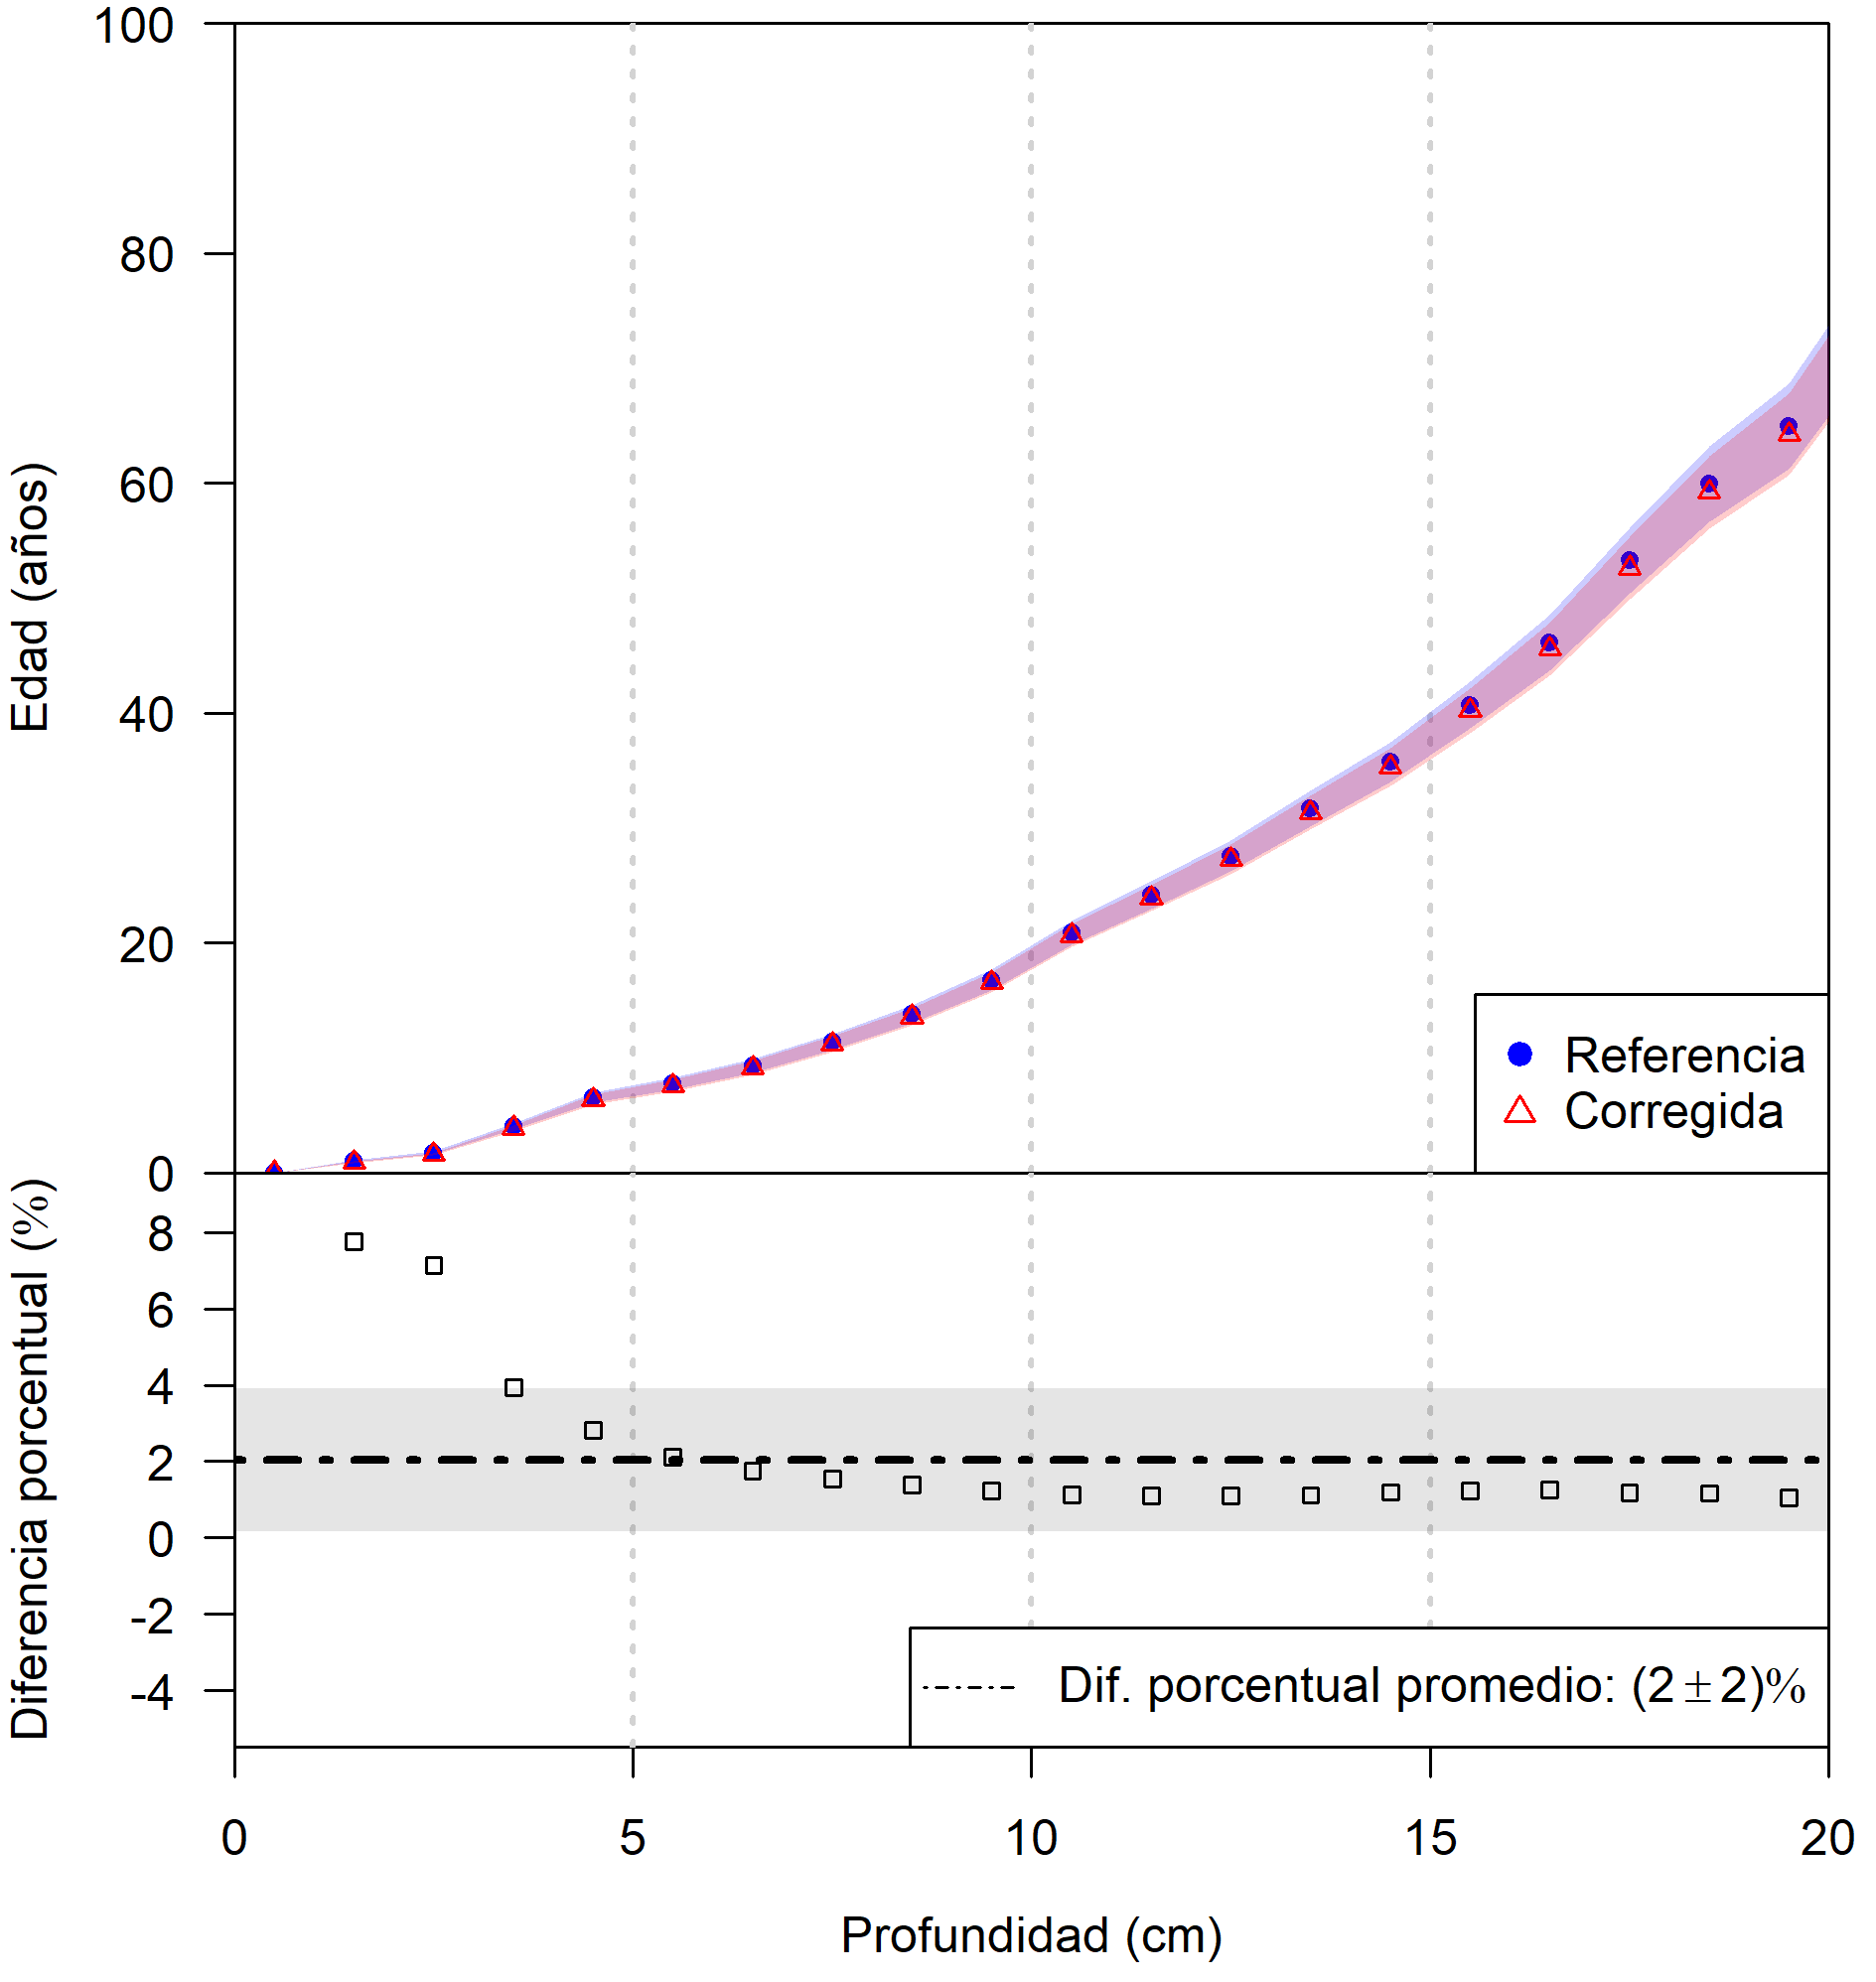
\includegraphics[width=0.9\textwidth]{Imagenes/SAMO142_1.png}
\caption{Modelo de edad del núcleo \textbf{SAMO-14-2} para la composición de referencia y la composición corregida. En la parte inferior se muestra la diferencia porcentual respecto a composición de referencia.}\label{ModeloEdad-SAMO}
\end{figure}

\begin{figure}[h]
\centering
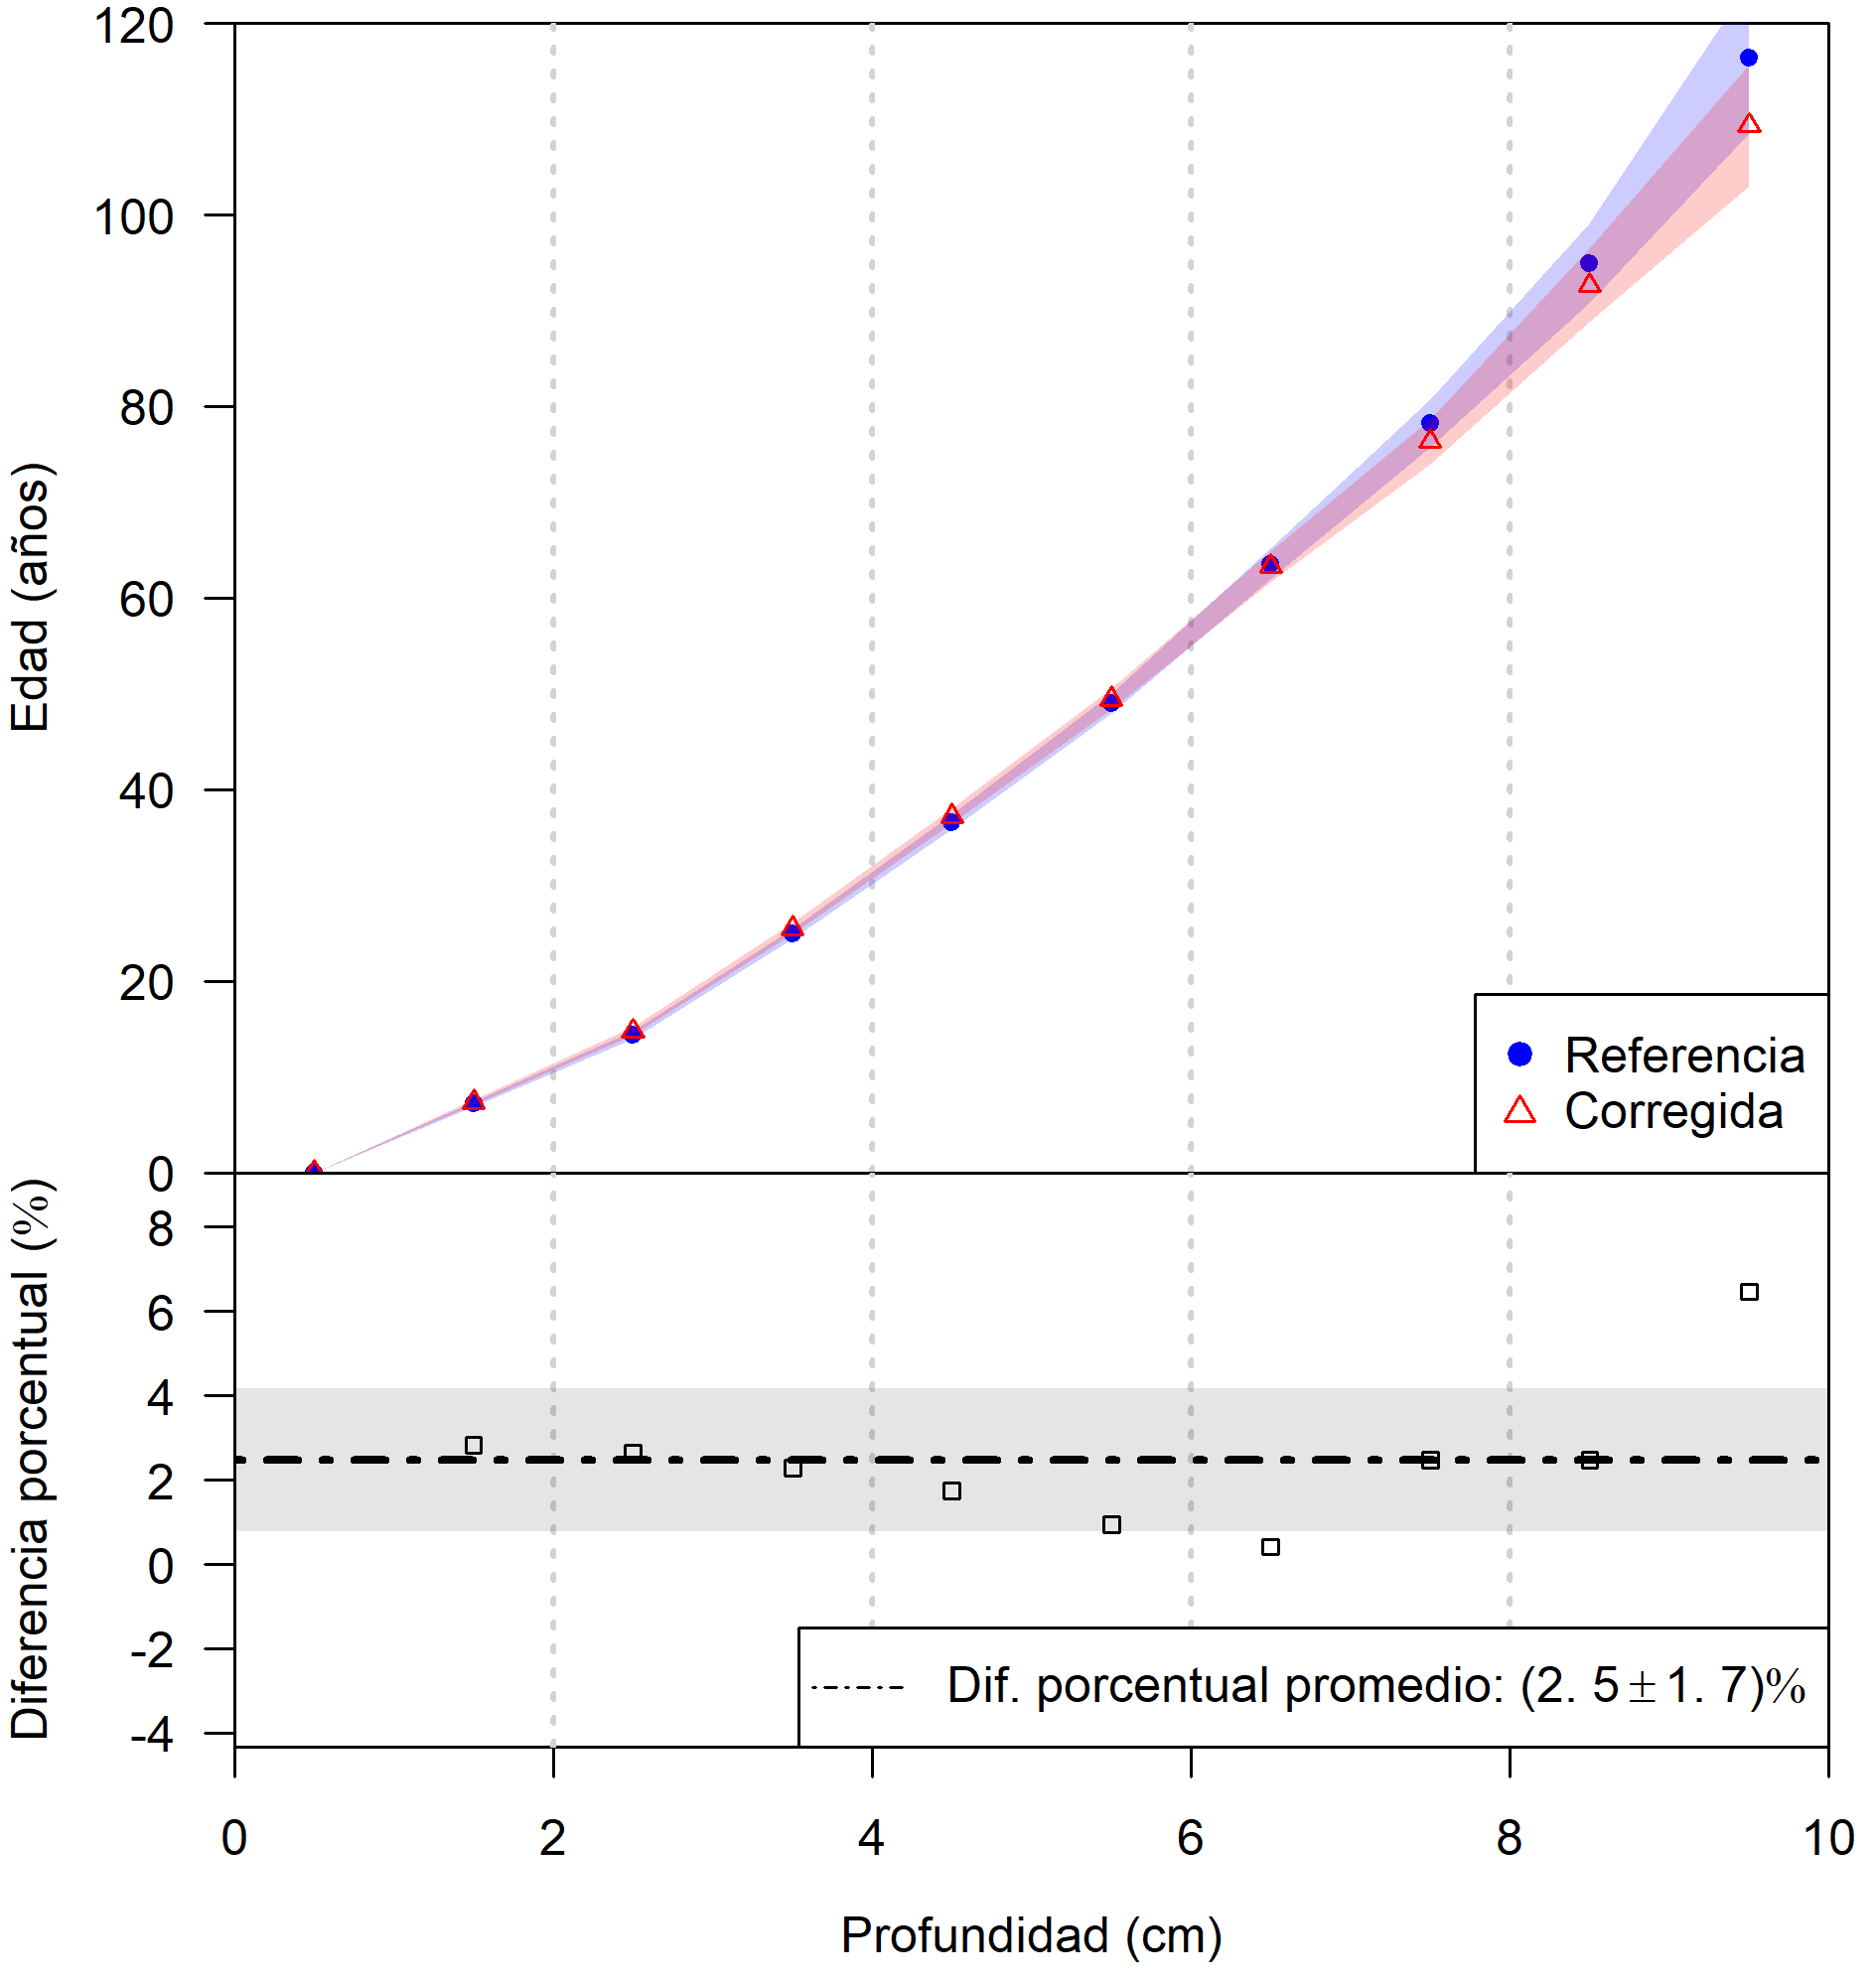
\includegraphics[width=0.9\textwidth]{Imagenes/TEHUA_1.png}
\caption{Modelo de edad del núcleo \textbf{TEHUA-XII} para la composición de referencia y la composición corregida. En la parte inferior se muestra la diferencia porcentual respecto a composición de referencia.}\label{ModeloEdad-TEHUAXII}
\end{figure}

\begin{table}[h]
\centering
\caption{Variabilidad en la diferencia porcentual promedio de las eficiencias para una energía de 46.54 keV (Tabla \ref{Tabla-Eficiencias}), variabilidad de las masas de las secciones a lo largo del núcleo y diferencia porcentual promedio entre los modelos de edad.}\label{Tabla-DiferenciasPorcentualesFechado}
\begin{tabular}{|c|c|c|c|} \hline 
\rowcolor{Blue2} & & & \\
\rowcolor{Blue2} Núcleo 			& $\dfrac{\bigtriangleup \epsilon}{\overline{\epsilon}} \times 100$ 	& $\dfrac{\bigtriangleup m}{\overline{m}} \times 100$ & Dif. promedio en modelo de edad \\
\rowcolor{Blue2} & & & \\ \hline
\rowcolor{Blue1} GOMRI-500 	& $6$ \% 								& 42 \% 			& $3\pm 2$ \% \\ 
\rowcolor{Blue1} TEHUA-XII 	&  $25$ \% 								& 16 \% 			&$2.5 \pm 1.7$ \% \\ 
\rowcolor{Blue1}LTAF 			& $33$ \% 								& 44 \% 			&$4\pm 1$ \%\\ 
\rowcolor{Blue1}PCm 				& $47$ \% 							& 17 \% 			&$0\pm 0$ \% \\
\rowcolor{Blue1} EU-VIII 			&	$8$ \% 								& 16 \% 			&$22\pm 2$ \% \\
\rowcolor{Blue1} SAMO-14-2 	&	$22$ \% 						& 32 \% 			&$2\pm 2$ \% \\
\hline
\end{tabular}
\end{table}
\chapter{Conclusiones}
\lettrine{L}{}a eficiencia de detección para \PbCero\, en los detectores utilizados en este trabajo fue del 63 al 71 \%, lo cual confirma la utilidad de la configuración de pozo para medir pequeñas muestras de material. La corrección de eficiencia por autoabsorción de cada muestra requiere el conocimiento del 100 \% de su composición elemental. El análisis elemental de los núcleos sedimentarios EU-VIII, GOMRI-500, PCm, LTAF, SAMO-14-2 y TEHUA-XII mediante la espectrometría de fluorescencia de rayos X y el análisis elemental de carbono - nitrógeno permitió constatar la gran variabilidad en la composición elemental inter- e intra-núcleos, de los que se conoce al menos el 46 \% de su composición promedio.  
\\
\\
El resto de la composición (composición desconocida) fue atribuida principalmente al H (componente mayoritario de la materia orgánica) y el oxígeno (componente mayoritario, entre otros, de los carbonatos). La diferencia promedio de utilizar del 0 al 100 \% de oxígeno para corregir la eficiencia fue de 3 \%, que es menor que la incertidumbre típica de las medidas de espectrometría de rayos gamma. Se concluyó que se podía asumir una composición desconocida con el 50 \% de contribución de oxígeno y el 50 \% de hidrógeno. 
\\
\\
La diferencia entre la eficiencia de referencia y corregida de todas las muestras varió entre 1.7 y 16 \%. Las menores diferencias fueron observadas en muestras con alta concentración de C, y por lo tanto de materia orgánica, con bajo coeficiente de atenuación de radiación gamma. Se concluyó que en los casos de alto contenido de materia orgánica, la corrección por autoabsorción no es relevante. Este fue el caso del núcleo sedimentario procedente de un manglar PCm, que presentó el mayor porcentaje de composición conocida promedio (75 \%), una diferencia promedio de 1.7 \% entre las eficiencias de referencia y corregida, y una diferencia próxima a cero entre los modelo de fechado con una composición de referencia y corregida. En este caso, no sería necesario realizar la corrección de la eficiencia por composición de la muestra. Sin embargo, siempre es importante corregir por la densidad de la muestra que puede causar desviaciones entre 0.11 hasta 0.43 g cm$^{-3}$. Aproximadamente, las desviaciones de las actividades de \PbCero\, en los núcleos sedimentarios fueron de 10 \% para EU-VIII, LTAF, SAMO-14-2 y TEHUA-XII, y de 16 \% para GOMRI-500 para composiciones de referencia y corregidas. 
\\
\\
Las desviaciones máximas observadas de las actividades corregidas (16 \%) no son inesperadas, pero sí importantes, y muestran que omitir la corrección por densidad y autoabsorción puede provocar valores de actividad de \PbCero\, demasiado bajos. Esta observación es relevante para todas las medidas de \PbCero\, (y otros radionúclidos) donde el valor absoluto de la actividad es crítico, como pueden ser los planes de vigilancia ambiental de la industria del ciclo del combustible nuclear (incluyendo la minería) y la presencia de actividades elevadas de elementos radiactivos naturales, bien sea por causas antropogénicas o no (conocidos como NORM). Esta conclusión subraya la necesidad de calibrar los sistemas de espectrometría de rayos gamma siguiendo los máximos criterios de calidad posible, y en particular la necesidad de aplicar de forma sistemática correcciones de densidad y autoabsorción, especialmente para los emisores gamma de baja energía. 
\\
\\
La cuantificación precisa de la actividad del \PbCero\, es también importante en el fechado de núcleos sedimentarios con \PbCero. Si bien se puede dar el caso de que la corrección de eficiencia sea relativamente constante y afecte poco al modelo de edad (por ejemplo, 0.1 \% para el núcleo sedimentario PCm), sí que es importante conocer con la mayor exactitud posible la profundidad a partir de la cual se puede asumir que se ha llegado al equilibrio secular. Las correcciones realizadas en este trabajo permitieron concluir que todos los núcleos sedimentarios habían llegado al equilibrio secular, condición imprescindible para realizar el fechado con el modelo CF (flujo de \PbCeroEx\, constante). 
\\
\\
Con la información disponible, incluyendo las actividades de \PbCero\, corregidas y de referencia, se realizó el fechado de los núcleos sedimentarios utilizando el modelo CF. Las fechas corregidas variaron entre 0.1 \% y 22 \%, demostrando la necesidad del uso de la corrección de la eficiencia para el fechado del \PbCero. La corrección media de los modelos de edad fue de 3 \% para GOMRI-500, 2.5 \% para TEHUA-XII, 4 \% para LTAF, 0.1 \% para PCm, 22 \% para EU-VIII y 2 \% para SAMO-14-2. Estas desviaciones medias no se correlacionaron de forma simple con la corrección de la eficiencia (y por lo tanto de la actividad) ni con su variabilidad, pues el modelo de edad incluye de forma compleja las sumas de los productos de las masas y las concentraciones. Por lo tanto, no se puede anticipar de forma simple en qué casos estas correcciones son relevantes y, por lo tanto, es necesario realizar la corrección de la densidad y eficiencia en todos los casos para obtener fechados más confiables.
\chapter{Perspectivas}
\lettrine{E}{}n primer lugar, la necesidad de realizar la corrección por densidad y composición en todas las muestras implica la integración de toda la información necesaria de forma operativa. Ello no es fácil debido a la diversidad de las técnicas utilizadas, la heterogeneidad de los resultados emitidos por los equipos y la necesidad de la intervención humana en cada uno de los pasos. 
\\
\\
Si bien se trata de un esfuerzo importante y diverso en la mayoría de los laboratorios, se propone la siguiente metodología:
\\ \\
\textbf{1.}  Crear un sistema de codificación única y completa de las muestras, con un sistema automático de detección de errores.
\\ 
\textbf{2.} Para cada uno de los equipos de análisis elemental, definición del producto final (concentraciones) en unidades absolutas, y acumulación de la información final en un servidor único. 
\\ 
\textbf{3.} En el caso de la espectrometría de rayos gamma, generar calibraciones de referencia únicas para cada detector y geometría utilizadas. No es necesario definir la densidad final de cada muestra.
\\ 
\textbf{4.} Al final (o durante) del proceso analítico, capturar de forma automática toda la información disponible de las muestras.
\\ 
\textbf{5.} Con esta información, utilizar un código para realizar la corrección de densidad y autoabsorción mediante ANGLE (o un código similar) y proporcionar las actividades corregidas de los radionúclidos de interés.
\\ \\
Una posibilidad a explorar es generar una extensa base de datos en la cual, dada la concentración de un número limitado de elementos y densidades, se pueda interpolar la corrección de eficiencia para cada muestra. Además, este ejercicio debería ser repetido para cada combinación geometría – detector de interés. Antes de abordar un proyecto de estas dimensiones, sería necesario realizar una estimación del esfuerzo de cómputo necesario y valorar el costo-beneficio del mismo. Otra posible alternativa es investigar sobre la posibilidad de utilizar modelos simplificados para realizar la estimación de la eficiencia corregida para cada muestra.
\\
\\
Una de las limitaciones de este trabajo es la necesidad de realizar aproximaciones de las concentraciones de H y O. Al menos en el caso del oxígeno, sería deseable explorar técnicas analíticas que permitan determinar este elemento de forma sistemática. Por ejemplo, el sistema \textit{Vario-Cube} de Elementar tiene esta capacidad, y se propone explorar el costo beneficio del uso de esta técnica, pues por un lado la corrección final sería menor al 3 \% y el costo del equipo y del recurso humano puede ser alto para los laboratorios que no lo tengan implementado. 
\appendix
\chapter{Códigos}\label{aped.A}
\lettrine{L}{}os códigos utilizados para integrar la información de los equipos XRF y C-N, definir el 100 \% de la composición y ejecutar ANGLE se encuentran en repositorio público 
\\ \\
\url{https://github.com/ernestocharry/CodigosMaestriaUNAM2019}
\chapter{Optimización de ANGLE}\label{SecOptANGLE}
\begin{figure}
\centering
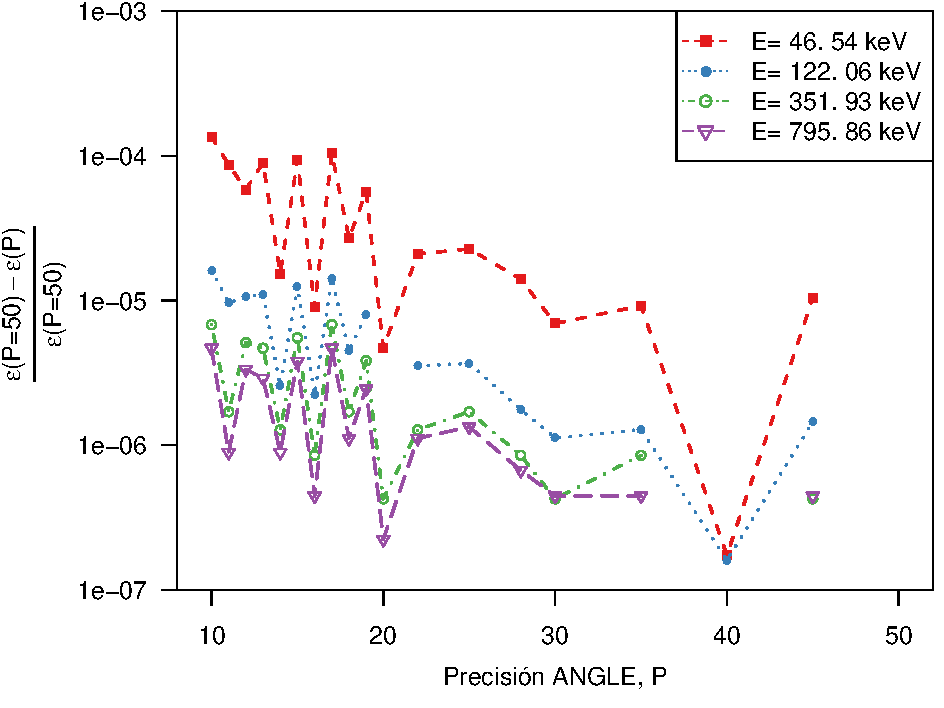
\includegraphics[width = \textwidth]{Imagenes/Eficiencia-precision-DiffPorcentual.pdf}
\caption{Gráfica de estabilidad de la eficiencia (ANGLE) para la sección 41 cm del núcleo GOMRI-500 y el sistema G2 en función de la precisión $P$ utilizada en relación a la precisión máxima, $P=50$.}\label{Fig-OptimizacionANGLE}
\end{figure}
\lettrine{E}{}l análisis de la precisión (parámetro $P$ de ANGLE) necesario para obtener los mejores resultados posibles con el mínimo esfuerzo de cómputo, se realizó utilizando la información de la sección 41 cm del núcleo GOMRI-500 con una composición desconocida del 50 \% de oxígeno. Para ello, se consideró la precisión máxima como la arrojada por el valor de $P$ máximo (50), y se calculó la diferencia respecto a este valor para diversos valores de $P$ (Figura \ref{Fig-OptimizacionANGLE}). Las diferencias observadas en todos los casos son muy pequeñas, lo que no justifica utilizar valores altos de $P$ alto. En base en el esfuerzo de cómputo requerido, se consideró adecuado utilizar un valor estándar de $P = 20$ para todos los análisis, excepto para los que requieren una simulación de Monte Carlo, para los que se utilizó el valor mínimo ($P=10$).
\chapter{Incertidumbre de la eficiencia corregida}\label{SecResulIncertidumbreEffMonteCarlo}
\begin{figure}
\centering
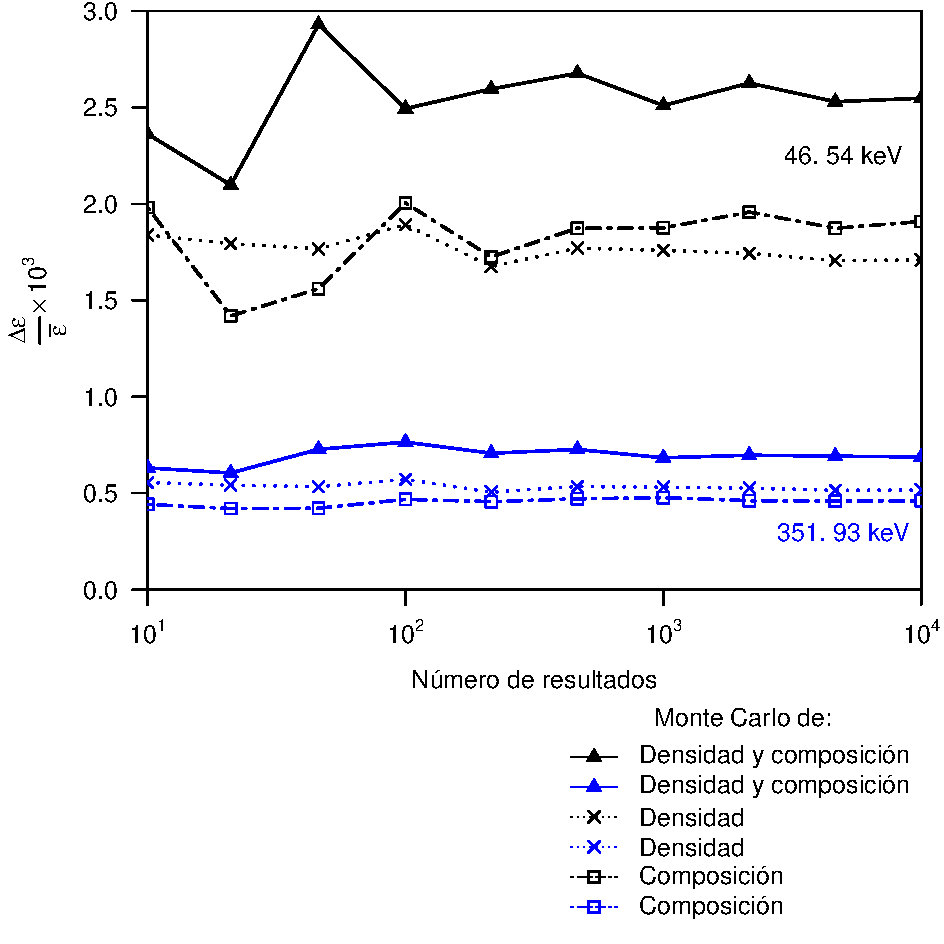
\includegraphics[width=\textwidth]{Imagenes/GOMRI-500_Eff_Point_Sec-21-75_cm.pdf}
\caption{Relación entre incertidumbre (sigma, $\Delta \epsilon$) y eficiencia promedio ($\bar{\epsilon}$) en función del número de simulaciones Monte Carlo variando el valor de la composición y / o densidad.}\label{Fig-MonteCarlo-Eficiencia}
\end{figure}
\lettrine{P}{}ara estimar la incertidumbre causada por la corrección de la eficiencia y densidad, se realizaron hasta 10$^{4}$ simulaciones con variabilidad de composición, densidad y ambas (Figura \ref{Fig-MonteCarlo-Eficiencia}). Se observó que las correcciones se estabilizan a partir de unas $10^3$ simulaciones. Las incertidumbres causadas por el proceso de corrección son muy pequeñas (Tabla \ref{Tabla-MonteCarlos-Effi}.), y fueron ignoradas en este trabajo. 
\\
\\
En este trabajo estudiamos la dependencia de la eficiencia corregida para las dos energías de interés (46.54 keV y 351.93 keV) entre 0.4 g cm$^{-3}$ y 1.5 g cm$^{-3}$, Figura \ref{Fig-EffDensidad2}. Si bien la eficiencia para el \PbCuatro\, es aproximadamente constante, para el \PbCero\, la eficiencia disminuye desde 0.66 hasta 0.53 en el intervalo de densidades analizadas.
\begin{table}
\centering
\caption{Variación de la eficiencia respecto a variaciones de la composición y/o densidad para $10^4$ repeticiones.}\label{Tabla-MonteCarlos-Effi}
\begin{tabular}{cccc}
\hline									
\rowcolor{Blue2}	Energía (keV)	&	Monte Carlo de:	&	$\bar{\epsilon} $	&	$\dfrac{\Delta \epsilon}{\bar{\epsilon}}\times 10^3 $	\\ 	\hline
\rowcolor{Blue1}	46.54	&	Composición	&	0.568255	&	1.9	\\ 	
\rowcolor{Blue1}		&	Densidad	&	0.568263	&	1.7	\\ 	
\rowcolor{Blue1}		&	Composición y densidad	&	0.568259	&	2.5	\\ 	\hline
\rowcolor{Blue1}	351.93	&	Composición	&	0.232834	&	0.5	\\ 	
\rowcolor{Blue1}		&	Densidad	&	0.232835	&	0.5	\\ 	
\rowcolor{Blue1}		&	Composición y densidad	&	0.232836	&	0.7	\\ 	\hline
\end{tabular}
\end{table}
\begin{figure}
\centering
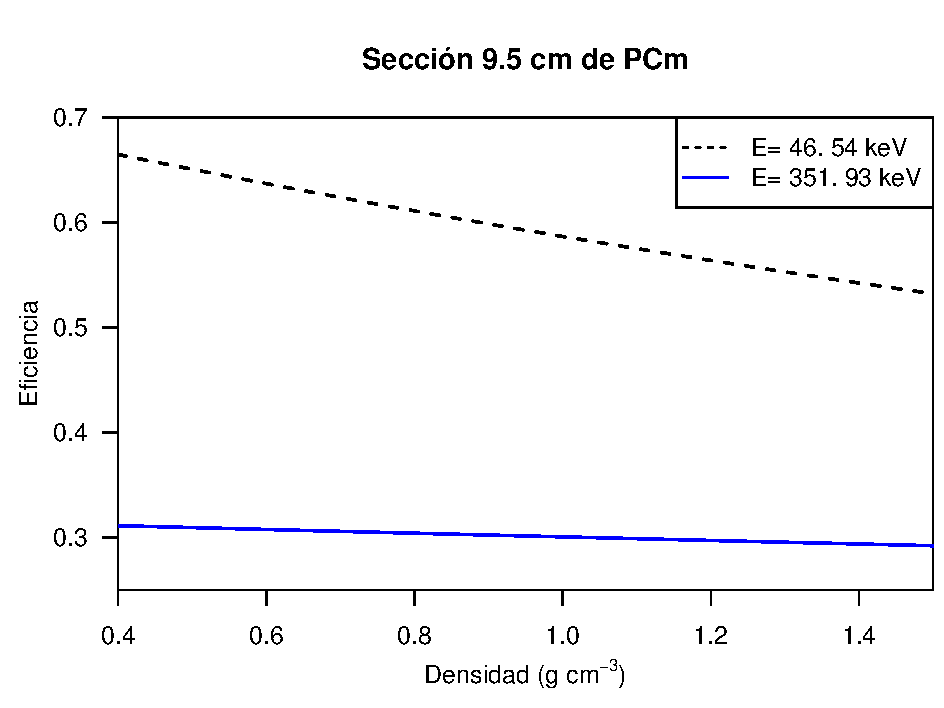
\includegraphics[width=0.9\textwidth]{Imagenes/Eficiencia-densidad.pdf}
\caption{Dependencia del valor de la eficiencia en función de la densidad para los valores de energías relacionados con \PbCero\, y \PbCuatro\, en la sección 9.5 cm del núcleo sedimentario PCm.}\label{Fig-EffDensidad2}
\end{figure}

\chapter{Secciones en equilibrio secular}\label{ApexZonaEquilibrio}
\lettrine{D}{}e acuerdo a las Figuras \ref{Fig-EUVIII-Comp}, \ref{Fig-GOMRI500-Comp}, \ref{Fig-PCm-Comp}, \ref{Fig-LTAF-Comp}, \ref{Fig-SAMO142-Comp} y \ref{Fig-TEHUAXII-Comp} se espera que en las últimas secciones de los núcleos sedimentarios exista un equilibrio secular entre \PbCero\, y \PbCuatro. En la Figura \ref{Fig-SeccEquilibrioSec} se muestra las actividades de estos radionúclidos de interés y se considera que existe un equilibrio secular en una sección cuando ambas actividades se sobreponen al considerar las incertidumbres. Estas secciones aparecen en verde en la Figura \ref{Fig-SeccEquilibrioSec}. La falta de equilibrio secular para las secciones restantes puede atribuirse a razones geoquímicas (por ejemplo, movilidad de \Ra\, en condiciones altamente reductoras), pero no debido a la corrección por composición elemental en el análisis de espectrometría de rayos gamma.
\begin{figure}
\centering
\includegraphics[width=0.9\textwidth]{Imagenes/Analisis_50Oxigeno.png}
\caption{secciones pertenecientes a la zona de equilibrio de los núcleos sedimentarios. Con $^{*}$: secciones en equilibrio secular debido a la superposición de las actividades de \PbCero\, y \PbCuatro.}\label{Fig-SeccEquilibrioSec}
\end{figure}
\chapter{Materiales de Referencia Certificados}\label{ApexMRC}
\lettrine{E}{}l estudio de la corrección de las actividades medidas de \PbCero\, y \PbCuatro\, debido a la composición elemental incluyó los cinco materiales de referencia IAEA-300, IAEA-313, IAEA-384, IAEA-385 e IAEA-448 (Tabla \ref{Table-OtrosMaterialesRefIAEA}). Se utilizó la eficiencia de referencia y la corregida por composición elemental, y los resultados se evaluaron mediante la prueba estadística $Z$-score con la actividad promedio de los materiales de referencia y su desviación estándar.
\section{Actividades específicas reportadas}
Las Figuras \ref{Fig-OutMRC-1} y \ref{Fig-OutMRC-2} muestra los gráficos de cajas de las actividades específicas (Bq kg$^{-1}$) reportadas para \PbCero\, y \PbCuatro\, correspondientes a cada material de referencia certificado. Los gráficos de cajas de las actividades se realizaron utilizando todos los valores reportados para cada material de referencia excluyendo los valores atípicos. 
\\
\\
En la Figura \ref{Fig-OutMRC-2} se observa que para IAEA-448-\PbCuatro\, los datos reportados no presentan valores atípicos y ambos gráficos de cajas son iguales (izquierda y derecha). En la Figura \ref{Fig-OutMRC-1} para IAEA-300-\PbCero\, e IAEA-313-\PbCuatro\, y en la Figura \ref{Fig-OutMRC-2} para IAEA-385-\PbCero\, se observa que, después de descartar los valores atípicos, la distribución de la actividad específica no vuelve a presentar valores atípicos. En los demás casos (IAEA-300-\PbCuatro, IAEA-384-\PbCero, IAEA-384-\PbCuatro\, e IAEA-385-\PbCuatro), después de eliminar los primeros valores atípicos, la distribución encontrada de la actividad específica sigue presentando valores atípicos que no son eliminados para no producir distribuciones lejanas a la original de cada proceso de certificación.
\begin{figure}
\centering 
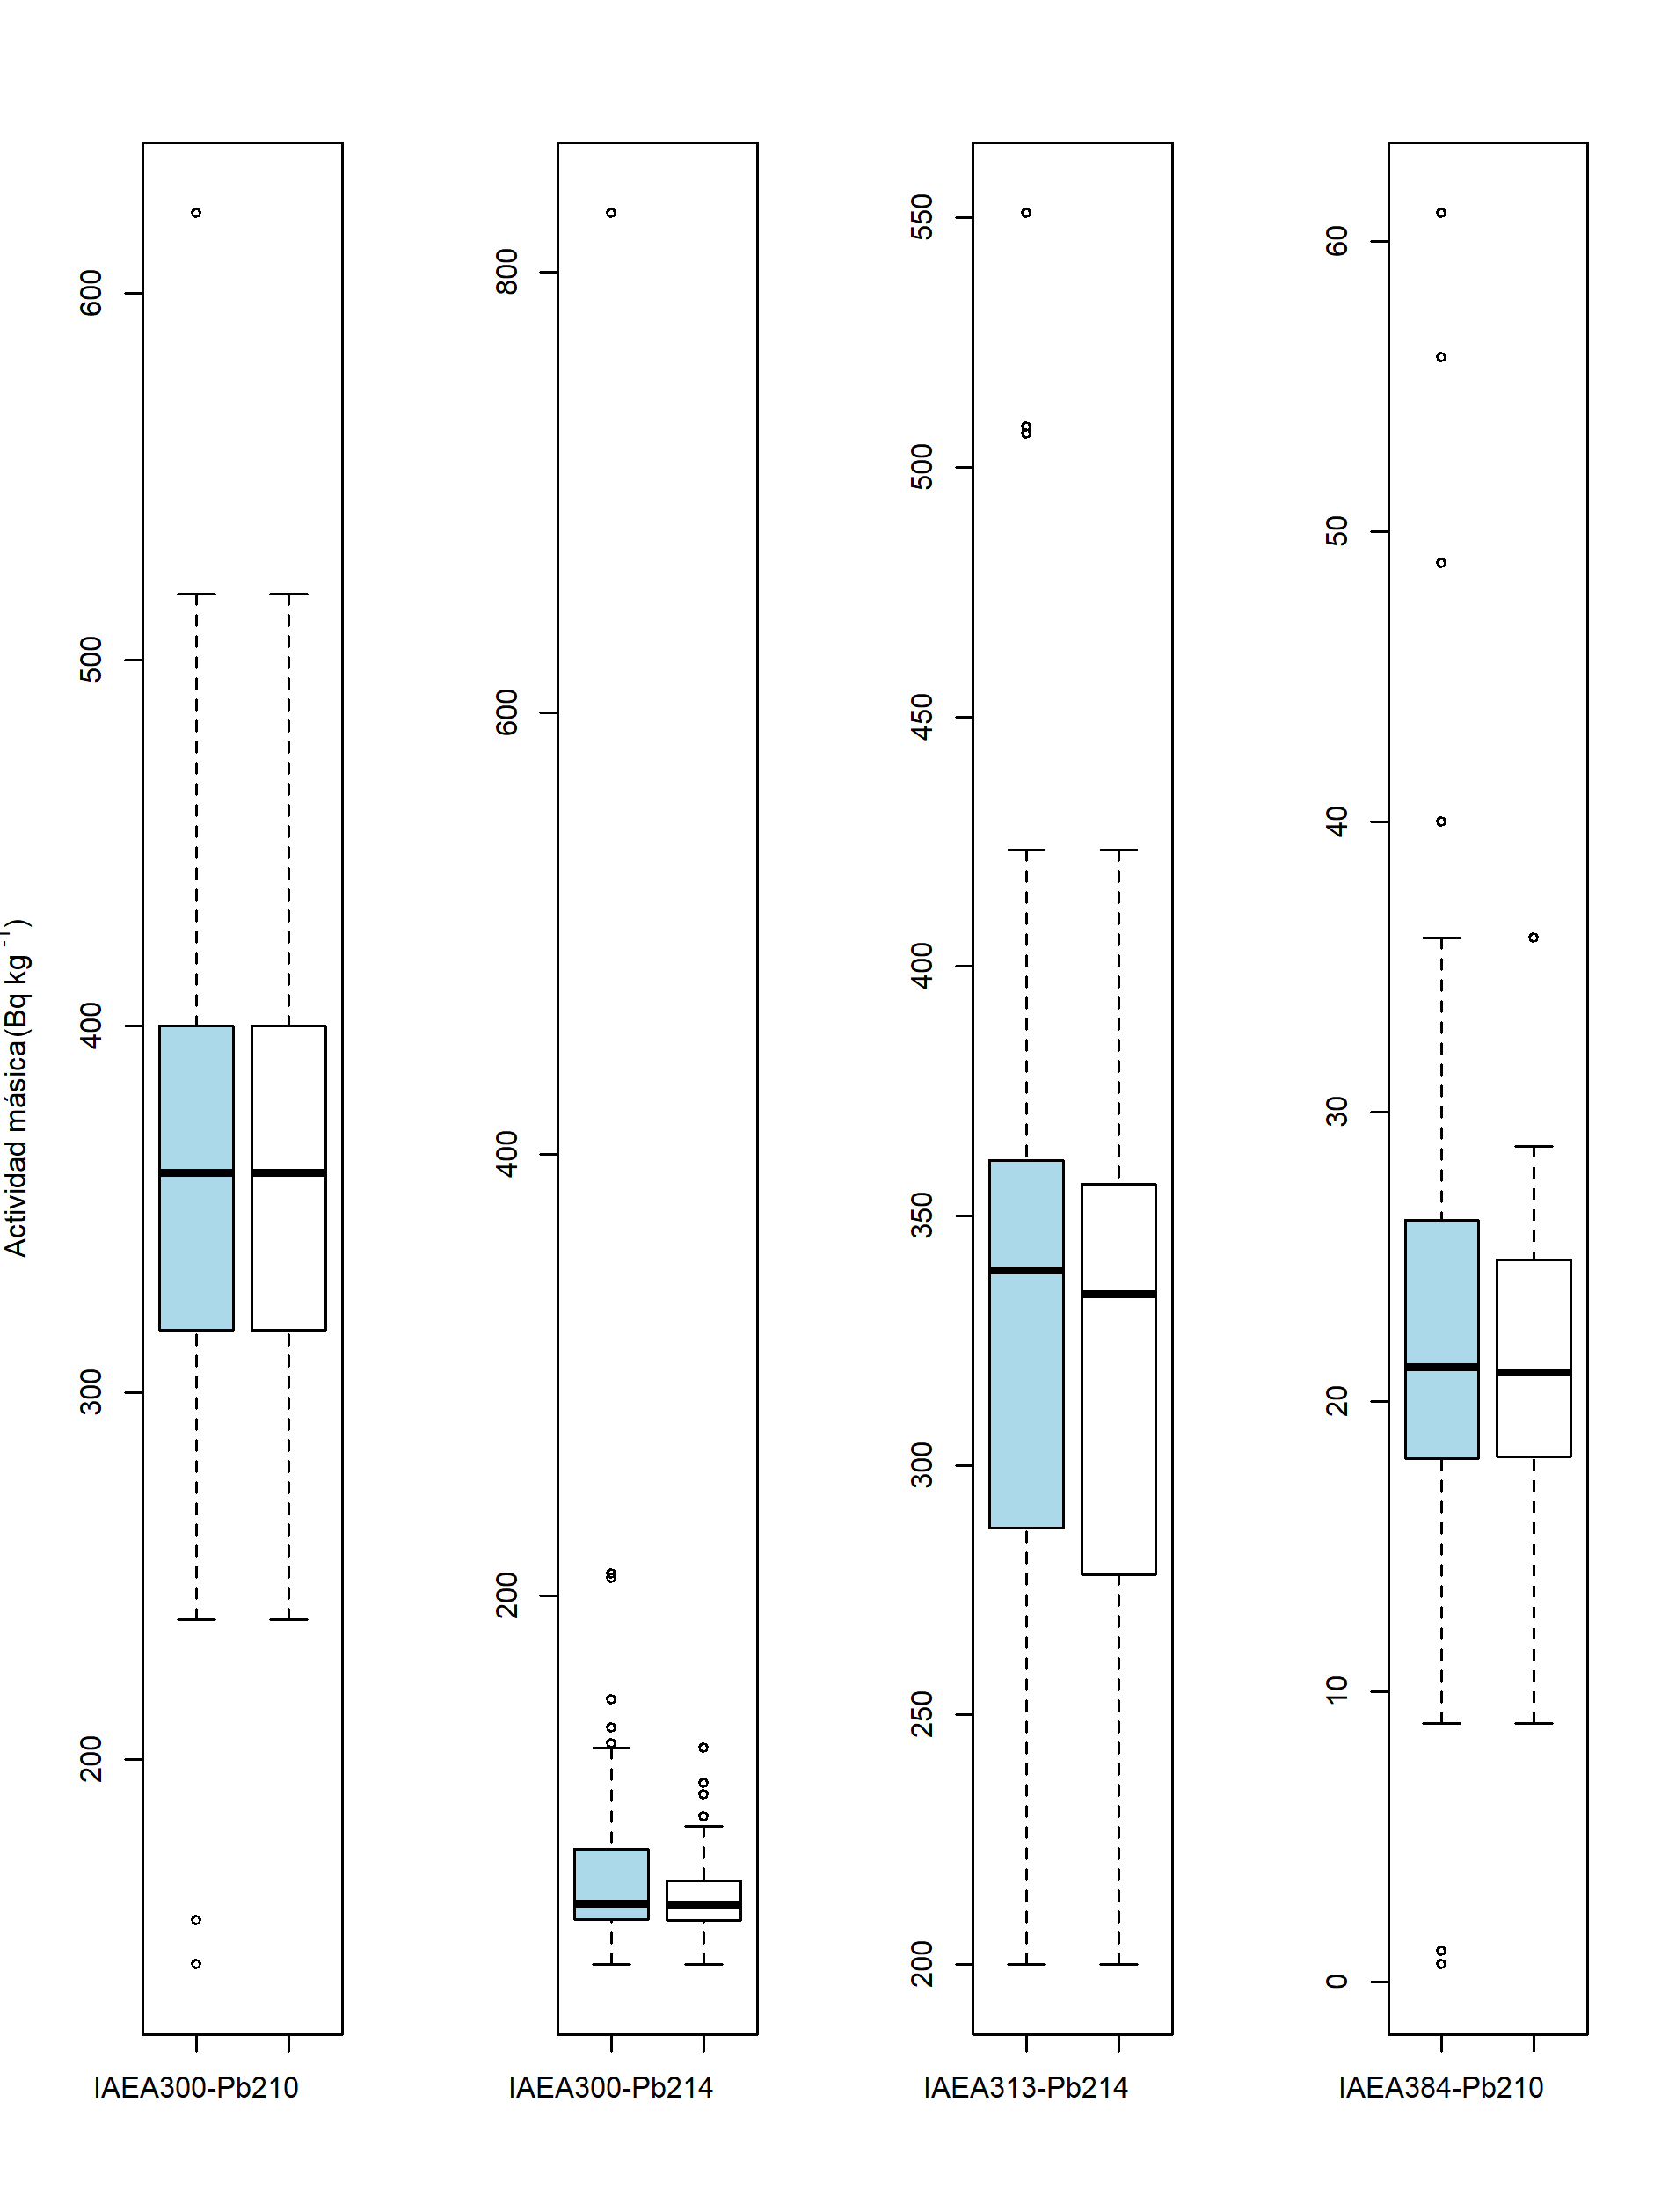
\includegraphics[width=0.9\textwidth]{Imagenes/PlotOutliers-1-IAEA-All.png}
\caption{Diagramas de cajas y valores atípicos de las actividades específicas de \PbCero\, y \PbCuatro\, reportadas para los materiales de referencias IAEA-300, IAEA-313 e IAEA-384. Izquierda: utilizando todos los valores reportados, derecha: excluyendo los primeros valores atípicos.  }\label{Fig-OutMRC-1}
\end{figure}
\begin{figure}
\centering 
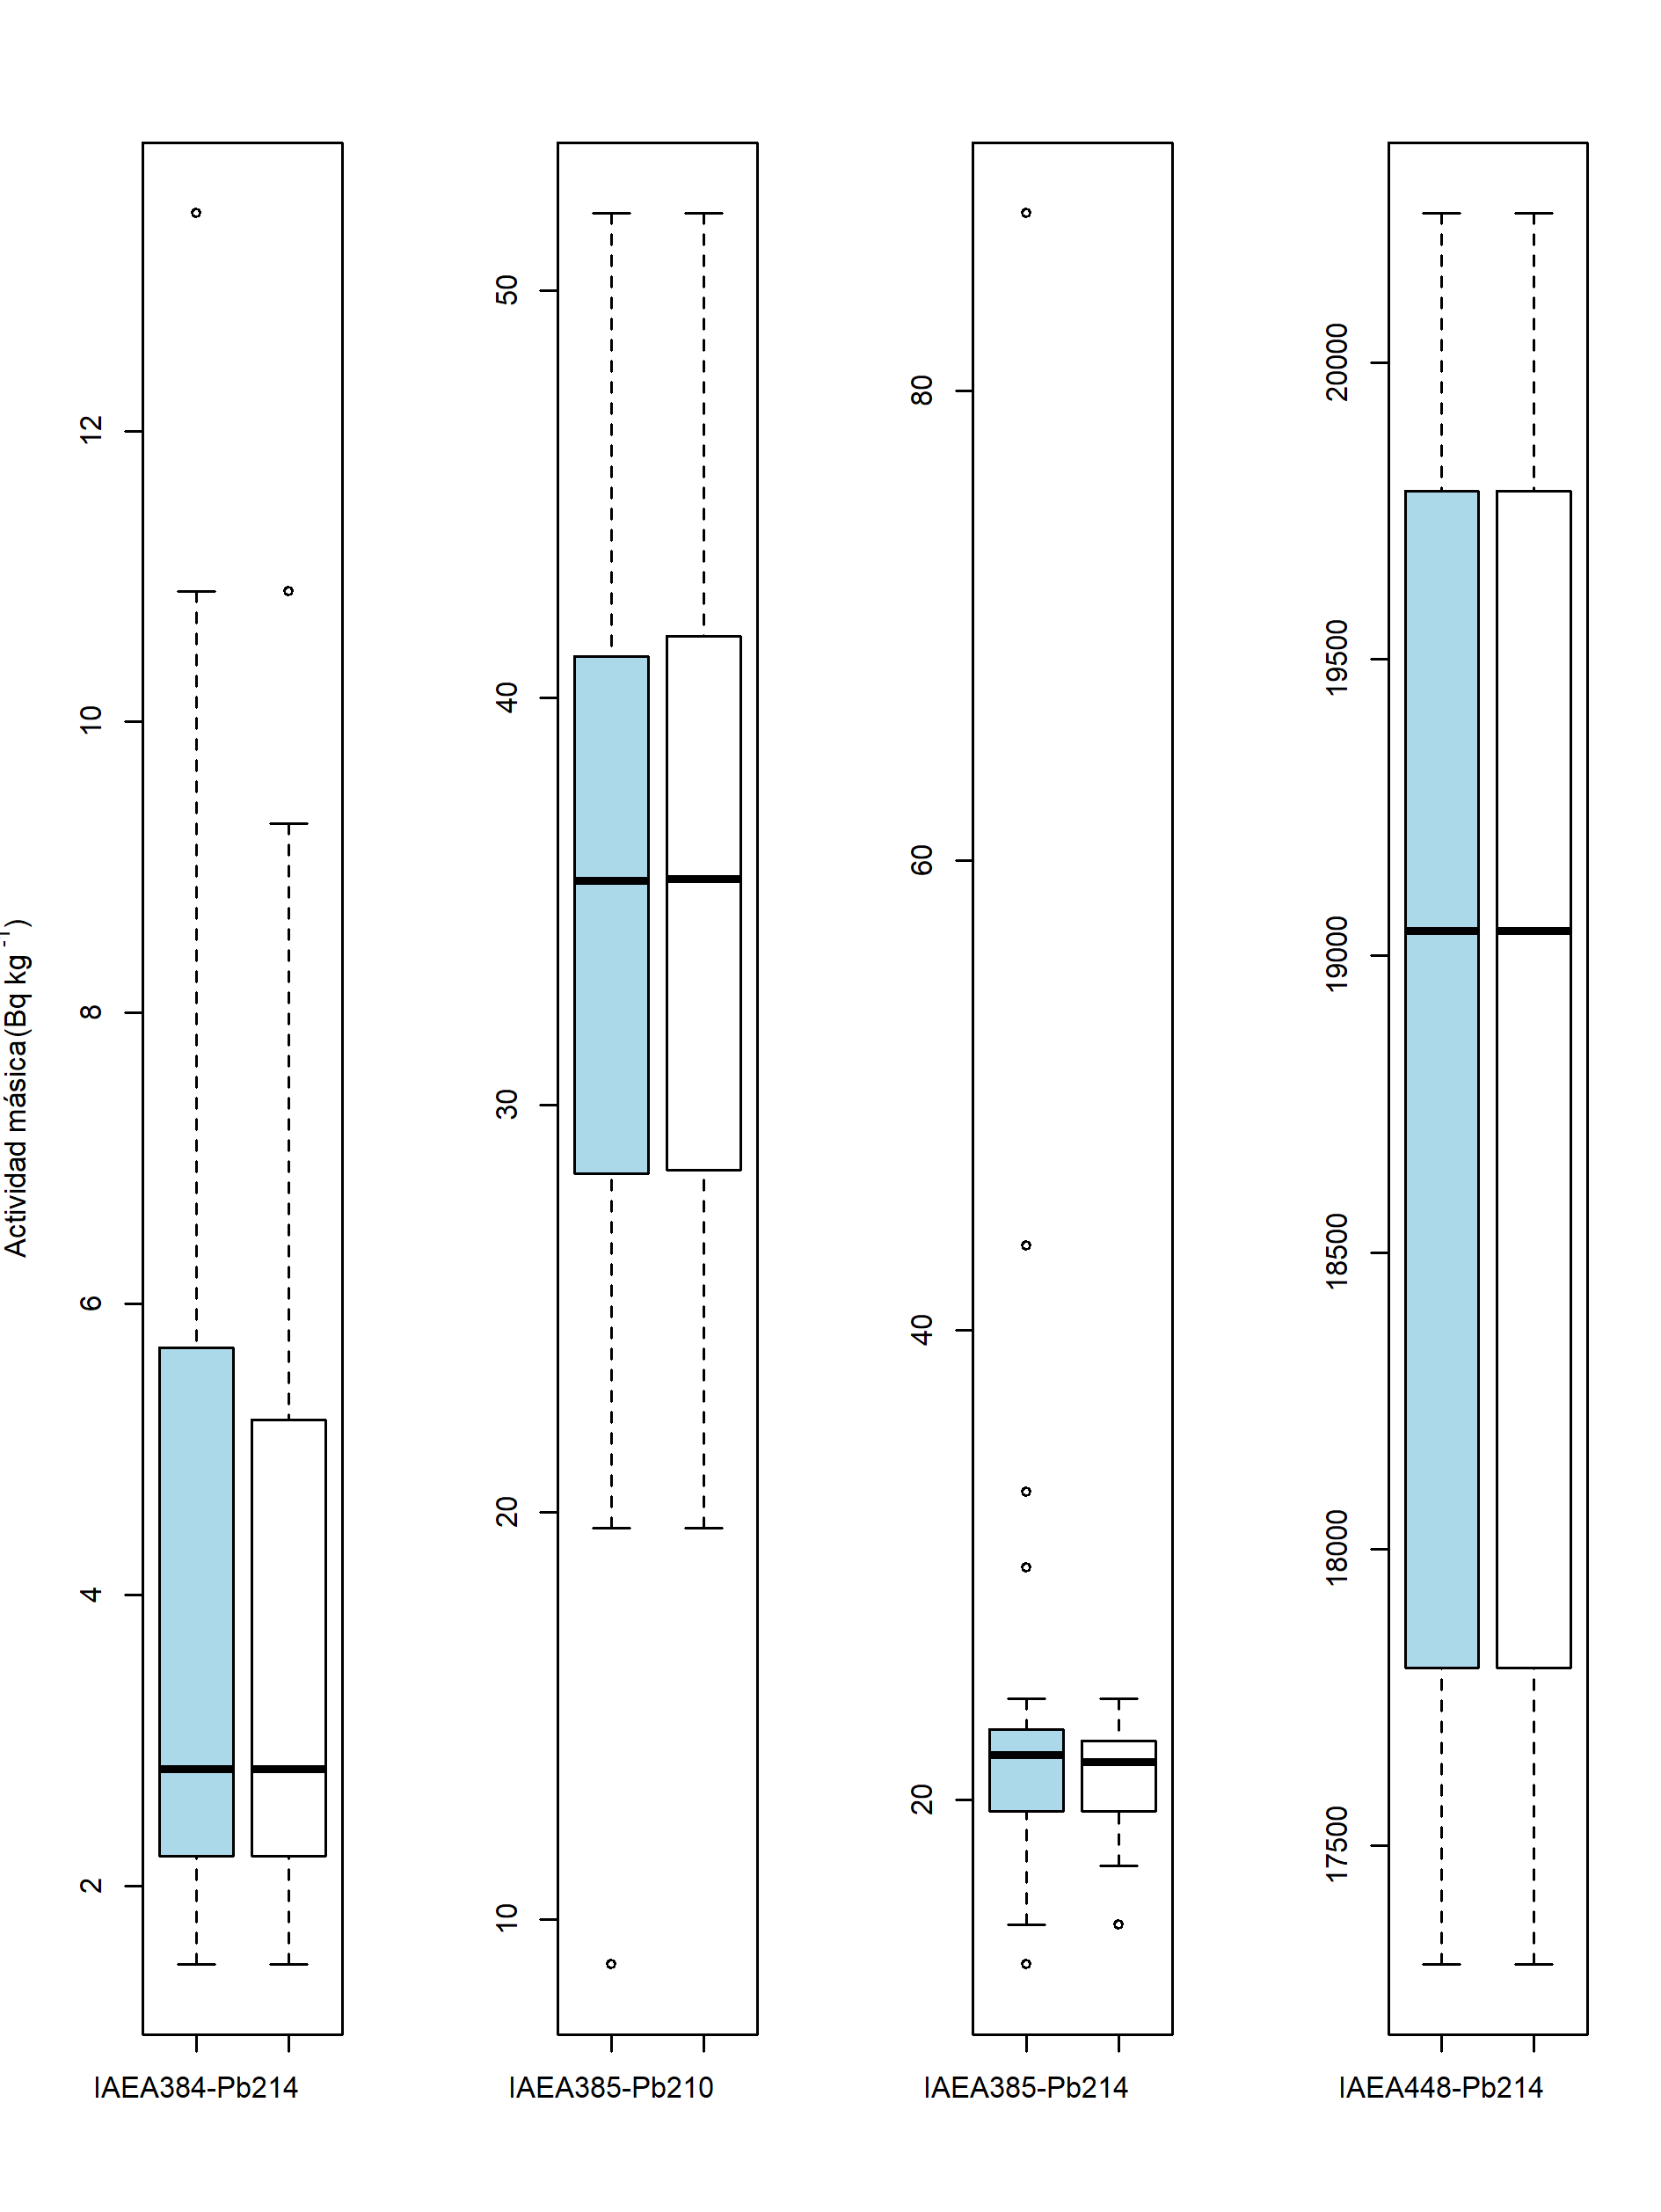
\includegraphics[width=0.9\textwidth]{Imagenes/PlotOutliers-2-IAEA-All.png}
\caption{Diagrama de cajas y valores atípicos de las actividades específicas de \PbCero\, y \PbCuatro\, reportadas para los materiales de referencias IAEA-384, IAEA-385 e IAEA-448. Izquierda: utilizando todos los valores reportados, derecha: excluyendo los primeros valores atípicos. }\label{Fig-OutMRC-2}
\end{figure}
\\
\\
Si se tiene $n$ mediciones de una variable tal que cada medición sea $x_i \pm \sigma_i$, $1\leq i\leq n$, entonces el promedio $\overline{x}$ y la desviación estándar total $\sigma$ es
\begin{eqnarray}
\overline{x} &=& \dfrac{1}{n}\sum_i^n x_i \\
\sigma^2_\text{int} &=& \dfrac{1}{n^2} \sum_i^n \sigma_i^2 \\
\sigma^2_\text{ext} &=& \dfrac{1}{n-1}\sum_i^n (x_i-\overline{x})^2 \\
\sigma &=& \sqrt{\sigma^2_\text{ext}  + \sigma^2_\text{int}}
\end{eqnarray}
donde $\sigma^2_\text{int}$ es la desviación estándar de todos los valores en relación a la media, y $\sigma^2_\text{ext}$ tiene en cuenta la incertidumbre de cada valor reportado. Los resultados se presentan en la Tabla \ref{Table-MRC}. 
\begin{table}
\centering
\caption{Actividad específica promedio $\overline{x}$ y desviación estándar $\sigma$ de Materiales de Referencia Certificados para \PbCero\, y \PbCuatro. Se incluye los valores de los percentiles 0.025 y 0.975}\label{Table-MRC}
\begin{tabular}{|c|c|c|c|c|c|}
\hline													
\rowcolor{Blue2}	MRC	&	No. de Datos	&	$\overline{x}$	&	$\sigma$	&	2.5 \% 	&	97.5 \% 	\\ 	\hline
\rowcolor{Blue1}	IAEA300-\PbCero	&	46	&	364.5	&	57.5	&	275.5	&	478.7	\\ 	
\rowcolor{Blue1}	IAEA300-\PbCuatro	&	66	&	65.1	&	19.7	&	38.8	&	111.9	\\ 	
\hline
\rowcolor{Blue1}	IAEA313-\PbCuatro	&	21	&	317.2	&	53.8	&	207.9	&	395.7	\\ 	
\hline
\rowcolor{Blue1}	IAEA384-\PbCero	&	29	&	21.2	&	5.6	&	11.1	&	31.0	\\ 	
\rowcolor{Blue1}	IAEA384-\PbCuatro	&	13	&	4.0	&	3.0	&	1.6	&	10.4	\\ 	
\hline
\rowcolor{Blue1}	IAEA385-\PbCero	&	44	&	35.1	&	7.8	&	22.4	&	46.0	\\ 	
\rowcolor{Blue1}	IAEA385-\PbCuatro	&	21	&	20.8	&	2.4	&	16.0	&	23.7	\\ 	
\hline
\rowcolor{Blue1}	IAEA448-\PbCuatro	&	6	&	18870.2	&	1202.3	&	17362.5	&	20194.3	\\ 	\hline
\end{tabular}
\end{table}
\section{Corrección y comparación de las actividades}
La Tabla \ref{Table-ZScoreResultados} muestra las actividades específicas de los MRC para la composición de referencia y la composición corregida. La composición corregida para los MRC se determinó de manera análoga al procedimiento descrito para las secciones de los núcleos sedimentarios (Sección \ref{Secc-100Composicion}) en donde se asume una composición estándar de 50 \% oxígeno. Estas actividades se encuentran corregidas para las fechas de referencia reportadas en los certificados de los materiales de referencia (Tabla \ref{Table-MRC}). 
\\
\\
La corrección en el tiempo de la actividad total de \PbCero\, ($^{210}$Pb$_\text{total}$) se realiza utilizando la ley de desintegración radiactiva y el semiperiodo $T_{\frac{1}{2}}$ adecuado para el \PbCeroBa\, y \PbCeroEx\, (Ecuación \ref{Eq-PbTotal}). Debido a la geoquímica de Pb, el semiperiodo de \PbCeroBa\, es el semiperiodo de \Ra\, (1600 años) \cite{DataDecayEvaluation} y el semiperiodo de \PbCeroEx\, corresponde al semiperiodo de \PbCero\, (22.23 años) \cite{DataDecayEvaluation}. 
\\
\\
Para la intercomparación de los resultados se utilizó $Z$-score, que se define como 
\begin{equation}\label{Eq-Zscore}
Z = \dfrac{| \overline{x} - \overline{x}_m | }{\sqrt{\sigma^2 + \sigma_m^2}}
\end{equation}
donde $\overline{x}$ y $\sigma$ es la actividad másica promedio y desviación estándar reportada (Tabla \ref{Table-MRC}), $\overline{x}_m$ y $\sigma_m$ es la actividad másica promedio y desviación estándar medida, asumiendo una composición de referencia o una composición corregida. Un resultado es aceptable si $Z \leq 2$, que equivale al criterio del 95 \%. \\
\begin{table}
\centering
\caption{Actividad y desviación estándar medida asumiendo una composición de referencia y la eficiencia de referencia y una referencia corregida por la composición. }\label{Table-ZScoreResultados}
\begin{tabular}{|c|c|c|c|cc|c|}
\hline																					
\rowcolor{Blue3}	MRC	&	Actividad certificado 			&	Actividad Ref.			&	Actividad Corr.			&	\multicolumn{2}{|c|}{$Z$}     			&	$\Delta Z$	\\	\hline
\rowcolor{Blue3}	IAEA-	&	Bq kg$^{-1}$			&	Bq kg$^{-1}$			&	Bq kg$^{-1}$			&	Ref.	&	Corr.	&		\\	\hline
\rowcolor{Blue2}	\multicolumn{7}{|l|}{\PbCero}     																			\\	\hline
\rowcolor{Blue1}	385	&	35.1 (7.8)			&	22.0 (11.3)			&	29.9 (13.4)			&	1.0	&	0.3	&	0.6	\\	
\rowcolor{Blue1}	384	&	21.2 (5.6)			&	26.7 (8.1)			&	36.1 (10.2)			&	0.6	&	1.3	&	-0.7	\\	
\rowcolor{Blue1}	300	&	364.5 (57.5)			&	183.8 (31.1)			&	227.5 (36.5)			&	2.8	&	2.0	&	0.8	\\	\hline
\rowcolor{Blue2}	\multicolumn{7}{|l|}{\PbCuatro}     																			\\	\hline
\rowcolor{Blue1}	313	&	317.2 (53.8)			&	327.1 (10.5)			&	337.4 (10.8)			&	0.2	&	0.4	&	-0.2	\\	\hline
\rowcolor{Blue1}	384	&	4.0 (3.0)			&	5.0 (0.7)			&	5.2 (0.7)			&	0.34	&	0.38	&	-0.04	\\	\hline
\rowcolor{Blue1}	300	&	65.1 (19.7)			&	49.9 (4.5)			&	50.6 (4.5)			&	0.7	&	0.7	&	0.0	\\	\hline
\rowcolor{Blue1}	385	&	20.8 (2.4)			&	25.0 (1.3)			&	25.7 (1.4)			&	1.5	&	1.8	&	-0.2	\\	\hline
\rowcolor{Blue1}	448	&	18870.2 (1202.3)			&	15732.7 (495.5)			&	16021.7 (504.6)			&	2.4	&	2.2	&	0.2	\\	\hline

\end{tabular}
\end{table}
\begin{figure}
\centering
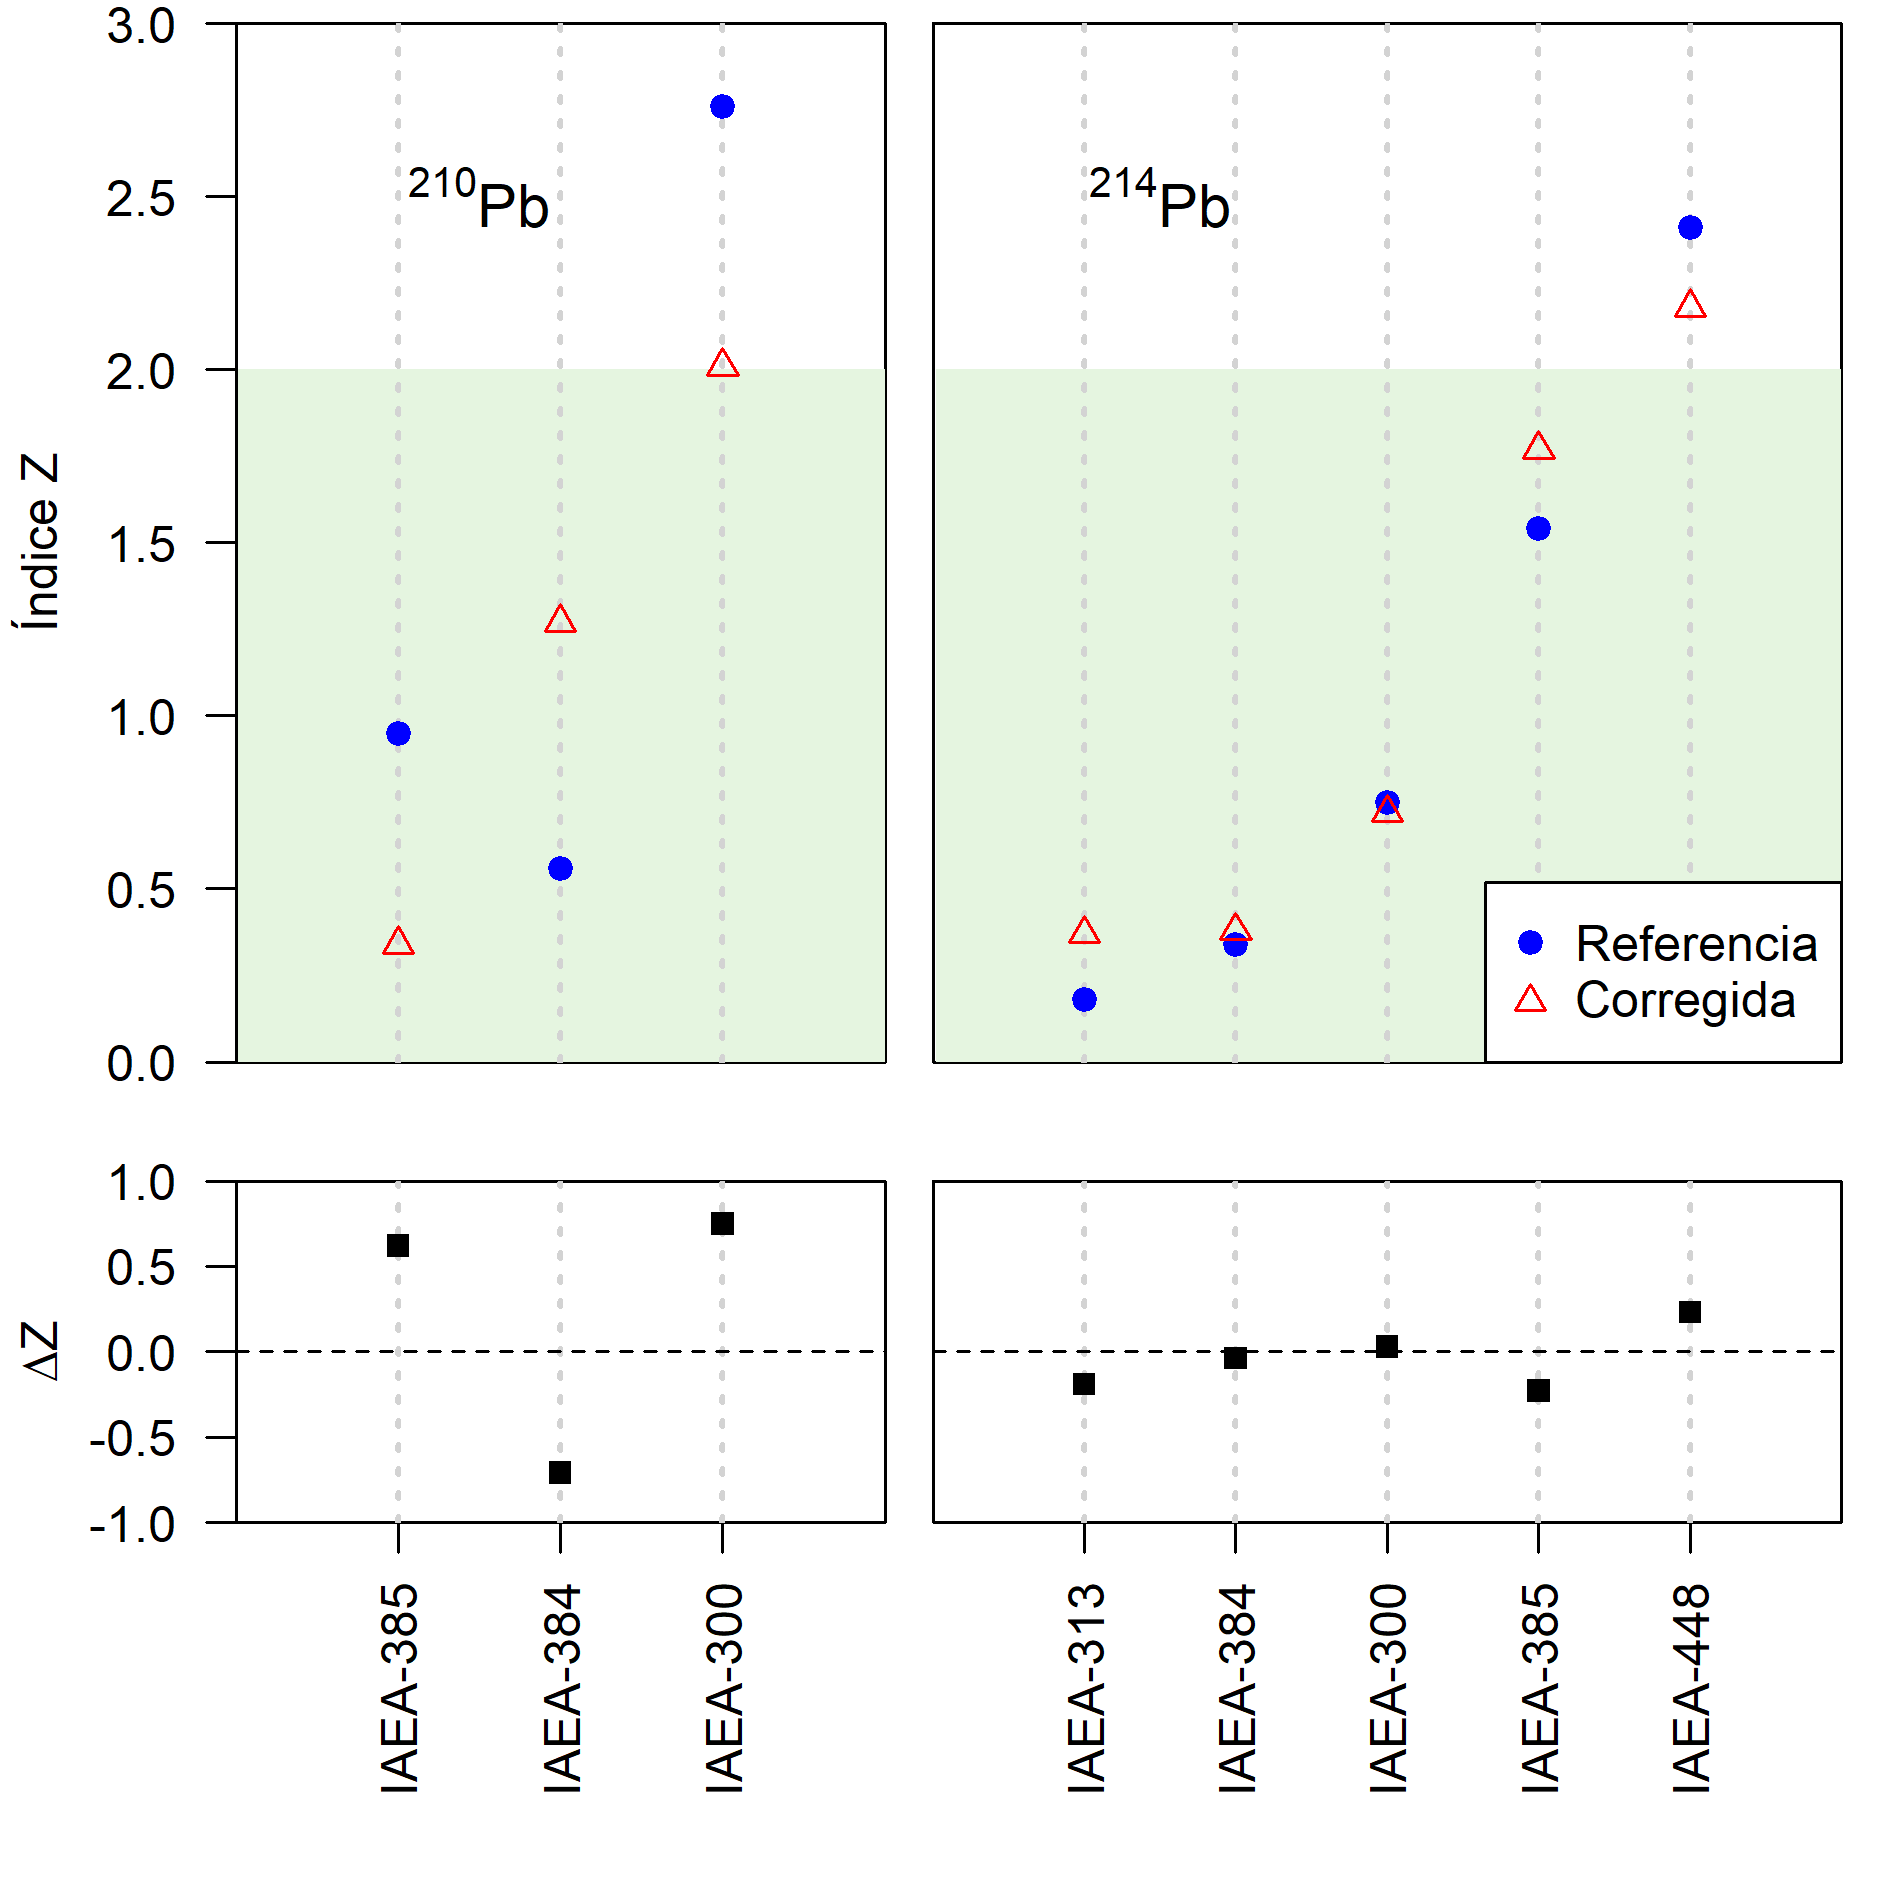
\includegraphics[width=0.9\textwidth]{Imagenes/Z-score-results.png}
\caption{Índice $Z$ y desviación $\Delta Z$ para las actividades másicas de materiales de referencia certificados utilizando una eficiencia de referencia y una eficiencia corregida por la composición.}\label{Fig-ZScore}
\end{figure}
\\De acuerdo a los resultados de la Tabla \ref{Table-ZScoreResultados} y a la Figura \ref{Fig-ZScore} se observa que dos (IAEA-385 e IAEA-384) de los tres MRC presentan resultados aceptables para \PbCero\, y cuatro (IAEA-313, IAEA-384, IAEA-300 E IAEA-385) de los cinco MRC presentan resultados aceptables para \PbCuatro\, puesto que el índice $Z$ es menor a dos en estos casos. 
\\ \\ 
También se observa que $\Delta Z$ para los resultados de las actividades utilizando una composición de referencia y una composición corregida es mayor para \PbCero\, ($|\Delta Z|$ > 0.5 en todos los casos) que para \PbCuatro\, ($|\Delta Z|$ < 0.5 en todos los casos). Lo anterior es debido a la dependencia de la eficiencia respecto a la composición - densidad para las energías relacionadas con los radionúclidos. 
\\ \\ 
La corrección de las actividades de \PbCero\, por la composición elemental disminuyó el índice $Z$ para los MRC IAEA-385 e IAEA-300 en comparación con los resultados en donde se utilizó una composición de referencia. Sin embargo, el MRC IAEA-384 produce mejores resultados cuando se asume una composición de referencia. Por otra parte, la corrección de las actividades de \PbCuatro\, por la composición elemental disminuye el índice $Z$ para los MRC IAEA-300 e IAEA-448. Para los MRC IAEA-313, IAEAE-384 e IAEA-385, los resultados producen menores índices Z cuando se asume una composición de referencia que cuando se asume una composición corregida, aunque ambas composiciones generan resultados aceptables ($Z$ < 2). 
\\ \\ 
En los resultados del índice $Z$ para los dos radionúclidos (\PbCero\, y \PbCuatro) se observa que IAEA-384 e IAEA-300 presentan el mismo comportamiento aunque diferentes $\Delta Z$. El índice $Z$ es mayor tanto para la actividad corregida de \PbCero\, y \PbCuatro\, en IAEA-384, como para la actividad de referencia en IAEA-300. En contraste, para el MRC IAEA-385, los índices $Z$ fueron menores para las actividades de \PbCero\, corregidas por la composición elemental, así como para las actividades \PbCuatro\, determinadas a partir de una composición de referencia.

\bibliographystyle{apalike-es}
\bibliographystyle{plain}
\bibliography{Bibliography}
\end{document}